% Generated by Sphinx.
\def\sphinxdocclass{report}
\documentclass[a4paper,10pt]{sphinxmanual}
\usepackage[T1]{fontenc}
\usepackage[ngerman]{babel}
\usepackage{times}
\usepackage[Sonny]{fncychap}
\usepackage{longtable}
\usepackage{sphinx}
\usepackage{multirow}

\usepackage[a4paper,margin=2cm,rmargin=2.3cm,tmargin=2cm]{geometry}
%% \geometry{verbose,tmargin=1cm,bmargin=2.5cm,lmargin=2.5cm,rmargin=2.5cm,headheight=3cm,headsep=1cm,footskip=1cm}

\definecolor{TitleColor}{rgb}{0.212, 0.376, 0.569}
%% \definecolor{InnerLinkColor}{rgb}{0.0, 0.0, 0.4}
\definecolor{InnerLinkColor}{rgb}{1.0, 0.0, 0.0}
\renewcommand{\familydefault}{\sfdefault}

\usepackage{fontspec}
\setmainfont[Mapping = tex-text, FakeStretch = 1.04, WordSpace = 1.7]{FreeSerif}
\setsansfont[Mapping = tex-text, FakeStretch = 1.04, WordSpace = {1.2, 1.7, 1.0}]{FreeSans}

\usepackage{setspace}
\setstretch{1.2}

\usepackage{xunicode}

\usepackage{csquotes}
\usepackage{enumerate}

\usepackage[style=alphabetic,backend=biber]{biblatex}
\addbibresource{links.bib}
\addbibresource{ai4.bib}
\addbibresource{komplett2.bib}

\setlength{\parskip}{\medskipamount}
\setlength{\parindent}{0pt} 

\usepackage{pdfpages}

\def\sectionautorefname{Kap.}
\def\subsectionautorefname{Kap.}
\def\chapterautorefname{Kap.}

\setcounter{tocdepth}{2}




\title{
i>PM 3D -- Ein Prozessmodellierungswerkzeug für drei Dimensionen \\
\vspace{1cm}
Repräsentation von Prozessmodellen im dreidimensionalen Raum -- Konzept und Implementierung
}
\date{12. 04. 2012}
\author{Tobias Stenzel}
\newcommand{\sphinxlogo}{}
\makeindex

\makeatletter
\def\PYG@reset{\let\PYG@it=\relax \let\PYG@bf=\relax%
    \let\PYG@ul=\relax \let\PYG@tc=\relax%
    \let\PYG@bc=\relax \let\PYG@ff=\relax}
\def\PYG@tok#1{\csname PYG@tok@#1\endcsname}
\def\PYG@toks#1+{\ifx\relax#1\empty\else%
    \PYG@tok{#1}\expandafter\PYG@toks\fi}
\def\PYG@do#1{\PYG@bc{\PYG@tc{\PYG@ul{%
    \PYG@it{\PYG@bf{\PYG@ff{#1}}}}}}}
\def\PYG#1#2{\PYG@reset\PYG@toks#1+\relax+\PYG@do{#2}}

\def\PYG@tok@gd{\def\PYG@tc##1{\textcolor[rgb]{0.63,0.00,0.00}{##1}}}
\def\PYG@tok@gu{\let\PYG@bf=\textbf\def\PYG@tc##1{\textcolor[rgb]{0.50,0.00,0.50}{##1}}}
\def\PYG@tok@gt{\def\PYG@tc##1{\textcolor[rgb]{0.00,0.25,0.82}{##1}}}
\def\PYG@tok@gs{\let\PYG@bf=\textbf}
\def\PYG@tok@gr{\def\PYG@tc##1{\textcolor[rgb]{1.00,0.00,0.00}{##1}}}
\def\PYG@tok@cm{\let\PYG@it=\textit\def\PYG@tc##1{\textcolor[rgb]{0.25,0.50,0.56}{##1}}}
\def\PYG@tok@vg{\def\PYG@tc##1{\textcolor[rgb]{0.73,0.38,0.84}{##1}}}
\def\PYG@tok@m{\def\PYG@tc##1{\textcolor[rgb]{0.13,0.50,0.31}{##1}}}
\def\PYG@tok@mh{\def\PYG@tc##1{\textcolor[rgb]{0.13,0.50,0.31}{##1}}}
\def\PYG@tok@cs{\def\PYG@tc##1{\textcolor[rgb]{0.25,0.50,0.56}{##1}}\def\PYG@bc##1{\colorbox[rgb]{1.00,0.94,0.94}{##1}}}
\def\PYG@tok@ge{\let\PYG@it=\textit}
\def\PYG@tok@vc{\def\PYG@tc##1{\textcolor[rgb]{0.73,0.38,0.84}{##1}}}
\def\PYG@tok@il{\def\PYG@tc##1{\textcolor[rgb]{0.13,0.50,0.31}{##1}}}
\def\PYG@tok@go{\def\PYG@tc##1{\textcolor[rgb]{0.19,0.19,0.19}{##1}}}
\def\PYG@tok@cp{\def\PYG@tc##1{\textcolor[rgb]{0.00,0.44,0.13}{##1}}}
\def\PYG@tok@gi{\def\PYG@tc##1{\textcolor[rgb]{0.00,0.63,0.00}{##1}}}
\def\PYG@tok@gh{\let\PYG@bf=\textbf\def\PYG@tc##1{\textcolor[rgb]{0.00,0.00,0.50}{##1}}}
\def\PYG@tok@ni{\let\PYG@bf=\textbf\def\PYG@tc##1{\textcolor[rgb]{0.84,0.33,0.22}{##1}}}
\def\PYG@tok@nl{\let\PYG@bf=\textbf\def\PYG@tc##1{\textcolor[rgb]{0.00,0.13,0.44}{##1}}}
\def\PYG@tok@nn{\let\PYG@bf=\textbf\def\PYG@tc##1{\textcolor[rgb]{0.05,0.52,0.71}{##1}}}
\def\PYG@tok@no{\def\PYG@tc##1{\textcolor[rgb]{0.38,0.68,0.84}{##1}}}
\def\PYG@tok@na{\def\PYG@tc##1{\textcolor[rgb]{0.25,0.44,0.63}{##1}}}
\def\PYG@tok@nb{\def\PYG@tc##1{\textcolor[rgb]{0.00,0.44,0.13}{##1}}}
\def\PYG@tok@nc{\let\PYG@bf=\textbf\def\PYG@tc##1{\textcolor[rgb]{0.05,0.52,0.71}{##1}}}
\def\PYG@tok@nd{\let\PYG@bf=\textbf\def\PYG@tc##1{\textcolor[rgb]{0.33,0.33,0.33}{##1}}}
\def\PYG@tok@ne{\def\PYG@tc##1{\textcolor[rgb]{0.00,0.44,0.13}{##1}}}
\def\PYG@tok@nf{\def\PYG@tc##1{\textcolor[rgb]{0.02,0.16,0.49}{##1}}}
\def\PYG@tok@si{\let\PYG@it=\textit\def\PYG@tc##1{\textcolor[rgb]{0.44,0.63,0.82}{##1}}}
\def\PYG@tok@s2{\def\PYG@tc##1{\textcolor[rgb]{0.25,0.44,0.63}{##1}}}
\def\PYG@tok@vi{\def\PYG@tc##1{\textcolor[rgb]{0.73,0.38,0.84}{##1}}}
\def\PYG@tok@nt{\let\PYG@bf=\textbf\def\PYG@tc##1{\textcolor[rgb]{0.02,0.16,0.45}{##1}}}
\def\PYG@tok@nv{\def\PYG@tc##1{\textcolor[rgb]{0.73,0.38,0.84}{##1}}}
\def\PYG@tok@s1{\def\PYG@tc##1{\textcolor[rgb]{0.25,0.44,0.63}{##1}}}
\def\PYG@tok@gp{\let\PYG@bf=\textbf\def\PYG@tc##1{\textcolor[rgb]{0.78,0.36,0.04}{##1}}}
\def\PYG@tok@sh{\def\PYG@tc##1{\textcolor[rgb]{0.25,0.44,0.63}{##1}}}
\def\PYG@tok@ow{\let\PYG@bf=\textbf\def\PYG@tc##1{\textcolor[rgb]{0.00,0.44,0.13}{##1}}}
\def\PYG@tok@sx{\def\PYG@tc##1{\textcolor[rgb]{0.78,0.36,0.04}{##1}}}
\def\PYG@tok@bp{\def\PYG@tc##1{\textcolor[rgb]{0.00,0.44,0.13}{##1}}}
\def\PYG@tok@c1{\let\PYG@it=\textit\def\PYG@tc##1{\textcolor[rgb]{0.25,0.50,0.56}{##1}}}
\def\PYG@tok@kc{\let\PYG@bf=\textbf\def\PYG@tc##1{\textcolor[rgb]{0.00,0.44,0.13}{##1}}}
\def\PYG@tok@c{\let\PYG@it=\textit\def\PYG@tc##1{\textcolor[rgb]{0.25,0.50,0.56}{##1}}}
\def\PYG@tok@mf{\def\PYG@tc##1{\textcolor[rgb]{0.13,0.50,0.31}{##1}}}
\def\PYG@tok@err{\def\PYG@bc##1{\fcolorbox[rgb]{1.00,0.00,0.00}{1,1,1}{##1}}}
\def\PYG@tok@kd{\let\PYG@bf=\textbf\def\PYG@tc##1{\textcolor[rgb]{0.00,0.44,0.13}{##1}}}
\def\PYG@tok@ss{\def\PYG@tc##1{\textcolor[rgb]{0.32,0.47,0.09}{##1}}}
\def\PYG@tok@sr{\def\PYG@tc##1{\textcolor[rgb]{0.14,0.33,0.53}{##1}}}
\def\PYG@tok@mo{\def\PYG@tc##1{\textcolor[rgb]{0.13,0.50,0.31}{##1}}}
\def\PYG@tok@mi{\def\PYG@tc##1{\textcolor[rgb]{0.13,0.50,0.31}{##1}}}
\def\PYG@tok@kn{\let\PYG@bf=\textbf\def\PYG@tc##1{\textcolor[rgb]{0.00,0.44,0.13}{##1}}}
\def\PYG@tok@o{\def\PYG@tc##1{\textcolor[rgb]{0.40,0.40,0.40}{##1}}}
\def\PYG@tok@kr{\let\PYG@bf=\textbf\def\PYG@tc##1{\textcolor[rgb]{0.00,0.44,0.13}{##1}}}
\def\PYG@tok@s{\def\PYG@tc##1{\textcolor[rgb]{0.25,0.44,0.63}{##1}}}
\def\PYG@tok@kp{\def\PYG@tc##1{\textcolor[rgb]{0.00,0.44,0.13}{##1}}}
\def\PYG@tok@w{\def\PYG@tc##1{\textcolor[rgb]{0.73,0.73,0.73}{##1}}}
\def\PYG@tok@kt{\def\PYG@tc##1{\textcolor[rgb]{0.56,0.13,0.00}{##1}}}
\def\PYG@tok@sc{\def\PYG@tc##1{\textcolor[rgb]{0.25,0.44,0.63}{##1}}}
\def\PYG@tok@sb{\def\PYG@tc##1{\textcolor[rgb]{0.25,0.44,0.63}{##1}}}
\def\PYG@tok@k{\let\PYG@bf=\textbf\def\PYG@tc##1{\textcolor[rgb]{0.00,0.44,0.13}{##1}}}
\def\PYG@tok@se{\let\PYG@bf=\textbf\def\PYG@tc##1{\textcolor[rgb]{0.25,0.44,0.63}{##1}}}
\def\PYG@tok@sd{\let\PYG@it=\textit\def\PYG@tc##1{\textcolor[rgb]{0.25,0.44,0.63}{##1}}}

\def\PYGZbs{\char`\\}
\def\PYGZus{\char`\_}
\def\PYGZob{\char`\{}
\def\PYGZcb{\char`\}}
\def\PYGZca{\char`\^}
\def\PYGZsh{\char`\#}
\def\PYGZpc{\char`\%}
\def\PYGZdl{\char`\$}
\def\PYGZti{\char`\~}
% for compatibility with earlier versions
\def\PYGZat{@}
\def\PYGZlb{[}
\def\PYGZrb{]}
\makeatother

\begin{document}

\maketitle
\tableofcontents
\phantomsection\label{index-latex::doc}

\pagenumbering{roman}
\listoffigures
\pagebreak
\pagenumbering{arabic}

\chapter{Einleitung}
\label{einleitung:einleitung}\label{einleitung::doc}
In der Computergrafik zeigte sich in den letzten Jahrzehnten eine bemerkenswerte Entwicklung der Möglichkeiten von Hardware und Software.
Interaktive 3D-Grafikanwendungen, die früher nur mit sehr großem Aufwand und finanziellem Einsatz realisierbar waren, sind heute für handelsübliche PCs verfügbar.
Besonders deutlich wird diese Entwicklung im Bereich der Computerspiele, die es heute dem Spieler erlauben, in eine nahezu fotorealistische Darstellung der realen Welt einzutauchen und mit 3D-Objekten zu interagieren \cite{porcino_gaming_2004}.

Neben den seit Jahrzehnten verbreiteten Eingabegeräten Tastatur und Maus lassen sich Spiele mittlerweile auch mit neuartigen Eingabegeräten – wie der Nintendo Wii oder Microsoft Kinect – bedienen \cite{sung_recent_2011}.
So lassen sich Bewegungen des Benutzers direkt in den dreidimensionalen Raum übertragen, wodurch eine natürliche Interaktion mit der virtuellen Welt ermöglicht wird.

Auch in "`ernsthaften"' Anwendungen werden die Möglichkeiten der 3D-Computergrafik genutzt.
Beispielsweise werden in der Bioinformatik Werkzeuge wie \emph{PyMol} \cite{schrodinger_pymol_2010} eingesetzt, welche eine Visualisierung von dreidimensionalen Strukturen ermöglichen, welche entscheidend für die Funktion von Biomolekülen sind.
Durch Interaktion per Tastatur und Maus lässt sich das Molekül aus verschiedenen Perspektiven betrachten.
Das vollständige Eintauchen in eine 3D-Szene und die Interaktion durch Körperbewegungen oder auch Sprache wird von Werkzeugen zur virtuellen Konstruktion gezeigt ("`virtuelle Werkstatt"') \cite{frohlich_virtuelle_2009}.
So lässt sich beispielsweise ein rein virtuelles Auto in einer realistischen Darstellung betrachten und sogar "`anfassen"'.
Solche Systeme bieten teilweise auch die Möglichkeit, dass mehrere Benutzer gleichzeitig mit dem System interagieren können.
In den genannten Anwendungsfällen sind die Vorteile einer dreidimensionalen Darstellung offensichtlich, da hier Objekte aus der realen Welt abgebildet werden, die grundsätzlich dreidimensional ist.


\section{Motivation für die Modellierung von Prozessen in 3D}
\label{einleitung:motivation-fur-die-modellierung-von-prozessen-in-3d}
Die vorliegende Arbeit beschäftigt sich jedoch vorrangig mit der Modellierung von Prozessen, welche die Aufgabe hat, (Geschäfts-)Abläufe und zugehörige Informationen in einer abstrahierten Form darzustellen.
Hierbei ist es weniger leicht festzustellen, inwieweit eine dreidimensionale Visualisierung sinnvoll wäre und wie diese Darstellung überhaupt aussehen könnte.

Prozessmodelle dienen unter anderem der Kommunikation zwischen den an der Entwicklung oder Ausführung eines Prozesses beteiligten Personen ("`Stakeholder"'), für welche die Darstellung leicht verständlich und informativ sein sollte \cite{brown_conceptual_2010}.
Prozessmodellierungswerkzeuge, wie beispielsweise \emph{ARIS (Express)} \cite{scheer_aris_2000} oder das später in dieser Arbeit gezeigte \emph{i\textgreater{}PM}$^{\text{2}}$ \cite{roth_konzeption_2011}, nutzen bisher ausschließlich 2D-Darstellungen.
Das Bedienkonzept dieser Anwendungen folgt den Standards der seit zwei bis drei Jahrzehnten üblichen Desktopprogramme, welche eine zweidimensionale grafische Benutzeroberfläche anbieten und mit Tastatur und Maus bedient werden ("`WIMP"'-Oberflächen\footnote{
WIMP steht für "`Windows, Icons, Menus, Pointer"'. Grafische Benutzeroberflächen, die auf die Nutzung mit anderen Eingabegeräte als Tastatur und Maus ausgelegt sind, werden auch als "`Post-WIMP-Interfaces"' bezeichnet. \cite{van_dam_post-wimp_1997}
}).

Der Einsatz der dritten Dimension für die Repräsentation von Prozessen wurde jedoch schon vereinzelt untersucht.
Beispielsweise wird von \cite{betz_3d_2008} {\hyperref[related:betz]{\emph{gezeigt}}} (\autoref*{related:betz}), wie sich dies für die Visualisierung von Beziehungen zwischen mehreren Modellen oder zur Darstellung von hierarchischen Modellen sinnvoll nutzen lässt.
So ergeben sich Vorteile zu einer 2D-Darstellung, welche unter anderem weniger Möglichkeiten bietet, verschiedene Arten von Beziehungen zwischen Modellelementen in leicht verständlicher Form zu visualisieren \cite{gil_three_1998}.
Arbeiten auf dem Gebiet der Softwaremodellierung, welche in dieser Arbeit vorgestellt werden, zeigen weitere Nutzungsmöglichkeiten, die sich auch auf die Prozessmodellierung übertragen lassen.

Prozessmodelle enthalten oft auch Konzepte, die Entitäten aus der realen Welt vertreten, beispielsweise die in einem Prozessschritt verwendete Maschine oder eine ausführende Person.
Es kann sinnvoll sein, diese Objekte in ihrem realen Erscheinungsbild neben dem Prozessmodell darzustellen, um das abstrakte Modell für Benutzer anschaulicher zu machen oder weitere Informationen bereitzustellen, wie von \cite{brown_conceptual_2010} vorgeschlagen wird ({\hyperref[related:ross-brown]{\emph{siehe}}} (\autoref*{related:ross-brown}), {\hyperref[related:informations-integration]{\emph{und}}} (\autoref*{related:informations-integration})).

Ein Prozessmodellierungswerkzeug, welches die Möglichkeiten der modernen 3D-Computergrafik ausnutzt oder gar neuartige (3D-)Eingabegeräte unterstützt, existiert bisher nicht \cite{brown_conceptual_2010}.
Um die Effizienz von 3D-Visualisierungen für die Prozessmodellierung zu beurteilen und verschiedene Darstellungsformen zu vergleichen wäre allerdings ein solches System vonnöten.


\section{Zielsetzung und Aufbau dieser Arbeit}
\label{einleitung:zielsetzung-und-aufbau-dieser-arbeit}
Da es kaum Möglichkeiten gibt, die Effizienz von 3D-Prozessvisualisierungen – besonders in interaktiven Anwendungen – zu evaluieren, wurde mit dem i\textgreater{}PM3D-Projekt ein Prototyp eines 3D-Prozessmodellierungswerkzeugs entwickelt, welches auch neuartige (3D-)Eingabegeräte nutzt und die Anbindung von weiteren Eingabemöglichkeiten einfach macht.
Das Projekt basiert auf {\hyperref[verwendet:simulatorx]{\emph{Simulator X}}} (\autoref*{verwendet:simulatorx}), einer Plattform für eine modulare, komponentenbasierte Realisierung von Anwendungen aus dem Bereich der 3D-Computergrafik.
Ein detaillierter Überblick über das Gesamtprojekt wird später in {\hyperref[ipm3d:ipm3d]{\emph{dieser Arbeit}}} (\autoref*{ipm3d:ipm3d}) gegeben.

Die vorliegende Arbeit beschäftigt sich im Rahmen des Projekts mit der Konzeption und Realisierung der \textbf{Repräsentation} der Prozessmodelle im Modellierungswerkzeug.
Repräsentation bezieht sich hier sowohl auf die Visualisierung der Prozessmodelle als auch auf die interne Darstellung der Modelle und deren physische Speicherung (auf Datenträgern).


\subsection{Visualisierung}
\label{einleitung:visualisierung}
Da es kaum möglich war, auf schon vorhandene Implementierungsarbeiten zurückzugreifen, liegt der Fokus dieser Arbeit eher auf der Bereitstellung von technischen Grundlagen, die zur Realisierung einer flexiblen 3D-Prozessvisualisierung im Prototypen nötig waren.
Dennoch werden {\hyperref[related:related]{\emph{in}}} (\autoref*{related:related}) Arbeiten vorgestellt, die einen Überblick darüber geben sollen, wie die dritte Visualisierungsdimension genutzt werden kann und welche Vorteile sich aus 3D-Darstellungen ergeben.

Die Implementierung konzentriert sich nicht auf eine bestimmte Nutzungsmöglichkeit, sondern ist möglichst allgemein gehalten.
So werden Modelle in i\textgreater{}PM3D als 3D-Graph dargestellt, dessen Knoten sich frei im Raum platzieren lassen.
Der Benutzer selbst kann sich in der 3D-Szene bewegen und so den Graphen aus verschiedenen Perspektiven betrachten.
Zusätzlich zu den Modellelementen können beliebige 3D-Objekte in die Szene eingefügt werden, um reale Objekte abzubilden.
Inwieweit sich die vorgestellten Nutzungsmöglichkeiten mit dem Prototypen realisieren lassen und welche Erweiterungen dafür sinnvoll wären, wird in {\hyperref[visualisierung:visualisierung]{\emph{3D-Visualisierung von Prozessen}}} (\autoref*{visualisierung:visualisierung}) näher ausgeführt.


\subsection{Anpassbarkeit durch Metamodellierung}
\label{einleitung:anpassbarkeit-durch-metamodellierung}
Um die Anpassung der in einem Modell verwendeten Konstrukte zu ermöglichen – wie es für die Prozessmodellierung sinnvoll ist ({\hyperref[grundlagen:metamodellierung]{\emph{siehe}}} (\autoref*{grundlagen:metamodellierung})) – werden abstrakte Syntax der Modellierungssprache und deren konkrete grafische Repräsentation in getrennten \textbf{Metamodellen} beschrieben, wie es schon durch das in \cite{roth_konzeption_2011} entwickelte {\hyperref[grundlagen:mdf]{\emph{Model Designer Framework}}} (\autoref*{grundlagen:mdf}) für 2D-Modelleditoren umgesetzt wird.
So lassen sich auch gänzlich neue Elemente und dazugehörige grafische Objekte hinzufügen. Ebenso macht dies ein Experimentieren mit der Visualisierung einfach.
Eine Übersicht über die in i\textgreater{}PM3D verwendeten (Meta-)Modelle und deren Hierarchie wird in {\hyperref[modellhierarchie:modellhierarchie]{\emph{dieser Arbeit}}} (\autoref*{modellhierarchie:modellhierarchie}) gegeben.

Prinzipiell lässt sich i\textgreater{}PM3D durch diese Anpassbarkeit nicht nur für die Modellierung von Prozessen, sondern auch für ähnliche Anwendungsdomänen einsetzen.
Der Fokus liegt hier allerdings speziell auf der Modellierung nach dem Prinzip der {\hyperref[grundlagen:popm]{\emph{perspektivenorientierten Prozessmodellierung}}} (\autoref*{grundlagen:popm}) und dem damit assoziierten {\hyperref[grundlagen:tvk]{\emph{Typ-Verwendungs-Konzept}}} (\autoref*{grundlagen:tvk}).
So wird jeweils ein Metamodell für diese Domäne und deren Visualisierung nach einem graphbasierten Ansatz {\hyperref[metamodelle:metamodelle]{\emph{bereitgestellt}}} (\autoref*{metamodelle:metamodelle}).
Zusammen beschreiben diese Metamodelle einen \textbf{Prozessmodell-Editor}, der den Konzepten von vergleichbaren 2D-Modellierungswerkzeugen und der daraus bekannten Visualisierung folgt.


\subsection{Modellanbindung}
\label{einleitung:modellanbindung}
Für den Zugriff auf die interne Repräsentation der Modelle muss eine Schnittstelle bereitgestellt werden, über die andere Komponenten der Anwendung Parameter zur Laufzeit verändern können, welche die grafische Repräsentation oder das Prozessmodellelement selbst (bspw. die Funktion eines Prozessknotens) betreffen.
Ebenfalls werden für ein Modellierungswerkzeug übliche Funktionen wie das Neuerstellen, Laden und Speichern von Modellen (aus einer textuellen Repräsentation) angeboten.
Diese sog. {\hyperref[modellanbindung:modellanbindung]{\emph{Modellanbindung}}} (\autoref*{modellanbindung:modellanbindung}) nutzt hierfür die von Simulator X bereitgestellten Möglichkeiten zur Kommunikation zwischen den Komponenten der Anwendung.


\subsection{Rendering}
\label{einleitung:rendering}
Für die Implementierung der 3D-Visualisierung, insbesondere für das leichte Hinzufügen von neuen grafischen Modellobjekten und die Realisierung von speziell für einen Modelleditor benötigten {\hyperref[visualisierung:visualisierung]{\emph{grafischen Effekte}}} (\autoref*{visualisierung:visualisierung}) stand keine geeignete Plattform zur Verfügung.
In {\hyperref[grundlagen:modellierungswerkzeuge]{\emph{Modellierungswerkzeugen}}} (\autoref*{grundlagen:modellierungswerkzeuge}) ist es üblich, Informationen aus dem (Prozess-)Modell auf den grafischen Elementen durch Text oder andere Symbole zu visualisieren.
Außerdem sollen die {\hyperref[visualisierung:visualisierungsvarianten]{\emph{Interaktionszustände der Modellelemente}}} (\autoref*{visualisierung:visualisierungsvarianten}) (selektiert, hervorgehoben, deaktiviert) geeignet visualisiert werden.
"`Deaktiviert"' bedeutet in diesem Zusammenhang, dass das Objekt transparent dargestellt wird, um den Blick auf dahinterliegende Grafikobjekte zu ermöglichen.

Um diese Anforderungen mit ausreichender Darstellungsqualität und -geschwindigkeit umsetzen zu können, wurde auf Basis von ("`modernem"') OpenGL eine {\hyperref[renderbib:render-bibliothek]{\emph{Render-Bibliothek}}} (\autoref*{renderbib:render-bibliothek}) und eine darauf aufbauende {\hyperref[renderkomponente:renderkomponente]{\emph{Renderkomponente}}} (\autoref*{renderkomponente:renderkomponente}) für Simulator X erstellt, die auf die Anforderungen des i\textgreater{}PM 3D-Projekts zugeschnitten, aber möglichst allgemein gehalten und erweiterbar sind.


\section{Funktionale Anforderungen}
\label{einleitung:anforderungen}\label{einleitung:funktionale-anforderungen}
Zusammengefasst werden in dieser Arbeit folgende funktionale Anforderungen an den i\textgreater{}PM3D Prototypen realisiert:
\begin{enumerate}
\item {} 
Modellierung von Prozessen mit einer grafischen Modellierungssprache nach einem allgemeinen, graphbasierten Ansatz in einer 3D-Darstellung

\item {} 
Möglichkeit, beliebige grafische Objekte – zusätzlich zu den Modellelementen – in der 3D-Szene anzuzeigen

\item {} 
Beschreibung der verwendeten Modellierungssprache durch Metamodelle

\item {} 
Möglichkeit, bestehende Modellkonstrukte und deren Visualisierung zu verändern sowie neue Modellelemente hinzuzufügen

\item {} 
Anbindung der Modelle an die Simulator X-Anwendung und Bereitstellung von Manipulationsmöglichkeiten an Modellelementen und deren Visualisierung

\item {} 
Erstellen, Laden und Speichern von Modellen in textueller Form

\item {} 
Bereitstellung von Grafikeffekten für einen Modelleditor: Darstellung von Text und 2D-Grafiken auf Modellfiguren; Visualisierung von selektierten, hervorgehobenen und deaktivierten Modellelementen

\item {} 
Anzeige von textuellen Attributen aus dem Prozessmodell auf den grafischen Objekten

\end{enumerate}


\chapter{Grundlagen}
\label{grundlagen:grundlagen}\label{grundlagen::doc}
Dieses Kapitel beschäftigt sich mit Grundlagen, die für das Verständnis der Modellierungsaspekte dieser Arbeit wichtig sind.
Zuerst wird eine Einführung in die Beschreibung von Prozessmodellen durch Sprachen gegeben und das Konzept der perspektivenorientierten Prozessmodellierung \cite{jablonski_workflow_1996} gezeigt.
Anschließend wird die Metamodellierung, insbesondere das Linguistic Meta Model \cite{volz_werkzeugunterstutzung_2011} vorgestellt, welches die Basis für die Anpassbarkeit des hier entwickelten Modellierungswerkzeugs darstellt.


\section{Prozessmodellierungssprachen}
\label{grundlagen:prozessmodellierungssprachen}\label{grundlagen:id1}
Modellierung hat im Rahmen des Prozessmanagements die Aufgabe, komplexe (Geschäfts-)Abläufe aus der Realität in einer abstrahierten, das heißt vereinfachten, aber dennoch korrekten Form darzustellen\footnote{
Allgemein zum Modellbegriff und den Eigenschaften von Modellen: \cite{stachowiak_allgemeine_1973}
}.
Einerseits werden Prozessmodelle erstellt, um Zusammenhänge besser zu erkennen und Optimierungsmöglichkeiten für den realen Prozess aufzuzeigen.
Andererseits können abstrakt modellierte Prozesse von einem Softwaresystem automatisch ausgeführt bzw. simuliert werden \cite{ter_hofstede_business_2003}.

Um Modelle formulieren zu können, bedarf es einer passenden Modellierungssprache.
Zu einer Sprache gehört eine \textbf{abstrakte Syntax}, die allgemein Elemente einer Sprache und deren Beziehungen beschreibt, wohingegen die \textbf{konkrete Syntax} das "`Aussehen"' der Sprache festlegt \cite{clark_applied_2008}.
Grundsätzlich lassen sich textuelle und grafische Notationen für Sprachen unterscheiden.


\subsection{Visuelle Sprachen und deren Klassifikation}
\label{grundlagen:visuelle-sprachen-und-deren-klassifikation}
Wohl die leistungsfähigste "`Schnittstelle"' des Menschen ist das visuelle System \cite{ware_information_2004}, welches auf die Erkennung von Mustern und Strukturen ausgelegt ist.
Daher eignen sich besonders grafische Darstellungen dafür, einen Überblick über komplexe Modelle zu geben und Zusammenhänge zwischen einzelnen Modellelementen aufzuzeigen.
So spielen visuelle Sprachen auch eine große Rolle in der Prozessmodellierung \cite{ter_hofstede_business_2003} \cite{jablonski_perspective_2008}.

Die konkrete Syntax einer grafischen (oder "`visuellen"') Sprache umfasst eine Ansammlung von grafischen Objekten (auch "`Formen"' oder "`Figuren"' genannt), die Sprachelemente repräsentieren.
Elemente können auf verschiedene Arten miteinander in Beziehung gesetzt werden.
Grafische Sprachen lassen sich nach diesem Kriterium prinzipiell in zwei Klassen, welche in \hyperref[grundlagen:klassifikation-vis]{Abbildung  \ref*{grundlagen:klassifikation-vis}} gezeigt werden, und Mischformen einteilen \cite{costagliola_classification_2002}.

So können visuelle Sprachen einem \textbf{graphbasierten} Ansatz folgen.
Graphen bestehen aus Knoten und Kanten. Kanten drücken dabei eine Relation zwischen bestimmten Knoten aus, mit denen sie "`verbunden"' sind.
Für die Bedeutung ist das "`Verbundensein"' über die Kante und nicht die Positionierung im Raum entscheidend.

Im Gegensatz dazu steht eine \textbf{geometriebasierte} Darstellung, welche die relative Positionierung von Modellelementen für die Darstellung von Beziehungen nutzt.
So kann ein Objekt an einem anderen anhaften, oder in diesem enthalten sein.
\begin{figure}[htbp]
\centering
\capstart

\includegraphics[width=13cm]{klassifikation_vis.eps}
\caption{Graph- und geometriebasierter Ansatz im Vergleich}\label{grundlagen:klassifikation-vis}\end{figure}

Aus den beiden Ansätzen können Mischformen ("`Hybride"') gebildet werden, die so eine größere Auswahl an Möglichkeiten zur Visualisierung von Beziehungen bieten können.
In der Praxis sind daher solche Ansätze in der UML \cite{booch_unified_1999} und auch in der Prozessmodellierung zu finden, wie an den Beispielen in den folgenden Abschnitten zu sehen ist.


\subsection{Perspektivenorientierte Prozessmodellierung}
\label{grundlagen:perspektivenorientierte-prozessmodellierung}\label{grundlagen:popm}
In einem Prozessmodell wird oft eine Vielzahl von Informationen dargestellt, die verschiedenste Bereiche der Prozessausführung beschreiben.
Nach dem Konzept der perspektivenorientierten Prozessmodellierung (POPM) werden die "`Informationsbestandteile"' eines Prozesses in sog. "`Perspektiven"' (oder auch "`Aspekte"' genannt) eingeteilt
\cite{jablonski_workflow_1996} \cite{jablonski_perspective_2008}.

Es wurden folgende fünf wichtigen Perspektiven identifiziert, die auch in \cite{volz_werkzeugunterstutzung_2011} (S.251f) beschrieben werden:
\begin{description}
\item[{Funktionale Perspektive}] \leavevmode
Dies umfasst alle funktionalen Einheiten eines Prozesses. Hier sind Ablaufschritte, Entscheidungen oder Konnektoren (AND, OR) eingeschlossen. Ablaufschritte werden wieder als "`Prozess"' bezeichnet. Dies drückt aus, dass ein Prozessschritt selbst aus mehreren Schritten bestehen kann. Ein solcher Prozess(schritt) wird als "`komposit"' bezeichnet. So ergibt sich eine Hierarchie von Prozessverfeinerungen.

\item[{Verhaltensorientierte Perspektive}] \leavevmode
Dies wird auch als "`Kontrollfluss"' bezeichnet und gibt die zeitlichen bzw. logischen Abhängigkeiten zwischen Elementen der funktionalen Perspektive an. Durch diese Perspektive wird also die Ausführungsreihenfolge festgelegt.

\item[{Organisationale Perspektive}] \leavevmode
Einem Prozess lässt sich eine Entität zuordnen, die für die Ausführung verantwortlich ist, beispielsweise eine abstrakte Rolle oder eine konkrete Person.

\item[{Datenbezogene Perspektive}] \leavevmode
Prozesse sind ohne Daten, die im Ablauf erstellt, modifiziert und ausgetauscht werden nahezu undenkbar. Datenflüsse legen oft auch die Abhängigkeiten zwischen Prozessschritten fest.

\item[{Operationale Perspektive}] \leavevmode
Zur Ausführung von Prozessen sind verschiedene Betriebsmittel wie Maschinen, Werkzeuge oder Rechnerressourcen erforderlich, welche in dieser Perspektive abgebildet werden.

\end{description}

Dies soll explizit keine vollständige Aufzählung sein, sondern nur eine Zusammenfassung sehr häufig vorkommender Bestandteile.
So kann es nötig sein, für einen Anwendungsfall weitere Perspektiven hinzuzufügen oder Perspektiven um neue Elemente zu erweitern.
Daraus ergibt sich, dass (grafische) Modellierungssprachen, die POPM unterstützen möglichst erweiterbar sein sollten.

\hyperref[grundlagen:ipm-process]{Abbildung  \ref*{grundlagen:ipm-process}}\footnote{
Das gezeigte Diagramm stammt aus dem Prozessmodellierungswerkzeug i\textgreater{}PM \cite{ipm}.
} zeigt einen Prozess nach der perspektivenorientierten Prozessmodellierung.

Die funktionale Perspektive wird hier durch drei Prozesse sowie einen Entscheidungsknoten vertreten.
Kontrollflüsse, die mit grauen Pfeilen visualisiert werden bilden die verhaltensorientierte Perspektive.
Am Entscheidungsknoten kann sich der Kontrollfluss je nach Ausgang des Kriteriums (Einschreiben / Paket?) verzweigen.
Mit dem blau eingekreisten Prozess sind Daten assoziiert, die in einem an den Prozess angehängten grauen Rechteck benannt werden.

Die drei bisher genannten Perspektiven werden, wie zu sehen ist, nach einem graphbasierten Ansatz visualisiert.
Im Gegensatz dazu werden durch an die Prozessknoten "`angeklebte"' Zeichenketten die organisationale (unten) und operationale (oben) Perspektive visualisiert.
Dies entspricht dem geometriebasierten Ansatz.
\begin{figure}[htbp]
\centering
\capstart

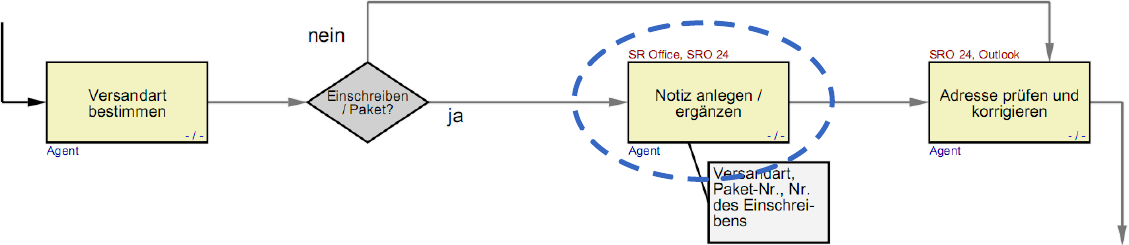
\includegraphics[width=15cm]{ipm-process.png}
\caption{Perspektivenorientierte Prozessmodellierung aus \cite{roth_konzeption_2011}}\label{grundlagen:ipm-process}\end{figure}


\subsection{Grafische Modellierungswerkzeuge}
\label{grundlagen:modellierungswerkzeuge}\label{grundlagen:grafische-modellierungswerkzeuge}
Für die Erstellung von grafischen Prozessmodellen am Rechner wird eine Unterstützung durch Softwarewerkzeuge benötigt.
Prinzipiell können "`Modelle"' einfach mit Hilfe von 2D-Zeichenwerkzeugen wie \emph{Dia} \cite{www:dia} oder \emph{MS Visio} \cite{www:visio} erstellt werden.
Solche Programme bieten oft schon passende Formen und Verbindungen, beispielsweise für BPMN\footnote{
Business Process Modeling and Notation; umfasst eine standardisierte, (grafische) Prozessmodellierungssprache. Siehe \cite{www:bpmn}.
} an.
Ein Benutzer macht die Bedeutung eines solchen Diagramms an den erkennbaren grafischen Formen und deren Aussehen fest; insofern wäre dies für Menschen durchaus ausreichend.

Durch ein Zeichenprogramm wird das Diagramm intern nur als eine Ansammlung von Bildpunkten oder geometrischen Primitiven dargestellt und auch entsprechend gespeichert ("`persistiert"').
Für ein solches Programm hat die Semantik der grafischen Konstrukte keinerlei Bedeutung.
So ergibt sich ein Problem, wenn der modellierte Prozess automatisch ausgeführt oder verändert werden soll.
Wie soll den grafischen Elementen eine Bedeutung zugeordnet werden?

Daher sind eher Werkzeuge gefragt, die auch intern eine "`Vorstellung"' von Modellierungskonzepten haben \cite{volz_werkzeugunterstutzung_2011}.
Solche Werkzeuge werden – auch in dieser Arbeit – "'Modellierungswerkzeuge"' genannt.

Ein solches grafisches Werkzeug bietet die Möglichkeit, Modelle zu erstellen, diese in formaler Weise zu persistieren und wieder aus einer physischen Repräsentation – beispielsweise einer Datei – zu laden.
Dem Benutzer wird üblicherweise eine Palette an Modellelementen angeboten, die in einem konkreten Prozessmodell eingesetzt werden können.
Ein Anwender "`baut"' ein Modell, indem er Instanzen der grafischen Objekte miteinander auf einer "`Zeichenfläche"' kombiniert.
Zu den konkreten, grafischen Elementen wird automatisch eine abstrakte Instanz angelegt, welche die Bedeutung des Modellelements festlegt.

Änderungen am abstrakten Modellelement können die Darstellung der grafischen Elemente beeinflussen.
So kann beispielsweise in einem Prozessknoten dessen Funktion angegeben sein, welche in der grafischen Repräsentation als Text angezeigt wird.
Bei einer Änderung der Funktion im Modellelement wird auch der Text auf dem Grafikobjekt angepasst.
Genauso können Eigenschaften oder der Typ eines Modellelements durch Symbole auf den Grafikobjekten visualisiert werden.

Ein Modellierungswerkzeug für die perspektivenorientierte Prozessmodellierung wird in \hyperref[grundlagen:ipm2]{Abbildung  \ref*{grundlagen:ipm2}} gezeigt.
Auf der linken Seite lässt sich die Palette mit den Modellelementen erkennen, die in verschiedene "`Gruppen"' eingeordnet sind.
\begin{figure}[htbp]
\centering
\capstart

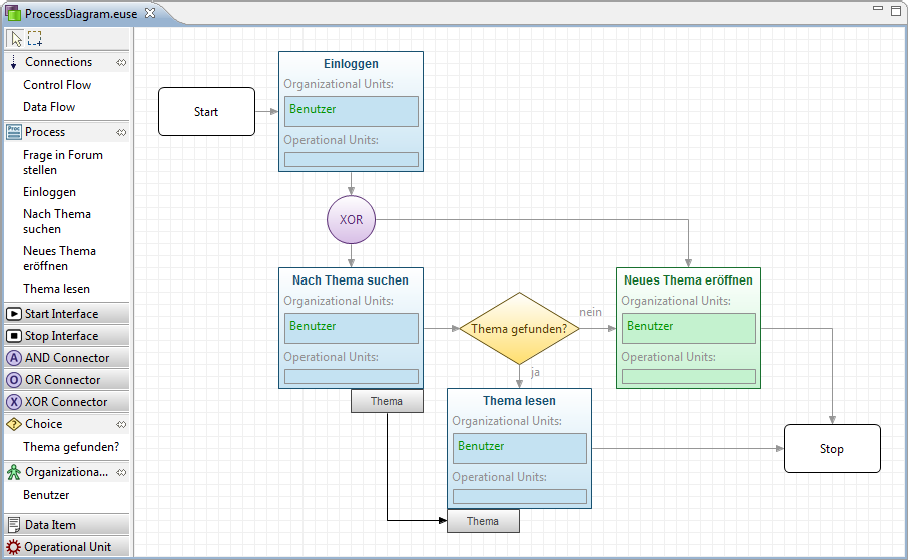
\includegraphics[width=15cm]{ipm2d-editor.png}
\caption{Prozessmodellierungswerkzeug i\textgreater{}PM2 aus \cite{roth_konzeption_2011}}\label{grundlagen:ipm2}\end{figure}


\section{Metamodellierung}
\label{grundlagen:id5}\label{grundlagen:metamodellierung}
In der Prozessmodellierung kann es sinnvoll sein, die Modellierungssprache selbst zu verändern, um diese an spezielle Anforderungen anzupassen.
So lassen sich Sachverhalte verständlicher und direkter als mit allgemeinen, fest vordefinierten Sprachen darstellen, indem spezialisierte Sprachelemente verwendet werden.
An ein bestimmtes Einsatzgebiet angepasste Sprachen werden als \textbf{domänenspezifische Sprachen} (DSL) bezeichnet \cite{clark_applied_2008}.

Zur Beschreibung von Modellierungssprachen lässt sich das Konzept der \textbf{Metamodellierung} einsetzen \cite{weisemoller_comparison_2008} \cite{volz_werkzeugunterstutzung_2011}.
Ein Metamodell lässt sich als ein Modell für eine Menge ("`Klasse"') von Modellen charakterisieren \cite{seidewitz_what_2003}.

Durch die Anpassung eines Metamodells, welches die abstrakte Syntax beschreibt, können neue Modellelemente hinzugefügt und bestehende angepasst oder entfernt werden.
Andererseits lässt sich die konkrete Syntax, im Falle einer grafischen Sprache also die grafische Repräsentation der Modellelemente ebenfalls durch ein Metamodell spezifizieren.
So ist es möglich, zu einer abstrakten Syntax mehrere grafische Repräsentationen zu erstellen, die auf spezielle Anforderungen zugeschnitten sein können \cite{jablonski_perspective_2008}.

Um Metamodelle zu "`erstellen"' ist es notwendig, diese auf eine wohldefinierte Weise beschreiben zu können.
Dies leistet das im Folgenden vorgestellte Linguistic Meta Model (LMM), welches im Rahmen des Open Meta Modelling Environment (OMME), einer Metamodellierungsumgebung, entstanden ist \cite{volz_werkzeugunterstutzung_2011}.


\subsection{Linguistic Meta Model}
\label{grundlagen:lmm}\label{grundlagen:linguistic-meta-model}
LMM stellt eine Sprache bereit, welche zur Definition von Metamodellen dient.
\hyperref[grundlagen:lmm-model]{Abbildung  \ref*{grundlagen:lmm-model}} zeigt die grundlegenden LMM-Elemente und deren Hierarchie.
\begin{figure}[htbp]
\centering
\capstart

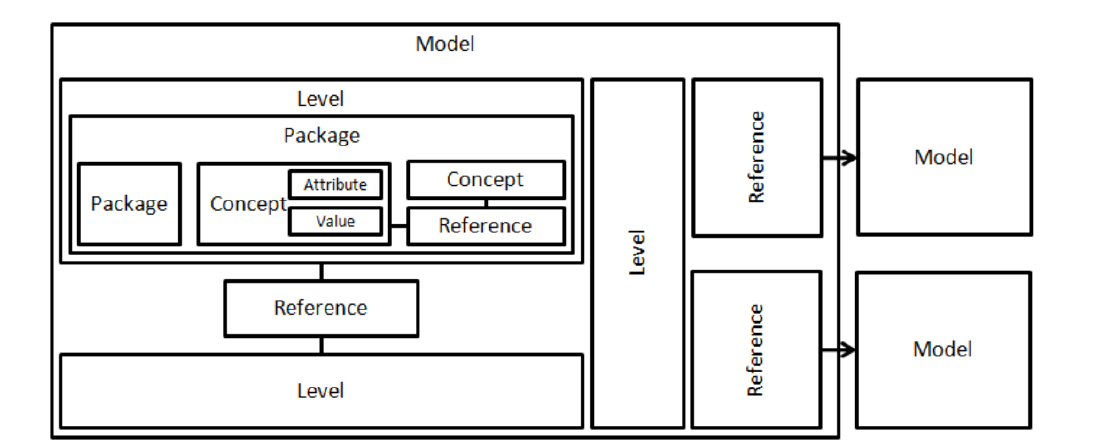
\includegraphics[width=14cm]{bernhard-lmmmodel.png}
\caption{Hierarchie der LMM-Elemente aus \cite{volz_werkzeugunterstutzung_2011}}\label{grundlagen:lmm-model}\end{figure}

Das zentrale Element im LMM ist das \textbf{Concept}.

Ein Concept kombiniert Eigenschaften einer Klasse und eines Objekts, wie sie aus objektorientierten Programmiersprachen\footnote{
Dies deckt natürlich nicht alle objektorientierten Programmiersprachen ab. "`Objektorientierung"' kann durchaus auf anderem Wege umgesetzt werden.
} bekannt sind.
So kann ein Concept – wie eine Klasse – Attribute definieren. Gleichzeitig kann ein Concept – wie ein Objekt –  Wertzuweisungen enthalten.
Anders ausgedrückt können Concepts sowohl eine "`Typ-Facette"', die Attribute definiert als auch eine "`Instanz-Facette"', die Zuweisungen vornimmt, beinhalten \cite{atkinson_meta-level_2000}.
Dieses Prinzip wird mit dem Begriff \textbf{Clabject} (\textbf{Cla}ss and O\textbf{bject}) umschrieben.

Klassen stellen im objektorientierten System Typen dar; Objekte sind Instanzen von Klassen, welche Werte an die Attribute der Klasse zuweisen.
Im Gegensatz zu der von Klasse und Objekt vorgegebenen Hierarchie aus zwei "`Ebenen"' lassen sich mit Concepts Hierarchien mit beliebig vielen Ebenen realisieren.
Dazu können Concepts gleichzeitig den Typ für Concepts auf der darunterliegenden Ebene und eine Instanz eines Concepts (\code{instanceOf}) auf der nächsthöheren Ebene darstellen.
Ebenso gibt es die Möglichkeit für Concepts, andere Concepts analog zu Klassen zu "`erweitern"' (\code{extends}), also einen Subtyp zu bilden.

Ein Vergleich zwischen Klasse-Objekt-Beziehungen und Concept-Concept-Beziehungen  ist in \hyperref[grundlagen:vergleich-lmm]{Abbildung  \ref*{grundlagen:vergleich-lmm}} zu sehen.
In der Abbildung besitzt \code{ConceptC} eine Instanz-Facette, welche den Attributen aus \code{ConceptA} und \code{ConceptB} Werte zuweist.
Die Typ-Facette von \code{ConceptC} stellt das Attribut \code{c} bereit, welches von \code{ConceptD} mit dem Wert 5.5 belegt wird.
\begin{figure}[htbp]
\centering
\capstart

\includegraphics[width=17cm]{vergleich_lmm.eps}
\caption{Vergleich von objektorientierter Modellierung (links) und Metamodellierung mit Clabjects}\label{grundlagen:vergleich-lmm}\end{figure}

Concepts werden, wie in \hyperref[grundlagen:lmm-model]{Abbildung  \ref*{grundlagen:lmm-model}} gezeigt, in \textbf{Packages} eingeordnet. Packages bilden zusammen einen \textbf{Level}, welcher eine Ebene in der Metamodellierungshierarchie repräsentiert.
Mehrere Levels stellen zusammen das vollständige \textbf{Model} dar, wobei auch Modelle mit nur einer Ebene erlaubt sind.

Levels können ebenfalls zueinander in einer Instanzbeziehung (\code{instanceOf}) stehen.
Wenn alle in einem Level \emph{MA} definierten Concepts Instanzen von jeweils genau einem Concept in Level \emph{MB} sind, ist \emph{MA} eine Instanz von \emph{MB},

Die genannten Beziehungen wie \code{instanceOf} zwischen Levels bzw. Concepts werden in \hyperref[grundlagen:lmm-model]{Abbildung  \ref*{grundlagen:lmm-model}} als "`Reference"' dargestellt.
In Concepts können sowohl \textbf{Literaltyp-Attribute} (bspw. string, real, integer) als auch \textbf{Referenz-Attribute}, welche auf andere Concepts verweisen, angegeben werden.

Neben der schon erwähnten Instanziierung und Subtypbildung werden von LMM zusätzliche Modellierungsmuster unterstützt.
Von diesen ist für die vorliegende Arbeit die sog. \textbf{Spezialisierung von Instanzen}  bedeutend, deren Vorteile für die Modellierung von \cite{volz_werkzeugunterstutzung_2011} beschrieben werden.
Dieses Muster wird in \hyperref[grundlagen:concreteuseof]{Abbildung  \ref*{grundlagen:concreteuseof}} veranschaulicht.
\begin{figure}[htbp]
\centering
\capstart

\includegraphics[width=15.5cm]{concreteuseof.eps}
\caption{Instanz-Spezialisierung ausgehend von ConceptD}\label{grundlagen:concreteuseof}\end{figure}

In der Abbildung spezialisiert \code{UseA} \code{ConceptD} (\code{concreteUseOf}). \code{UseA} übernimmt dabei alle Zuweisungen von \code{ConceptD}; damit hat das Attribut in \code{UseA} ebenfalls den Wert 5.5.
\code{UseB} dagegen setzt wiederum einen Wert für das Attribut \code{c}. Das heißt, dass in \code{UseB} die bisherige Zuweisung "`überschrieben"' wird und damit den Wert 0 hat.
Für \code{ConceptD} ändert sich dabei nichts; die Überschreibung wirkt sich nur in \code{UseB} aus.
In LMM lässt sich für Attribute festlegen, inwieweit das Setzen von Werten in Spezialisierungen zulässig ist und welche Bedeutung dies hat.

LMM-(Meta-)Modelle lassen sich mit der Sprache Linguistic Meta Language (LML) \cite{volz_werkzeugunterstutzung_2011} (S.159ff) in einer textuellen Form beschreiben.
Die Syntax ist an bekannte Programmiersprachen wie C++ oder C\# angelehnt und kann daher als "`menschenlesbar"' angesehen werden.
Gleichzeitig ist es damit möglich, LMM automatisch zu verarbeiten oder es sogar für die Beschreibung von Software zu nutzen, wie im Folgenden am Beispiel des MDF gezeigt wird.

Beispielsweise sieht ein Concept mit einer Zuweisung und einer Attributdefinition in LML wie folgt aus:

\begin{Verbatim}[commandchars=\\\{\}]
\PYG{n}{concept} \PYG{n}{ConceptC} \PYG{n}{instanceOf} \PYG{n}{ConceptB} \PYG{o}{\PYGZob{}}
    \PYG{n}{a} \PYG{o}{=} \PYG{l+m+mi}{7}\PYG{o}{;}
    \PYG{n}{real} \PYG{n}{c}\PYG{o}{;}
\PYG{o}{\PYGZcb{}}
\end{Verbatim}

Zur einfachen Bearbeitung von LMM-Modellen wird von OMME ein textueller Editor auf Basis von Xtext \cite{www:xtext} bereitgestellt.


\subsection{Model Designer Framework}
\label{grundlagen:model-designer-framework}\label{grundlagen:mdf}
Ebenfalls als Teil der Metamodellierungsumgebung OMME ist das Model Designer Framework (MDF) von Roth \cite{roth_konzeption_2011} entwickelt worden.
Dieses erlaubt es, Modell-Editoren mit Hilfe von LMM-Metamodellen zu spezifizieren.
So lassen sich grafische Modellierungswerkzeuge ("`Editoren"') auf Basis von MDF für beliebige (domänenspezifische) Modellierungssprachen erstellen.

\hyperref[grundlagen:mdf-modellhierarchie]{Abbildung  \ref*{grundlagen:mdf-modellhierarchie}} zeigt die in MDF verwendeten Modelle. Hier sollen nur kurz die für die vorliegende Arbeit wichtigsten Aspekte verdeutlicht werden.
Details können bei Roth in Kapitel 5, Modellhierarchie nachgelesen werden.
\begin{figure}[htbp]
\centering
\capstart

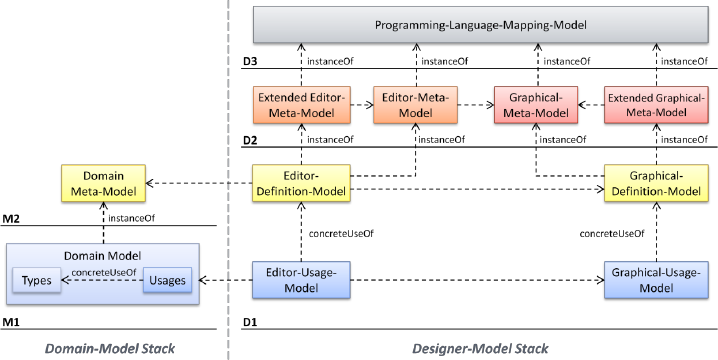
\includegraphics[width=15cm]{mdf-modellhierarchie.png}
\caption{Modellhierarchie von MDF mit Domain-Model- und Designer-Stack aus \cite{roth_konzeption_2011}}\label{grundlagen:mdf-modellhierarchie}\end{figure}

Der \emph{Domain-Model-Stack} (links) enthält alle Modelle, die für die Domäne relevant sind.
Das \emph{Domain-Metamodel} legt die Elemente der domänenspezifischen Sprache fest, welche im \emph{Domain-Model} genutzt wird, um ein Modell zu beschreiben.

Rechts wird der \emph{Designer-Model-Stack} gezeigt, der den Editor für die Domäne spezifiziert.
Das \emph{Graphical-Definition-Model} beschreibt Figuren, die sich für die Visualisierung der Domäne einsetzen lassen.
Figuren werden über das \emph{Editor-Definition-Model} mit den Domänenmodellelementen verbunden. So wird die grafische Repräsentation der Modellelemente im Editor festgelegt.
Bemerkenswert ist, dass LMM sowohl für die Beschreibung des Modellierungswerkzeugs als auch für die persistente Speicherung und interne Darstellung der mit dem Werkzeug erstellten Modelle genutzt wird.

\hyperref[grundlagen:ipm-typ-verwendung-2]{Abbildung  \ref*{grundlagen:ipm-typ-verwendung-2}} zeigt einen Prozess, der in einem mit MDF definierten Editor (\emph{i\textgreater{}PM}$^{\text{2}}$) für die {\hyperref[grundlagen:popm]{\emph{POPM}}} (\autoref*{grundlagen:popm}) erstellt wurde.


\section{Typ-Verwendungs-Konzept}
\label{grundlagen:typ-verwendungs-konzept}\label{grundlagen:tvk}
An \hyperref[grundlagen:ipm-typ-verwendung-1]{Abbildung  \ref*{grundlagen:ipm-typ-verwendung-1}} und \hyperref[grundlagen:ipm-typ-verwendung-2]{Abbildung  \ref*{grundlagen:ipm-typ-verwendung-2}} lässt sich das "`Typ-Verwendungs-Konzept"', welches von i\textgreater{}PM$^{\text{2}}$ umgesetzt wird, zeigen.

Das Grundprinzip des Typ-Verwendungs-Konzeptes ist es, einmal erstellte Objekte in unterschiedlichen Zusammenhängen zu verwenden.
Dieses Konzept lässt sich durch die in {\hyperref[grundlagen:lmm]{\emph{LMM}}} (\autoref*{grundlagen:lmm}) eingeführte Spezialisierung von Instanzen leicht realisieren\footnote{
Nach der Terminologie des Typ-Verwendungs-Konzepts ist in der \hyperref[grundlagen:concreteuseof]{Abbildung  \ref*{grundlagen:concreteuseof}} \code{ConceptD} ein "`Typ"', \code{UseA} und \code{UseB} sind "`Verwendungen"' davon.
}.
Die Spezialisierung von Instanzen, deren Einsatz für das Typ-Verwendungs-Konzept und das im Folgenden gezeigte Beispiel werden auch in der Arbeit von Volz \cite{volz_werkzeugunterstutzung_2011} (S.56ff) beschrieben.

\hyperref[grundlagen:ipm-typ-verwendung-1]{Abbildung  \ref*{grundlagen:ipm-typ-verwendung-1}} zeigt den Prozess "`Notiz aufnehmen"' (\emph{A}).
Nun wird eine sehr ähnliche Funktionalität für einen anderen Prozess benötigt, der in \hyperref[grundlagen:ipm-typ-verwendung-2]{Abbildung  \ref*{grundlagen:ipm-typ-verwendung-2}} gezeigt ist.
Hier ist der Prozess "`Notiz erstellen / ergänzen"' (\emph{B}) zu sehen.
Um diesen Prozess zu definieren, könnte nun ein komplett neues "`Objekt"' erstellt werden.
Es ist allerdings schon ein "`Objekt"' mit nahezu gleichen Eigenschaften vorhanden, nämlich der vorher genannte Prozess \emph{A}.
Wie in der Informatik üblich wäre es wünschenswert, solche Redundanzen zu vermeiden und die "`Wiederverwendbarkeit"' zu erhöhen.

Dazu kann ein "`Typ"' definiert werden, vom dem mehrere "`Verwendungen"' erstellt werden, die dann in mehreren Kontexten eingesetzt werden können.
Hier könnte beispielsweise der Typ \emph{T} angelegt werden, welcher einen Prozess repräsentiert.
\emph{T} legt fest, dass die Funktion des Prozesses "`Notiz aufnehmen"' (der auf der Figur angezeigte Text) ist und "`OneNote"' und "`Agent"' mit ihm assoziiert sind.
Prozess \emph{A} kann als Verwendung von \emph{T} gesehen werden; \emph{A} übernimmt alle Eigenschaften von \emph{T}.

Um den Prozess \emph{B} darzustellen, müssen jedoch zwei Änderungen vorgenommen werden.
Das ist möglich, da eine Verwendung Werte des Typs überschreiben kann.
So wird in der Verwendung für \emph{B} die vordefinierte Funktion durch "`Notiz erstellen / ergänzen"' ersetzt und "`Outlook"' zu den operationalen Einheiten hinzugefügt.
\begin{figure}[htbp]
\centering
\capstart

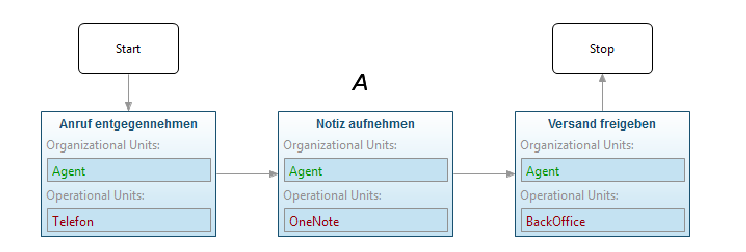
\includegraphics{ipm2-typ-verwendung_2.png}
\caption{Prozess in i\textgreater{}PM2 aus \cite{volz_werkzeugunterstutzung_2011} (Bezeichner A hinzugefügt)}\label{grundlagen:ipm-typ-verwendung-1}\end{figure}
\begin{figure}[htbp]
\centering
\capstart

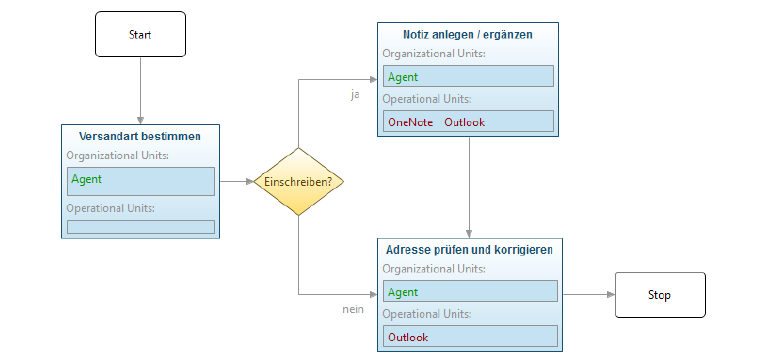
\includegraphics{ipm2-typ-verwendung_1.png}
\caption{Prozess mit angepasster Verwendung aus \cite{volz_werkzeugunterstutzung_2011} (B hinzugefügt)}\label{grundlagen:ipm-typ-verwendung-2}\end{figure}

Das Typ-Verwendungs-Konzept ist auch in i\textgreater{}PM$^{\text{2}}$ (\hyperref[grundlagen:ipm2]{Abbildung  \ref*{grundlagen:ipm2}}) zu erkennen.
Die Palette (links) zeigt unter "`Process"' die davon instanziierten "`Typen"', wovon für die Zeichenfläche "`Verwendungen"' erstellt werden.
Rechts auf der Zeichenfläche ist eine Verwendung vom Typ "`Neues Thema eröffnen"' mit geänderter Grundfarbe zu sehen.


\chapter{Verwandte Arbeiten zur 3D-Visualisierung}
\label{related:verwandte-arbeiten-zur-3d-visualisierung}\label{related::doc}\label{related:related}
Neben den (wenigen) Arbeiten, die sich explizit mit der dreidimensionalen Visualisierung und Modellierung von Prozessen beschäftigen, sollen hier auch solche vorgestellt werden, die sich allgemein oder in verwandten Gebieten wie der Softwaremodellierung mit 3D-Visualisierungen beschäftigen.

Die hier gezeigten Arbeiten sollen als Anregung oder Motivation für die in dieser Arbeit dargestellte 3D-Visualisierung von Prozessen dienen.
Außerdem sollen Ideen für zukünftige Erweiterungen des vorliegenden Projekts gesammelt und prinzipielle Vor- und Nachteile von 3D-Visualisierungen beleuchtet werden.


\section{3D-Softwarevisualisierung}
\label{related:d-softwarevisualisierung}
Nahe verwandt mit der Prozessmodellierung ist die Modellierung von Software.
Nicht selten sind Softwaresysteme überaus umfangreich und es muss daher nach Möglichkeiten gesucht werden, eine Vielzahl von Informationen übersichtlich und klar zu visualisieren ohne den Betrachter zu überfordern.

Bisher nutzen Werkzeuge zur Softwaremodellierung, die häufig auf der Unified Modeling Language (UML) aufsetzen nahezu ausschließlich 2D-Visualisierungen.
Die UML lässt prinzipiell aber auch 3D-Repräsentationen zu \cite{booch_unified_1999}.
Einen umfassenden Überblick über Arbeiten, die sich mit 3D-Softwarevisualisierung befassen, gibt \cite{teyseyre_overview_2009}.


\subsection{Wilma: Ein 3D-Modellierungstool für UML-Diagramme}
\label{related:dywer}\label{related:wilma-ein-3d-modellierungstool-fur-uml-diagramme}
\cite{dwyer_three_2001} weist auf die Probleme von Softwarevisualisierungstechniken hin, große und insbesondere hierarchisch aufgebaute Diagramme darzustellen.
3D-Darstellungen hätten hier Vorteile durch die Möglichkeit, Hierarchieebenen des Diagramms als Flächen im 3D-Raum zu zeigen.

Die Platzierung von UML-Elementen per Hand sei eine zeitraubende Aufgabe, die besonders im dreidimensionalen Raum wegen der schlechten Verfügbarkeit von 3D-Eingabegeräten zum Problem werde.
Daher wird eine Anordnung der Diagrammelemente im 3D-Raum mit Hilfe eines automatischen, kräftebasierten Layout-Algorithmus vorgeschlagen.

Es wurde ein Prototyp ("`Wilma"')\footnote{
Quellcode und ausführbare Dateien des (weiterentwickelten) Prototyps "`WilmaScope"' (auf Basis von Java3D) können unter \href{http://wilma.sourceforge.net/}{http://wilma.sourceforge.net/} heruntergeladen werden.
} realisiert, der Graphen in einer 3D-Darstellung zeichnen kann und Interaktionsmöglichkeiten mit den Graphelementen bietet.
Ein damit erstelltes 3D-Klassendiagramm ist in \hyperref[related:dywer-classdiag]{Abbildung  \ref*{related:dywer-classdiag}} zu sehen.

So werden Klassen durch 3D-Quader dargestellt, deren Seiten beschriftet werden können.
Um die Lesbarkeit sicherzustellen, wird immer eine Seite des Würfels auf den Betrachter ausgerichtet.
Pakete werden durch transluzente Kugeln und Verbindungen zwischen Klassen durch gestreckte 3D-Zylinder dargestellt.
\begin{figure}[htbp]
\centering
\capstart

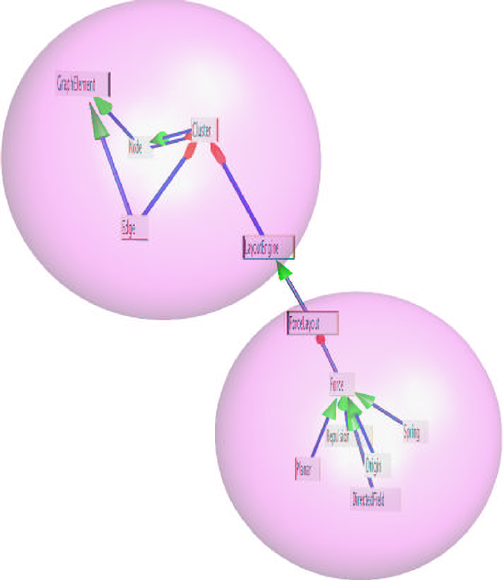
\includegraphics[height=15cm]{dywer_classdiag.png}
\caption{3D-UML-Klassendiagramm aus \cite{dwyer_three_2001}}\label{related:dywer-classdiag}\end{figure}

In einer Studie zur Benutzbarkeit seien die 3D-Diagramme von Beteiligten als nützlich für das Verständnis des Modells eingestuft worden.
Es wird ein Benutzer zitiert, der die Möglichkeit, das Diagramm aus verschiedenen Richtungen betrachten zu können besonders positiv kommentiert.

Auch seien Benutzer gebeten worden, selbst ein 3D-Diagramm nach einer textuellen Vorlage zu modellieren, wobei die meisten wenig Probleme mit der Aufgabe gehabt hätten.
Es wird jedoch vermutet, dass die 3D-Darstellung bei einigen Benutzern eine gewisse Eingewöhnungszeit voraussetzen könnte.
Probanden mit vorheriger Erfahrung aus 3D-Computerspielen hätten im Versuch die wenigsten Schwierigkeiten mit der Navigation im 3D-Raum gehabt.


\subsection{X3D-UML: Hierarchische 3D-UML-Zustandsdiagramme}
\label{related:x3d-uml-hierarchische-3d-uml-zustandsdiagramme}\label{related:mcintosh}
In \cite{mcintosh_x3d-uml:_2008} werden Zustandsdiagramme ("`state diagrams"') der UML in den 3D-Raum übertragen.

Zu Beginn seien von vier Unternehmen erhaltene Zustandsdiagramme untersucht worden, die mit dem Modellierungswerkzeug IBM Rational Rose erstellt wurden.
Daraus habe sich ergeben, dass die Modelle oft hierarchisch aus Unterzuständen aufgebaut seien.
In RationalRose würden diese Unterdiagramme jedoch in separaten Tabs dargestellt, was dazu führe, dass Betrachter ständig zwischen einzelnen Diagrammen hin- und herwechseln müssten.
Das erschwere das Erkennen von Zusammenhängen und groben Strukturen, was von befragten Benutzern bemängelt worden sei.
Die Einschränkungen durch die Tab-Ansicht würden auf verschiedenem Wege "`umgangen"', etwa indem separate Handskizzen angefertigt würden.
Andere Benutzer würden "`in die Luft starren"', um sich die Zusammenhänge und Auswirkungen von Änderungen besser vorstellen zu können.

Daher sei es die wichtigste Anforderung an eine 3D-Repräsentation, hier Abhilfe zu schaffen und hierarchische Zustandsdiagramme besser abzubilden.
Es wird eine Darstellung vorgeschlagen, welche die Zustandsdiagramme selbst immer noch zweidimensional zeichnet, diese jedoch auf ebenen Flächen im 3D-Raum platziert.
So würden sich Beziehungen zwischen mehreren Diagrammen gut grafisch darstellen lassen.
Wie sich in \hyperref[related:mcintosh-sm]{Abbildung  \ref*{related:mcintosh-sm}} erkennen lässt, werden Beziehungen zwischen Super- und Subzuständen durch transluzente, graues Dreiecke dargestellt.

Solche Diagramme seien Benutzern mit Erfahrung in Rational Rose vorgelegt worden, welche sich insgesamt positiv zur Nützlichkeit jener 3D-Diagramme geäußert hätten.
Von den Benutzern seien verschiedene Erweiterungen vorgeschlagen worden; unter anderem eine Filtermöglichkeit, mit der sich uninteressante Details verbergen lassen, Einschränkungen der Navigation um ungünstige Sichten auf das Modell zu vermeiden (bspw. direkt von der Seite, so dass die 2D-Elemente nicht erkennbar sind) sowie Funktionen, um schnell zwischen verschiedenen Betrachtungsperspektiven wechseln zu können.
\begin{figure}[htbp]
\centering
\capstart

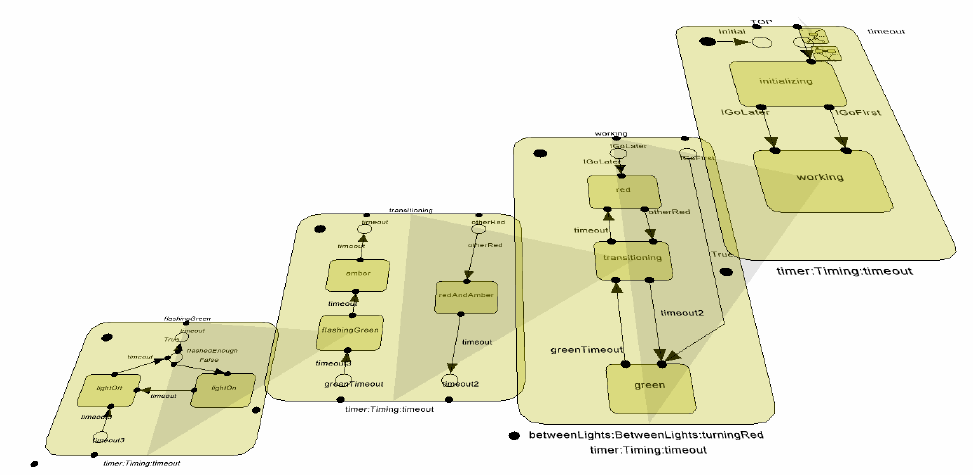
\includegraphics[width=16.5cm]{mcintosh_sm.png}
\caption{Hierarchisch aufgebautes 3D-UML-Zustandsdiagramm aus \cite{mcintosh_x3d-uml:_2008}}\label{related:mcintosh-sm}\end{figure}
\pagebreak

\subsection{3D-Visualisierung von großen, hierarchischen UML-Zustandsdiagrammen}
\label{related:d-visualisierung-von-groszen-hierarchischen-uml-zustandsdiagrammen}\label{related:krolovitsch}
3D-Visualisierungen von (großen) UML-Zustandsdiagrammen werden auch von \cite{krolovitsch_3d_2009} und, darauf aufbauend, \cite{alvergren_3d_2009} untersucht.
Zustandsdiagramme werden, wie in \cite{mcintosh_x3d-uml:_2008} auf Flächen im 3D-Raum gezeichnet, wobei hier die Zustände selbst als 3D-Objekte dargestellt sind, um den visuellen Eindruck zu verbessern, wie in \hyperref[related:krolovitsch-sm]{Abbildung  \ref*{related:krolovitsch-sm}} zu sehen ist.

\hyperref[related:krolovitsch-sm-nodes]{Abbildung  \ref*{related:krolovitsch-sm-nodes}} zeigt, wie in komplexen Diagrammen komplette Diagrammteile ausgeblendet und durch einen blauen Würfel ersetzt werden können, um momentan unwichtige Details zu verbergen und die Übersichtlichkeit zu erhöhen.
\begin{figure}[htbp]
\centering
\capstart

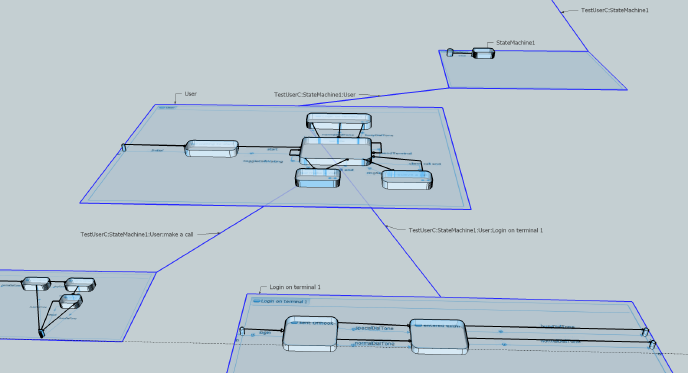
\includegraphics[width=15.5cm]{krolovitsch_sm.png}
\caption{3D-Zustandsdiagramm aus \cite{krolovitsch_3d_2009}}\label{related:krolovitsch-sm}\end{figure}
\begin{figure}[htbp]
\centering
\capstart

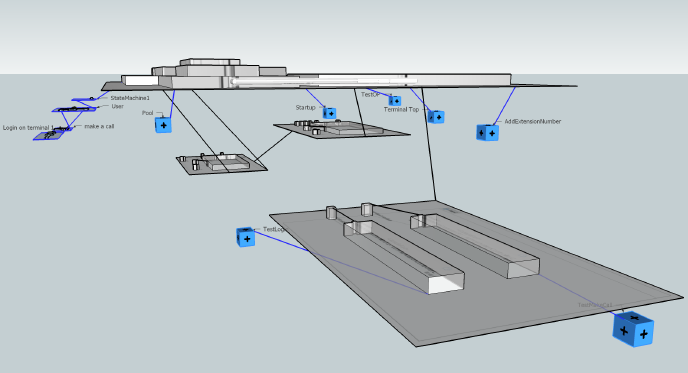
\includegraphics[width=15.5cm]{krolovitsch_sm_nodes.png}
\caption{Zustandsdiagramm mit ausgeblendeten Diagrammteilen (dargestellt durch blaue Würfel) aus \cite{krolovitsch_3d_2009}}\label{related:krolovitsch-sm-nodes}\end{figure}


\subsection{Dreidimensionale Darstellung zur besseren Visualisierung von Beziehungen}
\label{related:gil}\label{related:dreidimensionale-darstellung-zur-besseren-visualisierung-von-beziehungen}
\cite{gil_three_1998} merkt an, dass durch 3D-Visualisierungen die Ausdrucksstärke von (graphbasierten) grafischen Notationen deutlich erhöht werden könne.
Besonders vorteilhaft seien 3D-Visualisierungen von Graphen, wenn es darum ginge, eine Vielzahl von unterschiedlichen Beziehungs- bzw. Verbindungstypen darzustellen.
Im 2D-Bereich habe man nur relativ eingeschränkte Möglichkeiten, unterschiedliche Verbindungstypen durch Farbe, unterschiedliche Linentypen oder durch Konnektoren – Symbole an den Enden der Linien – voneinander abzugrenzen.
Um diese Probleme im 2D-Raum zu umgehen würden oft unterschiedliche Graphen bzw. Diagrammtypen genutzt.
Dabei besäßen Knoten in unterschiedlichen Diagrammtypen oft die gleiche Bedeutung während Verbindungen eine komplett andere Semantik hätten.
Problematisch sei die Repräsentation von Zusammenhängen zwischen unterschiedlichen Diagrammtypen, was allgemein einen großen Schwachpunkt von Modellierungssprachen darstelle.

Zur Visualisierung von Verbindungen lasse sich die dritte Dimension, also die z-Richtung sinnvoll nutzen.
Verbindungen in der x-y-Ebene hätten eine andere Bedeutung als die, die aus der Ebene heraus in z-Richtung verlaufen. So würden sich mehrere Diagrammtypen in eine Darstellung integrieren lassen.

Die dritte Dimension ließe sich auch als Zeitachse interpretieren.
So sei es möglich, in 3D-Sequenzdiagrammen die Zustände des Systems zu bestimmten Zeitpunkten auf parallelen Flächen darzustellen, zu denen die Zeitachse senkrecht steht wie in \hyperref[related:gil-sequencediag]{Abbildung  \ref*{related:gil-sequencediag}} gezeigt wird.
\begin{figure}[htbp]
\centering
\capstart

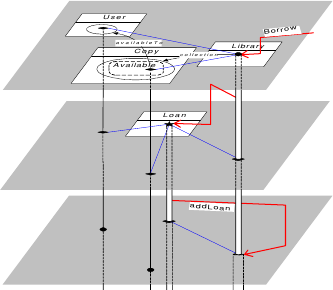
\includegraphics[height=7cm]{gil_sequencediag.png}
\caption{3D-UML-Sequenzdiagramm; Ausschnitt aus \cite{gil_three_1998}}\label{related:gil-sequencediag}\end{figure}


\subsection{Nutzung von Tiefeneindruck und Animation zur Visualisierung von UML-Diagrammen}
\label{related:gogolla}\label{related:nutzung-von-tiefeneindruck-und-animation-zur-visualisierung-von-uml-diagrammen}
In \cite{gogolla_towards_1999} wird ebenfalls die 3D-Darstellung von UML-Diagrammen, speziell Klassen-, Objekt- und Sequenzdiagrammen untersucht.
Die dritte Dimension könne beispielsweise dafür genutzt werden, als "`uninteressant"' eingestufte Elemente in den Hintergrund zu schieben und damit Elemente im Vordergrund besonders hervorzuheben.

In \hyperref[related:gogolla-classdiag-a]{Abbildung  \ref*{related:gogolla-classdiag-a}} und \hyperref[related:gogolla-classdiag-b]{Abbildung  \ref*{related:gogolla-classdiag-b}} wird das Prinzip am Beispiel eines Klassendiagramms verdeutlicht.
Bei letzerer Abbildung ist zu sehen, dass bei Klassen, die nah am Betrachter sind, mehr Information dargestellt wird als bei den in größerer Entfernung dargestellten Klassen, bei denen nur der Name als Text zu erkennen ist.
Zusätzlich wird die Nutzung von Animationen vorgeschlagen, um Übergänge zwischen verschiedenen Visualisierungsperspektiven – wie zwischen den beiden gezeigten Abbildungen – anschaulicher zu machen.
\begin{figure}[htbp]
\centering
\capstart

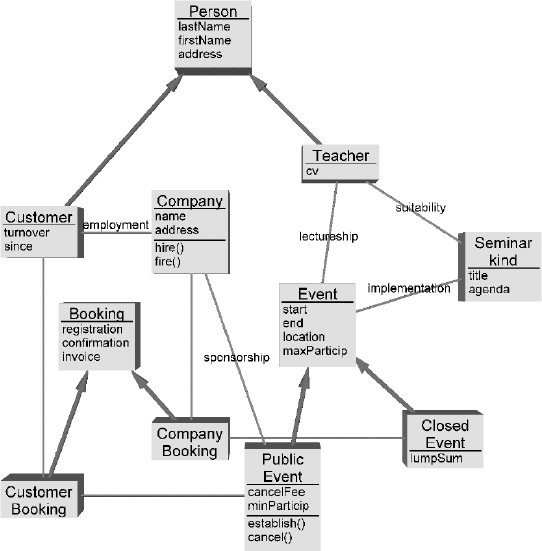
\includegraphics[height=9cm]{gogolla_classdiag_a.png}
\caption{3D-UML-Klassendiagramm aus \cite{gogolla_towards_1999}}\label{related:gogolla-classdiag-a}\end{figure}
\begin{figure}[htbp]
\centering
\capstart

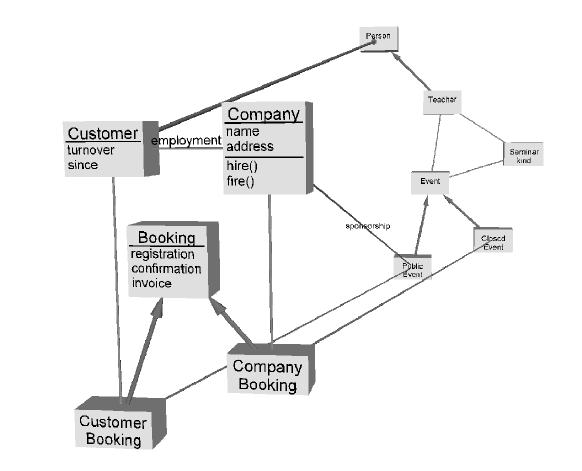
\includegraphics[height=9cm]{gogolla_classdiag_b.png}
\caption{Diagramm mit nach hinten verschobenen, "`unwichtigen"' Klassen aus \cite{gogolla_towards_1999}}\label{related:gogolla-classdiag-b}\end{figure}


\subsection{Graphical Editing Framework 3D}
\label{related:gef3d}\label{related:graphical-editing-framework-3d}
Bei GEF3D handelt es sich um ein Framework zur Erstellung von Modell-Editoren \cite{von_pilgrim_gef3d:_2008}.
Das Projekt basiert auf den Konzepten des Grafical Editing Framework der Eclipse Plattform und überträgt diese in den dreidimensionalen Raum.

Mit GEF3D ist es möglich, 3D-Editoren für Eclipse zu erstellen und schon vorhandene, GEF-basierte 2D-Editoren darin einzubetten indem 2D-Elemente auf Flächen im dreidimensionalen Raum gezeichnet würden.
\hyperref[related:gef3d-twt3d]{Abbildung  \ref*{related:gef3d-twt3d}} zeigt ein Beispiel für die Darstellung von mehreren Diagrammtypen in einer Ansicht und Verbindungen zwischen Elementen verschiedener Diagramme.

In \hyperref[related:gef3d-ecore]{Abbildung  \ref*{related:gef3d-ecore}} ist ein mit GEF3D implementierter Ecore-Editor zu sehen.
Diese Darstellungsform mit 2D-Elementen, die im 3D-Raum platziert werden können wird als "`2.5D"'-Darstellung bezeichnet.
Elemente könnten, wie in der Abbildung zu sehen ist, auf Flächen oder auch frei im 3D-Raum platziert werden \cite{www:gef3ddevblog}.

Die grafische Ausgabe von GEF3D baut direkt auf OpenGL auf; um 2D-Grafiken und Text zu zeichnen werde Vektorgrafik genutzt, was zu einer besseren Darstellungsqualität im Vergleich zu texturbasiertem 2D-Rendering führe\footnote{
Ein verbreiteter Ansatz, um 2D-Grafiken und Text in OpenGL darzustellen ist es, diese erst in eine Textur zu zeichnen und diese auf 3D-Objekte aufzubringen. Dies wird auch in dieser Arbeit verwendet.
}.
\begin{figure}[htbp]
\centering
\capstart

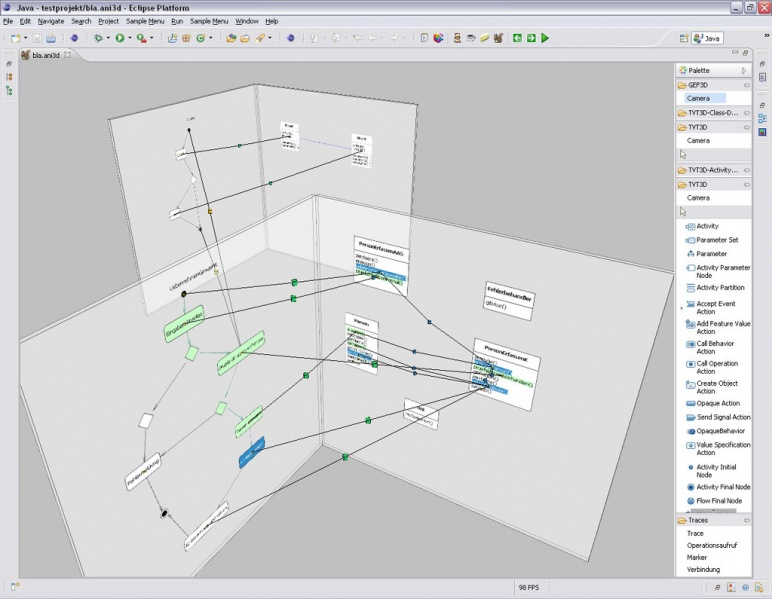
\includegraphics[height=10cm]{772px-ScreenshotTVT3D.jpg}
\caption{Kombination mehrerer 2D-Editoren in einer 3D-Ansicht von \cite{www:gef3d}}\label{related:gef3d-twt3d}\end{figure}
\begin{figure}[htbp]
\centering
\capstart

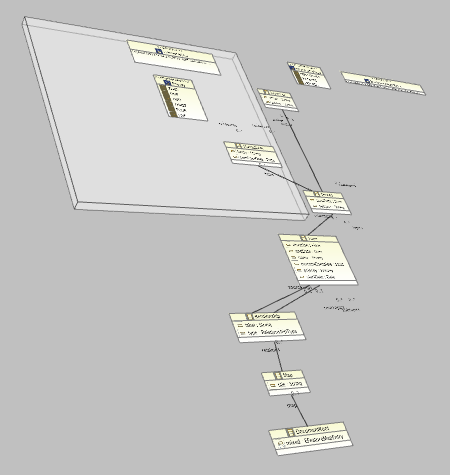
\includegraphics[height=10cm]{gef3d-ecore-rev436.png}
\caption{3D-Ecore-Editor von \cite{www:gef3ddevblog}}\label{related:gef3d-ecore}\end{figure}
\pagebreak

\section{3D-Prozessvisualisierung}
\label{related:d-prozessvisualisierung}
Arbeiten, die sich speziell mit 3D-Visualisierungen im Kontext des Prozessmanagements (Prozessmodellierung, -simulation) beschäftigen, werden hier vorgestellt.
Außerdem wird gezeigt, wie sich abstrakte Modelle in eine virtuelle Umgebung integrieren lassen.


\subsection{3D-Repräsentation von Prozessmodellen}
\label{related:betz}\label{related:d-reprasentation-von-prozessmodellen}
Von \cite{betz_3d_2008} wird die Visualisierung von Prozessen mittels dreidimensional dargestellter Petrinetze vorgestellt.
Es werden verschiedene Szenarien gezeigt, in denen 3D-Visualisierungen gewinnbringend genutzt werden könnten.

Es wird das Problem angesprochen, dass für die Modellierung von Prozessen oft verschiedene Diagrammtypen nötig seien, zwischen denen in üblichen 2D-Werkzeugen zeitraubend gewechselt werden müsse.
Mehrere Diagrammtypen in eine 3D-Ansicht zu integrieren könne hier Abhilfe schaffen.

Als Beispiel wird \hyperref[related:betz-org-process]{Abbildung  \ref*{related:betz-org-process}} eine Kombination eines Organisationsmodells mit einem Prozessmodell gezeigt.
Neben den Beziehungen zwischen Aktivitäten im Prozessmodell und den Rollen des Organisationsmodells sei es gleichzeitig möglich, Beziehungen im Organisationsmodell, wie die Generalisierung von Rollen oder die Zuordnung von Aktoren zu Rollen zu visualisieren.
\begin{figure}[htbp]
\centering
\capstart

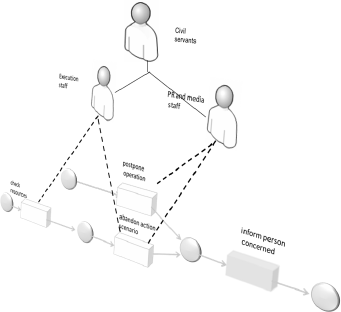
\includegraphics[height=10cm]{betz_org_process.png}
\caption{Darstellung von Beziehungen zwischen Prozess- und Organisationsmodell aus \cite{betz_3d_2008}}\label{related:betz-org-process}\end{figure}

Ein weiteres Anwendungsszenario für 3D-Visualisierungen sei es, Ähnlichkeiten zwischen verschiedenen Prozessmodellen aufzuzeigen.

Im 3D-Raum sei es einfach möglich, zu vergleichende Prozesse nebeneinander auf parallelen Ebenen im Raum zu platzieren.
Verbindungen zwischen Modellelementen der gegenüber gestellten Prozessmodelle könnten dafür genutzt werden, mit verschiedenen Metriken berechnete Ähnlichkeitswerte anzuzeigen.
Wie in \hyperref[related:betz-vergleich-pm]{Abbildung  \ref*{related:betz-vergleich-pm}} zu sehen ist werden die Werte sowohl durch die Beschriftung als auch durch die Dicke der Verbindungslinien visualisiert.
\begin{figure}[htbp]
\centering
\capstart

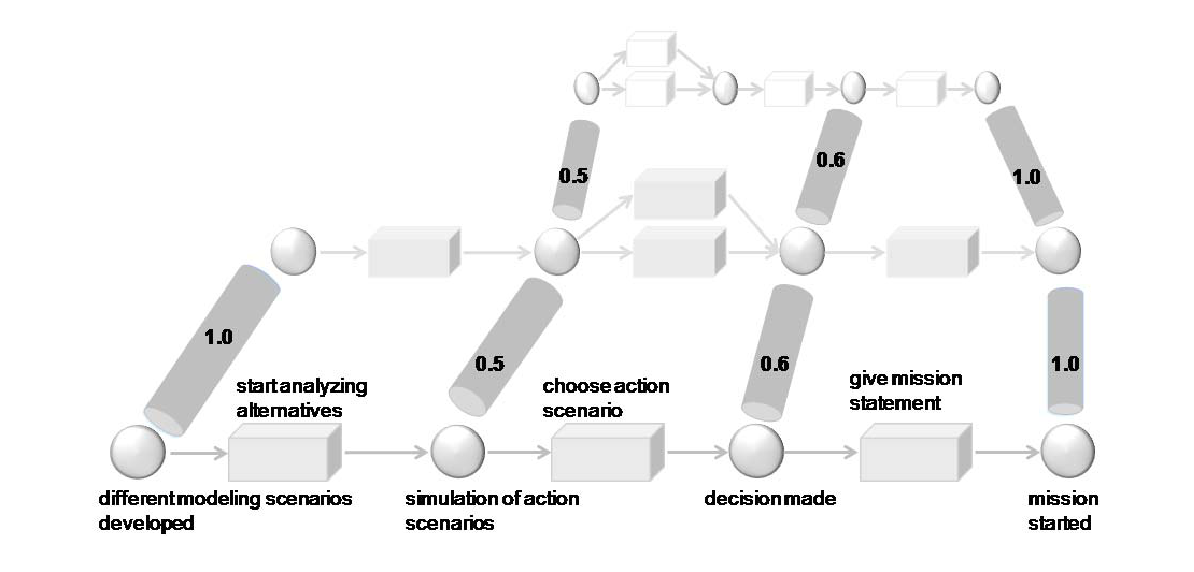
\includegraphics[height=8cm]{betz_vergleich_pm.png}
\caption{Visualisierung von Ähnlichkeiten zwischen Prozessmodellen aus \cite{betz_3d_2008}}\label{related:betz-vergleich-pm}\end{figure}

Außerdem könnten hierarchische Prozessdiagramme gut im dreidimensionalen Raum dargestellt werden.
Der Benutzer könne mehrere Verfeinerungsstufen des Modells in einer Ansicht sehen, wie in \hyperref[related:betz-prozess-verfeinerung]{Abbildung  \ref*{related:betz-prozess-verfeinerung}} gezeigt wird.
\begin{figure}[htbp]
\centering
\capstart

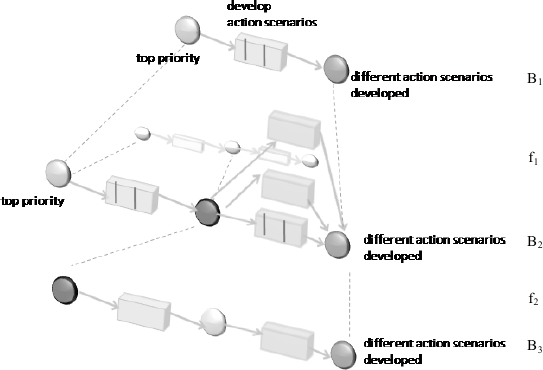
\includegraphics[height=8cm]{betz_prozess_verfeinerung.png}
\caption{Vier Verfeinerungsstufen eines Prozessmodells aus \cite{betz_3d_2008}}\label{related:betz-prozess-verfeinerung}\end{figure}


\subsection{3D-Visualisierung für die Prozesssimulation}
\label{related:d-visualisierung-fur-die-prozesssimulation}\label{related:schoenhage}
In \cite{schonhage_3d_2000} wird ein Prototyp einer interaktiven 3D-Umgebung vorgestellt, der dafür genutzt werden könne, Simulationen von Prozessen zu kontrollieren und dabei anfallende Daten zu visualisieren.
Der Prozess selbst wird, wie in \hyperref[related:schoenhage-graph]{Abbildung  \ref*{related:schoenhage-graph}} gezeigt, als 3D-Graph dargestellt, wobei Subgraphen durch den Benutzer nach Bedarf auf- und zugeklappt werden könnten.
Datenflüsse würden durch animierte Kugeln angezeigt, die sich entlang der Kanten von einem Aktivitätsknoten zum nächsten bewegen würden.
Der Anwender könne durch die Auswahl von Knoten und dem Drücken einer "`drill-down-Schaltfläche"' eine Visualisierung zugehöriger Prozessdaten öffnen – hier im Beispiel 3D-Histogramme – wie in \hyperref[related:schoenhage-all]{Abbildung  \ref*{related:schoenhage-all}} zu sehen ist. Im Beispiel zeigen die 3D-Histogramme eine Häufigkeitsverteilung (horizontal) von "`Wartezeiten"' im Laufe von vier Wochen.
Es sei möglich, Ansichten auf den Prozessgraphen zu speichern, um später wieder schnell zu diesen zurückspringen zu können.
\begin{figure}[htbp]
\centering
\capstart

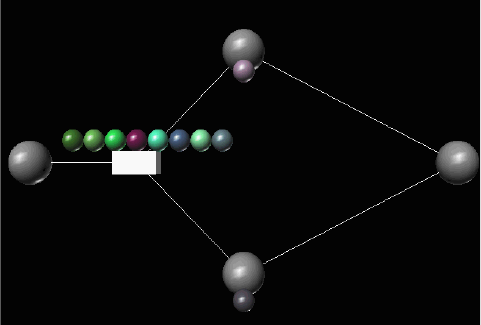
\includegraphics[height=9cm]{schoenhage_process.png}
\caption{Prozessgraph mit "`Datenflusskugeln"' aus \cite{schonhage_3d_2000}}\label{related:schoenhage-graph}\end{figure}
\begin{figure}[htbp]
\centering
\capstart

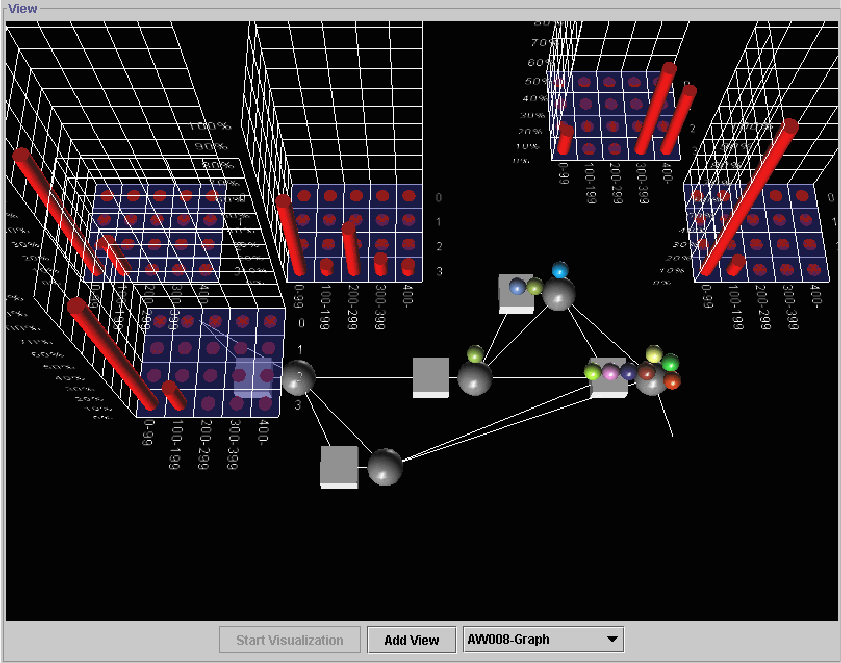
\includegraphics[height=12cm]{schoenhage_all.png}
\caption{Darstellung eines Prozesses mit assoziierten Daten (3D-Histogramme) aus \cite{schonhage_3d_2000}}\label{related:schoenhage-all}\end{figure}


\subsection{Modellierung von Prozessen in interaktiven, virtuellen 3D-Umgebungen}
\label{related:ross-brown}\label{related:modellierung-von-prozessen-in-interaktiven-virtuellen-3d-umgebungen}
In \cite{brown_conceptual_2010} wird ein Prototyp eines BPMN-Editors vorgestellt, der Prozesse innerhalb eine virtuellen 3D-Umgebung darstellt
Besonderer Wert sei auf die Zusammenarbeit zwischen mehreren Modellierern und die Prozesskommunikation – auch unter Beteiligung von Personen, die keine Modellierungsexperten sind – gelegt worden.
"`Naive stakeholders"' hätten oft Probleme, die abstrakte Welt der konzeptuellen Modellierung zu verstehen, weil der Bezug zu realen Gegenständen fehle.
Unter Zuhilfennahme einer "`virtuellen Welt"' (virtual reality), in welche abstrakte Prozessmodelle eingebettet sind, solle dies abgemildert werden.

In dieser Umgebung könnten Abbilder von realen Entitäten, die mit dem Prozess in Beziehung stehen oder mit diesem interagieren – beispielsweise verwendete Betriebsmittel oder ausführende Personen – dargestellt werden.
Dies könne auch dazu dienen, den Ort und die räumliche Anordnung von Prozessschritten, beispielsweise durch die Einbettung in ein virtuelles Gebäude, zu visualisieren.
Möglich sei auch eine Simulation der Prozessausführung in der virtuellen Welt.
Dadurch solle es den Beteiligten leichter möglich sein, festzustellen, ob das Modell die Realität richtig abbilde und ob eventuell Probleme bei der Umsetzung des Prozesses in der Realität auftreten könnten.

Wie in \hyperref[related:brown-process]{Abbildung  \ref*{related:brown-process}} zu sehen ist, werden Prozesse als 3D-Graph dargestellt, wobei als Knoten auf 3D-Objekte übertragene BPMN-Modellelemente genutzt werden.
Auf den Knoten können Informationen durch Texte oder statische Grafiken vermittelt werden.
\begin{figure}[htbp]
\centering
\capstart

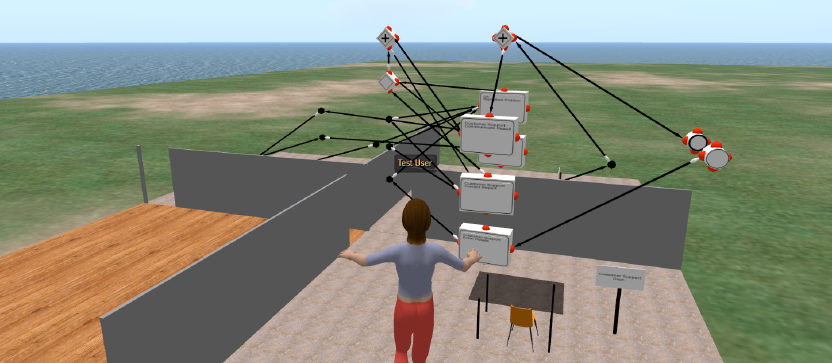
\includegraphics{brown_prozessgraph.png}
\caption{BPMN-Prozessgraph in virtueller Welt aus \cite{brown_conceptual_2010}}\label{related:brown-process}\end{figure}

Informationen auf den Objekten scheinen nur auf einer Seite dargestellt zu sein. Das ist problematisch, falls Modellelemente gedreht und Bewegungen um den Prozessgraphen herum ausgeführt werden.
Je nach Perspektive wäre es möglich, dass die Texte bzw. die Symbole nicht mehr sichtbar sind.
\hyperref[related:brown-process]{Abbildung  \ref*{related:brown-process}} zeigt auch, dass die gegenseitige Verdeckung von Modellelementen ebenfalls zu Schwierigkeiten bei der Lesbarkeit der Informationen führt.
Die Benutzer selbst werden, wie in \hyperref[related:brown-nodes]{Abbildung  \ref*{related:brown-nodes}} zu sehen ist, als Avatar gezeigt, welcher die Interaktion der Benutzer mit dem Modell für andere Teilnehmer zeigen soll.
\begin{figure}[htbp]
\centering
\capstart

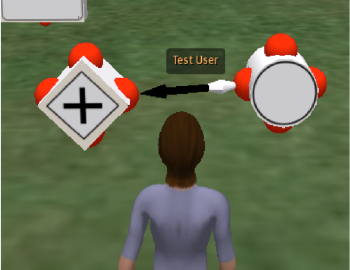
\includegraphics[height=6cm]{brown_nodes.png}
\caption{Benutzer-Avatar vor 3D-BPMN-Elementen aus \cite{brown_conceptual_2010}}\label{related:brown-nodes}\end{figure}

Es gebe die Möglichkeit, "`Kommentarwände"' zur Anzeige von Texten für die Kommunikation zwischen den Beteiligten aufzustellen.
Daneben könnten auch andere Multimedia-Inhalte wie Videos, Tonaufnahmen oder Statistiken zur Prozessausführung (über Web-Services) eingebettet werden.
Dies ist in \hyperref[related:brown-datadisplay]{Abbildung  \ref*{related:brown-datadisplay}} zu sehen.
\begin{figure}[htbp]
\centering
\capstart

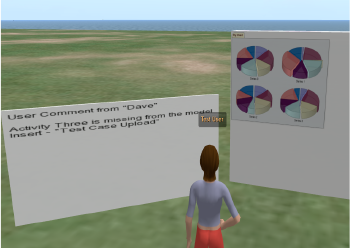
\includegraphics[height=6cm]{brown_datadisplay.png}
\caption{Kommentarwände und Multimedia-Inhalte in der virtuellen Welt aus \cite{brown_conceptual_2010}}\label{related:brown-datadisplay}\end{figure}


\section{Verbesserung der dreidimensionalen Darstellung von Graphen}
\label{related:verbesserung-der-dreidimensionalen-darstellung-von-graphen}
3D-Szenen werden auf üblichen Arbeitsplatz-Bildschirmen zu einer zweidimensionalen Projektion reduziert \cite{akenine-moller_real-time_2008}.
Dies bedeutet, dass die Vorteile einer dreidimensionalen Darstellung, welche sich aus der Tiefenwirkung ergeben, nicht vollständig zur Geltung kommen.
Um dies zu umgehen lassen sich Techniken wie die Stereoskopie, Bewegungsparallaxe\footnote{
Näheres zu Wahrnehmung von Tiefe siehe \cite{wickens_three_1989}, \cite{wp:bewegungsparallaxe} oder \cite{wp:stereoskopie}.
} oder voll immersive virtuelle Umgebungen (oft als CAVE bezeichnet\footnote{
Näheres zu CAVE-Systemen siehe \cite{cruz-neira_surround-screen_1993} oder \cite{wpe:cave}.
}) einsetzen.


\subsection{Nutzung von 3D-Effekten für einen verbesserten Tiefeneindruck}
\label{related:nutzung-von-3d-effekten-fur-einen-verbesserten-tiefeneindruck}\label{related:ware-graphs}
In \cite{ware_visualizing_2008} wird an Probanden untersucht, wie groß die Vorteile einer stereoskopischen 3D-Darstellung von umfangreichen Graphen im Vergleich zu einer 2D-Darstellung sind.
Als Maß für die "`Lesbarkeit"' wird hier das Abschneiden bei der Aufgabe, die Pfadlänge zwischen zwei markierten Knoten zu erkennen, genutzt.

Stereoskopische 3D-Darstellung sei besonders hilfreich, um dem Betrachter einen realistischen Tiefeneindruck zu vermitteln und damit das Erkennen von Verbindungen zu erleichtern.
Eine weitere Maßnahme, um den Tiefeneindruck zu verbessern, sei es, den Graphen ständig zu rotieren und damit die Bewegungsparallaxe zu nutzen\footnotemark[2].
Es zeigte sich, dass die Probanden – bei gleicher Fehlerrate – Verbindungen in 3D-Graphen erkennen hätten können, welche um eine Größenordung größer gewesen seien als die entsprechenden 2D-Graphen.

Dabei sei eine Anzeige mit einer sehr hohen Auflösung verwendet worden, die nahe an das Auflösungsvermögen des menschlichen Sehsystems herankomme.
Eine frühere Untersuchung mit ähnlicher Konzeption \cite{ware_evaluating_1996} zeigte deutlich kleinere Vorteile für die stereoskopische 3D-Darstellung.
Dies wird in der späteren Arbeit auf den Umstand zurückgeführt, dass hierbei Anzeigen mit einer viel niedrigeren Auflösung verwendet worden seien.


\subsection{3D-Visualisierung von Graphen in voll immersiven virtuellen Umgebungen}
\label{related:d-visualisierung-von-graphen-in-voll-immersiven-virtuellen-umgebungen}\label{related:halpin-social-net}
Neben der Anzeige von 3D-Graphvisualisierungen auf handelsüblichen Arbeitsplatz-Rechnern könnten dafür auch immersive 3D-Umgebungen (fully immersive virtual reality) genutzt werden.

So zeigt \cite{halpin_exploring_2008} die Visualisierung von sozialen Netzwerken in einer CAVE-Umgebung.
Benutzer könnten so direkt mit der Graphdarstellung der Daten in einer natürlichen Art und Weise interagieren und einen realitätsnahen räumlichen Eindruck von der virtuellen Welt bekommen.

Der Graph würde zu Beginn in einer "`2D-Darstellung"' in einer Ebene vor dem Benutzer angezeigt, wie in der \hyperref[related:halpin-extrude]{Abbildung  \ref*{related:halpin-extrude}} (unten) zu sehen ist.
Links ist zu sehen, wie durch das "`Berühren"' mit einem virtuellen Werkzeug (grauer Quader) die mit dem Knoten assoziierten Daten angezeigt werden können.

Wenn sich ein Benutzer speziell für die Verbindungen eines bestimmten Knoten interessiere, sei es möglich aus dieser Darstellung den gewünschten Knoten zu "`extrudieren"', also zu sich heranzuziehen.
Wie in \hyperref[related:halpin-extrude]{Abbildung  \ref*{related:halpin-extrude}} (rechts) zu sehen ist werden dadurch die Verbindungen des Knotens hervorgehoben.
\begin{figure}[htbp]
\centering
\capstart

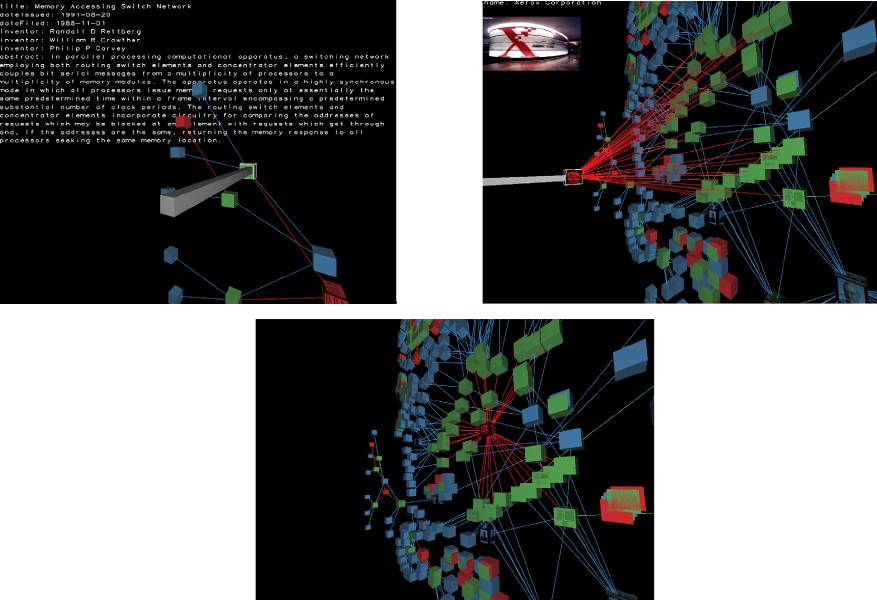
\includegraphics[height=11cm]{halpin_extrude_mod.png}
\caption{Visualisierung von semantischen Netzwerken aus \cite{halpin_exploring_2008}}\label{related:halpin-extrude}\end{figure}


\section{Zusammenfassung und Bewertung}
\label{related:zusammenfassung-und-bewertung}\label{related:related-zusammenfassung}
Es wurden verschiedene Ansätze gezeigt, zu einer 3D-Visualisierung von Informationen zu gelangen und deren Vorteile zu nutzen.
So lässt sich häufig der Ansatz beobachten, von einer bekannten 2D-Visualisierung auszugehen und diese in den 3D-Raum zu übertragen.
Dies war besonders bei den verschiedenen Arbeiten zu sehen, die sich mit 3D-UML beschäftigen.

Der vorliegende Abschnitt fasst die wichtigsten Nutzungmöglichkeiten der dritten Dimension zusammen, die in den gezeigten Arbeiten vorgeschlagen wurden.
Außerdem wird versucht, eine Einschätzung zu geben, wie vorteilhaft die gezeigte (3D-)Visualisierung im Vergleich zu einer reinen 2D-Darstellung ist.
Die folgende Tabelle gibt einen Überblick über die vorgestellten Verwendungsmöglichkeiten und deren möglichen Nutzen.

\begin{DUlineblock}{0em}
\item[] 
\end{DUlineblock}
\begin{tabular}{|c|c|c|c|c|}
\hline
Name & Ansatz & Domäne & 3. Dimension verwendet für & Nutzen\tabularnewline
\hline
\hline
McIntosh & 2,5D & UML(Zustand) & Visualisierung von Modellhierarchien & o\tabularnewline
\hline
Gil & 2,5D & UML(Sequenz) & Zeitachse, unterschiedl. Beziehungstypen & +\tabularnewline
\hline
Gogalla & 3D & UML(Klassen) & ``Wichtigkeit'' von Knoten & +\tabularnewline
\hline
Schönhage & 3D & Prozesssimulation & Darstellung von Ausführungsdaten & o\tabularnewline
\hline
Betz & 3D & Prozesse(Petrinetz) & mehrere Modelle/-typen, hierarchische Modelle & +\tabularnewline
\hline
Brown & 3D & Prozesse(BPMN) & Einbettung in virtuelle Umgebung & ++\tabularnewline
\hline
\end{tabular}
\begin{DUlineblock}{0em}
\item[] 
\end{DUlineblock}


\subsection{2,5D / 3D-Visualisierungen von Modellen}
\label{related:d-3d-visualisierungen-von-modellen}
Eine naheliegende Möglichkeit ist es, schon bekannte 2D-Modellierungssprachen wieder zweidimensional auf Flächen im 3D-Raum zu platzieren.
Dies wurde von {\hyperref[related:mcintosh]{\emph{McIntosh}}} (\autoref*{related:mcintosh}) für UML-Zustandsdiagramme, von {\hyperref[related:gil]{\emph{Gil und Kent}}} (\autoref*{related:gil}) oder bei {\hyperref[related:gef3d]{\emph{GEF3D}}} (\autoref*{related:gef3d}) gezeigt.
In der Tabelle werden solche Darstellungsformen als 2,5D-Ansatz bezeichnet.
Für die Implementierung bedeutet das, dass sich schon vorhandene 2D-Bibliotheken nutzen lassen, deren Grafikausgabe direkt auf die Flächen gezeichnet wird.
Für den Benutzer hat die Darstellung den Vorteil, dass sich die Darstellung der Modellelemente selbst nicht ändert und sich mehrere Modelle gleichzeitig darstellen lassen, indem die Ebenen zueinander versetzt werden.

Wie von {\hyperref[related:gil]{\emph{Gil und Kent}}} (\autoref*{related:gil}) erwähnt, lassen sich durch eine dreidimensionale Anordnung verschiedene Beziehungstypen besser unterscheiden als in reinen 2D-Ansichten.
Modellhierarchien und Beziehungen zwischen verschiedenen Modellen lassen sich gut darstellen, indem beispielsweise Linien zwischen assoziierten Elementen oder zu Unterdiagrammen gezeichnet werden.
Diese Beziehungen lassen sich schon durch die Anordnung optisch leicht von denjenigen unterscheiden, die innerhalb eines (Teil-)Modells bestehen und in einer Ebene mit den Modellelementen liegen.
In reinen 2D-Darstellungen ist diese Unterscheidung deutlich schwieriger und es muss üblicherweise auf unterschiedliche Farben oder Konnektoren zurückgegriffen werden.
Vor allem bei einer großen Anzahl von Elementen kann dies leicht zu verwirrenden Darstellungen führen.

Problematisch ist dagegen bei 2,5D-Ansätzen, dass es bei "`schrägen"' Betrachtungswinkeln schwierig wird, Informationen abzulesen, was sich besonders bei Schriftdarstellung bemerkbar machen wird.
Außerdem ist bei den bisher genannten Visualisierungsformen die Möglichkeit eingeschränkt, die dritte Dimension zur Vermittlung von zusätzlichen Informationen zu nutzen, da Elemente immer auf festen Ebenen platziert werden müssen.
Kontinuierliche Attribute der Modellelemente lassen sich so nicht darstellen.

Als Weiterentwicklung lässt sich die von {\hyperref[related:krolovitsch]{\emph{Krolovitsch und Nilsson}}} (\autoref*{related:krolovitsch}) vorgestellte Visualisierung von Zustandsdiagrammen betrachten, die ebenfalls 2D-Flächen nutzt, jedoch die Elemente aus der Ebene herausragen lässt.
So wirkt die Darstellung etwas "`plastischer"' und Strukturen lassen sich besser erkennen.
Die Höhe der Elemente lässt sich hier nutzen, um Werte von kontinuierlichen Modellattributen direkt zu visualisieren.

Interessant ist die dort gezeigte Möglichkeit, Subdiagramme temporär auszublenden und durch ein einzelnes Symbol zu ersetzen.
Dies wäre auch in der Prozessmodellierung hilfreich für die Darstellung von kompositen Prozessen.
So kann beispielsweise durch einen Doppelklick auf einen Prozessknoten ein weiteres Modell in der 3D-Szene angezeigt werden ohne ein neues Fenster zu öffnen, wie es in 2D-Werkzeugen praktiziert wird.

{\hyperref[related:betz]{\emph{Betz et al.}}} (\autoref*{related:betz}) zeigten für den Bereich der Prozessmodellierung die schon für die Softwaremodellierung genannten Nutzungsmöglichkeiten des 3D-Raums, also die hierarchische Darstellung von Prozessdiagrammen und die Visualisierung von Beziehungen zwischen unterschiedlichen Modellarten.

Von {\hyperref[related:gogolla]{\emph{Gogolla et al.}}} (\autoref*{related:gogolla}) wurden UML-Diagramme mit "`echten"', frei plazierbaren 3D-Objekten gezeigt.
Die dritte Dimension ("`Tiefe"') lässt sich dazu nutzen, schon durch Verbindungen festgelegte Zusammenhänge zu verdeutlichen oder um Attribute der Modellelemente zu visualisieren.

3D-Objekte wie Quader haben den Vorteil, dass sich Information – oft in Textform — auf mehreren Seiten darstellen lässt.
Wie von {\hyperref[related:dywer]{\emph{Dwyer}}} (\autoref*{related:dywer}) vorgeschlagen, gibt es die Möglichkeit, diese Objekte so zu drehen, dass dem Benutzer immer eine Seite zugewandt und damit gut lesbar ist.
Damit lassen sich solche Modelle besser aus unterschiedlichen Perspektiven betrachten als die vorgenannten 2,5D-Darstellungen.
Der Wechsel der Perspektive kann hilfreich sein, um unterschiedliche Aspekte der 3D-Szene gezielt betrachten zu können.
Beispielsweise können so Beziehungen zwischen Elementen auf parallelen Ebenen herausgestellt werden, indem die Szene "`von der Seite"' betrachtet wird.


\subsection{Integration von weiteren Informationen in 3D-Visualisierungen}
\label{related:informations-integration}\label{related:integration-von-weiteren-informationen-in-3d-visualisierungen}
Neben dem abstrakten Prozessmodell an sich lassen sich auch weitere Informationen dreidimensional darstellen.
So zeigten {\hyperref[related:schoenhage]{\emph{Schönhage et. al.}}} (\autoref*{related:schoenhage}), wie sich aus einer Simulation des Prozesses gewonnene Daten neben dem Prozessmodell anzeigen lassen.
Dies ist aber prinzipiell mit reinen 2D-Darstellungen ebenfalls möglich.
Um hier einen klaren Vorteil der 3D-Visualisierung erkennen zu können, müssen sich die Daten selbst sinnvoll dreidimensional darstellen lassen.
Ein Beispiel dafür sind die 3D-Histogramme, wie sie von Schönhage gezeigt wurden.

{\hyperref[related:ross-brown]{\emph{Brown}}} (\autoref*{related:ross-brown}) bettet die abstrahierte Darstellung des Prozesses in eine virtuelle Umgebung ein, welche den tatsächlichen Ausführungsort eines Prozesses räumlich abbilden kann.
Dies lässt sich als deutlicher Vorteil für die Nutzung von 3D-Visualisierungen im Vergleich zu 2D-Darstellungen festhalten.

Beispielsweise lassen sich Laufwege von am Prozess beteiligten Personen oder andere Vorgänge wie der Transport von Werkstücken (animiert) darstellen, um mögliche Probleme bei der Ausführung und Optimierungsmöglichkeiten aufzuzeigen.
So kann festgestellt werden, ob sich gewisse Wege verkürzen oder vermeiden lassen, indem Reihenfolge oder der Ausführungsort von Prozessschritten verändert werden.
Durch die Integration von Abbildern realer Objekte in die virtuelle Welt können abstrakte Konzepte des Prozessmodells veranschaulicht oder um weitere Informationen ergänzt werden.
Sinnvoll ist dies beispielsweise, um Veränderungen an einem Werkstück im Laufe eines Produktionsprozesses zu visualisieren, indem die Zwischenstufen dreidimensional neben den Prozessschritten abgebildet werden.

Eine andere denkbare Anwendung wäre eine Visualisierung der Platzverhältnisse in einer Ausführungsumgebung.
Wenn die Umgebung sowie sich darin befindliche Objekte relativ zueinander im richtigen Größenverhältnis und in der tatsächlichen Form dargestellt sind, könnte schon bei einer Betrachtung des Prozesses in der virtuellen Welt bemerkt werden, dass vorgesehene Ablageplätze in einem Lager oder Transportbehälter für ein Werkstück zu klein dimensioniert sind.

\hyperref[related:brown-airport]{Abbildung  \ref*{related:brown-airport}}\footnote{
Quelle: www.youtube.com/watch?v=aUBmvykDhB0. Das Video ist auch auf der beigelegten {\hyperref[anhang_b:anhang-dvd]{\emph{Systemanforderungen und Inhalt der DVD}}} (\autoref*{anhang_b:anhang-dvd}) zu finden.
} zeigt einen BPMN-Prozess in einer 3D-Umgebung, die mit Hilfe des von Brown vorgestellten Editors erstellt wurde und einen Flughafen darstellen soll.
Dies ließe sich prinzipiell auch mit einer 2D-Darstellung realisieren, indem die Szene von oben gezeigt wird.
Dadurch wird aber die Übersichtlichkeit eingeschränkt; die Möglichkeit, den Prozessgraphen im dreidimensionalen Raum in einer Ebene über dem Boden zu zeigen, erweist sich hier als Vorteil.
Ebenso bietet es sich an, im 3D-Raum die Betrachtungsperspektive nach Bedarf zu verändern.
Ist die Blickrichtung des Betrachters annähernd parallel zum Untergrund wie in der Abbildung, lassen sich auch weit entfernte "`Stationen"' des Prozesses erkennen.
Ein Blick von oben auf die Szene aus größerer Entfernung gibt dagegen einen groben Überblick über die gesamte Prozessstruktur.
\begin{figure}[htbp]
\centering
\capstart

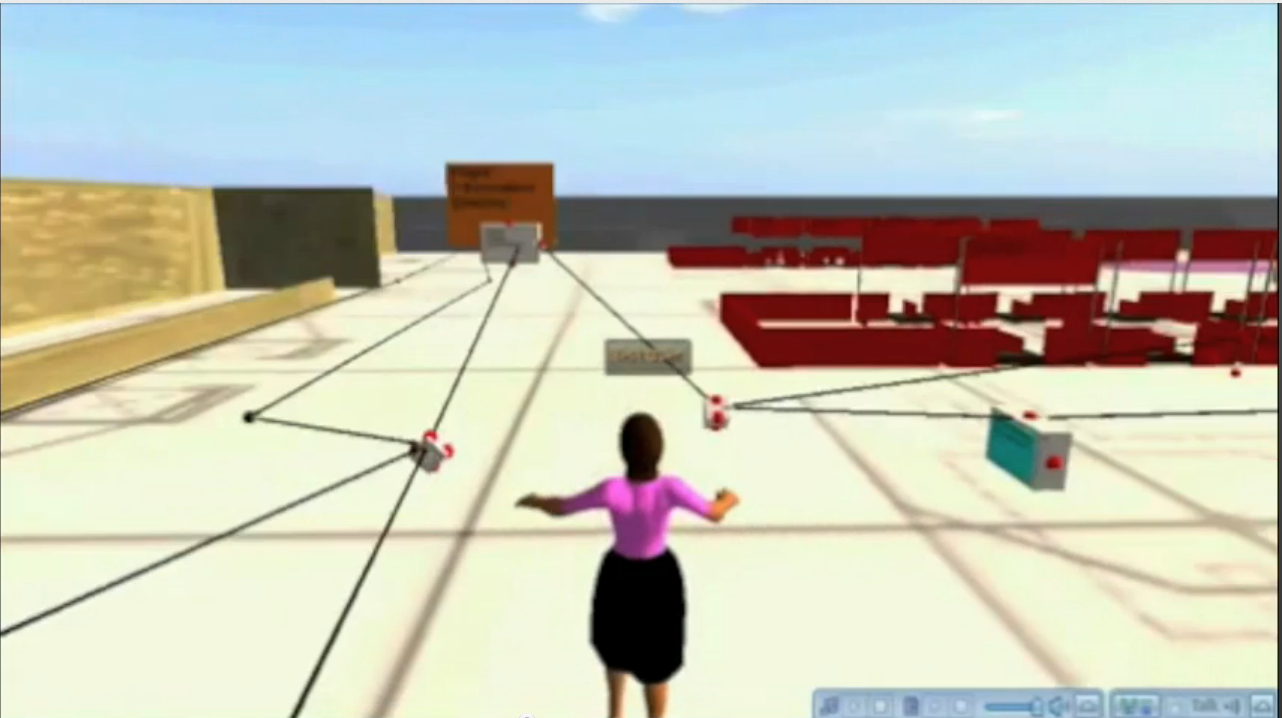
\includegraphics[width=16.5cm]{brown_airport.png}
\caption{Visualisierung eines BPMN-Prozesses in einer virtuellen Umgebung}\label{related:brown-airport}\end{figure}


\subsection{Effizienz und Akzeptanz von 3D-Darstellungen?}
\label{related:effizienz-und-akzeptanz-von-3d-darstellungen}
Die wichtige Frage, ob und in welchen Situationen 3D-Visualisierungen Vorteile gegenüber 2D-Darstellungen haben, die über eine reine Verbesserung des Erscheinungsbilds hinausgehen,  kann von den gezeigten Arbeiten sicher nicht vollständig beantwortet werden.
Es wurden immerhin einige Hinweise zur Effizienz gegeben, indem beispielsweise Benutzerstudien durchgeführt wurden, welche Vorteile für 3D-Darstellungen in der Softwaremodellierung andeuten, jedoch auch Probleme aufzeigen \cite{dwyer_three_2001} \cite{mcintosh_x3d-uml:_2008} \cite{halpin_exploring_2008}.
Untersuchungen zur Effizienz, die sich speziell auf die Prozessmodellierung beziehen, ließen sich nicht finden.

Inwieweit 3D-Darstellungen für die Prozessmodellierung nützlich sind, hängt sicher auch davon ab, wie komplex die Modelle sind.
Einfache Modelle lassen sich auch mit den Hilfsmitteln der 2D-Visualisierung adäquat darstellen.
Prinzipiell ist eine 2D-Darstellung von Modellen wohl für die meisten Benutzer etwas intuitiver zu verstehen, da diese schon länger verbreitet und beispielsweise aus UML- oder BPMN-Werkzeugen bekannt ist.
Wie erwähnt, werden die Vorteile von 3D-Darstellungen dann deutlich, wenn es darum geht, viele Verbindungstypen darzustellen oder hierarchische Modelle in einer Szene darzustellen.
Ob 3D-Visualisierungen effizient sind und ob sich deren höhere Komplexität – sowohl für den Benutzer als auch für die Implementierung – auszahlt muss daher sicher abhängig vom konkreten Anwendungsfall bewertet werden.

Bei der Betrachtung der Effizienz muss auch berücksichtigt werden, dass die Erfahrung der Benutzer mit 3D-Darstellungen aus anderen Bereichen – beispielsweise aus Computerspielen oder 3D-CAD-Werkzeugen – eine Rolle spielt
\cite{dwyer_three_2001} \cite{ware_visualizing_2008} \cite{schonhage_3d_2000}.
Es stellt sich die Frage, wie unerfahrene Benutzer an 3D-Werkzeuge für die Prozessmodellierung herangeführt werden könnten, um diese effizient nutzen zu können.

In eine ähnliche Richtung geht die Fragestellung, inwieweit 3D-Werkzeuge überhaupt von Benutzern akzeptiert werden.
\cite{schonhage_3d_2000} bemerkte, dass 3D-Visualisierungen oft als reines "`Spielzeug"' angesehen würden, die keinen wirklichen Nutzen gegenüber 2D-Darstellungen brächten, sondern bestenfalls nur "`schöner"' aussähen.
Daher ist es wichtig, 3D-Visualisierungen für den Benutzer möglichst hilfreich und intuitiv zu gestalten, so dass deren Vorteile klar erkennbar sind.
Um eine hohe Akzeptanz zu erreichen müssten aber auch technische Probleme wie die schlechte Verfügbarkeit von 3D-tauglichen Eingabegeräten oder zu langsame Hardware\footnote{
Die besagte Arbeit ist 2000 entstanden. Sicherlich ist die Geschwindigkeit heutzutage ein kleineres Problem, aber es lässt sich nicht vernachlässigen. Gerade bei aufwändigen Grafikeffekten oder der Verarbeitung von komplexen Eingabedaten kann man leicht an die Grenzen der Rechenleistung stoßen.
} gelöst werden.
So ergeben sich große Herausforderungen, sowohl auf der konzeptuellen Ebene als auch auf der Seite der Implementierung von 3D-Visualisierungen und -Modellierungswerkzeugen.


\subsection{Verwendbare Vorarbeiten und Schlussfolgerungen für die Arbeit}
\label{related:verwendbare-vorarbeiten-und-schlussfolgerungen-fur-die-arbeit}
In den vorgestellten Arbeiten wurden einige Prototypen für 3D-Modellierungswerkzeuge entwickelt.
Allerdings war nur von \cite{dwyer_three_2001} eine freie Version im Internet auffindbar.
Diese ist allerdings technisch auf einem ziemlich alten Stand und lässt in Sachen Bedienung eher zu wünschen übrig.

Frei verfügbare Softwareprojekte, die schon ein flexibles 3D-Prozessmodellierungswerkzeug realisieren ließen sich nicht finden.
Als Grundlage für ein solches Werkzeug könnte möglicherweise GEF3D dienen, was jedoch nicht weiter verfolgt wurde.
Negativ könnte bei GEF3D gesehen werden, dass in letzter Zeit relativ wenige Änderungen an der Codebasis erfolgten und insgesamt eher wenig Aktivität festzustellen ist.

Ein Blick in den Quellcode zeigte, dass das Projekt noch auf "`alter"' OpenGL-Funktionalität aufbaut und damit die Möglichkeiten moderne Grafikhardware nicht nutzt.
Bei der vorliegenden Arbeit stand es aber im Vordergrund, eine möglichst flexible und "`zukunftsorientierte"' Grundlage für ein (anpassbares) Prozessmodellierungswerkzeug zu legen, wozu auch eine Grafikausgabe auf dem aktuellen Stand der Technik gehört.

Aus den hier vorgestellten Arbeiten ließen sich jedoch einige Konzepte ableiten, die in i\textgreater{}PM 3D realisiert wurden.
Es ist für die Arbeit sinnvoll, einen möglichst allgemeinen Visualisierungsansatz zu wählen, der es erlaubt, verschiedene Nutzungsmöglichkeiten der dritten Dimension umzusetzen und diese für verschiedene Anwendungsfälle im Prototypen zu evaluieren.
Daher soll der Prototyp grundsätzlich eine 3D-Graphvisualisierung von Prozessen unterstützen, wie es beispielsweise von {\hyperref[related:ross-brown]{\emph{Brown}}} (\autoref*{related:ross-brown}) gezeigt wurde. ({\hyperref[einleitung:anforderungen]{\emph{Anforderung (a)}}} (\autoref*{einleitung:anforderungen})).
Die Knoten des Graphen werden selbst dreidimensional dargestellt und sind frei in der 3D-Szene platzierbar. Dies stellt prinzipiell den flexibelsten Ansatz dar.
Eine 2,5D oder gar 2D-Darstellung lässt sich als Sonderfall einer 3D-Darstellung betrachten.
So kann die Darstellung oder die Platzierbarkeit von Elementen – ausgehend vom gewählten 3D-Ansatz – wieder eingeschränkt werden, falls sich dies für eine Anwendung als vorteilhaft herausstellen sollte.

Abstrakte Prozessmodelle in eine virtuelle Welt einzubetten und so räumliche Information zu nutzen stellt einen vielversprechenden Ansatz dar, aus dreidimensionalen Darstellungen einen großen Vorteil zu ziehen.
Dadurch wird {\hyperref[einleitung:anforderungen]{\emph{Anforderung (b)}}} (\autoref*{einleitung:anforderungen}) motiviert, beliebige 3D-Objekte in die Szene einfügen zu können, um damit abstrakte Modellelemente zu illustrieren oder virtuelle Ausführungsumgebungen visualisieren zu können.


\chapter{Verwendete Techniken und Software}
\label{verwendet::doc}\label{verwendet:verwendete-techniken-und-software}

\section{Scala}
\label{verwendet:scala}
Die Implementierung des i\textgreater{}PM3D-Projekts erfolgte zum größten Teil in der Programmiersprache Scala \cite{odersky_programming_2011} \cite{www:scala}.
Die Verwendung von Scala ergab sich aus der Entscheidung, die in Scala implementierte Simulations-Middleware {\hyperref[verwendet:simulatorx]{\emph{Simulator X}}} (\autoref*{verwendet:simulatorx}) als Basis für den Prototypen zu verwenden.

Scala wird als "`objektfunktionale"' Programmiersprache charakterisiert.
"`Objektfunktional"' soll die Bestrebungen ausdrücken, Aspekte aus funktionalen und objektorientierten Programmiersprachen zu einer flexiblen und effektiven Programmiersprache zu kombinieren.

Scala wird zur Zeit vorwiegend auf der Java VM genutzt, wobei der Compiler auch in der Lage ist, CIL-Code für die .NET-Runtime zu erzeugen.
i\textgreater{}PM3D läuft wegen einiger Abhängigkeiten von Java-Bibliotheken bisher ausschließlich auf der Java VM.

Die "`objektorientierte Facette"' Scalas orientiert sich an den Konzepten von Java, bietet aber einige Erweiterungen.
Hier werden nur Features kurz vorgestellt, die für die Implementierung besonders hilfreich waren und in späteren Kapiteln erwähnt werden.


\subsection{Traits}
\label{verwendet:traits}\label{verwendet:id1}
Als Erweiterung zu Java unterstützt Scala eine (eingeschränkte) Mehrfachvererbung von Implementierungscode über sog. \emph{Traits}.
Traits kann man sich als ein Java-Interface vorstellen, in dem Methoden schon vorimplementiert sein können.
Zur Vereinfachung dürfen Traits keinen Konstruktor definieren.

Neben der Verwendung als "`Interface"' – wie in Java – werden diese oft genutzt, um wiederverwendbare Code-Einheiten zu realisieren, die sich in verschiedenen Klassen einsetzen lassen.
Traits werden daher oft als \textbf{Mixin} bezeichnet.
Wie ein Trait zu einer Klasse hinzugefügt wird – auch \textbf{einmischen} genannt – zeigt das folgende Scala-Codebeispiel:

\begin{Verbatim}[commandchars=\\\{\}]
\PYG{k}{class} \PYG{n+nc}{Example} \PYG{k}{extends} \PYG{n+nc}{BaseClass} \PYG{k}{with} \PYG{n+nc}{MixinTrait}
\end{Verbatim}

\code{Example} wird hiermit von \code{BaseClass} abgeleitet und \code{MixinTrait} eingemischt.

In dieser Arbeit werden Traits in UML-Diagrammen als Klasse mit dem Stereotyp \emph{\textless{}\textless{}trait\textgreater{}\textgreater{}} dargestellt und Assoziationen zu einmischenden Klassen mit \emph{\textless{}\textless{}mixin\textgreater{}\textgreater{}} versehen.


\subsection{Objects}
\label{verwendet:objects}
Anstelle der aus Java bekannten statischen Klassenmethoden oder Singleton-Klassen wird in Scala das \emph{object}-Konstrukt genutzt.
\emph{Objects} können Klassen "`erweitern"', das bedeutet, dass das \emph{Object} als Instanz der Klasse betrachtet werden kann.
Als Beispiel sei hier ein ausführbares Scala-Programm gezeigt, welches eine (im Sinne von Java statische) Methode definiert und aufruft:

\begin{Verbatim}[commandchars=\\\{\}]
\PYG{k}{object} \PYG{n+nc}{Main} \PYG{k}{extends} \PYG{n+nc}{App} \PYG{o}{\PYGZob{}}
    \PYG{k}{def} \PYG{n}{hello}\PYG{o}{(}\PYG{o}{)} \PYG{o}{\PYGZob{}}
        \PYG{n}{println}\PYG{o}{(}\PYG{l+s}{"Hello World"}\PYG{o}{)}
    \PYG{o}{\PYGZcb{}}
    \PYG{n}{hello}\PYG{o}{(}\PYG{o}{)}
\PYG{o}{\PYGZcb{}}
\end{Verbatim}


\subsection{Actors}
\label{verwendet:id2}\label{verwendet:actors}
Ein sinnvoller Einsatzbereich von Scala ist unter anderem die Erstellung von parallelen und verteilten Anwendungen.
Dazu kommt oft das \textbf{Actor-Modell} \cite{haller_scala_2009} zum Einsatz, das früher schon in der Programmiersprache Erlang \cite{www:erlang} realisiert wurde.

Grundlage für das Actor-Modell ist das \textbf{message passing}, welches eine asynchrone Kommunikation zwischen den beteiligten Actors ermöglicht.
Berechnungen innerhalb einzelner Actors können so prinzipiell parallel erfolgen.
Informationen werden ausschließlich über Nachrichten ausgetauscht. Es ist nicht erlaubt, auf gemeinsame, veränderliche Datenstrukturen zuzugreifen.
Actors können auf unterschiedlichen (Java-)Threads ausgeführt werden und somit auch mehrere Prozessorkerne nutzen, ohne den Programmierer mit der manuellen Verwaltung und Synchronisation von Threads zu belasten.

In Scala wird eine Nachricht oft durch ein Objekt einer \textbf{case class} dargestellt\footnote{
Das \emph{case class}-Konstrukt erzeugt eine Klasse, in der gewisse Methoden vorimplementiert sind, die bspw. einen inhaltlichen Vergleich mit dem ==-Operator oder einen Einsatz im \emph{pattern matching} erlauben. Siehe \cite{odersky_programming_2011}.
}.
Diese Klassen werden dafür genutzt, Daten zu unveränderlichen Objekten zusammenzufassen, wie im folgenden Code gezeigt wird:

\begin{Verbatim}[commandchars=\\\{\}]
\PYG{k}{case} \PYG{k}{class} \PYG{n+nc}{Message}\PYG{o}{(}\PYG{n}{data}\PYG{k}{:} \PYG{k+kt}{String}\PYG{o}{,} \PYG{n}{number}\PYG{k}{:} \PYG{k+kt}{Int}\PYG{o}{)}
\PYG{n}{receivingActor} \PYG{o}{!} \PYG{n+nc}{Message}\PYG{o}{(}\PYG{l+s}{"hello!"}\PYG{o}{,} \PYG{l+m+mi}{42}\PYG{o}{)}
\end{Verbatim}

In der zweiten Zeile wird ein Objekt der Klasse \code{Message} erzeugt und an \code{receivingActor} gesendet.


\subsection{Implizite Methoden}
\label{verwendet:implicit}\label{verwendet:implizite-methoden}
Es ist möglich, sog. "`implizite Methoden"' zu definieren, welche vom Compiler automatisch eingesetzt werden können, wenn diese benötigt werden\footnote{
Welche Bedingungen dafür erfüllt sein müssen, kann bspw. in \cite{odersky_programming_2011} nachgelesen werden.
}.
Besonders praktisch sind diese Methoden für die Realisierung von "`transparenten"' Adaptern, wie sie im vorliegenden Projekt genutzt werden.
Diese werden auch \textbf{implizite Wrapper} genannt.

\begin{Verbatim}[commandchars=\\\{\}]
\PYG{k}{implicit} \PYG{k}{def} \PYG{n}{conceptToAdapter}\PYG{o}{(}\PYG{n}{m}\PYG{k}{:} \PYG{k+kt}{MConcept}\PYG{o}{)} \PYG{k}{=} \PYG{k}{new} \PYG{n+nc}{MConceptAdapter}\PYG{o}{(}\PYG{n}{m}\PYG{o}{)}
\end{Verbatim}

Mit dieser Definition lassen sich nun Methoden, die für \code{MConceptAdapter} definiert sind auch auf Objekten des Typs \code{MConcept} aufrufen als wären sie Teil von \code{MConcept}.


\subsection{Parser-Kombinatoren}
\label{verwendet:parser-kombinatoren}\label{verwendet:id5}
Die Scala-Standardbibliothek bietet eine einfache Möglichkeit, Parser mit Hilfe von Parser-Kombinatoren \cite{odersky_programming_2011} zu erstellen.
Dies wird in dieser Arbeit für die Laden von Modellen in einer textuellen Repräsentation eingesetzt.

Einfache Parser werden von Parser-Kombinatoren zu komplexeren Parsing-Ausdrücken zusammengesetzt.
Parser sind als Funktionen definiert, die einen String auf eine beliebige Ausgabe abbilden.
Parser-Kombinatoren sind Funktionen höherer Ordnung, die Parser als Eingabe erwarten und als Ausgabe wiederum eine Parser-Funktion liefern.

In Scala werden die Bestandteile der textuellen Eingabe oft in Objekte von \emph{case classes} übersetzt, die zusammen einen Syntaxbaum der Eingabe ergeben.

Folgende Parser-Funktion

\begin{Verbatim}[commandchars=\\\{\}]
\PYG{k}{def} \PYG{n}{stringAssignment} \PYG{k}{=} \PYG{n}{ident} \PYG{o}{\PYGZti{}} \PYG{o}{(}\PYG{l+s}{"="} \PYG{o}{\PYGZti{}\textgreater{}} \PYG{n}{stringLits} \PYG{o}{\textless{}\PYGZti{}} \PYG{l+s}{";"}\PYG{o}{)} \PYG{o}{\PYGZca{}\PYGZca{}} \PYG{o}{\PYGZob{}}
  \PYG{k}{case} \PYG{n}{id} \PYG{o}{\PYGZti{}} \PYG{n}{stringLits} \PYG{k}{=\textgreater{}} \PYG{n+nc}{LiteralTypeAssignment}\PYG{o}{(}\PYG{n}{id}\PYG{o}{,} \PYG{n}{stringLits}\PYG{o}{)}
\PYG{o}{\PYGZcb{}}
\end{Verbatim}

würde beispielsweise die {\hyperref[grundlagen:lmm]{\emph{LML-String-Zuweisung}}} (\autoref*{grundlagen:lmm})

\begin{Verbatim}[commandchars=\\\{\}]
\PYG{n}{functions} \PYG{o}{=} \PYG{l+s}{"a"}\PYG{o}{,} \PYG{l+s}{"test"}\PYG{o}{;}
\end{Verbatim}

erkennen und in ein Scala-Objekt des Typs \code{LiteralTypeAssignment} übersetzen. Dieser Typ könnte wie folgt definiert sein:

\begin{Verbatim}[commandchars=\\\{\}]
\PYG{k}{case} \PYG{k}{class} \PYG{n+nc}{LiteralTypeAssignment}\PYG{o}{(}\PYG{n}{id}\PYG{k}{:} \PYG{k+kt}{String}\PYG{o}{,} \PYG{n}{stringLiterals}\PYG{k}{:} \PYG{k+kt}{List}\PYG{o}{[}\PYG{k+kt}{String}\PYG{o}{]}\PYG{o}{)}
\end{Verbatim}


\section{Simulator X}
\label{verwendet:simulatorx}\label{verwendet:simulator-x}
\emph{Simulator X} \cite{latoschik_simulator_2011} \cite{fischbach_sixtons_2011} ist ein Prototyp einer neuartigen Simulationsplattform, welche die Realisierung von interaktiven Echtzeit-Anwendungen besonders einfach machen soll. Der Fokus liegt dabei auf Anwendungen aus der Computergrafik, besonders in Verbindung mit multimodalen Bedienschnittstellen, welche neuartige Eingabemethoden wie Gesten- und Sprachsteuerung nutzen.

Simulator X setzt auf dem {\hyperref[verwendet:actors]{\emph{(Scala-)Actor-Modell}}} (\autoref*{verwendet:actors}) auf und bietet daher dessen Eigenschaften wie die Ausnutzung mehrerer Prozessorkerne und eine asynchrone Kommunikation zwischen Actors.
Sog. \textbf{Komponenten} (\code{Component}) sind die grundlegenden Bestandteile einer Simulator X-Anwendung. Komponenten sind als Actor realisiert und stellen eine wohldefinierte Funktionalität für das System zur Verfügung.

Von Simulator X wird eine Reihe von Komponenten bereitgestellt, beispielsweise die für i\textgreater{}PM3D verwendete Gestenerkennung und eine \emph{Physikkomponente} für physikalische Simulationen (bspw. für Gravitation und Erkennung von Kollisionen zwischen Simulationsobjekten).
Andere, typischerweise für Simulator X-Anwendungen verwendete Komponenten umfassen Renderkomponenten für die Realisierung der Grafikausgabe oder Komponenten zur Beeinflussung der Simulationsobjekte durch künstliche Intelligenz.

Simulator X bietet – ebenfalls auf Basis des Actor-Modells – ein Event-System und eine Abstraktion globaler Zustandsvariablen an.
Komponenten können sich beim Event-System für bestimmte Ereignisse, die von anderen Komponenten ausgelöst werden, registrieren und so automatisch benachrichtigt werden.

Globale Zustandsvariablen, \textbf{SVars} genannt, vereinfachen für den Programmierer den Umgang mit verteilten Daten.
Ein bestimmtes Datum wird von genau einem Actor, dem "`Besitzer"' verwaltet.
Andere Actors besitzen nur eine spezielle Referenz auf den Wert und müssen mit dem Besitzer kommunizieren, um den Wert auszulesen oder zu manipulieren.
Diese Kommunikation wird von Simulator X automatisch und transparent für den Programmierer durchgeführt.
\hyperref[verwendet:svars]{Abbildung  \ref*{verwendet:svars}} zeigt ein Beispiel, in welchem \code{actor\#1} der Besitzer der SVar ist und die beiden anderen Actors nur Referenzen auf diese SVar halten.
\begin{figure}[htbp]
\centering
\capstart

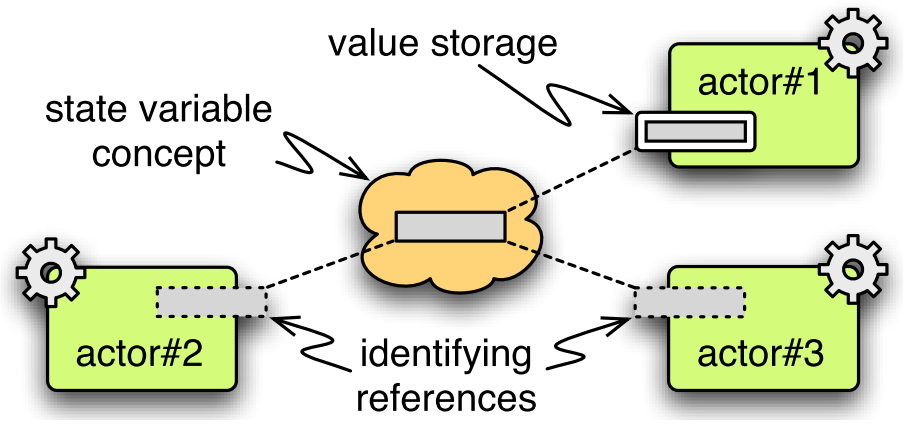
\includegraphics[height=5cm]{simxactorvars.png}
\caption{Zustandsvariablen-Konzept aus \cite{latoschik_simulator_2011}}\label{verwendet:svars}\end{figure}

Eine zugeordnete \code{SVarDescription}benennt die SVar, gibt ihr einen Scala-Datentyp und definiert deren Semantik in einer Anwendung.
So lässt sich beispielsweise definieren, dass der Wert einer SVar eine Farbe darstellt, welche durch eine Klasse \code{Vec4} repräsentiert wird.

Eine Menge von SVars ergibt zusammen eine \textbf{Entität}, die genau ein Simulationsobjekt repräsentiert\footnote{
Dies könnte im Prozesseditor beispielsweise ein Modellelement wie ein Prozess oder eine Kontrollflusskante sein.
}.
So kann durch die Manipulation der \code{Color}-SVar einer bestimmten Entität deren Farbe festgelegt werden.

\code{Entities} werden durch den Programmierer mittels einer \code{EntityDescription} beschrieben, die aus mehreren \code{Aspect}-Definitionen aufgebaut sein kann \cite{wiebusch_enhanced_2012}.
\textbf{Aspects} beschreiben eine wohldefinierte Facette der Entität und sind einer bestimmten Komponente zugeordnet.
So gibt es beispielsweise Grafik- oder Physik-\code{Aspects}.

Ein \code{Aspect} legt fest, wie eine Komponente mit einem bestimmten Simulationsobjekt umgehen soll.
Über die \code{Aspect}-Definition können Werte durch den Benutzer vorgegeben werden, die das Verhalten der Komponente im Bezug auf die zugehörige Entität festlegen.
So lässt sich beispielsweise über einen Physik-\code{Aspect} festlegen, welche physikalische Repräsentation für die Entität genutzt werden soll, beispielsweise ein Quader mit bestimmten Abmessungen und einer Masse.
Für eine Renderkomponente kann der Pfad zu einer 3D-Objektdatei angegeben werden, welche als grafische Repräsentation für die Simulationsobjekt auf dem Bildschirm angezeigt werden soll.

Simulator X befindet sich gerade in der Entwicklung. Für das vorliegende Projekt wird eine Version von August 2011 genutzt.


\section{OpenGL / LWJGL}
\label{verwendet:opengl-lwjgl}\label{verwendet:opengl}
Um die Grafikausgabe von i\textgreater{}PM3D zu realisieren, wird die plattformunabhängige 3D-Schnittstelle OpenGL \cite{opengl} genutzt.

Zur Anbindung an OpenGL wird die Java-Bibliothek LWJGL (Lightweight Java Gaming Library) \cite{www:lwjgl} in der Version 2.8.2 eingesetzt.
Zusätzlich stellt LWJGL eine Schnittstelle für den Zugriff auf Tastatur- und Mausdaten zur Verfügung.

Hier sollen nur einige wenige Hinweise zu "`modernem"' OpenGL (ab Version 3.0) und den in späteren Kapiteln benutzten Begriffen gegeben werden.
Näheres kann in \cite{wright_opengl_2010} oder unter \cite{opengl} nachgelesen werden.
Allgemeines zu Begriffen aus der 3D-Computergrafik findet sich bei \cite{akenine-moller_real-time_2008}.

In älteren OpenGL-Versionen (1.x) wurden von OpenGL viele, fest eingebaute Funktionen wie die Berechnung der Beleuchtung und Texturierung bereitgestellt, die nur aktiviert und konfiguriert werden mussten.
Deshalb wird "`altes"' OpenGL oft mit dem Begriff \emph{fixed-function-Pipeline} \cite{akenine-moller_real-time_2008} in Verbindung gebracht.

Mit Version 3.0 wurden viele dieser Funktionen aus dem Kern von OpenGL entfernt. In neueren Versionen müssen die Berechnungen durch den Programmierer selbst in \emph{Shadern} implementiert werden.
Das neue Konzept gibt jedoch dem Programmierer die Freiheit, auch völlig neue Grafikeffekte zu implementieren, die mit der \emph{fixed-function-Pipeline} nicht oder nur schwer umsetzbar gewesen wären.
Diese Möglichkeit wurde in der vorliegenden Arbeit für einige "`Spezialeffekte"' genutzt, die sich auf diesem Weg einfach realisieren ließen.

Bei \textbf{Shadern} handelt es sich um kleine Programme, die in der Programmiersprache GLSL (OpenGL Shading Language) geschrieben und die direkt auf dem Grafikprozessor von sog. \emph{Shader-Einheiten} ausgeführt werden.
Code kann in GLSL in Funktionen ausgelagert und so in mehreren Shadern genutzt werden.
Shader erfüllen verschiedene Aufgaben an von OpenGL festgelegten Positionen innerhalb der Render-Pipeline \cite{www:glpipe} \cite{akenine-moller_real-time_2008}.

In OpenGL 4 werden folgende Typen unterstützt:
\begin{description}
\item[{Vertex-Shader}] \leavevmode
arbeiten auf einzelnen Vertices eines 3D-Objekts \footnote{
Ein Vertex ist ein "`Eckpunkt"' eines 3D-Objekts, welches in OpenGL üblicherweise als ein aus Dreiecken aufgebautes Gitter beschrieben wird.
} und sind beispielsweise für die Transformation von 3D-Modellkoordinaten in das von OpenGL benutzte Koordinatensystem zuständig.

\item[{Geometry-Shader}] \leavevmode
können aus den gegebenen Vertices neue Zwischen-Vertices erzeugen.

\item[{Fragment-Shader}] \leavevmode
werden einmal pro Fragment aufgerufen\footnote{
Ein Fragment entspricht – vereinfacht gesagt – einem Pixel auf dem Bildschirm.
} und implementieren beispielsweise Texturierung und Beleuchtung.

\item[{Tesselation-Shader (ab OpenGL 4)}] \leavevmode
können komplett neue Geometrien erzeugen.

\end{description}

Mit \textbf{Vertex-Attributen} lassen sich beliebige Daten pro Vertex an die Shaderprogramme übertragen; häufig sind das Vertexkoordinaten\footnote{
Vertexkoordinaten sind die Koordinaten des Punkts im 3D-Raum. OpenGL "`rendert"' ein 3D-Objekt, indem eine Liste von Vertices der Reihe nach gezeichnet wird.
}, Normalen\footnote{
Normalen werden vor allem für die Berechnung der Beleuchtung benötigt.
} und Texturkoordinaten\footnote{
Texturkoordinaten sind häufig zweidimensional und werden vor allem dazu genutzt, 2D-Grafiken auf 3D-Objekten zu positionieren.
}.
Vertex-Attribute werden vom Shader aus Puffern im Grafikspeicher ausgelesen, welche als Vertex Buffer Objects (VBO) bezeichnet werden.

\textbf{Uniforms} übermitteln Werte an Shaderprogramme, die üblicherweise für ein ganzes Grafikobjekt gelten. Dies können beispielsweise Lichtparameter oder Farbwerte sein.


\section{Sonstiges}
\label{verwendet:sonstiges}

\subsection{StringTemplate}
\label{verwendet:id12}\label{verwendet:stringtemplate}
Um Prozessmodelle in einer textuellen Form speichern zu können, wird die Template-Bibliothek \emph{StringTemplate} (ST) in der Version 4.0.4 verwendet. \cite{parr_language_2009}
ST folgt dem Prinzip, einen Text mit "`Platzhaltern"' (Attributen) zu definieren. Die Attribute werden aus dem Anwendungsprogramm heraus gesetzt und so das Template mit Inhalt gefüllt.
Diese Schicht sorgt unter anderem dafür, dass beliebige Scala-Objekte als Java-Bean an ST weitergegeben werden können, auch wenn sie selbst nicht der Java-Bean-Konvention entsprechen.
In folgendem Beispiel wird ein Template erstellt, welches die LMM-Zuweisung \code{function = "test"} produziert:

\begin{Verbatim}[commandchars=\\\{\}]
\PYG{k}{val} \PYG{n}{assignTemplate} \PYG{k}{=} \PYG{l+s}{"\textless{}attribName\textgreater{} = \PYGZbs{}"\textless{}value\textgreater{}\PYGZbs{}""}
\PYG{k}{val} \PYG{n}{assignST} \PYG{k}{=} \PYG{n+nc}{ST}\PYG{o}{(}\PYG{n}{assignTemplate}\PYG{o}{)}
\PYG{n}{assignST}\PYG{o}{.}\PYG{n}{addAll}\PYG{o}{(}
    \PYG{l+s}{"attribName"} \PYG{o}{-\textgreater{}} \PYG{l+s}{"function"}\PYG{o}{,}
    \PYG{l+s}{"value"} \PYG{o}{-\textgreater{}} \PYG{l+s}{"test"}\PYG{o}{)}
\PYG{k}{val} \PYG{n}{output} \PYG{k}{=} \PYG{n}{assignST}\PYG{o}{.}\PYG{n}{render}
\end{Verbatim}


\subsection{Simplex3D-Math}
\label{verwendet:simplex3d-math}\label{verwendet:simplex3d}
Im i\textgreater{}PM3D-Projekt wird die in Scala implementierte Mathematikbibliothek \emph{Simplex3D-Math} in der Version 1.3 \cite{www:simplex3d} genutzt.
Durch die Bibliothek werden Matrizen, Vektoren und dazugehörige Utility-Funktionen bereitgestellt. Deren API orientiert sich weitgehend an der OpenGL Shading Language.


\chapter{Einordnung in das Gesamtprojekt i\textgreater{}PM3D}
\label{ipm3d:ipm3d}\label{ipm3d:einordnung-in-das-gesamtprojekt-i-pm3d}\label{ipm3d::doc}
Diese Arbeit und die dazugehörige Implementierung sind im Rahmen des i\textgreater{}PM3D-Projekts entstanden. Das Ziel des Projekts ist es, einen Prototypen eines grafischen 3D-Prozessmodellierungswerkzeugs zu erstellen, der prinzipielle Vor-und Nachteile von 3D-Editoren zeigen und als Grundlage für weitere Arbeiten in dieser Richtung dienen soll.
Das vorliegende Kapitel gibt eine Übersicht über das i\textgreater{}PM3D-Projekt\footnote{
Dieses Kapitel ist in Zusammenarbeit mit \cite{buchi} und \cite{uli} entstanden und in jenen Arbeiten in ähnlicher Form zu finden.
}.


\section{Übersicht über die Projektbestandteile}
\label{ipm3d:ipm3d-uebersicht}\label{ipm3d:ubersicht-uber-die-projektbestandteile}
In der Übersichtsgrafik \hyperref[ipm3d:ipm3d-konzeptionelle-uebersicht]{Abbildung  \ref*{ipm3d:ipm3d-konzeptionelle-uebersicht}} wird der konzeptionelle Aufbau des Projektes veranschaulicht.
Bestandteile, mit denen sich die vorliegende Arbeit befasst, sind darin farbig hervorgehoben (rechts).
In das i\textgreater{}PM 3D-Projekt sind ebenfalls die Bachelorarbeiten von Sebastian Buchholz \cite{buchi} und Uli Holtmann \cite{uli} einzuordnen, die die übrigen Bestandteile von i\textgreater{}PM3D beschreiben.
\begin{figure}[htbp]
\centering
\capstart

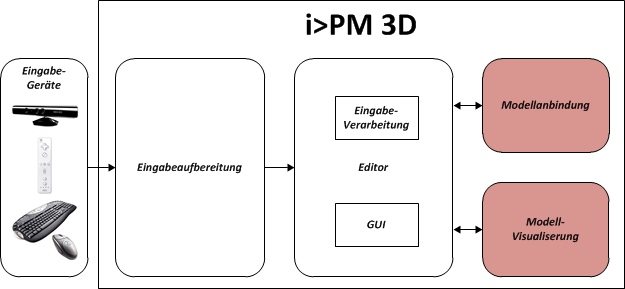
\includegraphics[width=15cm]{ipm3d-uebersicht.eps}
\caption{Übersicht über die Bestandteile von i\textgreater{}PM3D}\label{ipm3d:ipm3d-konzeptionelle-uebersicht}\end{figure}

Im Folgenden werden die einzelnen Projektbestandteile kurz vorgestellt und miteinander in Beziehung gesetzt.


\subsection{Visualisierung}
\label{ipm3d:ipm3d-visualisierung}\label{ipm3d:visualisierung}
Eine zentrale Fragestellung bei der Realisierung eines grafischen Prozessmodellierungswerkzeugs ist es, auf welche Weise Prozessmodelle visualisiert werden sollen.

Elemente aus dem Prozessmodell sollen in einer für den Benutzer leicht verständlichen Art und Weise angezeigt werden, die die Möglichkeiten des dreidimensionalen Raums nutzt.
Die Darstellung soll dabei an die aus 2D-Prozessmodellierungswerkzeugen bekannten grafischen Notationen angelehnt sein.
Prozessmodelle in i\textgreater{}PM3D werden in einer graphbasierten Form, also durch Knoten und damit verbundenen Kanten dargestellt.
Zusätzlich zu den eigentlichen Prozessmodellelementen gibt es die Möglichkeit, beliebige 3D-Objekte anzuzeigen. Dies kann beispielsweise dafür genutzt werden, um abstrakte Konzepte mit Abbildern von realen Objekten zu illustrieren.

Wie in der Computergrafik üblich wird das Prinzip einer virtuellen Kamera benutzt, durch die der Benutzer die Szene beobachtet ("`Egoperspektive"').
Durch Verschieben und Rotieren der Kamera kann sich der Benutzer in der virtuellen Umgebung "`bewegen"' und die dargestellten Prozessdiagramme aus verschiedenen Perspektiven betrachten.
Knoten und Szenenobjekte sind frei drehbar um alle drei Achsen und unter Beibehaltung der Seitenverhältnisse skalierbar. Sie können prinzipiell frei in der 3D-Szene platziert werden.
Die Visualisierung von Modellen in i\textgreater{}PM3D wird in der vorliegenden Arbeit näher {\hyperref[visualisierung:visualisierung]{\emph{vorgestellt}}} (\autoref*{visualisierung:visualisierung}).


\subsection{Modellanbindung}
\label{ipm3d:modellanbindung}
Ein Modellierungswerkzeug muss die Fähigkeit haben, bestehende Modelle aus einer physischen Repräsentation zu laden, das Modell beziehungsweise dessen Elemente zu bearbeiten und wieder zu speichern.
Außerdem sollen neue Modelle erstellt werden können.
In i\textgreater{}PM 3D kann die grafische Modellierungssprache (in einem gewissen Rahmen) ohne Änderungen am Programmcode modifiziert werden, da die abstrakten Modellelemente und deren (visuelle) Repräsentation jeweils durch ein zur Laufzeit geladenes Metamodell beschrieben werden.
Die in einem Prozessmodell verwendeten abstrakten Modellelemente (bspw. ein "`Prozessknoten"') sowie deren aktuelle Repräsentation im Modelleditor (bspw. das "`Aussehen"' und die Position eines Prozessknotens) werden in separaten Modellen abgelegt.
In der \hyperref[ipm3d:ipm3d-konzeptionelle-uebersicht]{Abbildung  \ref*{ipm3d:ipm3d-konzeptionelle-uebersicht}} werden diese Modelle als "`Prozess-Modell"' bzw. als "`Editor-Modell"' bezeichnet.

Der grundsätzliche Aufbau und die Anpassbarkeit der Modell-Hierarchie wird in {\hyperref[modellhierarchie:modellhierarchie]{\emph{dieser Arbeit}}} (\autoref*{modellhierarchie:modellhierarchie}) besprochen.
Außerdem werden die verwendeten Metamodelle im Detail {\hyperref[metamodelle:metamodelle]{\emph{beschrieben}}} (\autoref*{metamodelle:metamodelle}) und ein Beispiel gezeigt, wie sich neue Modellelemente ergänzen lassen.

Es ist ebenfalls Gegenstand dieser Arbeit, die Einbindung der Modell-Funktionen in den Prototypen zu realisieren.
In der Übersichtsgrafik \hyperref[ipm3d:ipm3d-konzeptionelle-uebersicht]{Abbildung  \ref*{ipm3d:ipm3d-konzeptionelle-uebersicht}} wird dieser Teil des Projekts als {\hyperref[modellanbindung:modellanbindung]{\emph{"`Modellanbindung"'}}} (\autoref*{modellanbindung:modellanbindung}) bezeichnet.


\subsection{GUI}
\label{ipm3d:gui}\label{ipm3d:ipm3d-gui}
Dem Benutzer wird das 3D-Prozessdiagramm in einer interaktiven Umgebung präsentiert, die das Erstellen, Bearbeiten und Löschen von Elementen erlaubt.

Die verschiedenen Funktionen des Prozessmodellierungswerkzeugs wie das Erstellen von Modellelementen und das Laden von Modellen lassen sich durch grafische Menüs aktivieren, die über der 3D-Szene gezeichnet werden und die an das Bedienkonzept verbreiteter 2D-Anwendungen mit grafischer Oberfläche angelehnt sind.
Für das Erstellen von neuen Knoten und Szenenobjekten wird ein Menü – auch als "`Palette"' bezeichnet – bereitgestellt, über welches die zur Verfügung stehenden Objekte durch einen Klick auf eine Schaltfläche erzeugt werden können.
Attribute der Modellelemente, die entweder die Visualisierung selbst oder das damit verbundene Element des Prozessmodells betreffen, können in einem in einem Menü angezeigt und bearbeitet werden.
Die Menüs werden in der Übersichtsgrafik \hyperref[ipm3d:ipm3d-konzeptionelle-uebersicht]{Abbildung  \ref*{ipm3d:ipm3d-konzeptionelle-uebersicht}} als GUI zusammengefasst.


\subsection{Eingabeaufbereitung und Editor}
\label{ipm3d:eingabeaufbereitung-und-editor}
Eine wichtige Anforderung an den Prototypen ist, dass verschiedene Arten von Eingabegeräten unterstützt, neue Geräte einfach angebunden und – soweit sinnvoll – nebeneinander benutzt werden können.
Die von den Eingabegeräten gelieferten Daten unterscheiden sich je nach Art des Geräts und der verwendeten Schnittstelle deutlich voneinander.
Daher ist es sinnvoll, von den Eingabegeräten und deren Schnittstellen zu abstrahieren. Dies wird erreicht, indem die Eingabedaten aller Geräte von einer Eingabeschicht aufbereitet und an eine vereinheitlichte Schnittstelle zur Bedienung der Anwendung weitergeleitet werden. Diese Schnittstelle zur Eingabeverarbeitung wird, zusammen mit dem GUI, in der Übersichtsgrafik \hyperref[ipm3d:ipm3d-konzeptionelle-uebersicht]{Abbildung  \ref*{ipm3d:ipm3d-konzeptionelle-uebersicht}} als \emph{Editor} bezeichnet.

Mit der Realisierung des \emph{Editors} sowie mit der Aufbereitung der Daten, die von Tastatur und Maus geliefert werden befasst sich \cite{uli}.


\subsection{Neuartige Eingabegeräte}
\label{ipm3d:neuartige-eingabegerate}
Neben den für Arbeitsplatzrechner üblichen Eingabegeräten Tastatur und Maus, soll der Editor auch mittels "`neuartiger"' Eingabegeräte bedienbar sein, die sich besonders für die Interaktion mit virtuellen 3D-Umgebungen eignen könnten.
Dabei sind besonders solche Geräte interessant, die auch an einem handelsüblichen, aktuellen Desktop-PC angeschlossen werden können und relativ "`preiswert"' sind.
Die Bereitstellung von neuartigen Eingabegeräten und die Aufbereitung der Eingabedaten werden von der Arbeit \cite{buchi} abgedeckt, welche sich speziell mit der Anbindung der Microsoft Kinect und der Nintendo WiiMote befasst. Neben der direkten Nutzung dieser Geräte als "`Mausersatz"' \footnote{
Dies bedeutet in diesem Zusammenhang, dass die Geräte einen Cursor ("`Mauszeiger"') steuern, der die aktuelle Position in einer zweidimensionalen Ebene anzeigt. Bei einem "`Klick"' wird eine Aktion auf dem darunter befindlichen Objekt ausgelöst.
} werden auch mit den Geräten ausgeführte Gesten und ein spezielles Kinect-Menü als Eingabemethode untersucht und für das Projekt nutzbar gemacht.

Diese Beiträge sind in der Übersichtsgrafik \hyperref[ipm3d:ipm3d-konzeptionelle-uebersicht]{Abbildung  \ref*{ipm3d:ipm3d-konzeptionelle-uebersicht}} unter "`Eingabegeräte"' und "`Eingabeaufbereitung"' zu finden.


\section{i\textgreater{}PM3D als Simulator X - Applikation}
\label{ipm3d:i-pm3d-als-simulator-x-applikation}
i\textgreater{}PM3D ist als Anwendung auf Basis von {\hyperref[verwendet:simulatorx]{\emph{Simulator X}}} (\autoref*{verwendet:simulatorx}) konzipiert.
\hyperref[ipm3d:ipm3d-simulatorx]{Abbildung  \ref*{ipm3d:ipm3d-simulatorx}} zeigt, wie die Architektur des Projekts auf den von Simulator X bereitgestellten Funktionalitäten aufbaut.
In den beiden folgenden Abschnitten wird zusammengefasst, welche Änderungen am Simulator-X-Basissystem vorgenommen worden sind und wie die im letzten Abschnitt dargestellten Projektteile im Kontext von \emph{Simulator X} umgesetzt werden.
\begin{figure}[htbp]
\centering
\capstart

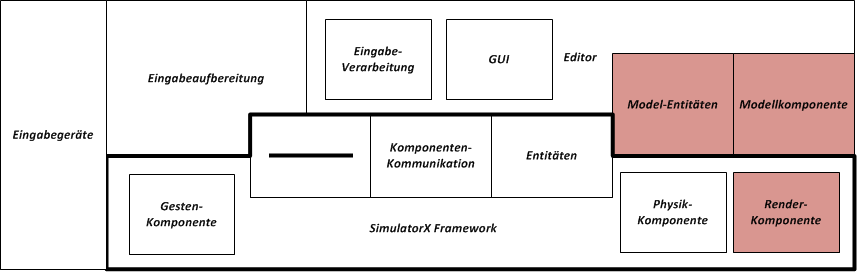
\includegraphics{ipm3d-simulatorx.png}
\caption{Architektur von i\textgreater{}PM3D, aufbauend auf Simulator X}\label{ipm3d:ipm3d-simulatorx}\end{figure}


\subsection{Modifikationen an Simulator X}
\label{ipm3d:mod-simx}\label{ipm3d:modifikationen-an-simulator-x}
Für i\textgreater{}PM3D wurde die von {\hyperref[verwendet:simulatorx]{\emph{Simulator X}}} (\autoref*{verwendet:simulatorx}) bereitgestellte Physik-Komponente für spezielle Aufgaben erweitert. Die Physikengine wird für die Selektion von Modellobjekten, für die Realisierung von "`Gravitationsebenen"', und die Erkennung von Kollisionen zwischen Modellobjekten eingesetzt. Den Einsatz Physikkomponente und die projektspezifischen Modifikationen beschreibt \cite{buchi}.

Die ebenfalls mitgelieferte Renderkomponente, die für die grafische Ausgabe auf Basis von OpenGL zuständig ist, war für das Projekt allerdings nicht sinnvoll nutzbar.
Daher wurde diese durch eine Anbindung an die im Rahmen dieser Arbeit entwickelte, flexible {\hyperref[renderbib:render-bibliothek]{\emph{Render-Bibliothek}}} (\autoref*{renderbib:render-bibliothek}) ersetzt, welche die einfache Erstellung von neuen Modell-Figuren ermöglicht und die Möglichkeiten moderner OpenGL-Grafikprogrammierung nutzt.
Die Anbindung an \emph{Simulator X} wird durch die in \hyperref[ipm3d:ipm3d-simulatorx]{Abbildung  \ref*{ipm3d:ipm3d-simulatorx}} gezeigte {\hyperref[renderkomponente:renderkomponente]{\emph{Renderkomponente}}} (\autoref*{renderkomponente:renderkomponente}) geleistet.


\subsection{Modellkomponente und Modell-Entitäten}
\label{ipm3d:modellkomponente-und-modell-entitaten}
Die im vorherigen Abschnitt als \emph{Modellanbindung} bezeichneten Funktionalitäten werden im Simulator X - Kontext durch die \textbf{Modellkomponente} realisiert, die dem Editor eine Schnittstelle zur Verfügung stellt über welche die genannten Aktionen ausgelöst werden können.
Die Modellelemente selbst zu bearbeiten, also deren Visualisierungsparameter und Prozessmodellattribute sowie die Position, Größe und Orientierung im Raum zu ändern, wird durch die von der Modellkomponente bereitgestellten \textbf{Modell-Entitäten} ermöglicht, welche durch den Editor manipuliert werden.

Dem Simulator X - Konzept folgend, beschreiben diese \emph{Entities} außerdem, wie die dazugehörigen Objekte von der Physikkomponente behandelt und wie sie von der Renderkomponente angezeigt werden.
Näheres zur Modellkomponente und den Modell-Entitäten ist im Kapitel zur {\hyperref[modellanbindung:modellanbindung]{\emph{Modellanbindung}}} (\autoref*{modellanbindung:modellanbindung}) zu finden.


\subsection{Editor-Komponente und Eingabekonnektoren}
\label{ipm3d:editor-komponente-und-eingabekonnektoren}
Die Bedienschnittstelle, in Abbildung 3.2 als Editor beschrieben, ist eine Simulator X Komponente.
Wird eine Modell-Entity fertiggestellt, wird sie dem Editor übergeben, so dass dieser sie in seine eigenen Datenstrukturen einbringen und für den Benutzer ansprechbar machen kann.
Die Konnektoren der Eingabeaufbereitungsschicht setzen auf keiner Simulator X Komponente auf, benutzen dafür aber das Simulator X Event-System um die aufbereiteten Eingabedaten an die Bedienschnittstelle zu senden.
Eine ausführlichere Beschreibung der Editor-Komponente, Eingabekonnektoren sowie der Kommunikation untereinander und mit anderen Komponenten ist bei \cite{uli} zu finden.


\chapter{Modellhierarchie}
\label{modellhierarchie:modellhierarchie}\label{modellhierarchie::doc}\label{modellhierarchie:id1}
In der Prozessmodellierung ist es sinnvoll, neben den Modellen auch die zugrundeliegende Modellierungssprache und Visualisierung an spezielle Anforderungen anpassen zu können (siehe {\hyperref[grundlagen:metamodellierung]{\emph{Metamodellierung}}} (\autoref*{grundlagen:metamodellierung})). Daher war eine solche Flexibilität auch für das vorliegende Arbeit erwünscht ({\hyperref[einleitung:anforderungen]{\emph{Anforderung (d)}}} (\autoref*{einleitung:anforderungen})).

Daher wurde das Konzept verfolgt, die verwendete grafische Modellierungssprache über austauschbare Metamodelle zu definieren. (\emph{Anforderung (c)})
Ein wichtiger Punkt ist, dass sich die abstrakte Syntax der Sprache und die konkrete Syntax (die "`Visualisierung"') getrennt beschreiben lassen.
Diesem Konzept folgt das bereits vorgestellte {\hyperref[grundlagen:mdf]{\emph{Model Designer Framework}}} (\autoref*{grundlagen:mdf}).
Die hier vorgestellte Modellhierarchie ist ähnlich zu der von MDF definierten aufgebaut und übernimmt einige Begriffe von dort.
Auf wichtige Unterschiede wird in diesem Kapitel explizit hingewiesen.

Das Konzept und die Implementierung der vorliegenden Arbeit erreicht jedoch nicht die Flexibilität von MDF, da hier ein Modellierungswerkzeug für die POPM und kein generisches Framework realisiert werden sollte.
Dennoch ist es möglich, in einem gewissen Rahmen Modifikationen an den verwendeten Modellelementen vorzunehmen und deren Visualisierung anzupassen.

Inwieweit sich die Modelle anpassen lassen und welche Einschränkungen bestehen wird im aktuellen Kapitel und bei der näheren Vorstellung der {\hyperref[metamodelle:metamodelle]{\emph{Metamodelle}}} (\autoref*{metamodelle:metamodelle}) deutlich.
Am Ende des nächsten Kapitels ist ein {\hyperref[metamodelle:beispiel-neues-element]{\emph{Anwendungsbeispiel}}} (\autoref*{metamodelle:beispiel-neues-element}) zu finden, welches zeigt, wie neue Elemente zur Modellierungssprache hinzugefügt werden können.

Die Anpassbarkeit der konkreten Syntax hat für den hier realisierten Prototypen vor allem den praktischen Nutzen, dass leicht mit der Visualisierung experimentiert werden kann, ohne den Quellcode der Anwendung ändern und neu übersetzen zu müssen.
Grundsätzlich lässt sich auch die verwendete Modellierungssprache komplett austauschen, jedoch wird in dieser Arbeit davon ausgegangen, dass das vorgegebene {\hyperref[metamodelle:pmm]{\emph{Prozess-Metamodell}}} (\autoref*{metamodelle:pmm}) genutzt wird.

\hyperref[modellhierarchie:modellhierarchie-diagram]{Abbildung  \ref*{modellhierarchie:modellhierarchie-diagram}} zeigt, wie sich die Hierarchie der Modelle darstellt, welche sich in einen \textbf{Editor-Model-Stack} und einen \textbf{Domain-Model-Stack} aufteilt.
Nach einer kurzen Vorstellung der Modellierungssprache wird eine Übersicht über die beiden Model-Stacks gegeben.
\begin{figure}[htbp]
\centering
\capstart

\includegraphics[width=16cm]{modellhierarchie.eps}
\caption{Modellhierarchie in i\textgreater{}PM3D (angelehnt an MDF \cite{roth_konzeption_2011})}\label{modellhierarchie:modellhierarchie-diagram}\end{figure}


\section{LMMLight}
\label{modellhierarchie:lmmlight}\label{modellhierarchie:id2}
Die Modelle werden mit Hilfe einer Metamodellierungssprache spezifiziert, die vom {\hyperref[grundlagen:lmm]{\emph{Linguistic Meta Model}}} (\autoref*{grundlagen:lmm}) abgeleitet ist.
Zum weiteren Verständnis ist es ausreichend, die in diesem Abschnitt gezeigten Grundelemente und Prinzipien zu kennen.

Die hier verwendete Sprache, im Folgenden \textbf{LMMLight} genannt, folgt in vielen Aspekten LMM, ohne jedoch alle weiterführenden Modellierungsmuster zu unterstützen, um eine einfache Implementierung zu ermöglichen.
Konkret hat dies zur Folge, dass der textuelle Modell-Editor von OMME für die Erstellung von LMMLight-Modellen sinnvoll genutzt werden kann, solange auf die nicht unterstützten Modellierungsmuster verzichtet wird.

LMMLight unterstützt das Muster der \textbf{Spezialisierung von Instanzen} (\code{concreteUseOf}), welches unter anderem für die Realisierung des {\hyperref[grundlagen:tvk]{\emph{Typ-Verwendungs-Konzepts}}} (\autoref*{grundlagen:tvk}) genutzt wird.
Im Gegensatz zu LMM lassen sich in Spezialisierungen alle Attributzuweisungen des spezialisierten Concepts ohne Einschränkung überschreiben.


\section{Editor-Model-Stack}
\label{modellhierarchie:id3}\label{modellhierarchie:editor-model-stack}
Der \emph{Editor-Model-Stack} von i\textgreater{}PM3D enthält alle Modelle, die dafür zuständig sind, die Visualisierungsparameter eines Domänenmodells zu beschreiben.
Außerdem werden hier Parameter spezifiziert oder gesetzt, welche die physikalische Repräsentation oder die für das Modellelement angebotenen Funktionalitäten im interaktiven Modellierungswerkzeug beeinflussen.
Näheres hierzu wird im nächsten Kapitel erläutert.
Mit "`Repräsentation"' ist im Folgenden die Gesamtheit dieser Parameter gemeint.

Die Verknüpfung mit dem \emph{Domain-Model-Stack} wird hergestellt, indem in Concepts des \emph{Editor-Model-Stacks} eine Referenz auf \emph{Domain-Model-Stack}-Concepts angegeben wird (\hyperref[modellhierarchie:editor-domain-conn]{Abbildung  \ref*{modellhierarchie:editor-domain-conn}}).
In \hyperref[modellhierarchie:modellhierarchie-diagram]{Abbildung  \ref*{modellhierarchie:modellhierarchie-diagram}} wird dies durch gestrichelte Pfeile dargestellt.
Besagte Referenzen werden durch das Attribut \code{modelElementFQN} angegeben, welchem der vollqualizierte Name (FQN) des referenzierten Concepts zugewiesen wird.
Vollqualifizierte Namen entstehen nach dem Schema \textless{}Model\textgreater{}.\textless{}Level\textgreater{}.\textless{}Package\textgreater{}.\textless{}Concept\textgreater{}, beispielsweise \code{EMM.D1.nodeFigures.ProcessNode}.
\begin{figure}[htbp]
\centering
\capstart

\includegraphics[width=15cm]{editor-domain-conn.eps}
\caption{Assoziation zwischen abstraktem Modellelement und konkreter Repräsentation}\label{modellhierarchie:editor-domain-conn}\end{figure}


\subsection{Anpassbarkeit}
\label{modellhierarchie:anpassbarkeit}
Durch Anpassungen im Editor-Model-Stack können für ein Domänen-Metamodell mehrere verschiedene Repräsentationen erstellt werden.
Im Vergleich zur Modellhierarchie von {\hyperref[grundlagen:mdf]{\emph{MDF}}} (\autoref*{grundlagen:mdf}) ist das im \emph{Designer-Model-Stack} von MDF definierte \emph{Graphical-Meta-Model} und das \emph{Editor-Meta-Model} zusammengelegt.
Durch die fehlende Trennung von grafischer Darstellung und Editor-Mapping wird die Wiederverwendbarkeit im Vergleich zu MDF allerdings eingeschränkt.
Bei getrennten Modellen ist es möglich, eine "`Bibliothek"' von Visualisierungselementen bereitzustellen, aus der Elemente ausgewählt und in beliebig vielen Editor-Definitionen verwendet werden können.
Da der Fokus dieser Arbeit auf der (perspektivenorientierten) Prozessmodellierung liegt, wurde jedoch darauf verzichtet, um die Implementierung zu vereinfachen.
Dabei wird hingenommen, dass die Repräsentationen der einzelnen Domänenmodellelemente (auch "`Figuren"' genannt) für jede neue Repräsentation des Domänenmodells komplett neu beschrieben werden müssen.

Bei der Erstellung der Figuren muss berücksichtigt werden, dass durch die Implementierung der {\hyperref[modellanbindung:modellkomponente]{\emph{Modellkomponente}}} (\autoref*{modellanbindung:modellkomponente}) eine feste Auswahl an Visualisierungsparametern definiert ist.
Welche dies sind, kann in der Beschreibung der {\hyperref[modellanbindung:modellanbindung-svars]{\emph{Modell-SVars}}} (\autoref*{modellanbindung:modellanbindung-svars}) nachgelesen werden.

\emph{Editor-Definition-} und \emph{Editor-Meta-Model} können zwar konzeptionell – wie im MDF – unterschieden werden;
jedoch wird in dieser Arbeit davon ausgegangen, dass diese zusammen in einem Modell (im Sinne von LMM) definiert werden, welches hier als das \textbf{Editor-Metamodell} bezeichnet wird.

Um eine andere Visualisierung festzulegen müsste das komplette Editor-Metamodell neu definiert werden, sinnvollerweise auf Basis des bestehenden Metamodells\footnote{
"`Copy-And-Paste-Wiederverwendung"'
}.


\subsection{Übersicht über die Editor-Model-Ebenen}
\label{modellhierarchie:ubersicht-uber-die-editor-model-ebenen}
\hyperref[modellhierarchie:modellhierarchie-diagram]{Abbildung  \ref*{modellhierarchie:modellhierarchie-diagram}} veranschaulicht, wie die Editor-Model-Ebenen, die im Folgenden vorgestellt werden, von "`oben nach unten"' definiert sind.
\emph{Programming-Language-Mapping}, \emph{Editor-Base-Level} und \emph{Editor-Definition-Level} ergeben zusammen das \textbf{Editor-Metamodell},
welches die Repräsentation eines bestimmten Domain-Metamodells oder – anders gesagt – einen \textbf{Editor} für das Domain-Metamodell spezifiziert.


\subsubsection{Programming-Language-Mapping}
\label{modellhierarchie:programming-language-mapping}
Auf der obersten Ebene des Stacks, die im Modell als Level \code{D3} zu finden ist, wird die Abbildung auf eine Programmiersprache – in dieser Arbeit auf Scala – definiert, welche in {\hyperref[metamodelle:scalamapping]{\emph{Scala-Mapping}}} (\autoref*{metamodelle:scalamapping}) beschrieben wird.
In der \hyperref[modellhierarchie:modellhierarchie-diagram]{Abbildung  \ref*{modellhierarchie:modellhierarchie-diagram}} wird diese Ebene als \emph{Programming-Language-Mapping} bezeichnet.


\subsubsection{Editor-Base-Level}
\label{modellhierarchie:editor-base-level}
Darunter befindet sich auf Level \code{D2} der prinzipiell von der Modellierungsdomäne unabhängige Teil der Editor-Spezifikation.
Hier werden Concepts bereitgestellt, die die Grundlage der Repräsentation für Typen aus dem Domänenmodell darstellen.

In der \hyperref[modellhierarchie:modellhierarchie-diagram]{Abbildung  \ref*{modellhierarchie:modellhierarchie-diagram}} ist diese Ebene als \emph{Editor-Base-Level} zu finden.

Die beiden bisher beschriebenen Ebenen \code{D3} und \code{D2} können prinzipiell beliebig definiert werden, soweit dies von LMMLight unterstützt wird.


\subsubsection{Editor-Definition-Level}
\label{modellhierarchie:editor-definition-level}\label{modellhierarchie:edef}
Die Modellebene \code{D1} legt fest, auf welche Weise ein Elementtyp aus dem \emph{Domain-Meta-Model} repräsentiert wird.

Auf dieser Ebene müssen die folgenden Packages definiert sein (vorgegeben durch die Implementierung):
\begin{itemize}
\item {} 
package \code{nodeFigures} definiert Concepts, die die Repräsentation von Knoten aus dem Domänenmodell beschreiben.

\item {} 
package \code{connectionFigures} definiert Concepts, die die Repräsentation von Kanten aus dem Domänenmodell beschreiben.

\item {} 
package \code{sceneryObjects} enthält die verwendbaren "`Szenenobjekte"' (\emph{Anforderung (h): Anzeige beliebiger 3D-Objekte}). Szenenobjekt-Concepts haben keine Entsprechung im Domänenmodell, da sie kein Modellelement repräsentieren.

\end{itemize}

Damit ist fest vorgegeben, dass sich die Modellelemente in Knoten und Kanten unterscheiden lassen, also prinzipiell ein graphbasierter Ansatz genutzt wird (\emph{Anforderung (a)}).
Zusammen bilden diese Packages den in der \hyperref[modellhierarchie:modellhierarchie-diagram]{Abbildung  \ref*{modellhierarchie:modellhierarchie-diagram}} gezeigten \emph{Editor-Definition-Level}.

Es dürfen auch noch weitere Packages vorkommen, die Concepts enthalten, welche von Concepts aus den obigen Packages referenziert werden.
Dies können beispielsweise Concepts für die Definition von Farben oder der Größe eines Objekts sein.


\subsubsection{Editor-Usage-Model}
\label{modellhierarchie:euse}\label{modellhierarchie:editor-usage-model}
Ebenfalls auf Level \code{D1} befindet sich das \emph{Editor-Usage-Model}, das Verwendungen, also Spezialisierungen von Concepts aus dem \emph{Editor-Definition-Level} enthält.

Analog zum \emph{Editor-Definition-Level} sind die Verwendungen in drei Packages eingeteilt, die hier \code{nodeUsages}, \code{connectionUsages} und \code{sceneryObjectUsages} genannt werden müssen.

Zusammen ergeben diese Verwendungen die konkrete Repräsentation eines Domänenmodells.
Diese Concepts spezifizieren hier also die Objekte, die vom Modellierungswerkzeug erstellt und auf der Zeichenfläche angezeigt werden.

Sie legen damit beispielsweise fest, wo sich Modellelemente im Raum befinden und welche Ausrichtung sie haben.
Dies sind auch typische Parameter, in denen sich alle Verwendungen einer Instanz unterscheiden.

Dem Konzept der Spezialisierung von Instanzen folgend kann hier auch die konkrete Visualisierung des Objekts beeinflusst werden.
Wird in den Verwendungen für ein Attribut kein Wert angegeben, wird der Wert aus dem konkret verwendeten Concept benutzt.

Modellelemente, die von derselben Instanz abstammen haben also grundsätzlich das gleiche Erscheinungsbild, solange keine Werte überschrieben werden.


\section{Domain-Model-Stack}
\label{modellhierarchie:domain-model-stack}\label{modellhierarchie:id5}
Der Domain-Model-Stack umfasst alle Modelle, welche die Modellierungsdomäne beschreiben.
Durch das \emph{Domain-Meta-Model} wird die abstrakte Syntax der Modellierungssprache festgelegt.


\subsection{Domain-Meta-Model}
\label{modellhierarchie:domain-meta-model}
Durch das \emph{Domain-Meta-Model} werden die im \emph{Domain-Model} erlaubten Modellelemente vorgegeben.
An die Struktur des Modells, also den Aufbau aus Levels und Packages, werden durch die Implementierung keine besonderen Anforderungen gestellt.

Durch den {\hyperref[modellhierarchie:edef]{\emph{Editor-Definition-Level}}} (\autoref*{modellhierarchie:edef}) wurde bereits vorgegeben, dass ein graphbasierter Visualisierungsansatz genutzt wird.
Passend dazu werden hier Knoten definiert, die mittels Kanten verbunden sind.

In der Implementierung von i\textgreater{}PM3D wird angenommen, dass Knoten und Kanten über spezielle Attribute der Knoten logisch miteinander verbunden sind.
So muss im Concept, das den Knotentyp beschreibt, jeweils ein Attribut für eingehende und ausgehende Kanten eines bestimmten Typs definiert sein.
Diesen Attributen werden die ein- bzw. ausgehenden Kanten durch das Modellierungswerkzeug zugewiesen.
Die Existenz von zugehörigen Attributen legt daher fest, in welcher Weise Kanten mit Knoten assoziiert werden können.
Es wird vorgesetzt, dass die Attributnamen für eingehende Kanten mit dem Präfix \code{inbound} und die ausgehenden mit \code{outbound} beginnen.
Der Rest des Attributnamens kann im Prinzip frei gewählt werden; jedoch wird in dieser Arbeit die Konvention benutzt, den Typnamen der Kante anzuhängen.

Ist also beispielsweise in einem Knotentyp für einen bestimmten Kantentyp nur ein \code{outbound}-Attribut definiert, sind nur Verbindungen erlaubt, die ihren Startpunkt bei jenem Knotentyp haben.
Der Endpunkt müsste dann bei einem anderen Knotentyp liegen, der ein entsprechendes \code{inbound}-Attribut besitzt\footnote{
Im Domänenmodell sind Kanten also technisch gesehen immer "`gerichtet"'.
}.
Das Prinzip wird im nächsten Kapitel bei der Vorstellung des verwendeten {\hyperref[metamodelle:pmm]{\emph{Prozess-Metamodells}}} (\autoref*{metamodelle:pmm}) und anschließend in einem {\hyperref[metamodelle:beispiel-neues-element]{\emph{Anwendungsbeispiel}}} (\autoref*{metamodelle:beispiel-neues-element}) verdeutlicht.

Ansonsten können im Modellierungswerkzeug modifizierbare Modellattribute frei definiert werden, wobei beachtet werden muss, dass von der Implementierung nur Literaltyp-Attribute allgemein (außer für die Assoziation von Knoten und Kanten, wie vorher beschrieben) unterstützt werden.
Attribute, die Concepts referenzieren, können im Editor nicht angezeigt oder verändert werden und werden ignoriert\footnote{
Als "`Ausweg"' kann ein zusätzlicher Knotentyp und eine passende Verbindung definiert werden, so dass der Sachverhalt vom Editor visualisiert und modifiziert werden kann.
}.


\subsection{Domain-Model}
\label{modellhierarchie:domain-model}\label{modellhierarchie:id8}
Das \emph{Domain-Model} enthält das konkrete Domänenmodell, wie es im Modellierungswerkzeug durch die zugehörigen Concepts aus dem {\hyperref[modellhierarchie:euse]{\emph{Editor-Usage-Model}}} (\autoref*{modellhierarchie:euse}) visualisiert wird.
Zusammen mit dem {\hyperref[modellhierarchie:euse]{\emph{Editor-Usage-Model}}} (\autoref*{modellhierarchie:euse}) ergibt dies den aktuellen Zustand des angezeigten Modells, welcher persistiert und wieder geladen werden kann.
Das \emph{Domain-Model} muss den Level \code{M1} enthalten, auf dem die im Folgenden genannten Packages definiert sind.

Für die Erzeugung von Knoten im \emph{Domain-Model} wird immer das {\hyperref[grundlagen:tvk]{\emph{Typ-Verwendungs-Konzept}}} (\autoref*{grundlagen:tvk}) verwendet.
Dies bedeutet, dass im \emph{Domain-Meta-Model} Concepts definiert sind, von welchen im \emph{Domain-Model} ein Instanz ("`Typ-Concept"')erstellt wird.
Von \emph{Typ-Concepts} kann eine Verwendung (in Form einer Spezialisierung der Instanz) im \emph{Domain-Model} erzeugt werden.

Die Implementierung gibt vor, dass die benutzerdefinierten Typen in einem Package mit dem Namen \code{types} abgelegt werden.
Verwendungen davon werden im Package \code{nodeUsages} abgelegt.

Für Kanten kommt das Typ-Verwendungs-Konzept im Domänenmodell nicht zum Einsatz.
Kanten sind daher direkte Instanzen von Typen aus dem \emph{Domain-Meta-Model} und werden zum Package \code{connections} hinzugefügt.


\chapter{Spezifikation der Metamodelle}
\label{metamodelle:metamodelle}\label{metamodelle:spezifikation-der-metamodelle}\label{metamodelle::doc}
Nachdem im vorherigen Kapitel eine Übersicht über die von i\textgreater{}PM3D unterstützte Metamodell-Hierarchie gegeben wurde, werden hier die im Projekt verwendeten Metamodelle für Editor und Domäne sowie deren Concepts genauer vorgestellt.
Das verwendete Editor-Metamodell wird im Folgenden mit \textbf{EMM} bezeichnet, das Domain-Metamodell mit \textbf{PMM} (Prozess-Metamodell).
Die im Folgenden genannten vollqualifizierten Namen (FQN) von Levels setzen sich aus dem Modellnamen und dem Levelnamen zusammen, getrennt durch einen Punkt.
FQNs für Packages und Concepts entstehen, indem deren Namen in der gleichen Weise angehängt werden.


\section{Scala-Mapping}
\label{metamodelle:scalamapping}\label{metamodelle:scala-mapping}
Die oberste Ebene des \emph{Editor-Model-Stacks} beinhaltet nur ein Package \code{base} (FQN \code{EMM.D3.base}) mit einem einzelnen Concept, \code{ScalaMapping}.
In textueller Darstellung ist diese Ebene in {\hyperref[anhang_a:anhang-scalamapping]{\emph{Anhang A}}} (\autoref*{anhang_a:anhang-scalamapping}) nachzulesen.

Dieses Concept definiert Attribute, die festlegen, wie Concepts aus dem Modell auf Scala-Objekte abgebildet werden, um im Modellierungswerkzeug genutzt werden zu können.
Für jedes Concept, das sich auf den weiter unten liegenden Ebenen befindet, muss das Attribut \code{scalaType} definiert werden, welches den korrespondierenden Scala-Typ angibt.

Optional ist das Attribut \code{typeConverter}, welches eine Klasse spezifiziert, die dazu genutzt wird, ein LMM-Concept in ein passendes Scala-Objekt umzuwandeln und umgekehrt.\footnote{
Die Implementierung stellt TypeConverter für verschiedene Simplex3D-Vektoren und Quaternionen sowie für die Klassen java.awt.Font und .Color zur Verfügung. Weitere TypeConverter können auf Basis des TypeConverter-Traits (Scala-Package mmpe.model.lmm2scala) definiert werden.
}
Ohne \code{TypeConverter}-Angabe wird \code{scalaType} direkt als voll qualifizierter Klassenname interpretiert.
Von dieser so angegebenen Klasse wird ein Objekt erstellt, welches das entsprechende Concept in der Anwendung vertritt.

Wird ein \code{TypeConverter} genutzt, muss der \code{scalaType} nicht zwingend ein Klassenname sein.
Wie das Attribut interpretiert wird hängt vom jeweiligen \code{TypeConverter} ab.
So ist es beispielsweise möglich, dass hier nur ein bestimmtes Interface bzw. Trait angegeben wird und die Wahl der konkreten Implementierung vom \code{TypeConverter} vorgenommen wird.


\section{Editor-Base-Level}
\label{metamodelle:ebl}\label{metamodelle:editor-base-level}
Level \code{D2} ist als Instanz von \code{D3} definiert. Daraus folgt, dass alle hier definierten Concepts Instanzen von \code{ScalaMapping} sein müssen.
Die auf dieser Ebene definierten Concepts sind prinzipiell von der Prozessmodellierung unabhängig, orientieren sich aber an deren Bedürfnissen.

In {\hyperref[anhang_a:anhang-ebl]{\emph{Anhang A}}} (\autoref*{anhang_a:anhang-ebl}) ist dieses Modell vollständig abgebildet.
Auf \code{D2} werden zwei Packages, \code{types} und \code{figures}, definiert.


\subsection{Paket "`types"'}
\label{metamodelle:paket-types}\label{metamodelle:ebl-types}
Das \code{EMM.D2.types}-Package definiert grundlegende Typen, die Visualisierungsparameter von Objekten und die Positionierung im Raum sowie deren Größe beschreiben.
Dazu werden folgenden Typen angeboten:
\begin{itemize}
\item {} 
\code{Dimension}, \code{Position}: Spezifikation der Größe und der Position eines Objektes im dreidimensionalen Raum, welche in einem kartesischen Koordinatensystem angegeben werden.
Die drei Attribute x, y, z werden im Editor auf einen Vektor mit drei Komponenten abgebildet. Hierfür wird der Vektortyp \code{Vec3} von {\hyperref[verwendet:simplex3d]{\emph{Simplex3D-Math}}} (\autoref*{verwendet:simplex3d}) angeboten.

\item {} 
\code{Rotation}: Angabe der Rotation mittels eines Quaternions\footnote{
Quaternionen erlauben eine kompakte Darstellung von Rotationen im 3D-Raum \cite{www:quat}.
}. Die vier Attribute x0, x1, x2 und x3 werden auf ein Quaternionen-Objekt \code{Quat4}  abgebildet, das ebenfalls von \emph{Simplex3D} bereitgestellt wird.

\item {} 
\code{Color}: Hiermit lassen sich Farben, die mittels im RGBA-Farbsystem als rot, grün, blau und alpha (Transluzenzwert) angegeben werden.
Zu beachten ist hier, dass die Farben als Gleitkommazahl angegeben werden und einen Wertebereich von 0 bis 1 abdecken.
Dieser Typ wird auf die \code{java.awt.Color}-Klasse abgebildet.

\item {} 
\code{Font}: Definiert Parameter für die Schriftdarstellung. Die Attribute und deren erlaubte Werte orientieren sich an \code{java.awt.Font}, worauf dieses Concept abgebildet wird.
Die Schriftfarbe muss separat mittels eines \code{Color}-Concepts angegeben werden.
\begin{itemize}
\item {} 
\code{face}: Name der Schriftart

\item {} 
\code{size}: Größe, als Ganzzahl angegeben

\item {} 
\code{style}: Name des Schriftstils. Erlaubt sind hier "`normal"', "`bold"' und "`italic"', die den Werten der Enumeration FontStyle von java.awt entsprechen.

\end{itemize}

\item {} 
\code{PhysicsSettings}: Sub-Concepts dieses abstrakten Concepts werden genutzt, um Objekten eine physikalische Repräsentation zu geben, wenn diese nicht auf anderem Wege definiert wurde.
Es werden kugel- (\code{PhysSphere}) und quaderförmige (\code{PhysBox}) Geometrien angeboten, wie sie von der durch {\hyperref[verwendet:simulatorx]{\emph{Simulator X}}} (\autoref*{verwendet:simulatorx}) bereitgestellten Physikkomponente unterstützt werden.
Für eine \code{PhysSphere} muss der Radius angegeben werden; eine \code{PhysBox} wird analog über die halben Seitenlängen (Attribut \code{halfExtends}, Typ \code{Dimension}) festgelegt.

\end{itemize}


\subsection{Paket "`figures"'}
\label{metamodelle:paket-figures}\label{metamodelle:ebl-figures}
Im \code{EMM.D2.figures}-Package werden die grundlegenden Figuren definiert, die zur Visualisierung von Domänenmodellelementen zur Verfügung stehen.

Hier wird eine graphbasierte Darstellungsform vorausgesetzt, das heißt, dass hier die speziell dafür benötigten Concepts bereitgestellt werden.
\hyperref[metamodelle:ebl-figures-diag]{Abbildung  \ref*{metamodelle:ebl-figures-diag}} zeigt die Hierarchie der in diesem Paket definierten Basis-Figuren, die im folgenden näher beschrieben werden.
Die gezeigten Attribute und Assoziationen werden von der Implementierung vorausgesetzt.
\begin{figure}[htbp]
\centering
\capstart

\includegraphics[width=17cm]{ebl-figures.eps}
\caption{Hierarchie des \code{figures}-Pakets}\label{metamodelle:ebl-figures-diag}\end{figure}

Das Package wird durch zwei abstrakte Basistypen, \code{EditorElement} und \code{SceneryObject} strukturiert.
\code{EditorElement} ist der Basistyp aller Graphelemente, welche sich wiederum in Kanten (\code{Edge}) und Knoten (\code{Node}) aufteilen.

Jedes \code{EditorElement} muss das Attribut \code{modelElementFQN} setzen, dass den voll qualifizierten Namen des repräsentierten \emph{Domain}-Concepts angibt.
Über das Attribut \code{interactionAllowed} lässt sich festlegen, ob eine Interaktion mit dem Modellelement durch den Benutzer erlaubt ist. Dies ist standardmäßig für alle Element auf "`true"' gesetzt.

Das von \code{ScalaMapping} definierte Attribut \code{scalaType} legt für Concepts in diesem Package fest, durch welche Objekte diese konkret im Modellierungswerkzeug grafisch dargestellt werden.
Es ist zu beachten, dass die Interpretation von \code{scalaType} hier nicht den {\hyperref[metamodelle:scalamapping]{\emph{Scala-Mapping}}} (\autoref*{metamodelle:scalamapping}) angegebenen Konventionen folgt und der Wert kein Klassenname sein muss, obwohl kein TypeConverter angegeben wird.
Wie die Werte interpretiert werden, ist später in einem {\hyperref[renderbib:beispiel-neue-modellfigur]{\emph{Anwendungsbeispiel}}} (\autoref*{renderbib:beispiel-neue-modellfigur}) zu sehen, nachdem die dafür nötigen Grundlagen erläutert worden sind.


\subsubsection{Knoten}
\label{metamodelle:knoten}
Das Basis-Concept aller Knoten, \code{Node} definiert die Attribute \code{dim} (Typ \code{Dimension}), \code{pos} (\code{Position}) und \code{rotation} (\code{Rotation}), die dazu benutzt werden, sowohl das Erscheinungsbild als auch das physikalische Verhalten zu beschreiben.
In der Implementierung wird sichergestellt, dass Visualisierung und physikalische Repräsentation immer zueinander passen.
Das bedeutet beispielsweise, dass die für den Benutzer sichtbare Ausdehnung genau die ist, die auch für die Erkennung von Kollisionen oder bei der Auswahl von Elementen durch ein Eingabegerät genutzt wird.

Für die Visualisierung von Knoten sind ein texturierter (\code{TexturedNode}) und ein beschrifteter (\code{TextLabelNode}) Basistyp vorgesehen, die folgende Attribute definieren:
\begin{itemize}
\item {} 
TexturedNode:
\begin{itemize}
\item {} 
\code{texture}: Pfad zu einer Bilddatei, die auf dem Knoten angezeigt wird.\footnote{
Unterstützt werden PNG, JPEG, BMP und TGA
}

\item {} 
\code{backgroundColor}: Hintergrundfarbe des Knoten.

\end{itemize}

\item {} 
TextLabelNode:
\begin{itemize}
\item {} 
\code{displayAttrib}: Gibt den Namen eines Attributs aus dem zugeordneten Domänenkonzepts an, dessen textuelle Darstellung als Schrift auf dem Knoten angezeigt wird.

\item {} 
\code{fontColor}: Schriftfarbe, als \code{Color}-Instanz spezifiziert.

\item {} 
\code{backgroundColor}: Hintergrundfarbe, die an nicht von der Schrift abgedeckten Stellen angezeigt wird.

\item {} 
\code{font}: Schriftart, angegeben als \code{Font}-Instanz

\end{itemize}

\end{itemize}

Es wird davon ausgegangen, dass für Knoten im Domänenmodell das Typ-Verwendungs-Konzept genutzt wird.
Wie in {\hyperref[ipm3d:ipm3d-gui]{\emph{GUI}}} (\autoref*{ipm3d:ipm3d-gui}) erwähnt, sollen verfügbare Knotentypen in einem Menü ("`Palette"') angezeigt werden, dass die Erstellung von neuen Modellelementen erlaubt.

Daher müssen alle \code{Nodes} folgende Attribute setzen:
\begin{itemize}
\item {} 
\code{toolingAttrib}: Legt fest, welches (String)-Attribut aus dem \emph{Domain}-Concept zur Identifikation des \code{Node}-Typs in einer Palette angezeigt werden soll.

\item {} 
\code{toolingTitle}: Hierdurch wird angegeben, unter welcher Kategorie ein \code{Node}-Typ in einer Palette einsortiert werden soll.
Diese "`Überschriften"' korrespondieren mit den Knotentypen, die im \emph{Domain-Meta-Model} definiert werden.

\end{itemize}


\subsubsection{Kanten}
\label{metamodelle:ebl-figures-kanten}\label{metamodelle:kanten}
Für Kanten stehen ein einfarbiger (\code{ColoredLine}) und ein texturierter Basistyp (\code{TexturedLine}) zur Verfügung.
\code{TexturedLine} bietet die gleichen Attribute wie \code{TexturedNode} an; bei \code{ColoredLine} muss noch die Grundfarbe gesetzt werden (\code{color})
Zusätzlich wird bei beiden noch eine spekulare Farbe\footnote{
"`Spekulare Farbe"' ist ein Begriff, der oft im Zusammenhang mit dem Phong-Lichtmodell \cite{phong_illumination_1975} benutzt wird und dort für die spiegelnden Anteile des zurückgeworfenen Lichts steht.
}, \code{specularColor} angegeben.

Bei Kanten wird davon ausgegangen, dass das Typ-Verwendungs-Konzept im Domänenmodell nicht zum Einsatz kommt und Verbindungen direkt instanziiert werden.
Wie Kantentypen innerhalb der grafischen Benutzeroberfläche bezeichnet werden sollen wird durch das Attribute \code{toolingName} festgelegt.

In Concepts, die Kantentypen repräsentieren müssen außerdem die Attribute von Knotentypen aus dem Domänenmodell angegeben werden, denen die Domain-Concepts der zugehörigen Verbindungen zugewiesen werden.
\code{InboundAttrib} legt den Namens des Attributs fest, dem eingehende Kanten zugewiesen werden; \code{outboundAttrib} ist entsprechend das Attribut für die ausgehenden Kanten.
Außerdem sind für Kanten noch die beiden Attribute \code{startNode} und \code{endNode} definiert. Diesen Attributen wird im \emph{Editor-Usage-Model} jeweils das \emph{Editor}-Concept zugewiesen, welches den Ausgangs- bzw. den Endknoten repräsentiert.


\subsubsection{Szenenobjekte}
\label{metamodelle:szenenobjekte}
Typen für Szenenobjekte werden vom Basistyp \code{SceneryObject} abgeleitet. Wie für Knoten werden Attribute für die Position, Größe und Rotation definiert.
Wie der Typ innerhalb der grafischen Benutzeroberfläche bezeichnet werden soll wird durch das Attribut \code{toolingName} festgelegt.

Für Szenenobjekte kann eine physikalische Repräsentation (Typ \code{PhysicsSettings}) definiert werden, falls diese nicht anderweitig festgelegt wird.

Es gibt momentan nur eine Art von Szenenobjekten, das \code{ColladaSceneryObject}. Über das Attribut \code{modelPath} kann ein Pfad zu einer COLLADA-Datei\footnote{
COLLADA ist ein XML-Austauschformat für 3D-Modelle und weitere Aspekte (Physik, Szenenbeschreibungen etc.) \cite{www:collada}
} angegeben werden.
Eine Physikdefinition innerhalb des COLLADA-Modells wird nicht unterstützt.
Daher muss für \code{ColladaSceneryObjects} im Modell eine Physikrepräsentation gesetzt werden wenn die Objekte bei der Kollisionsberechnung berücksichtigt werden sollen und Selektion durch den Benutzer möglich sein soll.
Näheres zur COLLADA-Unterstützung in i\textgreater{}PM3D lässt sich bei \cite{uli} (Unterabschnitt 7.5.2) nachlesen.


\section{Editor-Definition-Level}
\label{metamodelle:editor-definition-level}\label{metamodelle:edl}
Auf dieser Ebene sind die Concepts zu finden, die die Repräsentationen für Knoten und Kanten aus dem Prozessmodell darstellen.
Da hier nur Werte gesetzt und keine neuen Attribute definiert werden, wird hier auf eine gesonderte Beschreibung verzichtet.
Eine beispielhafte Auswahl der hier definierten Concepts kann in {\hyperref[anhang_a:anhang-edl]{\emph{Anhang A}}} (\autoref*{anhang_a:anhang-edl}) nachgelesen werden.
Das Aussehen einiger hier spezifizierter Figuren wird im nächsten Kapitel {\hyperref[visualisierung:visualisierung]{\emph{3D-Visualisierung von Prozessen}}} (\autoref*{visualisierung:visualisierung}) gezeigt.


\section{Prozess-Metamodell}
\label{metamodelle:pmm}\label{metamodelle:prozess-metamodell}
Das in dieser Arbeit verwendete \emph{Domain}-Metamodell orientiert sich an den Metamodellen für die {\hyperref[grundlagen:popm]{\emph{POPM}}} (\autoref*{grundlagen:popm}), wie sie in \cite{volz_werkzeugunterstutzung_2011} vorgestellt werden.
Das vollständige Metamodell kann in {\hyperref[anhang_a:anhang-pmm]{\emph{Prozess-Metamodell}}} (\autoref*{anhang_a:anhang-pmm}) nachgelesen werden.

Das Prozess-Metamodell definiert nur ein Paket, \code{PMM.M2.processLanguage}.

Die einzelnen Perspektiven sind als abstrakte Basis-Concepts definiert, die \code{Perspective} erweitern.
\hyperref[metamodelle:pmm-hierarchie]{Abbildung  \ref*{metamodelle:pmm-hierarchie}} zeigt die Concept-Hierarchie, die sich unterhalb von \code{Perspective} aufspannt.
\begin{figure}[htbp]
\centering
\capstart

\includegraphics[width=17cm]{pmm-hierarchie.eps}
\caption{Perspektiven-Hierarchie im Prozess-Meta-Modell}\label{metamodelle:pmm-hierarchie}\end{figure}

\code{Node} gehört zur funktionalen Perspektive, davon sind wiederum \code{Process} und \code{FlowElement} abgeleitet.
\code{Process} stellt einen Prozess im Sinne der POPM dar.
Von \code{FlowElement} sind Kontrollflusselemente wie Konnektoren (\code{AndConnector}, \code{OrConnector}) und Entscheidungsknoten (\code{Decision}) abgeleitet.

Die Datenperspektive teilt sich auf in \code{DataItem}, welches einzelne Dateneinheiten repräsentiert, und in \code{DataContainer} , der \code{DataItems} zu einer Gruppe zusammenfasst.

Die bisher genannten Concepts bzw. Perspektiven lassen sich als Knoten des Prozessgraphen interpretieren.
Die verhaltensorientierte Perspektive hingegen — vertreten durch \code{ControlFlow} – lässt sich als Kante betrachten, welche \code{Nodes} miteinander verbindet.

\code{DataItems} können über (gerichtete) Datenflüsse (\code{DataFlow}) miteinander verbunden werden.
\code{DataContainer} ist gleichzeitig Teil der funktionalen Perspektive und kann daher über Kontrollflüsse mit anderen Nodes verbunden werden.

Im Unterschied zu den von \cite{volz_werkzeugunterstutzung_2011} definierten Metamodellen werden Beziehungen zwischen Knoten immer mittels expliziter Verbindungs-Concepts spezifiziert, die in der Editor-Repräsentation auf Kanten abgebildet werden.
Ein \code{DataItem} wird beispielsweise über eine \code{NodeDataConnection} an einen \code{Node} angebunden.
\hyperref[metamodelle:pmm-conn]{Abbildung  \ref*{metamodelle:pmm-conn}} zeigt beispielhaft, auf welche Weise Kanten wie \code{NodeDataConnection} und \code{ControlFlow} mit Knoten assoziiert sind.
\begin{figure}[htbp]
\centering
\capstart

\includegraphics[width=17cm]{pmm-conn.eps}
\caption{Die Kanten ControlFlow, NodeDataConnection und deren Assoziationen}\label{metamodelle:pmm-conn}\end{figure}


\section{Anwendungsbeispiel: Hinzufügen eines neuen Modellelements}
\label{metamodelle:anwendungsbeispiel-hinzufugen-eines-neuen-modellelements}\label{metamodelle:beispiel-neues-element}
Zur Verdeutlichung des bisher Gesagten soll hier gezeigt werden, wie ein neues Sprachelement zum Prozess-Meta-Modell hinzugefügt werden kann.
Anschließend wird die dazugehörige Repräsentation im Editor-Meta-Modell ergänzt.


\subsection{Änderungen am Prozess-Metamodell}
\label{metamodelle:anderungen-am-prozess-metamodell}
Im Prozess-Metamodell fehlt bisher die Möglichkeit, die operationsbezogene Perspektive der {\hyperref[grundlagen:popm]{\emph{POPM}}} (\autoref*{grundlagen:popm}) abzubilden.
Ein Operations-Element soll durch einen Knoten dargestellt werden, der sich einem Prozess zuordnen lässt.

Die folgenden Änderungen erfolgen im Package \code{PMM.M2.processLanguage}.

Zuerst wird die Verbindung zwischen Prozessknoten und dem neuen Operationsknoten hinzugefügt:

\begin{Verbatim}[commandchars=\\\{\}]
\PYG{n}{concept} \PYG{n}{ProcessOrgConnection} \PYG{k+kd}{extends} \PYG{n}{Connection} \PYG{o}{\PYGZob{}}  \PYG{o}{\PYGZcb{}}
\end{Verbatim}

Anschließend wird der Knoten definiert:

\begin{Verbatim}[commandchars=\\\{\}]
\PYG{n}{concept} \PYG{n}{OrganizationalPerspective} \PYG{k+kd}{extends} \PYG{n}{Perspective} \PYG{o}{\PYGZob{}}
    \PYG{n}{string} \PYG{n}{name}\PYG{o}{;}
    \PYG{l+m+mi}{0}\PYG{o}{.}\PYG{o}{.}\PYG{o}{*} \PYG{n}{concept} \PYG{n}{ProcessOrgConnection} \PYG{n}{inboundProcessOrgConnection}\PYG{o}{;}
\PYG{o}{\PYGZcb{}}
\end{Verbatim}

Das Attribut \code{name} kann später vom Modellierungswerkzeug ausgelesen und verändert werden.
\code{InboundProcessOrgConnection} drückt aus, dass dieser Knoten Endpunkt einer \code{ProcessOrgConnection} sein kann.

Abschließend muss die Verbindung noch im Prozessknoten bekannt gemacht werden:

\begin{Verbatim}[commandchars=\\\{\}]
\PYG{n}{concept} \PYG{n}{Process} \PYG{k+kd}{extends} \PYG{n}{Node} \PYG{o}{\PYGZob{}}
    \PYG{l+m+mi}{0}\PYG{o}{.}\PYG{o}{.}\PYG{o}{*} \PYG{n}{concept} \PYG{n}{ProcessOrgConnection} \PYG{n}{outboundProcessOrgConnection}\PYG{o}{;}
    \PYG{c+c1}{// weitere Attribute ...}
\PYG{o}{\PYGZcb{}}
\end{Verbatim}

Ein \code{Process} kann somit der Startpunkt einer solchen Verbindung sein.


\subsection{Änderungen am Editor-Metamodell}
\label{metamodelle:anderungen-am-editor-metamodell}
Der soeben definierte Organisationsknoten soll durch eine Pyramide dargestellt werden, auf deren Seiten der Wert des Attributs \code{name} zu lesen ist.
Bisher gibt es noch kein Basis-Concept für eine beschriftete Pyramide, also wird diese zum package \code{figures} im \emph{Editor-Base-Level} (\code{EMM.M2.figures}) hinzugefügt:

\begin{Verbatim}[commandchars=\\\{\}]
\PYG{n}{concept} \PYG{n}{TextPyramid} \PYG{k+kd}{extends} \PYG{n}{TextLabelNode} \PYG{o}{\PYGZob{}}
    \PYG{n}{scalaType} \PYG{o}{=} \PYG{l+s}{"test.TextPyramid"}\PYG{o}{;}
\PYG{o}{\PYGZcb{}}
\end{Verbatim}

TextLabelNode stellt schon alle für einen Text-Knoten benötigten Attribute bereit; daher muss in diesem Concept nur noch der Typ des Grafikobjektes angegeben werden.
Wie ein passendes Grafikobjekt erstellt werden kann, wird in der {\hyperref[renderbib:beispiel-neue-modellfigur]{\emph{Fortsetzung dieses Beispiels}}} (\autoref*{renderbib:beispiel-neue-modellfigur}) gezeigt.

Auf dem \emph{Editor-Definition-Level} kann nun die Repräsentation für den Organisationsknoten-Typen im package \code{EMM.D1.nodeFigures} als Instanz der \code{TextPyramid}  definiert werden.

Als Vorlage wird das vorhandene Concept \code{Process} genutzt:

\begin{Verbatim}[commandchars=\\\{\}]
\PYG{n}{TextPyramid} \PYG{n}{OrganizationalNode} \PYG{o}{\PYGZob{}}
    \PYG{n}{modelElementFQN} \PYG{o}{=} \PYG{n}{pointer} \PYG{n}{PMM}\PYG{o}{.}\PYG{n+na}{M2}\PYG{o}{.}\PYG{n+na}{processLanguage}\PYG{o}{.}\PYG{n+na}{OrganizationalPerspective}\PYG{o}{;}
    \PYG{n}{displayAttrib} \PYG{o}{=} \PYG{l+s}{"name"}\PYG{o}{;}
    \PYG{n}{toolingAttrib} \PYG{o}{=} \PYG{l+s}{"name"}\PYG{o}{;}
    \PYG{n}{toolingTitle} \PYG{o}{=} \PYG{l+s}{"Organizational Unit"}\PYG{o}{;}
    \PYG{c+c1}{// weitere Attribute, die nicht zwingend geändert werden müssen ...}
\PYG{o}{\PYGZcb{}}
\end{Verbatim}

Die unter {\hyperref[metamodelle:ebl-figures]{\emph{Paket "`figures"'}}} (\autoref*{metamodelle:ebl-figures}) erläuterten Attribute werden hier am Beispiel gezeigt:
\begin{itemize}
\item {} 
\code{modelElementFQN} gibt das zugehörige Concept aus dem Prozess-Metamodell an, das neu definiert wurde.

\item {} 
\code{displayAttrib} legt fest, dass das Attribut \code{name} jenes Concepts als Text angezeigt werden soll.

\end{itemize}

Knoten werden nach dem Typ-Verwendungs-Konzept erstellt. \code{OrganizationalPerspective} ist also ein "`Metatyp"', von dem im Modellierungswerkzeug erst konkrete Typen erstellt werden müssen.
\begin{itemize}
\item {} 
\code{toolingTitle} legt die Bezeichnung des Metatyps im Modellierungswerkzeug auf "`Organizational Unit"' fest.

\item {} 
\code{toolingAttrib} gibt an, dass ein erzeugter Typ mit dem Wert seines \code{name}-Attributs benannt wird.

\end{itemize}

Im nächsten Schritt wird eine Repräsentation für die neu definierte Verbindung zwischen Prozess und Organisationsknoten im package \code{EMM.D1.connectionFigures} festgelegt.
Als Vorlage dient das \code{nodeDataEdge}-Concept:

\begin{Verbatim}[commandchars=\\\{\}]
\PYG{n}{ColoredLine} \PYG{n}{ProcessOrgEdge} \PYG{o}{\PYGZob{}}
    \PYG{n}{modelElementFQN} \PYG{o}{=} \PYG{n}{pointer} \PYG{n}{PMM}\PYG{o}{.}\PYG{n+na}{M2}\PYG{o}{.}\PYG{n+na}{processLanguage}\PYG{o}{.}\PYG{n+na}{ProcessOrgConnection}\PYG{o}{;}
    \PYG{n}{toolingName} \PYG{o}{=} \PYG{l+s}{"Process-Organizational Assoc"}\PYG{o}{;}
    \PYG{n}{outboundAttrib} \PYG{o}{=} \PYG{l+s}{"outboundProcessOrgConnection"}\PYG{o}{;}
    \PYG{n}{inboundAttrib} \PYG{o}{=} \PYG{l+s}{"inboundProcessOrgConnection"}\PYG{o}{;}
    \PYG{c+c1}{// weitere Attribute ...}
\PYG{o}{\PYGZcb{}}
\end{Verbatim}

Der Wert von \code{inboundAttrib} entspricht dem Namen des Attributs im \code{OrganizationalPerspective}-Concept aus dem Prozess-Metamodell.
So wird dem Werkzeug mitgeteilt, dass eingehende Verbindungen im Domänenmodell dem Attribut \code{inboundProcessOrgConnection} zugewiesen werden sollen.


\chapter{3D-Visualisierung von Prozessen}
\label{visualisierung::doc}\label{visualisierung:visualisierung}\label{visualisierung:d-visualisierung-von-prozessen}
Im Folgenden wird die Visualisierung von Prozessen im i\textgreater{}PM3D-Prototypen vorgestellt, wie sie durch das im vorherigen Kapitel vorgestellte Editor-Metamodell festgelegt wird.
Außerdem werden durch die Implementierung vorgegebene Aspekte angesprochen, welche aber weitgehend unabhängig von der Prozessmodellierung sind.
Dabei werden auch Hinweise gegeben, welche beim Hinzufügen von neuen Modellfiguren oder Ändern von Visualisierungsparametern beachtet werden sollten.
Anschließend wird gezeigt, welche Nutzungsmöglichkeiten der dritten Dimension sich in i\textgreater{}PM3D umsetzen lassen und welche Erweiterungsmöglichkeiten bestehen, die für eine höhere Benutzerfreundlichkeit und Verständlichkeit sinnvoll sind.


\section{Grundlegende Darstellung der grafischen Elemente}
\label{visualisierung:grundlegende-darstellung-der-grafischen-elemente}
Wie im vorherigen Kapitel unter {\hyperref[metamodelle:ebl]{\emph{Editor-Base-Level}}} (\autoref*{metamodelle:ebl}) erläutert, werden auf dem Editor-Base-Level grundlegende Figuren und deren Darstellung durch grafische Objekte im Modellierungswerkzeug definiert.
Die konkreten Repräsentationen für bestimmte Typen aus dem Prozessmodell werden auf dem Editor-Definition-Level festgelegt.
In den Metamodellen wurde schon vorgegeben, dass ein graphbasierter Visualisierungsansatz genutzt wird.
Anwender, die bereits Erfahrung mit verbreiteten grafischen 2D-Prozessmodellierungssprachen haben, sollten durch das Aussehen der Modellelemente möglichst intuitiv verstehen können, welche Konzepte aus der Prozessmodellierung dargestellt werden.


\subsection{Knoten}
\label{visualisierung:knoten}
Für die Darstellung von Informationen auf den Knoten gibt es durch die auf dem {\hyperref[metamodelle:ebl]{\emph{Editor-Base-Level}}} (\autoref*{metamodelle:ebl}) definierten Basis-Figuren \code{TextLabelNode} und \code{TexturedNode} grundsätzlich zwei Möglichkeiten.
Die Beschriftung von TextLabelNodes kann dazu verwendet werden, textuelle Attribute aus dem Prozessmodell direkt anzuzeigen ({\hyperref[einleitung:anforderungen]{\emph{Anforderung (g)}}} (\autoref*{einleitung:anforderungen})).

Es sollten möglichst einfache, dreidimensionale geometrische Körper mit möglichst ebenen Seitenflächen wie Würfel oder Quader gewählt werden.
Ebene Flächen eignen sich besonders gut zur Darstellung von Information; gekrümmte Flächen beeinträchtigen besonders die Lesbarkeit von (längeren) Textdarstellungen.
Bei Würfeln oder ähnlichen Körpern ist es auch relativ einfach, einen (dreidimensionalen) Rahmen zu zeichnen, dessen Verwendung weiter unten in {\hyperref[visualisierung:visualisierungsvarianten]{\emph{Visualisierungsvarianten für interaktive Modelleditoren}}} (\autoref*{visualisierung:visualisierungsvarianten}) dargestellt wird.

\hyperref[visualisierung:prozessknoten]{Abbildung  \ref*{visualisierung:prozessknoten}} zeigt zwei Prozessknoten, auf welchen die Prozess-Funktion als Text angezeigt wird.

Da die Erstellung von Knoten nach dem {\hyperref[grundlagen:tvk]{\emph{Typ-Verwendungs-Konzept}}} (\autoref*{grundlagen:tvk}) erfolgt, lässt sich die Visualisierung für jeden Knoten individuell anpassen.
In der Abbildung wurde beim rechten Knoten zur Laufzeit die Hintergrundfarbe geändert.

Texte werden nach Bedarf an Wortgrenzen auf mehrere Zeilen verteilt und zentriert angezeigt.
Weitere Details zur Schriftdarstellung können im Kapitel zur {\hyperref[renderbib:schrift-rendering]{\emph{Render-Bibliothek}}} (\autoref*{renderbib:schrift-rendering}) nachgelesen werden.
\begin{figure}[htbp]
\centering
\capstart

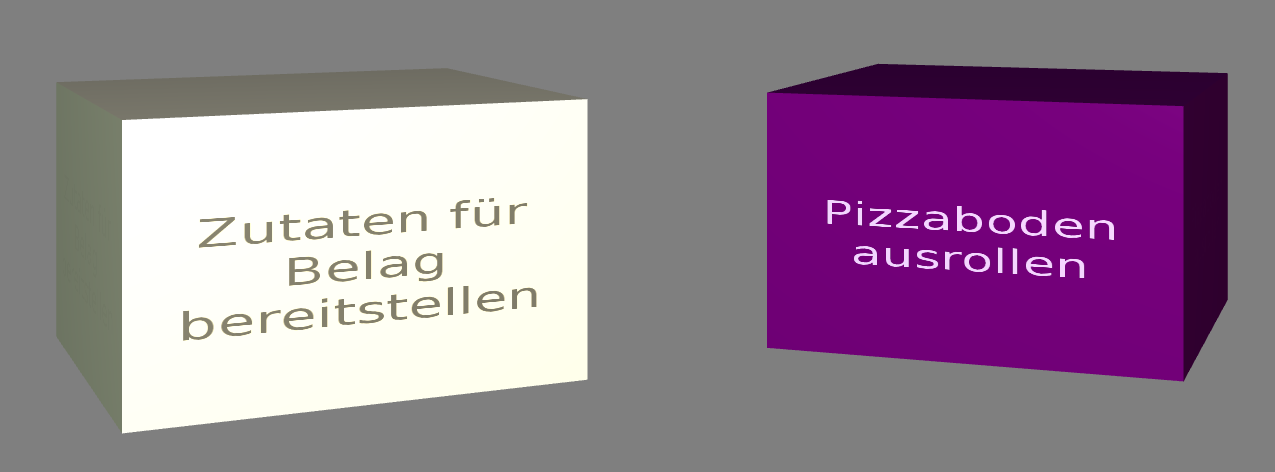
\includegraphics[width=16.5cm]{prozessknoten.png}
\caption{Zwei Prozessknoten; links im Ursprungszustand, rechts als angepasste Verwendung (Screenshot aus i\textgreater{}PM3D)}\label{visualisierung:prozessknoten}\end{figure}

Andererseits können Grafiken (Texturen) genutzt werden, um die Bedeutung eines Knotentyps zu visualisieren.
So steht ein Pluszeichen für einen AND-Connector, wie in \hyperref[visualisierung:and-connector]{Abbildung  \ref*{visualisierung:and-connector}} gezeigt wird.
\begin{figure}[htbp]
\centering
\capstart

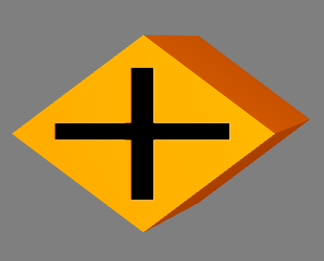
\includegraphics[height=8cm]{and_connector.png}
\caption{AND-Connector (Screenshot aus i\textgreater{}PM3D)}\label{visualisierung:and-connector}\end{figure}


\subsubsection{Blickwinkelabhängige Darstellung von Informationen}
\label{visualisierung:blickwinkelabhangige-darstellung-von-informationen}
Durch die freie Beweglichkeit und die Rotationsmöglichkeit der Kamera sowie der {\hyperref[ipm3d:ipm3d-visualisierung]{\emph{Objekte}}} (\autoref*{ipm3d:ipm3d-visualisierung}) ergeben sich sehr unterschiedliche Beobachtungsperspektiven.
Objekte können so von allen Seiten betrachtet werden.
Trotzdem soll sichergestellt werden, dass Texte oder Symbole auf den Objekten jederzeit erkennbar sind. Daher werden diese grundsätzlich auf allen Seiten dargestellt.
Jedoch führt dies bei bestimmten Drehpositionen zu störenden und möglicherweise verwirrenden Darstellungen, wenn beispielsweise bei einem Würfel zwei oder sogar drei Seiten zu sehen sind, die dasselbe anzeigen.

Um dies zu verbessern, werden die Seiten abhängig von Betrachtungswinkel dargestellt.
Wird eine Seite vom Benutzer weggedreht, wird die Schrift oder Textur nach und nach "`ausgeblendet"', indem die Vordergrundfarbe je nach Winkel mit der Hintergrundfarbe gemischt wird.
Ab einer gewissen Abweichung wird nur noch die Hintergrundfarbe angezeigt. So ist nur eine Seite deutlich zu erkennen und der Betrachter wird nicht durch die anderen Seiten abgelenkt.

\hyperref[visualisierung:schrift-uebergang]{Abbildung  \ref*{visualisierung:schrift-uebergang}} zeigt links den ungünstigsten Grenzfall, in dem alle Seiten gleich deutlich dargestellt werden. Dies ist der Fall, wenn der Betrachter direkt auf eine Ecke blickt.
Rechts ist der Knoten günstiger ausgerichtet und die Schrift ist auf der rechten Seite des Objekts kaum mehr zu erkennen.
\begin{figure}[htbp]
\centering
\capstart

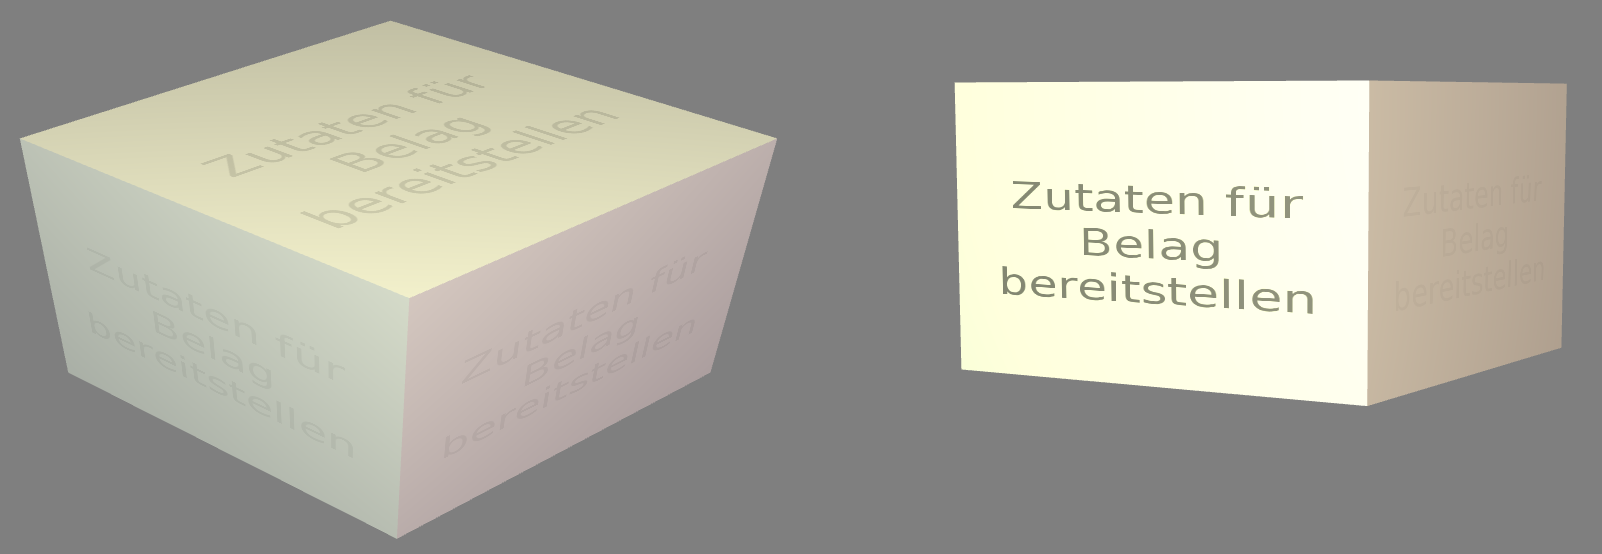
\includegraphics[width=16.5cm]{schrift-uebergang.png}
\caption{Schriftdarstellung bei direkter Sicht auf eine Ecke (links) und bei günstigerer Perspektive (Screenshot aus i\textgreater{}PM3D)}\label{visualisierung:schrift-uebergang}\end{figure}


\subsubsection{Berücksichtigung der Eingabemethoden}
\label{visualisierung:berucksichtigung-der-eingabemethoden}
Da i\textgreater{}PM3D nicht nur die klassischen Desktop-Bedienung mit Maus und Tastatur erlauben, sondern auch zur Evaluierung von neuartigen Eingabegeräten eingesetzt werden soll, müssen auch die Besonderheiten dieser Eingabemethoden berücksichtigt werden.
Die im Projekt verwendeten 3D-Eingabegeräte \cite{buchi} haben nur eine relativ begrenzte Genauigkeit bei der Auswahl und Platzierung von Objekten.
Vor allem ungeübten Benutzern kann es schwerfallen, Objekte zu selektieren und zu bewegen, besonders wenn die Objekte relativ klein sind.

Dies ist auch ein Grund, eine Graphdarstellung mit möglichst einfachen Objekten zu verwenden.
Es wird deswegen auch verzichtet, Elemente nach dem geometrischen Visualisierungsansatz ineinander zu schachteln, wie es bei 2D-Werkzeugen wie {\hyperref[grundlagen:mdf]{\emph{i\textgreater{}PM2}}} (\autoref*{grundlagen:mdf}) zu sehen war.
Es ist sinnvoll, Quader (oder annähernd quaderförmige Geometrien) einzusetzen, da Knoten in die physikalische Simulation eingebunden sind und Quader von der verwendeten Physikkomponente direkt unterstützt werden\footnote{
Von der Physikkomponente werden auch Kugeln unterstützt, allerdings ist die Verwendung von Quadern bisher fest in der Implementierung von i\textgreater{}PM3D vorgegeben.
}.
Die physikalische Simulation wird von den Eingabegeräten für die Selektion von Elementen genutzt, wie von \cite{buchi} beschrieben.


\subsection{Kanten}
\label{visualisierung:id2}\label{visualisierung:kanten}
Eine Kante sollte optisch leicht als Verbindung zwischen zwei Knoten erkannt werden können; außerdem muss ggf. visualisiert werden, welche Richtung die Kante besitzt.
In i\textgreater{}PM3D werden Kanten durch einen (in y-Richtung) gestreckten 3D-Quader dargestellt, der vom Startknoten bis zum Endknoten reicht.
Die Länge und Ausrichtung der Kanten wird automatisch angepasst, wenn die beteiligten Knoten im Raum verschoben werden.
Dies wird von der in \cite{uli} beschriebenen Editor-Komponente übernommen.

Die durch das Concept \code{TexturedConnection} (siehe {\hyperref[metamodelle:ebl]{\emph{Editor-Base-Level}}} (\autoref*{metamodelle:ebl})) bereitgestellte texturierte Verbindung dient dazu, gerichtete Kanten zu visualisieren.
Eine Möglichkeit ist es, eine Textur mit farblich vom Hintergrund abgehobenen Dreiecken zu verwenden, die so platziert sind, dass an zwei Ecken der Verbindung ein Pfeil entsteht.

\hyperref[visualisierung:gerichtete-verbindung]{Abbildung  \ref*{visualisierung:gerichtete-verbindung}} zeigt als Beispiel zwei Prozesse, die mit einem Kontrollfluss verbunden sind. Der Kontrollfluss läuft von "`Pizza backen"' nach "`Pizza verpacken"'.
\begin{figure}[htbp]
\centering
\capstart

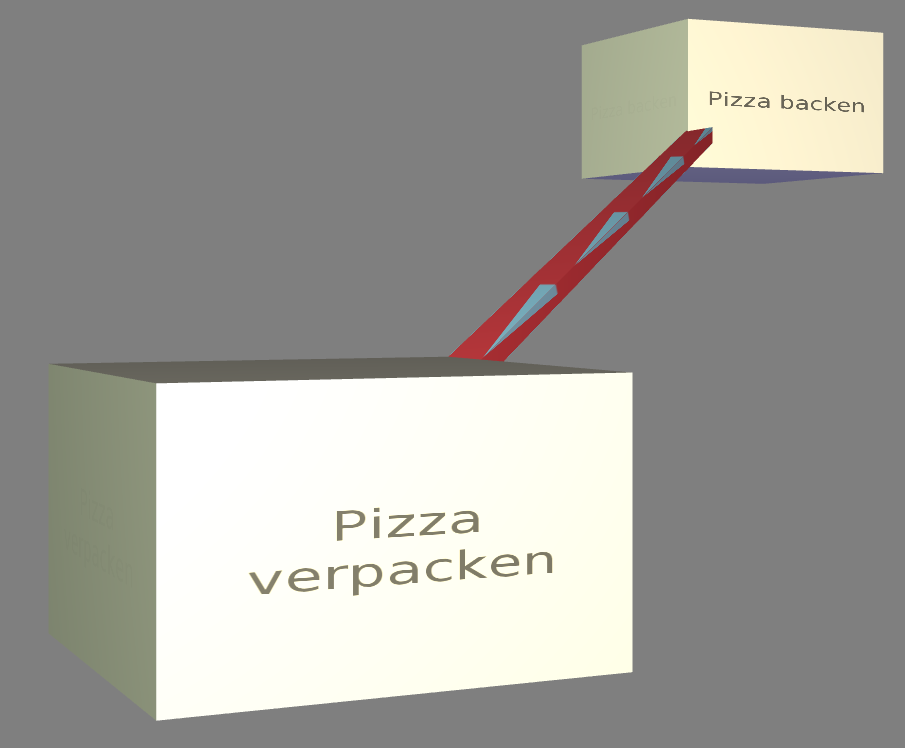
\includegraphics[height=8cm]{control_flow.png}
\caption{Gerichtete Kontrollflusskante von "`Backen"' nach "`Verpacken"' (Screenshot aus i\textgreater{}PM3D)}\label{visualisierung:gerichtete-verbindung}\end{figure}


\subsection{Szenenobjekte}
\label{visualisierung:szenenobjekte}
Zusätzlich zu den Elementen des eigentlichen Prozessmodells gibt es noch die Möglichkeit, beliebige 3D-Grafikobjekte in die Szene einzufügen, die im Editor-Metamodell als \code{SceneryObject} bezeichnet werden
(\emph{Anforderung (h)}).
Solche Szenenobjekte können zum Beispiel dafür eingesetzt werden, Abbilder von realen Objekten anzuzeigen.
Szenenobjekte können genauso wie Knoten, selektiert, frei bewegt, skaliert und rotiert werden. Sie besitzen aber sonst keine anderen Möglichkeiten, das Erscheinungsbild zu beeinflussen.


\section{Visualisierungsvarianten für interaktive Modelleditoren}
\label{visualisierung:visualisierungsvarianten}\label{visualisierung:visualisierungsvarianten-fur-interaktive-modelleditoren}
Da die hier vorgestellte Visualisierung in einem interaktiven Modelleditor eingesetzt wird, ergibt sich noch die Anforderung, Visualisierungsvarianten der Modellelemente zu unterstützen.
So sollen Interaktionen des Benutzers mit den Modellobjekten sichtbar gemacht werden, indem die Visualisierung der Objekte temporär verändert wird.
Diese Modifikationen werden nicht im Editor-Usage-Model persistiert; daher werden alle Objekte im Normalzustand angezeigt nachdem ein Modell neu geladen wurde.


\subsection{Hervorhebung}
\label{visualisierung:hervorhebung}\label{visualisierung:id3}
Diese Variante wird dafür eingesetzt, ein Objekt kurzzeitig beim Überfahren durch einen Cursor eines Eingabegeräts hervorzuheben.
Dargestellt wird das abhängig von der Helligkeit der Grundfarbe des Objekts durch eine Aufhellung bzw. einer Abdunkelung der Farbe. Der Farbton wird dabei nicht verändert.
\hyperref[visualisierung:hervorhebung-sc]{Abbildung  \ref*{visualisierung:hervorhebung-sc}} zeigt im Vergleich ein hervorgehobenes Datenelement und eines im Normalzustand (rechts).
\begin{figure}[htbp]
\centering
\capstart

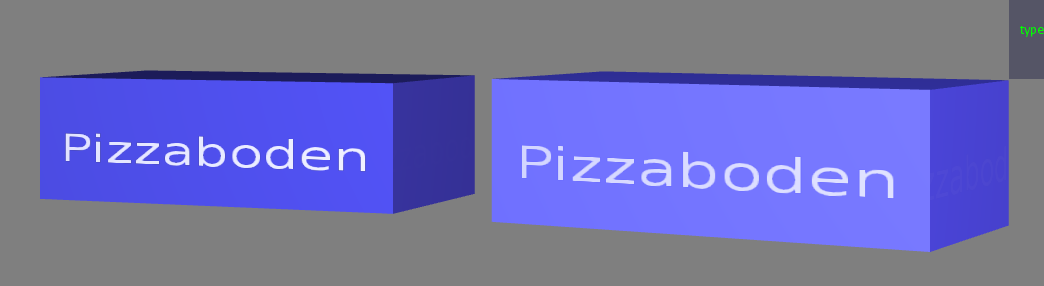
\includegraphics[width=16.5cm]{dataitems_hervorhebung.png}
\caption{Datenknoten, normal (links) und hervorgehoben (Screenshot aus i\textgreater{}PM3D)}\label{visualisierung:hervorhebung-sc}\end{figure}


\subsection{Selektion}
\label{visualisierung:selektion}
Prozessmodellelemente und Szenenobjekte können durch den Benutzer ausgewählt werden.
Selektierte Objekte sollen von unselektierten Objekten auch bei großer Entfernung und ungünstigen Blickwinkeln unterscheidbar sein, wobei aber jederzeit noch erkennbar sein muss, um welche Art von Modellelement es sich handelt.

Die Visualisierung des Selektionszustandes soll daher möglich auffällig sein, ohne das Erscheinungsbild allzu stark zu beeinflussen.
Um die Selektion von der Hervorhebung unterscheidbar zu machen, wird für die Selektion der Rand des Objekts in der Komplementärfarbe eingefärbt. Die Definition des "`Rands"' ist je nach Objekttyp unterschiedlich\footnote{
Der Rand ist über die Texturkoordinaten definiert. {\hyperref[renderbib:erweiterung-interaction]{\emph{Siehe}}} (\autoref*{renderbib:erweiterung-interaction}).
}.
In \hyperref[visualisierung:selektion-sc]{Abbildung  \ref*{visualisierung:selektion-sc}} sind zwei selektierte Knoten zu sehen.
\begin{figure}[htbp]
\centering
\capstart

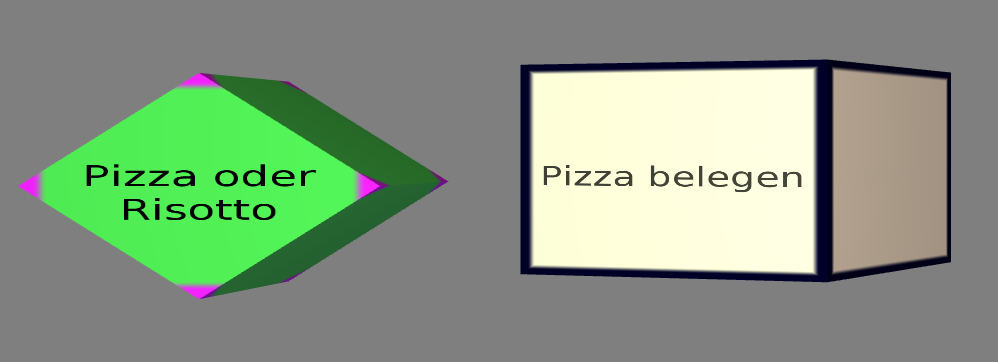
\includegraphics[width=16.5cm]{selektierte_knoten.png}
\caption{Entscheidungsknoten und Prozess im selektierten Zustand (Screenshot aus i\textgreater{}PM3D)}\label{visualisierung:selektion-sc}\end{figure}


\subsection{Deaktivierung}
\label{visualisierung:deaktivierung}\label{visualisierung:id5}
Objekte können durch den Modelleditor deaktiviert werden. Welche Bedeutung dies hat, wird vom Editor festgelegt.
Zur Visualisierung dieses Zustandes wird das Objekt transluzent in einem Grauton dargestellt, der von der normalen Farbe abhängig ist.
So kann man auch Elemente erkennen, die hinter dem deaktivierten liegen und von diesem verdeckt werden.
\hyperref[visualisierung:deaktivierung-sc]{Abbildung  \ref*{visualisierung:deaktivierung-sc}} zeigt einen deaktivierten Prozess, hinter dem sich ein anderer Prozess befindet.
\begin{figure}[htbp]
\centering
\capstart

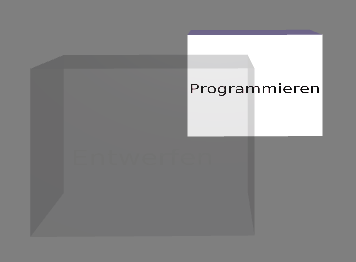
\includegraphics[height=7cm]{prozesse_deaktiviert.png}
\caption{Deaktivierter (vorne, durchsichtig) und aktivierter Prozess (Screenshot aus i\textgreater{}PM3D)}\label{visualisierung:deaktivierung-sc}\end{figure}

Die drei gezeigten Visualisierungsvarianten können frei kombiniert werden.
So ist es möglich, ein gleichzeitig hervorgehobenes, selektiertes und deaktiviertes Modellelement darzustellen.


\section{2D-Modellierungsflächen}
\label{visualisierung:d-modellierungsflachen}\label{visualisierung:modellierungsflaechen}
Für eine übersichtliche Darstellung des Prozessmodells ist es häufig erwünscht, Elemente in einer bestimmten Weise anzuordnen.
Zur Vereinfachung der Platzierung werden in 2D-Modellierungswerkzeugen oft im Hintergrund dargestellte Gitter genutzt, die eine optische Hilfe darstellen.
Noch hilfreicher können "`magnetische"' Gitter sein, die grob in der Nähe platzierte Objekte automatisch auf feste, regelmäßige Positionen verschieben.

Um dies zu erreichen, wird die {\hyperref[ipm3d:mod-simx]{\emph{Physikkomponente}}} (\autoref*{ipm3d:mod-simx}) genutzt.
Sobald sich ein Objekt nahe genug an einer solchen 2D-Modellierungsfläche befindet, wird es nach dem Loslassen durch den Benutzer (Deselektion) von der "`Gravitation"' der Ebene angezogen.
Das Objekt bewegt sich solange, bis dessen Mittelpunkt die Fläche erreicht hat und dort automatisch angehalten wird.
Näheres zur Implementierung dieser "`Gravitationsflächen"' findet sich in \cite{buchi}.

Grafisch werden diese Flächen transluzent dargestellt, wobei darauf Gitterlinien zu erkennen sind.
Diese Linien haben allerdings keine physikalische Bedeutung, sondern dienen nur als optische Platzierungshilfe.

\hyperref[visualisierung:modellierungsflaeche]{Abbildung  \ref*{visualisierung:modellierungsflaeche}} zeigt zwei solcher Flächen ober- und unterhalb des Betrachters.
\begin{figure}[htbp]
\centering
\capstart

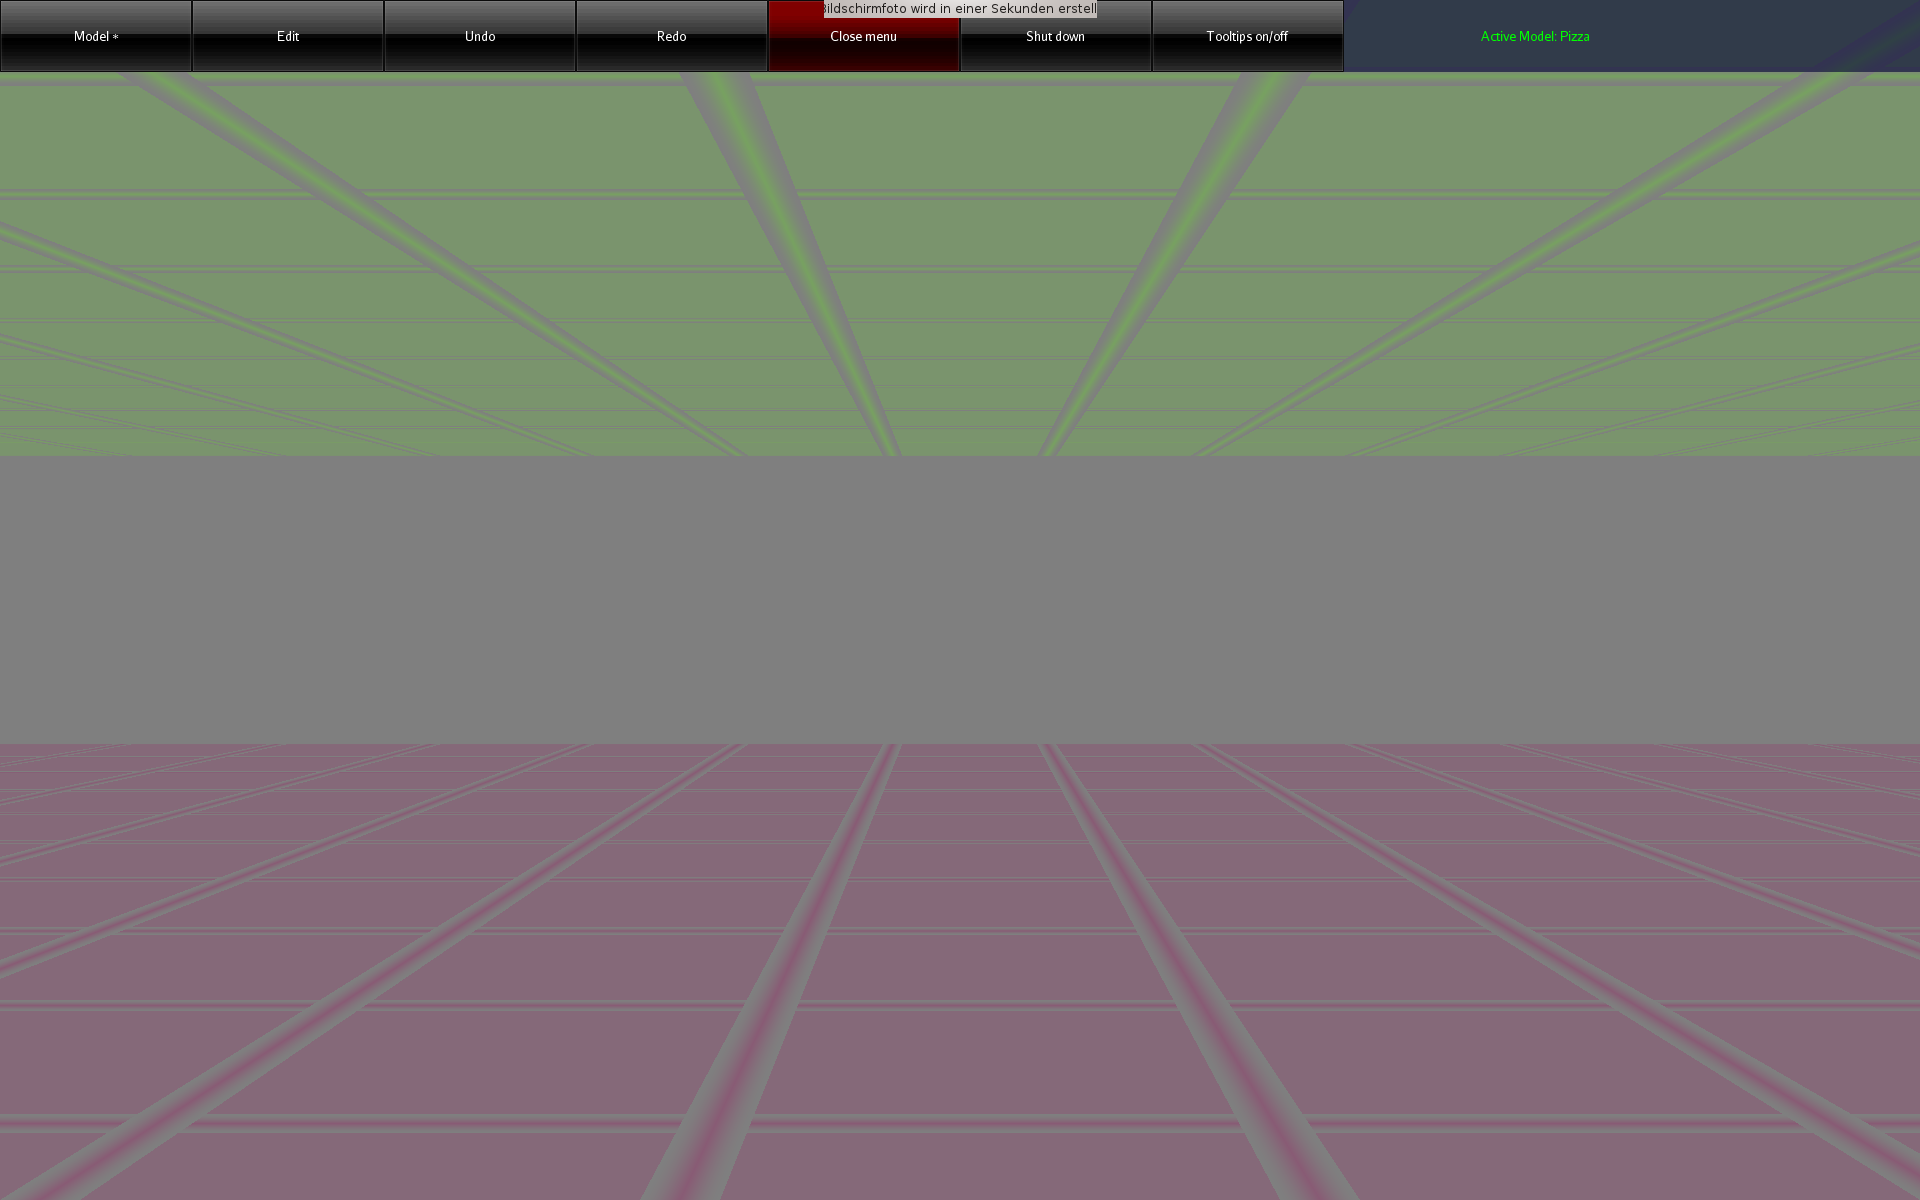
\includegraphics[width=16cm]{flaechen.png}
\caption{Zwei leere Modellierungsflächen (Screenshot aus i\textgreater{}PM3D)}\label{visualisierung:modellierungsflaeche}\end{figure}


\section{Beleuchtung}
\label{visualisierung:id6}\label{visualisierung:beleuchtung}
Für die Beleuchtung der Szene werden mehrere Lichtquellen eingesetzt. Die primäre Lichtquelle befindet sich direkt an der Kamera und bewegt sich mit dieser.
Die Lichtfarbe ist weiß, also wird der Farbton der beleuchteten Objekte unverfälscht dargestellt.

Zur Verbesserung der Orientierung befindet sich jeweils eine weniger intensive, farbige Lichtquelle an drei festen Positionen unterhalb (blau), links (grün) und rechts (rot) der Szene, von der Startposition der Kamera aus gesehen.
So soll es für den Benutzer leichter zu erkennen sein, welche Seite der Objekte in Bezug auf die Ausgangsposition nach unten, links beziehungsweise nach rechts zeigt.

Die von der {\hyperref[renderbib:render-bibliothek]{\emph{Render-Bibliothek}}} (\autoref*{renderbib:render-bibliothek}) bereitgestellten Lichtquellen nach dem Phong-Lichtmodell \cite{phong_illumination_1975} sorgen für eine relativ realistische Beleuchtung bei vertretbarem Rechenaufwand.
Für die Visualisierung von 3D-Graphmodellen stellt sich die Frage, wie die Lichtparameter am besten gewählt werden sollten, um eine möglichst hohe Lesbarkeit und eine gute Orientierung im Raum zu ermöglichen.

Im Phong-Lichtmodell wird das von einem Objekt reflektierte Licht in drei Beiträge unterschieden \cite{akenine-moller_real-time_2008}.

Der Hauptanteil des reflektierten Lichts wird im Normalfall vom \emph{diffuse}-Anteil beigesteuert, welcher abhängig vom Winkel zur Lichtquelle ist.
Von der Lichtquelle eher abgewandte Seiten erscheinen daher dunkel, was sich ungünstig auf die Erkennbarkeit von Informationen auswirken kann.

Um dies auszugleichen, kann der \emph{ambient}-Anteil (Umgebungslicht) erhöht werden, der vom Winkel unabhängig ist.
Wird dieser zu hoch gesetzt, leidet allerdings der räumliche Eindruck.

Der \emph{specular}-Anteil erzeugt spiegelnde Reflexionen auf Objekten, die auch von der Betrachterposition relativ zum Objekt abhängen.
Dieser Anteil kann folglich die räumliche Orientierung unterstützen.
Allerdings führt die starke Aufhellung an bestimmten Stellen dazu, dass sich Text dort schlecht ablesen lässt.

Außerdem kann bei (OpenGL)-Lichtquellen noch angegeben werden, wie stark die Helligkeit mit steigender Entfernung von der Lichtquelle abfällt.
Hierdurch kann der Tiefeneindruck verbessert werden.

Ein starker Abfall der Beleuchtung führt aber zu Problemen, wenn gleichzeitig Objekte mit Text in der Nähe der Lichtquelle und weit entfernt in lesbarer Form dargestellt werden sollen.
Objekte in der Nähe werden zu hell dargestellt, während weit entfernte Objekte zu dunkel sind.
Genauso ergibt sich bei gerichteten Verbindungen, die sich weit im Hintergrund befinden, das Problem, dass die darauf abgebildeten Richtungsmarkierungen schlecht zu erkennen sind.

Insgesamt hat sich bei Versuchen gezeigt, dass es schwierig ist, die Lichtparameter so zu setzen, dass eine in allen Situationen brauchbare Beleuchtung entsteht.


\section{Visualisierung eines Beispielsprozesses}
\label{visualisierung:vis-beispiel}\label{visualisierung:visualisierung-eines-beispielsprozesses}
\hyperref[visualisierung:beispielprozess-screenshot]{Abbildung  \ref*{visualisierung:beispielprozess-screenshot}} zeigt den in i\textgreater{}PM3D modellierten Prozess "`Pizza produzieren"'.
Zusätzlich zu den bisher gezeigten Knoten ist hier noch der Start-/Stop-Knoten – als roter, abgerundeter Quader dargestellt – zu sehen.
Neben der funktionalen Perspektive, vertreten durch die Start-Stop-Knoten, Prozessknoten und zwei AND-Konnektoren, wird auch die Datenperspektive mit Datenknoten und dazwischen verlaufenden Datenflüssen dargestellt.
Die Abbildung zeigt, wie sich durch das Deaktivieren von Knoten ein Teil des Modells (hier der Datenperspektive) ausblenden lässt, um die Ansicht auf momentan interessante Teile zu fokussieren und die Übersichtlichkeit zu erhöhen.
Aktiviert ist nur der Datenfluss der Pizza selbst, von "`Pizza belegen"' bis hin zum Ende des Prozesses; die restlichen Datenknoten und damit auch die dazwischenliegenden Verbindungen sind deaktiviert.
Die dünnen, blauen Kanten zwischen den Prozessen und Datenknoten stellen \code{NodeDataConnections} dar, welche \code{Nodes} und \code{DataItems} des Prozessmodells miteinander assoziieren.
\begin{figure}[htbp]
\centering
\capstart

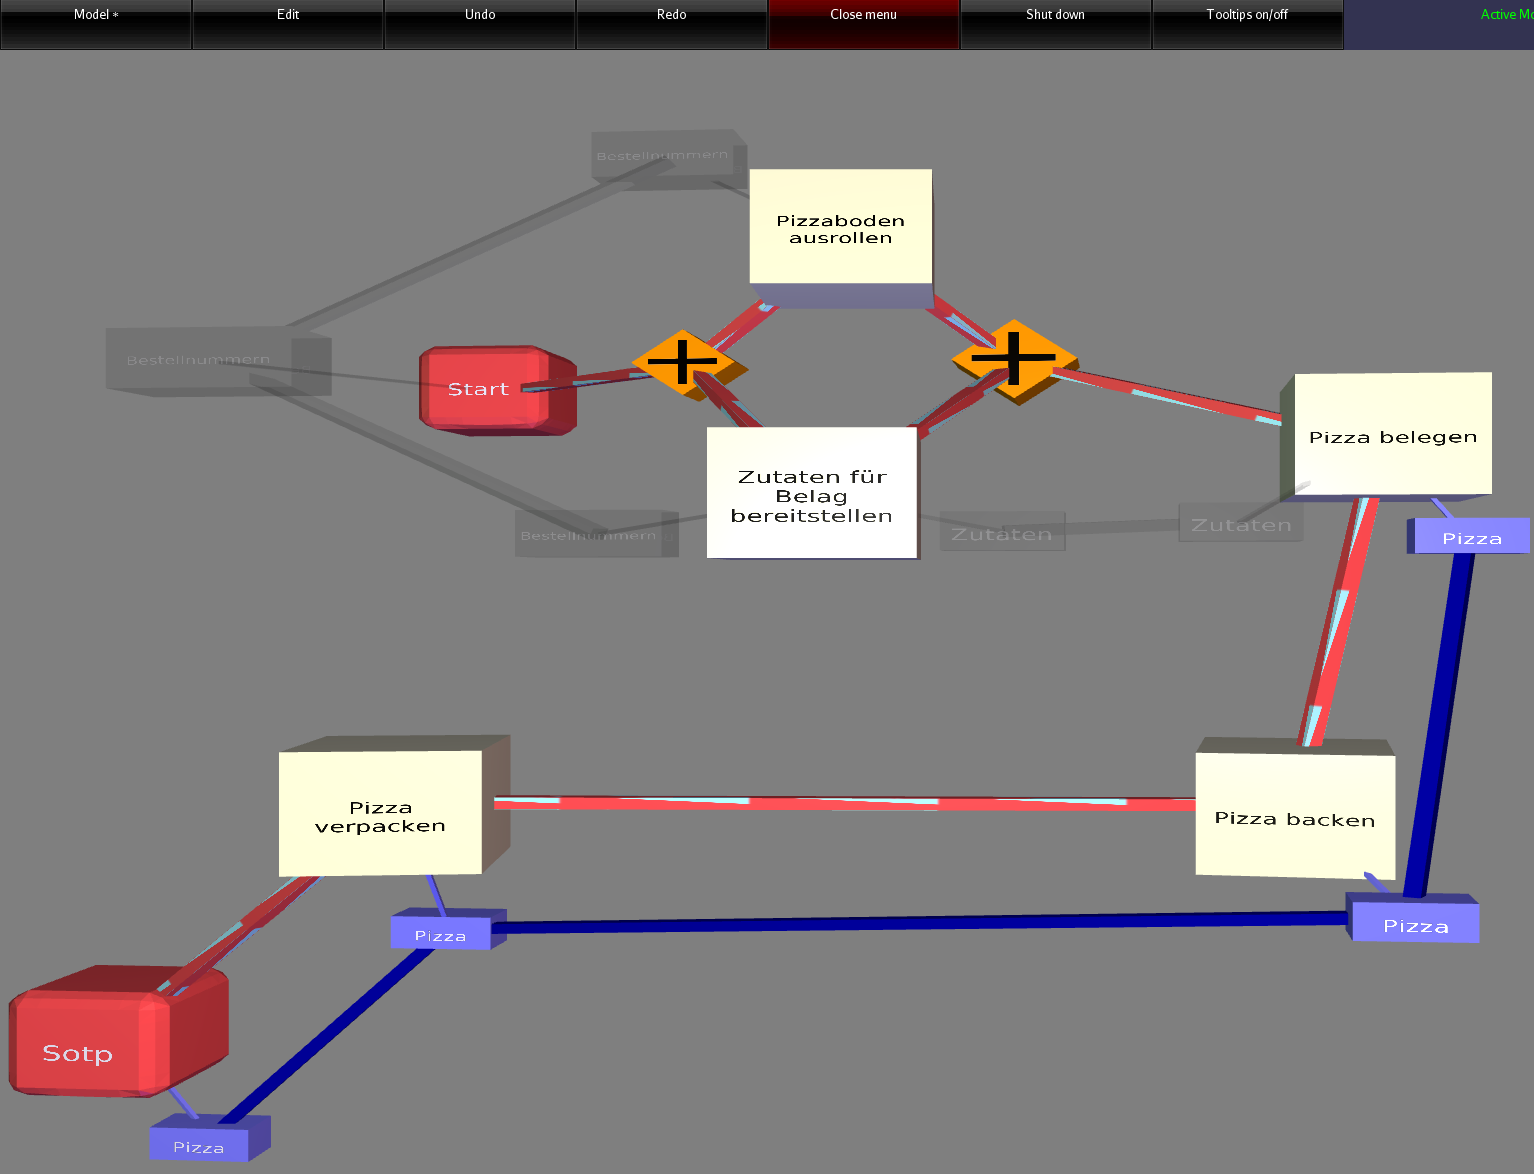
\includegraphics[width=17cm]{gesamt2.png}
\caption{Beispiel für einen Prozess mit deaktivierten Datenfluss-Elementen (Screenshot aus i\textgreater{}PM3D)}\label{visualisierung:beispielprozess-screenshot}\end{figure}


\section{Umsetzung von verschiedenen Nutzungsmöglichkeiten der dritten Dimension}
\label{visualisierung:vis-umsetzung}\label{visualisierung:umsetzung-von-verschiedenen-nutzungsmoglichkeiten-der-dritten-dimension}
In diesem Abschnitt soll gezeigt werden, welche {\hyperref[related:related-zusammenfassung]{\emph{in}}} (\autoref*{related:related-zusammenfassung}) genannen Nutzungsmöglichkeiten sich mit dem bisherigen Prototypen umsetzen lassen oder welche Erweiterungen dafür vorgenommen werden sollten.
Die folgende Tabelle zeigt hierzu eine Übersicht über verschiedene Verwendungen der dritten Dimension und deren Umsetzung in i\textgreater{}PM 3D, welche anschließend näher ausgeführt wird.

\begin{DUlineblock}{0em}
\item[] 
\end{DUlineblock}
\begin{tabular}{|c|c|}
\hline
3. Dimension verwendet für & aktuell umsetzbar in i>PM3D?\tabularnewline
\hline
\hline
unterschiedl. Beziehungstypen & ja\tabularnewline
\hline
Darstellung von Modellattributen & ja, aber manuelle Platzierung nötig\tabularnewline
\hline
Zeitachse & ja, aber manuelle Platzierung nötig. 2D-Flächen als Swimlanes\tabularnewline
\hline
mehrere / hierarchische Modelle & ja, aber ohne Verbindungen zw. den Modellen\tabularnewline
\hline
mehrere Modelltypen & nein\tabularnewline
\hline
Einbettung in virtuelle Umgebung & ja, aber ohne Animation\tabularnewline
\hline
\end{tabular}
\begin{DUlineblock}{0em}
\item[] 
\end{DUlineblock}


\subsection{Visualisierung von Attributen}
\label{visualisierung:visualisierung-von-attributen}
Welche Information durch den Abstand (die "`Tiefe"') vermittelt werden soll, wird durch den Benutzer festgelegt.
Durch die freie Platzierbarkeit lässt sich prinzipiell jede gewünschte geometrische Anordnung erreichen.
Elemente nach ihrer Wichtigkeit anzuordnen, wie es {\hyperref[related:related]{\emph{in}}} (\autoref*{related:related}) vorgeschlagen wurde, ist damit möglich.
Außerdem lassen sich durch unterschiedliche Entfernung der Knoten von einem Fixpunkt beliebige Attribute aus dem Prozessmodell visualisieren.

Allerdings ist der Nutzen dadurch eingeschränkt, dass der Benutzer die Positionierung der Elemente manuell vornehmen muss.
Bei einer Änderung der Attribute muss auch die Tiefen-Visualisierung entsprechend angepasst werden. Dies ist allerdings aufwändig und fehleranfällig.
Um dies für den Anwender effizient zu gestalten, müssten Algorithmen integriert werden, welche die Platzierung anhand von Attributwerten aus dem Prozessmodell automatisch übernehmen und die Visualisierung auch bei Änderungen am Prozessmodell zur Laufzeit synchron halten.

Eine gewisse Hilfe, besonders für diskrete Attribute, können die 2D-Modellierungsflächen darstellen. So kann jeder Fläche ein bestimmter Wert zugewiesen werden.
Alle Elemente, die diesen Wert aufweisen, werden auf der passenden Fläche platziert.
Die Fläche unterstützt den Benutzer bei der Anordnung, indem sie die Objekte automatisch in einer Ebene platziert, wenn sie in der Nähe der Fläche abgelegt werden.
Um Objekte beispielsweise in die Kategorien "`wichtig"' und "`unwichtig"' einzuteilen, ließen sich zwei (parallele) Flächen definieren, anhand derer die Objekte sortiert werden könen.
Da bisher nur die Platzierung senkrecht zur Fläche automatisch erfolgt, sollte in einer Erweiterung von i\textgreater{}PM3D die Möglichkeit hinzugefügt werden, 2D-Layout-Algorithmen anzuwenden, um beispielsweise Knoten mit bestimmten Eigenschaften zu gruppieren oder für eine kreuzungsfreie Darstellung der Verbindungen in der Ebene zu sorgen.


\subsection{Zeitliche Abläufe}
\label{visualisierung:zeitliche-ablaufe}
Eine weitere Nutzungsmöglichkeit für die dritte Dimension ist die Darstellung von zeitlichen Abläufen.
Diese werden in einem Prozess üblicherweise schon durch den Kontrollfluss grob vorgegeben, allerdings lassen sich gewisse Aspekte mit einer sinnvollen 3D-Anordnung weiter betonen.
Die Zeitdauer lässt sich durch die Entfernung zwischen Prozessknoten visualisieren.
Einerseits lassen sich Prozesschritte, die (nahezu) gleichzeitig ausgeführt werden, und zugehörige Knoten – wie assoziierte Daten – gemeinsam auf einer 2D-Ebene darstellen, ähnlich wie es von {\hyperref[related:gil]{\emph{Gil}}} (\autoref*{related:gil}) anhand von 3D-UML-Sequenzdiagrammen gezeigt wurde.
Andererseits kann man 2D-Ebenen als "`Swimlanes"' nutzen, wie sie aus BPMN bekannt sind.
Dazu werden Prozessschritte auf parallel verlaufenden Flächen gruppiert, die zu einer bestimmten ausführenden Entität gehören.


\subsection{Veranschaulichung von Beziehungen}
\label{visualisierung:veranschaulichung-von-beziehungen}
Durch die Anordnung der Elemente die Bedeutung von Beziehungen zu unterstreichen ist ebenfalls möglich, wobei wiederum die 2D-Flächen hilfreich sind.
So kann durch die Positionierung der Knoten auf einer Fläche leicht verdeutlicht werden, dass Kanten, die parallel zur Fläche verlaufen, eine andere Bedeutung haben als diejenigen, die aus der Ebene herausragen und zu Elementen führen, die auf einer anderen Fläche platziert sein können.
{\hyperref[related:gef3d]{\emph{In}}} (\autoref*{related:gef3d}) wurde dies genutzt, um gleichzeitig Beziehungen innerhalb eines Modells als auch Beziehungen zu Elementen eines anderen Modells (möglicherweise auch anderen Typs) zu visualisieren.
i\textgreater{}PM 3D hat die Fähigkeit, mehrere Modelle gleichzeitig zu laden, allerdings werden Verbindungen zwischen mehreren Modellen und verschiedene Modelltypen zur gleichen Zeit noch nicht unterstützt ({\hyperref[modellanbindung:modellanbindung]{\emph{siehe}}} (\autoref*{modellanbindung:modellanbindung})).
Dies sollte in einer weiteren Entwicklung vorrangig hinzugefügt werden, um diese Anwendung der dritten Dimension zu erlauben, welche deutliche Vorteile zu 2D-Darstellungen verspricht.


\subsection{Hierarchische Darstellung und mehrere Modelle}
\label{visualisierung:hierarchische-darstellung-und-mehrere-modelle}
Die Visualisierung von hierarchischen Diagrammen in derselben 3D-Szene ist für die Darstellung von kompositen Prozessen hilfreich.
Ein Verfeinerungsmodell sollte in einem separaten Modell abgelegt werden, welches im grobgranularen Modell durch einen kompositen Prozessknoten vertreten wird.
Wird das Verfeinerungsmodell nach Bedarf "`ausgeklappt"', sollte eine optische Verbindung zum Knoten im übergeordneten Modell die Zusammengehörigkeit anzeigen, wie es beispielsweise von {\hyperref[related:mcintosh]{\emph{McIntosh}}} (\autoref*{related:mcintosh}) gezeigt wurde.
Dies ist noch nicht möglich, da Verbindungen zwischen Modellen nicht erlaubt sind.
Durch die Fähigkeit von i\textgreater{}PM3D, manuell mehrere Modelle laden zu können \cite{uli}, lassen sich solche Hierarchiestufen immerhin schon in separaten Modellen ablegen und in derselben 3D-Szene anzeigen.
Weiterhin wäre eine direkte Unterstützung durch den Editor angebracht, welcher die Subdiagramme bei einer Benutzerinteraktion mit dem kompositen Prozessknoten automatisch öffnen sollte.

Da sich der Benutzer frei in der Szene bewegen kann, können unterschiedliche Betrachtungsperspektiven eingenommen werden.
Die Perspektive kann so gewählt werden, dass die momentan für den Benutzer besonders interessanten Aspekte der 3D-Szene deutlich zu erkennen sind.
Besonders hilfreich ist dies, wenn mehrere Modelle gleichzeitig dargestellt werden.
Werden beispielsweise zwei Modelle angezeigt, wobei das eine aktuell im Vordergrund dargestellt wird und das andere im Hintergrund liegt, ist das Modell im Vordergrund wegen des geringeren Abstands zum Benutzer besser zu erkennen.
\hyperref[visualisierung:zweimodelle-vorne]{Abbildung  \ref*{visualisierung:zweimodelle-vorne}} zeigt diese Situation.
Soll nun das andere Modell genauer betrachtet werden, kann dies erreicht werden, indem die Szene einfach von hinten betrachtet wird.
\hyperref[visualisierung:zweimodelle-hinten]{Abbildung  \ref*{visualisierung:zweimodelle-hinten}} stellt dieselben Modelle dar, allerdings hat sich der Benutzer erst um 180° gedreht und dann etwas nach hinten bewegt, um das Modell mit den blauen Prozessknoten zu fokussieren.

Die andere Möglichkeit ist, dass sich der Benutzer zum blauen Modell hinbewegt, wobei das gelbe dann hinter dem Benutzer liegt und nicht mehr zu sehen ist.
\begin{figure}[htbp]
\centering
\capstart

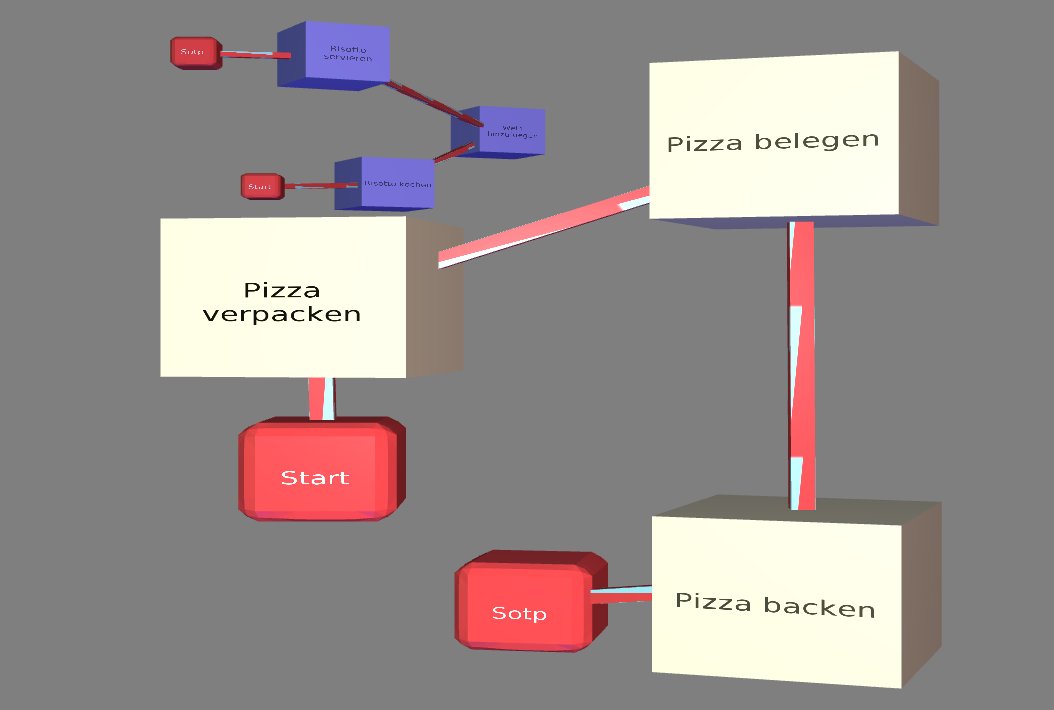
\includegraphics[width=16.5cm]{zweimodelle-vorne.png}
\caption{Darstellung von zwei Prozessen, Fokus auf gelbem Modell (Screenshot aus i\textgreater{}PM3D)}\label{visualisierung:zweimodelle-vorne}\end{figure}
\begin{figure}[htbp]
\centering
\capstart

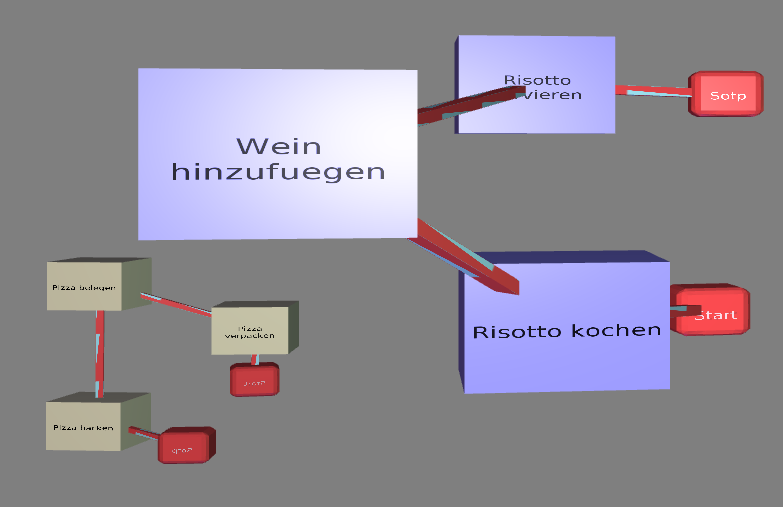
\includegraphics[width=16.5cm]{zweimodelle-hinten.png}
\caption{Darstellung von zwei Prozessen, Fokus auf blauem Modell (Screenshot aus i\textgreater{}PM3D)}\label{visualisierung:zweimodelle-hinten}\end{figure}


\subsection{Einbettung in eine virtuelle Umgebung}
\label{visualisierung:einbettung-in-eine-virtuelle-umgebung}
Durch die Möglichkeit, mittels Szenenobjekten beliebige 3D-Objekte einzubinden, lässt sich der Prozessgraph in eine virtuelle Ausführungsumgebung einbetten.
Die Szenenobjekte können in i\textgreater{}PM3D aus COLLADA-Dateien geladen werden, welche von Anwendungen wie beispielsweise \emph{Blender} \cite{www:blender} erstellt werden können.
So lässt sich grundsätzlich jede beliebige 3D-Szene aus einzelnen Objekten aufbauen, um die {\hyperref[related:informations-integration]{\emph{in}}} (\autoref*{related:informations-integration}) gezeigten Nutzungsmöglichkeiten zu realisieren.

Durch den modularen Aufbau des Systems auf Basis von Simulator X ist die Integration weiterer Funktionalität durch die Implementierung einer neuen Komponente einfach möglich.
Bewegungsanimationen von Szenenobjekten – beispielsweise Werkstücken – sind bisher noch nicht integriert. Um dies nachzurüsten, müsste eine "`Animationskomponente"' implementiert werden.
Eine solche Komponente könnte Objekte automatisch oder vom Benutzer gesteuert (bspw. durch ein Kommando "`zum nächsten Datenknoten bewegen"') entlang von Datenflüssen bewegen und so die Dynamik des Prozessablaufs veranschaulichen.
Für {\hyperref[metamodelle:ebl-figures]{\emph{Szenenobjekte}}} (\autoref*{metamodelle:ebl-figures}) kann eine physikalische Repräsentation in Form eines Quaders oder einer Kugel definiert werden, um diese in die Physiksimulation aufzunehmen.
Dies kann durch eine Animationskomponente genutzt werden, um Kollisionen zwischen bewegten Szenenobjekten zu erkennen.
Eine andere Möglichkeit ist die Integration von Komponenten, die automatische Pfadsuch-Algorithmen wie beispielsweise den A*-Algorithmus \cite{hart_correction_1972} anwenden, welche unter anderem dazu genutzt werden können, optimale Laufwege zu finden.


\section{Weitere Entwicklungsmöglichkeiten}
\label{visualisierung:weitere-entwicklungsmoglichkeiten}\label{visualisierung:vis-entwicklungsmoeglichkeiten}
Die momentan umgesetzte Visualisierung von Prozessen zeigt nach unserer\footnote{
Damit sind der Autor dieser Arbeit und \cite{uli} sowie \cite{buchi} gemeint.
} Ansicht, dass eine 3D-Ansicht auf Prozessdiagramme durchaus praktikabel ist.
Es zeigten sich bei ersten Versuchen mit dem i\textgreater{}PM3D Prototypen einige Probleme in Hinblick auf die Visualisierung, die teilweise schon angesprochen wurden oder im Folgenden noch erwähnt werden.

Um die Darstellung zu verbessern und den Nutzen für den Anwender weiter zu erhöhen, gibt es eine Vielzahl von Entwicklungsmöglichkeiten.
Hier sollen vor allem einige dargestellt werden, die sich aus den Erfahrungen mit dem Prototypen ergeben haben und die auf Basis des momentanen Projektstands ohne grundlegende Veränderungen umgesetzt werden können.


\subsection{Darstellung von Text}
\label{visualisierung:darstellung-von-text}
Die {\hyperref[renderbib:schrift-rendering]{\emph{Render-Bibliothek}}} (\autoref*{renderbib:schrift-rendering}) stellt Text dar, indem dieser in ein 2D-Bild geschrieben und so als Textur auf dem Objekt angezeigt wird.

Andere Techniken, die eine höhere Darstellungsqualität erreichen, wie sie beispielsweise von {\hyperref[related:gef3d]{\emph{GEF3D}}} (\autoref*{related:gef3d}) genutzt oder von \cite{ray_vector_2005} vorgestellt werden, wurden ebenfalls in Betracht gezogen.
Besonders die Möglichkeiten aktuellster Grafikhardware mit OpenGL4-Unterstützung, neue Geometrien direkt auf der Grafikeinheit per Tesselation-Shader zu erzeugen, könnten für die Implementierung von gut lesbaren und dennoch performanten Darstellungstechniken interessant sein.

Jedoch war die Schriftqualität des verwendeten texturbasierten Ansatzes ausreichend für den hier entwickelten Prototypen und lies sich einfach implementieren.
Da die Darstellung von Schrift wichtig für Verständlichkeit und Nutzen der grafischen Repräsentation ist, sollte für weitere Arbeiten auf diesem Gebiet jedoch evaluiert werden, inwieweit sich die Qualität des hier genutzten Ansatzes verbessern lässt oder ob ein anderer Ansatz gewählt werden muss.

Bei ungünstigen Beobachtungssituationen, also bei großer Entfernung und schräger Betrachtung von Flächen, wird es im Prototypen schnell schwierig, Texte ohne Anstrengung zu lesen.
Es müssen eher große Schriften gewählt werden und daher lässt sich relativ wenig Information auf den Knoten darstellen.
Außerdem muss der Kontrast zwischen Textfarbe und Hintergrund immer sehr hoch sein, um eine angemessene Lesbarkeit zu erreichen. Eine bessere Darstellungsqualität würde hier für mehr Flexibilität sorgen.

Eine sinnvolle Erweiterungsmöglichkeit wäre es, die Anzeige von Informationen bei weit entfernten Objekten automatisch zu vereinfachen\footnote{
In der Computergrafik wird das Prinzip als "`Level Of Detail"' bezeichnet.
}, indem beispielsweise ein Text abgekürzt und größer dargestellt wird.
So wäre es möglich, Knoten mit größerem Abstand immerhin noch zu unterscheiden.
Dafür kann ein zusätzliches Attribut im Prozessmodell definiert werden, dass eine Abkürzung für ein längeres Textattribut angibt.


\subsection{Konfigurierbarkeit}
\label{visualisierung:konfigurierbarkeit}
Abgesehen von den im {\hyperref[metamodelle:ebl]{\emph{Metamodell}}} (\autoref*{metamodelle:ebl}) konfigurierbaren Visualisierungsparametern fehlt es noch an weiteren Möglichkeiten, die grafische Darstellung zu beeinflussen.

So wäre es angebracht, eine Konfigurationsmöglichkeit für die {\hyperref[visualisierung:beleuchtung]{\emph{Beleuchtung}}} (\autoref*{visualisierung:beleuchtung}) anzubieten.
Wie in jenem Abschnitt gesagt ist es schwierig, Einstellungen zu finden, die für alle Situationen gut geeignet sind.
Diese hängen auch von der verwendeten Anzeige und von Einflüssen wie Umgebungslicht oder der persönlichen Wahrnehmung des Benutzers ab.

In der grafischen Oberfläche sollte es hierzu eine Möglichkeit geben, Lichtquellen zu setzen und deren Parameter zu verändern.
Es bietet sich an, auch sinnvolle Standardeinstellungen bzw. auswählbare Profile zur Verfügung zu stellen, um den Benutzer nicht mit zu vielen Aufgaben zu überfordern.
Lichtquellen sind in Simulator X über zugehörige Licht-Entities erstell- und konfigurierbar, wie es auch von der {\hyperref[renderkomponente:renderkomponente]{\emph{Renderkomponente}}} (\autoref*{renderkomponente:renderkomponente}) unterstützt wird.

Ähnliches gilt für {\hyperref[visualisierung:modellierungsflaechen]{\emph{2D-Modellierungsflächen}}} (\autoref*{visualisierung:modellierungsflaechen}). Sie sind momentan in der Implementierung fest vorgegeben, da es in der GUI noch keine Konfigurationsmöglichkeit gibt.
Die Flächen können aber ebenfalls nach Bedarf erstellt und über zugehörige Entities konfiguriert werden.

Es wäre sinnvoll, die aktuellen Einstellungen für Lichtquellen und Modellierungsflächen auch in die Editor-Modelle aufzunehmen und damit persistent zu machen.


\subsection{Räumliche Darstellung}
\label{visualisierung:raumliche-darstellung}
Die räumliche Darstellung, vor allem der Tiefeneindruck ist für das Verständnis von 3D-Visualisierungen wichtig \cite{wickens_three_1989} \cite{ware_visualizing_2008}.
Modellierungsflächen und eine passende Beleuchtung können hilfreich sein, um dem Benutzer die räumliche Orientierung zu erleichtern, wie es der Prototyp zeigt.

Jedoch ist die Darstellung von 3D-Szenen auf einem PC-Bildschirm oder Projektor üblicherweise nur eine 2D-Projektion, bei der ein realistischer Tiefeneindruck fehlt.
Dies macht es manchmal schwierig zu erkennen, welche Objekte näher am Betrachter liegen und welche sich im Hintergrund befinden.

Es besteht die Möglichkeit, sich an der Größe der Objekte zu orientieren. Jedoch kann dies auch scheitern, wenn Objekte unterschiedlich groß sein dürfen, wie es momentan der Fall ist.
Die Skalierung von Modellelementen allerdings komplett zu verbieten würde eine zu starke Einschränkung bedeuten.

Andere Effekte, die aus der "`Umwelt"' bekannt sind und die einen besseren räumlichen Eindruck ermöglichen können sind die Bewegungsparallaxe, Stereoskopie ({\hyperref[related:ware-graphs]{\emph{siehe}}} (\autoref*{related:ware-graphs})) und Schatten.
Der Bewegungsparallaxen-Effekt lässt sich durch seitliche Bewegung des Benutzers in der Szene erzeugen und gibt einen Eindruck davon, wie weit Objekte von diesem entfernt sind.


\subsubsection{Schatten}
\label{visualisierung:schatten}
Ein Schattenwurf der Objekte kann verdeutlichen, wie weit Objekte von einer Fläche entfernt sind und wie der Betrachter zur Lichtquelle orientiert ist.
Jedoch müsste getestet werden, inwieweit dies hilfreich ist und ob Schatten nicht zu häufig dazu führen, dass sich Informationen im Modell schlecht erkennen lassen.
Konfigurationsmöglichkeiten oder eine "`intelligente"' Schattenberechnung, die weniger auf realistische Effekte setzt aber dafür Lesbarkeitsaspekte berücksichtigt sind hier angebracht.


\subsubsection{Voll immersive virtuelle Welten}
\label{visualisierung:voll-immersive-virtuelle-welten}
Eine weitere Entwicklungsmöglichkeit wäre es, {\hyperref[related:halpin-social-net]{\emph{voll immersive virtuelle Welten}}} (\autoref*{related:halpin-social-net}) zu nutzen.
Dies ist auch ein Anwendungsgebiet, das von der hier verwendeten Plattform Simulator X unterstützt wird.
Besonders Anzeigen mit hoher Auflösung würden Vorteile für Lesbarkeit und Verständlichkeit mit sich bringen ({\hyperref[related:ware-graphs]{\emph{siehe}}} (\autoref*{related:ware-graphs})).

Das Ziel des Projekts ist es aber eher auf technisch noch sehr aufwändige sowie teure Lösungen zu verzichten und ein System für die "`breite Masse"' bereitzustellen.
Durch die ständige technische Weiterentwicklung könnten solche Systeme aber in Zukunft durchaus eine praktische Alternative zu üblichen Benutzerschnittstellen für diverse Einsatzgebiete werden.


\subsubsection{Verdeckung}
\label{visualisierung:verdeckung}
Problematisch ist die in 3D-Visualisierungen auftretende Verdeckung von Informationen durch andere Modellelemente, wie schon bei dem von {\hyperref[related:ross-brown]{\emph{Brown}}} (\autoref*{related:ross-brown}) vorgestellten 3D-Prozesseditor zu sehen war.
Ist ein Element verdeckt, kann im Prototypen die Betrachterposition verändert werden, um die Sicht auf das Element freizugeben.
Allgemein sollten Modelle aber so erstellt werden, dass aus "`üblichen"' Betrachtungsrichtungen möglichst wenig Verdeckung auftritt, um sich nicht ständig hin- und herbewegen zu müssen.
Eine andere Möglichkeit ist es, die verdeckenden Elemente transluzent zu machen, wie es im Prototypen durch das Deaktivieren von Elementen möglich ist.

Interessant wäre es auch, die Durchsichtigkeit von verdeckenden Elementen automatisch zu beeinflussen wie es unter dem Stichwort "`dynamic transparency"' von \cite{elmqvist_dynamic_2009} vorgestellt wird.
Objekte würden nach ihrer Wichtigkeit für die aktuelle Betrachtungssituation eingeteilt.
Unwichtige Objekte, "`distractors"' genannt, würden automatisch transluzent\footnote{
Es muss nicht das komplette Objekt durchsichtig sein; es reicht aus, wenn Teile eines Objekts transluzent sind, die auch wirklich für eine Verdeckung sorgen.
} dargestellt falls sie wichtige Objekte ("`targets"') verdecken.
So könnte durch den Benutzer beispielsweise festgelegt werden, dass aktuell "`Datenknoten"' besonders wichtig sind und nicht verdeckt werden dürfen.


\subsection{Darstellung von Kanten}
\label{visualisierung:darstellung-von-kanten}
Ein großes Problem bei 3D-Visualisierungen können schlecht erkennbar Verbindungen sein; vor allem die Richtung festzustellen, ist bei weit entfernten Kanten oft nur schwer möglich.
Dies zeigte sich bei den Versuchen mit den Prototypen.
Hier lässt sich feststellen, dass es keine Lösung gibt, die für jeden Anwendungsfall optimal geeignet ist.

Gerichtete Kanten werden in i\textgreater{}PM3D durch eine sich wiederholende "`Pfeiltextur"' auf Verbindungen dargestellt (siehe {\hyperref[visualisierung:kanten]{\emph{Kanten}}} (\autoref*{visualisierung:kanten})).
Das hat den Vorteil, dass die Richtung auch erkennbar ist, wenn die Verbindung zu großen Teilen durch andere Objekte verdeckt wird.

Der Ansatz, die Richtung durch eine dreidimensionale Pfeilspitze darzustellen, leidet unter dem Problem der Verdeckung.
Eine solche Darstellung liegt jedoch näher an bekannten visuellen Sprachen und sollte daher unterstützt werden.
Damit gäbe es auch mehr Möglichkeiten um den Typ von Verbindungen durch verschiedene Pfeilspitzen oder -enden besser zu unterscheiden.
Bisher kann dies nur über die Farbe, Variation der Textur, und die Dicke dargestellt werden.

Die Darstellung als gerade Linie, wie sie momentan verwendet wird, kann dazu führen, dass Knoten verdeckt oder andere Elemente geschnitten werden.
Das Problem sich kreuzender Verbindungen ist immerhin nicht so groß wie im 2D-Bereich, da die zusätzliche Dimension zur Vermeidung genutzt werden kann.

Verbindungen könnten alternativ auch gekrümmt oder aus mehreren Liniensegmenten aufgebaut gezeichnet werden, um solche Probleme weiter einzudämmen, wie es auch in 2D-Werkzeugen häufig zu sehen ist.
Kanten, die als "`gebogene 3D-Röhren"' dargestellt werden, zeigen \cite{spratt_using_1994} und \cite{balzer_hierarchy_2004} (\hyperref[visualisierung:balzert-tubes]{Abbildung  \ref*{visualisierung:balzert-tubes}}).
Von \cite{holten_user_2009} wird eine Benutzerstudie zur Effizienz von unterschiedlichen Darstellungsformen für gerichtete Kanten vorgestellt, deren Richtung beispielsweise auch durch Farbverläufe und andere Farbeffekte angezeigt werden könnten.
\begin{figure}[htbp]
\centering
\capstart

\scalebox{1.000000}{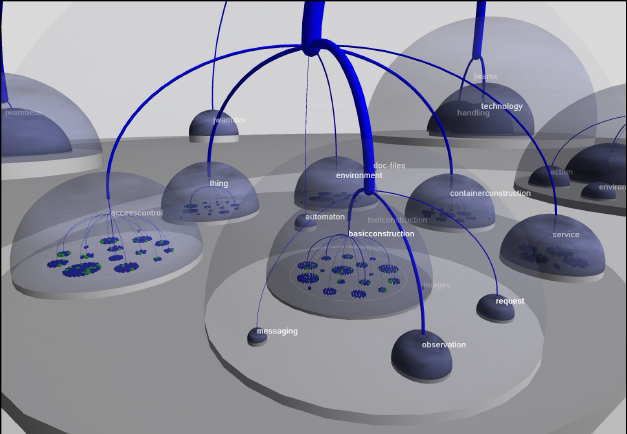
\includegraphics{balzert_tubes.png}}
\caption{Visualisierung von Beziehungen mit gekrümmten 3D-Röhren aus \cite{balzer_hierarchy_2004}}\label{visualisierung:balzert-tubes}\end{figure}


\chapter{Modellanbindung}
\label{modellanbindung:modellanbindung}\label{modellanbindung::doc}\label{modellanbindung:id1}
Innerhalb des Prozessmodellierungswerkzeugs stellt die Modellanbindung (\hyperref[modellanbindung:ipm3d-uebersicht-modellanbindung]{Abbildung  \ref*{modellanbindung:ipm3d-uebersicht-modellanbindung}}) das Bindeglied zwischen einer Benutzerschnittstelle, wie sie von der Editorkomponente \cite{uli} realisiert wird und dem zu manipulierenden Modell dar ({\hyperref[einleitung:anforderungen]{\emph{Anforderungen (e,f)}}} (\autoref*{einleitung:anforderungen})).

Genauer ergeben sich für die Modellanbindung folgende funktionale Anforderungen:
\begin{enumerate}
\item {} 
Erstellen und Löschen von Modellelementen

\item {} 
Bewegen, Rotieren und Skalieren von Modellelementen

\item {} 
Verändern von Prozessmodellattributen

\item {} 
Modifizieren der Visualisierungsparameter von Modellelementen; beispielsweise Farbe oder Schriftart

\item {} 
Erstellen, Laden und Speichern von Prozessmodellen und deren visueller Repräsentation

\end{enumerate}
\begin{figure}[htbp]
\centering
\capstart

\includegraphics[height=9cm]{ipm3d-uebersicht-modellanbindung.eps}
\caption{Die Modellanbindung im Kontext von i\textgreater{}PM3D}\label{modellanbindung:ipm3d-uebersicht-modellanbindung}\end{figure}


\section{Modellkomponente}
\label{modellanbindung:modellkomponente}\label{modellanbindung:id2}
Wie in {\hyperref[verwendet:simulatorx]{\emph{Simulator X}}} (\autoref*{verwendet:simulatorx}) erläutert, bestehen Simulator-X-Anwendungen aus einer Reihe von Komponenten, die jeweils ein wohl definiertes Aufgabengebiet abdecken.
Die \code{ModelComponent} stellt folglich dem System alle Funktionalitäten zur Verfügung, die im Zusammenhang mit der Manipulation von Modellen stehen (\emph{Anforderung (e)}).

So wird der Zugriff auf die Modelle vollständig von der \code{ModelComponent} gekapselt; es gibt für andere Systembestandteile keine Möglichkeit, direkt darauf zuzugreifen.
Abgesehen von der erhöhten Übersichtlichkeit und Wartbarkeit wird dies auch durch die Actor-basierte Architektur und damit nachrichtenbasierte Kommunikation ("`message passing"') von Simulator X vorgegeben.


\subsection{Commands}
\label{modellanbindung:commands}
Die Modellfunktionen werden zum Teil als \code{Commands} bereitgestellt, die über das Kommunikationssystem von {\hyperref[verwendet:simulatorx]{\emph{Simulator X}}} (\autoref*{verwendet:simulatorx}) an die \code{ModelComponent} geschickt werden.
In der momentanen Umsetzung werden diese \code{Commands} ausschließlich durch die Editorkomponente genutzt, die von \cite{uli} beschrieben wird.

Es existieren \code{Commands} für die folgenden Funktionen:
\begin{itemize}
\item {} 
Laden von Metamodellen

\item {} 
Laden, Speichern, Erstellen, Schließen und Löschen von (Usage-)Modellen

\item {} 
Erstellen und Löschen von Knoten und Szenenobjekten

\item {} 
Erstellen einer Kante zwischen zwei Knoten

\end{itemize}

Alle anderen Manipulationsmöglichkeiten — das sind diejenigen, die nur Parameter einzelner Modellelemente betreffen – werden über \code{ModelEntities} bereitgestellt, welche weiter unten in diesem Kapitel {\hyperref[modellanbindung:model-entities]{\emph{}}} (\autoref*{modellanbindung:model-entities}) erläutert werden.


\subsection{Übersicht}
\label{modellanbindung:ubersicht}
Da die Funktionalität der \code{ModelComponent} relativ umfangreich ist, ist diese wiederum in die in  \hyperref[modellanbindung:modelcomponent-classdiag]{Abbbildung  \ref*{modellanbindung:modelcomponent-classdiag}} gezeigten "`Unterkomponenten"' aufgeteilt.
\begin{figure}[htbp]
\centering
\capstart

\includegraphics[width=16cm]{modelcomponent-classdiag.eps}
\caption{Unterkomponenten der \code{ModelComponent} (vereinfacht)}\label{modellanbindung:modelcomponent-classdiag}\end{figure}

Das Trait \code{Component} wird von Simulator X bereitgestellt und muss von allen Komponenten implementiert werden.
Dessen Methoden beziehen sich überwiegend auf den {\hyperref[modellanbindung:lebenszyklus]{\emph{"`Lebenszyklus"'}}} (\autoref*{modellanbindung:lebenszyklus}) von \code{Entities}.
Die Implementierung dieser Methoden erfolgt durch das eingemischte Trait \code{ModelComponentEntityLifecycle}.

Von Trait \code{ModelComponentHandlers} werden die Funktionen bereitgestellt, die eingehende Nachrichten (vor allem \code{Commands}) von anderen Komponenten verarbeiten und diese gegebenenfalls beantworten.
Solche Funktionen werden in Simulator X als "`Handler"' bezeichnet.

Das Laden (mittels "`LMMLight-Parser"') und Speichern ("`ModelToText"') sowie die Verwaltung der geladenen (Meta-)Modelle wird der \code{ModelComponent} durch das Object \code{ModelContext} bereitgestellt.


\section{Modell-Persistenz}
\label{modellanbindung:modell-persistenz}
Das Prozessmodellierungswerkzeug muss in der Lage sein, neue Modelle zu erstellen, diese abzuspeichern und wieder zu laden (\emph{Anforderung (f)}).
Die Modelle werden in der Sprache {\hyperref[modellhierarchie:lmmlight]{\emph{LMMLight}}} (\autoref*{modellhierarchie:lmmlight}) beschrieben, welche in Dateien in einer textuellen Darstellung abgelegt und daraus wieder geladen werden kann.

Für das Laden wird der im Rahmen dieser Arbeit entstandene \textbf{LMMLight-Parser} genutzt, der mit Hilfe der Scala-{\hyperref[verwendet:parser-kombinatoren]{\emph{Parser-Kombinatoren}}} (\autoref*{verwendet:parser-kombinatoren}) implementiert wurde.
Der Parser liefert einen Syntaxbaum der textuellen Eingabe, der aus "`unveränderlichen"' (immutable) Objekten aufgebaut ist.


\subsection{Speicherrepräsentation eines LMMLight-Modells}
\label{modellanbindung:speicherreprasentation-eines-lmmlight-modells}
Um die Modelle in der Anwendung verändern zu können, wird der vom Parser gelieferte Syntaxbaum in eine andere Struktur überführt.
Der so erzeugte Objektgraph ist an die an die EMF \cite{www:emf}-Repräsentation zur Laufzeit angelehnt, wie sie in OMME von XText \cite{www:xtext} erzeugt wird.

Vom Graphen wird der hierarchische Aufbau von LMM, wie in {\hyperref[grundlagen:lmm]{\emph{Linguistic Meta Model}}} (\autoref*{grundlagen:lmm}) gezeigt abgebildet.
Die Elemente von LMM werden durch analog benannte Klassen repräsentiert, die mit dem Buchstaben "`M"' beginnen.

So wird die "`Wurzel"' von einer \code{MModel}-Instanz gebildet, der sich \code{MLevels} unterordnen, die wiederum \code{MPackages} mit \code{MConcepts} sowie weiteren \code{MPackages} enthalten.
Weiterhin kann ein \code{MConcept} andere \code{MConcepts} referenzieren. So ergibt sich ein azyklischer, gerichteter Graph.
Ausgehend von einem \code{MModel}-Objekt kann die \code{ModelComponent} in einem Modell navigieren und es modifizieren, beispielsweise neue Concepts anlegen.

\hyperref[modellanbindung:domain-model-beispiel]{Abbildung  \ref*{modellanbindung:domain-model-beispiel}} zeigt beispielhaft einen Ausschnitt aus der Speicherrepräsentation des {\hyperref[modellhierarchie:domain-model-stack]{\emph{Domain-Model-Stacks}}} (\autoref*{modellhierarchie:domain-model-stack}).
Im Beispiel ist das Concept \code{ProcessUsage} eine Verwendung von \code{ProcessA}.
Mit \code{ProcessUsage} ist daher eine \code{MConceptReference} assoziiert, welche die Spezialisierungsrelation zwischen den beiden Concepts repräsentiert.
\code{ProcessUsage} hat außerdem eine ausgehende Kante zu einer anderen (nicht gezeigten) Verwendung.
Ausgedrückt wird dies durch die Zuweisung vom Typ \code{MConceptAssignment}, welche wiederum die zugehörige Kante \code{ControlFlowA} referenziert.
Die Zuweisung gehört zu einem Attribut mit dem Namen "`outboundControlFlows"', das im Concept \code{Node} aus dem {\hyperref[metamodelle:pmm]{\emph{Prozess-Metamodell}}} (\autoref*{metamodelle:pmm}) definiert ist.
\begin{figure}[htbp]
\centering
\capstart

\includegraphics[width=18cm]{domain-model-beispiel.eps}
\caption{Speicherrepräsentation eines Beispiel-Prozessmodells (Ausschnitt)}\label{modellanbindung:domain-model-beispiel}\end{figure}


\subsection{Vereinfachung des Umgangs mit Modellen}
\label{modellanbindung:vereinfachung-des-umgangs-mit-modellen}
Um den Zugriff auf die Modelle zu vereinfachen und öfter vorkommende Aufgaben auszulagern, wurde eine Reihe von Adaptern für die in der Speicherrepräsentation der Modelle genutzten Klassen implementiert.
Ein Beispiel dafür ist der \code{MConceptAdapter}, dessen Methoden beispielsweise den schnellen Zugriff auf alle zuweisbaren Attribute (\code{assignableAttributes}), das Setzen von Werten (\code{setValue}) oder die Abfrage von Concept-Beziehungen (\code{instanceOf}) erlauben.
Für alle Adapter werden {\hyperref[verwendet:implicit]{\emph{Implizite Methoden}}} (\autoref*{verwendet:implicit}) angeboten, die die gekapselten Objekte direkt um die Methoden "`erweitern"', die in den Adaptern definiert sind.


\subsection{Laden von Metamodellen}
\label{modellanbindung:laden-metamodelle}\label{modellanbindung:laden-von-metamodellen}
Wie in {\hyperref[modellhierarchie:modellhierarchie]{\emph{Modellhierarchie}}} (\autoref*{modellhierarchie:modellhierarchie}) beschrieben wurde, werden Metamodelle für die Spezifikation der verwendeten Modellierungssprache und deren Repräsentation eingesetzt.
Diese sollen prinzipiell austauschbar sein. Dazu wird von der Modellkomponente die Funktion bereitgestellt, Metamodelle zur Laufzeit zu laden.

Um das Laden der Modelle anzustoßen, ist folgendes \code{Command} definiert:

\begin{Verbatim}[commandchars=\\\{\}]
\PYG{k}{case} \PYG{k}{class} \PYG{n+nc}{LoadMetaModels}\PYG{o}{(}\PYG{n}{domainModelPath}\PYG{k}{:} \PYG{k+kt}{String}\PYG{o}{,} \PYG{n}{editorModelPath}\PYG{k}{:} \PYG{k+kt}{String}\PYG{o}{,} \PYG{n}{loadAsResource}\PYG{k}{:} \PYG{k+kt}{Boolean}\PYG{o}{)}
    \PYG{k}{extends} \PYG{n+nc}{Command}
\end{Verbatim}

Von \code{loadAsResource} wird angegeben, ob die Pfade als Java-Resource-Path zu einer Metamodell-Datei interpretiert ("`true"') oder direkt im Dateisystem gesucht werden sollen ("`false"').

Es wird zur Vereinfachung der Implementierung davon ausgegangen, dass die Metamodelle der Domäne und des Editors immer paarweise geladen werden.
Mehrere Repräsentationen zu einer Domäne zu laden ist somit noch nicht möglich.
Die Modellkomponente lässt prinzipiell das Laden von mehreren Metamodell-Paaren zu. Jedoch wird dies von der Editorkomponente \cite{uli} noch nicht unterstützt.

Nachdem die Metamodelle geladen worden sind, werden von der Modellkomponente Informationen aus den Modellen ausgelesen, die für die Editorkomponente relevant sind.
Zum Einen ist dies eine Auflistung der verfügbaren Kanten- und Szenenobjekttypen, die vom Benutzer erzeugt werden können und die der Editor zu diesem Zweck in seiner Palette anzeigt.
Zum Anderen wird der Editor über die Knoten-"`Metatypen"' informiert, von denen nach dem Typ-Verwendungs-Konzept zur Laufzeit Typen vom Benutzer angelegt werden.

Die Kommunikation zwischen Editor- und Modellkomponente wird in \hyperref[modellanbindung:load-metamodels-sequencediag]{Abbildung  \ref*{modellanbindung:load-metamodels-sequencediag}} am Laden von Metamodellen beispielhaft gezeigt.
Nachrichten, die mit Großbuchstaben beginnen stellen \code{Commands} beziehungsweise Replies dar; Nachrichten mit Kleinbuchstaben sind gewöhnliche Methodenaufrufe und -rückgabewerte.
\begin{figure}[htbp]
\centering
\capstart

\includegraphics[width=16cm]{loadMetamodels-sequencediag.eps}
\caption{Sequenzdiagramm LoadMetaModels (vereinfacht).}\label{modellanbindung:load-metamodels-sequencediag}\end{figure}


\subsection{Laden und Schließen von und Umgang mit mehreren Modellen}
\label{modellanbindung:laden-und-schlieszen-von-und-umgang-mit-mehreren-modellen}
Ein konkretes "`Prozesmodell"' wird geöffnet, indem das zugehörige \emph{Domain-Model} und \emph{Editor-Usage-Model} geladen werden.
Zusammen werden diese beiden Modelle im Folgenden vereinfachend das \emph{Usage-Modell} genannt, welches den aktuellen Zustand eines Prozessmodells und dessen Repräsentation im Editor umfasst\footnote{
Die Benennung "`Usage-Model"' ist eigentlich nicht ganz passend, da das {\hyperref[modellhierarchie:domain-model]{\emph{Domain-Model}}} (\autoref*{modellhierarchie:domain-model}) auch die vom Benutzer erstellten Knotentypen umfasst. Da diese Bezeichnungsweise in der Implementierung zu finden ist, wird diese hier ebenfalls genutzt.
}.

Das \code{Command} \code{LoadUsageModels} ist analog zum \code{Command} \code{LoadMetaModels} definiert, wie im vorherigen Unterabschnitt beschrieben.

Es können von der Anwendung zur Laufzeit mehrere Usage-Modelle (zu denselben Metamodellen) geladen werden.
In der \code{ModelComponent} ist jeweils ein Usage-Model-Paar als "`aktiv"' gekennzeichnet.
Commands wie das Erstellen von Knoten beziehen sich immer auf das aktive Usage-Model. Welches Modell "`aktiv"' ist kann über das \code{Command} \code{SetActiveUsageModel} geändert werden.

Modelle können über \code{CloseUsageModel} wieder geschlossen werden, wobei alle seit dem letzten Speichern erfolgten Änderungen verloren gehen.

Der Umgang mit mehreren Modellen wird auch von der Editorkomponente unterstützt.

Nachdem ein Usage-Model geladen wurde, wird der Aufrufer analog zum Laden der Metamodelle über die im \emph{Domain-Model} definierten Knotentypen informiert.


\subsection{Speichern von Modellen}
\label{modellanbindung:speichern-von-modellen}
"`Speichern"' bedeutet hier, dass die Änderungen an Modellelementen in das Usage-Model zurückgeschrieben werden und das dieses anschließend in textueller Form persistiert wird.
Analog zu \code{LoadUsageModels} werden bei \code{SaveUsageModels} zwei Dateinamen für Domain- und Editormodell angegeben. Java-Resource-Pfade sind hier nicht erlaubt.

Um die Speicherrepräsentation des Modells wieder in eine durch den LMMLight-Parser lesbare\footnote{
Die Darstellung ist aber auch durchaus "`menschenlesbar"' und wird ähnlich formatiert wie im Metamodell-Editor von OMME.
}, textuelle Darstellung zu überführen, wird der in {\hyperref[verwendet:stringtemplate]{\emph{StringTemplate}}} (\autoref*{verwendet:stringtemplate}) vorgestellte Wrapper für die StringTemplate-Bibliothek genutzt.


\section{Modell-Entitäten}
\label{modellanbindung:modell-entitaten}\label{modellanbindung:model-entities}
Objekte, mit denen verschiedene Teile des Systems interagieren, werden in {\hyperref[verwendet:simulatorx]{\emph{Simulator X}}} (\autoref*{verwendet:simulatorx}) durch Entities beschrieben.
Es ist daher zweckmäßig, für jedes Modellelement sowie für Szenenobjekte eine zugehörige Entity zu erstellen.
\code{ModelEntities} werden von der \code{ModelComponent} erzeugt, wenn über ein Command die Erstellung von neuen Elementen angefordert oder ein Modell geladen wird.

Wie aus {\hyperref[verwendet:simulatorx]{\emph{Simulator X}}} (\autoref*{verwendet:simulatorx}) bekannt werden Entities mit Hilfe von \code{EntityDescriptions} beschrieben, die aus \code{Aspects} aufgebaut sind.
In \hyperref[modellanbindung:entity-description]{Abbildung  \ref*{modellanbindung:entity-description}} ist ein eine solche \code{Entity}-Definition zu sehen.
Der Ablauf bei der Erstellung einer \code{ModelEntity} aus einer \code{EntityDescription} wird im Abschnitt {\hyperref[modellanbindung:lebenszyklus]{\emph{Übersicht über den Lebenszyklus von Model-Entitäten}}} (\autoref*{modellanbindung:lebenszyklus}) vorgestellt.
\begin{figure}[htbp]
\centering
\capstart

\includegraphics[width=16.5cm]{entity_description.eps}
\caption{\code{EntityDescription} für einen Knoten (nur ausgewählte und vereinfachte Attribute)}\label{modellanbindung:entity-description}\end{figure}


\subsection{Aspekte}
\label{modellanbindung:aspekte}\label{modellanbindung:modelentities-aspects}
Die zur Erstellung von \code{ModelEntities} genutzten \code{Aspects} werden im Folgenden beschrieben.


\subsubsection{Physik}
\label{modellanbindung:physik}
Knoten und Szenenobjekte sollen in die physikalische Simulation eingebunden werden, um Kollisionen zu erkennen und eine Auswahl der Elemente zu ermöglichen \cite{uli} \cite{buchi}.
Hierfür stellt die Physikkomponente verschiedene \code{Aspects} bereit, die besagen, dass eine bestimmte physikalische Repräsentation zu einer Entity erzeugt werden soll.
Da bisher nur annähernd quaderförmige Geometrien für die Visualisierung von Knoten genutzt werden, wird hier für alle Knoten der \code{PhysBox}-Aspect (\hyperref[modellanbindung:entity-description]{Abbildung  \ref*{modellanbindung:entity-description}}) verwendet.

Kanten definieren keinen Physik-Aspect und besitzen daher keine physikalische Repräsentation\footnote{
Dies ist nicht nötig, da die Auswahl von Kanten nicht unterstützt werden soll und Kollisionen mit Verbindungen eher als hinderlich gesehen wurden. Außerdem könnte eine große Anzahl von Verbindungen schnell zu Geschwindigkeitsproblemen der Physiksimulation führen.
}.


\subsubsection{Grafik}
\label{modellanbindung:grafik}
Die {\hyperref[renderkomponente:renderkomponente]{\emph{Renderkomponente}}} (\autoref*{renderkomponente:renderkomponente}) stellt verschiedene \code{RenderAspects} bereit, die der Renderkomponente alle nötigen Informationen mitteilen, um ein Visualisierungsobjekt zur entsprechenden Entity anzulegen.

Szenenobjekte, welche aus COLLADA-3D-Modelldateien geladen werden, werden von der Renderkomponente selbst erzeugt.
Solche Szenenobjekte sind statisch durch das 3D-Modell definiert.
Das bedeutet in diesem Zusammenhang, dass ihr Erscheinungsbild zur Laufzeit nicht geändert werden kann (abgesehen von Position, Rotation und Skalierung).
In der Entity-Beschreibung wird dafür der \code{ShapeFromFile}-Aspect angegeben.

Für Knoten und Kanten wird dagegen der \code{ShapeFromFactory}-Aspect genutzt, der besagt, dass sich die {\hyperref[renderkomponente:renderkomponente]{\emph{Renderkomponente}}} (\autoref*{renderkomponente:renderkomponente}) das Grafikobjekt von einer externen Factory erzeugen lassen soll.
In \hyperref[modellanbindung:entity-description]{Abbildung  \ref*{modellanbindung:entity-description}} ist zu sehen, dass im \code{Aspect} die \code{ModelDrawableFactory} angegeben wird, welche alle Grafikobjekte für Knoten und Kanten erzeugt.
Parameter \code{creationData} gibt den Typ des gewünschten Objekts an, der in den Figuren im {\hyperref[metamodelle:ebl-figures]{\emph{Editor-Metamodell}}} (\autoref*{metamodelle:ebl-figures}) spezifiziert wurde.
Die \code{ModellDrawableFactory} wird später in einem {\hyperref[renderbib:beispiel-neue-modellfigur]{\emph{Anwendungsbeispiel}}} (\autoref*{renderbib:beispiel-neue-modellfigur}) modifiziert, um ein Grafikobjekt für einen neuen Knotentyp hinzuzufügen.


\subsubsection{Modell}
\label{modellanbindung:modell}
Für die drei Elementtypen Knoten, Kanten und Szenenobjekte gibt es jeweils einen Aspect, der von \code{ModelAspect} abgeleitet ist, wie beispielsweise den \code{NodeAspect}, wie er in \hyperref[modellanbindung:entity-description]{Abbildung  \ref*{modellanbindung:entity-description}} zu sehen ist.
\code{ModelAspects} sind der \code{ModelComponent} zugeordnet und enthalten für Nutzer der \code{ModelEntity} relevante Informationen.

Für alle Elemente, die von \code{ModelEntities} repräsentiert werden wird ein vollqualifizierter Name (\code{fqn}) vergeben, der das Element eindeutig innerhalb des Systems identifiziert.
Dieser Name wird in \code{Commands} verwendet, die sich auf bestimmte Elemente beziehen, wie beispielsweise das Verbinden oder Löschen von Knoten.
Bei Knoten und Kanten wird dafür die FQN des entsprechenden Modellelementes aus dem \emph{Domain-Model} genutzt. Szenenobjekte werden über die FQN des \emph{Editor-Usage}-Concepts identifiziert\footnote{
Dass hier die FQNs aus dem Modell genutzt werden hat keine besondere Bedeutung und ist nur ein "`Implementierungsdetail"', auf das man sich nicht verlassen solle.
}.

Außerdem wird ein Identifikationsstring (\code{creatorId}) mitgeliefert, der vom Ersteller eines Elements definiert wird.
Mit "`Ersteller"' ist hier der Absender des entsprechenden \code{Commands} oder die \code{ModelComponent} selbst gemeint.
Diese ID kann von diesem dafür benutzt werden, neu erstellte Entities in internen Datenstrukturen richtig zuzuordnen.


\subsection{Setzen und Auslesen von Position, Ausrichtung und Größe}
\label{modellanbindung:model-svars-transformation}\label{modellanbindung:setzen-und-auslesen-von-position-ausrichtung-und-grosze}
(Dieser Unterabschnitt beschreibt von Simulator X vorgegebene Funktionalität. Projektspezifische Anpassungen sind mit Fußnoten versehen.)

Position und Ausrichtung sind – wie in der Computergrafik üblich \cite{akenine-moller_real-time_2008} – zu einer Transformations-Matrix zusammengefasst.
Die Skalierung eines Objekts wird durch einen Vektor (mit drei Komponenten) angegeben\footnote{
Skalierung wurde für das Projekt hinzugefügt. Dazu wurde die Physikkomponente modifiziert und die selbstgeschriebene Renderkomponente entsprechend ausgelegt.
}.
Beide Werte werden für Knoten und Szenenobjekte von der Physikkomponente verwaltet.

Sie können von anderen Komponenten verändert werden, indem eine Nachricht an die Physikkomponente geschickt wird:

\begin{Verbatim}[commandchars=\\\{\}]
\PYG{n}{physics} \PYG{o}{!} \PYG{n+nc}{SetTransformation}\PYG{o}{(}\PYG{n}{newTransformationMatrix}\PYG{o}{)}
\PYG{n}{physics} \PYG{o}{!} \PYG{n+nc}{SetScale}\PYG{o}{(}\PYG{n}{newScaleVector}\PYG{o}{)}
\end{Verbatim}

Von der Physikkomponente werden außerdem zwei SVars zur Entity hinzugefügt (Typen \code{ScaleVec} und \code{Transformation}), die allerdings nur lesend genutzt werden dürfen.

Beispielsweise kann so die aktuelle Transformation ausgegeben werden\footnote{
Die svarGet-Methode (ebenfalls svarSet und weitere) wurde für das Projekt in einem impliziten Wrapper für Entities definiert um den Zugriff auf SVars zu "`verschönern"'.
}:

\begin{Verbatim}[commandchars=\\\{\}]
\PYG{n}{processEntity}\PYG{o}{.}\PYG{n}{svarGet}\PYG{o}{(}\PYG{n+nc}{Transformation}\PYG{o}{)} \PYG{o}{\PYGZob{}}
    \PYG{n}{value} \PYG{k}{=\textgreater{}} \PYG{n}{println}\PYG{o}{(}\PYG{l+s}{"current transformation of processEntity: "} \PYG{o}{+} \PYG{n}{value}\PYG{o}{)}
\PYG{o}{\PYGZcb{}}
\end{Verbatim}

Dabei ist zu beachten, dass der Get-Aufruf "`nicht-blockierend"' erfolgt.
Wie in {\hyperref[verwendet:simulatorx]{\emph{Simulator X}}} (\autoref*{verwendet:simulatorx}) beschrieben wurde, muss der Wert einer SVar eventuell von einem anderen Actor über das Kommunikationssystem angefragt werden.
Die anonyme Funktion (im Code-Beispiel in geschweiften Klammern) wird ausgeführt, sobald die Antwort vorliegt.

Für Objekte ohne Physik-Aspekt (Kanten) werden die genannten SVars durch die Renderkomponente bereitgestellt.
Diese leisten dasselbe, dürfen aber auch verändert werden:

\begin{Verbatim}[commandchars=\\\{\}]
\PYG{n}{processEntity}\PYG{o}{.}\PYG{n}{svarSet}\PYG{o}{(}\PYG{n+nc}{Transformation}\PYG{o}{)}\PYG{o}{(}\PYG{n}{newTransformationMatrix}\PYG{o}{)}
\end{Verbatim}


\subsection{Modell-SVars}
\label{modellanbindung:modellanbindung-svars}\label{modellanbindung:modell-svars}
Weitere Parameter der Modellobjekte lassen sich ebenfalls über \code{SVars} auslesen und setzen.

Diese \code{SVars} lassen sich in drei Gruppen einteilen.
SVars können direkt Attribute aus den beiden zugrunde liegenden (Meta)-Modellen abbilden oder von der Modellkomponente definiert sein:
\begin{enumerate}
\item {} 
\textbf{Domain-Model-SVars}:
Solche SVars werden zu Attributen erzeugt, die im \emph{Domain-Meta-Model} definiert sind und denen in Concepts im \emph{Domain-Model} Werte zugewiesen werden können.
Sie stellen somit die Schnittstelle dar, über die Modellattribute wie die Funktion eines Prozesses oder der Name eines Konnektors verändert werden können.
Unterstützt werden alle literalen Datentypen; den SVars werden die passenden Scala-Datentypen zugewiesen.

\item {} 
\textbf{Editor-Model-SVars}:
Diese SVars werden nach Bedarf aus den Attributen des \emph{Editor-Metamodels} erstellt.
Sie erlauben es, die Visualisierung der Elemente anzupassen, wie sie im Editormodell beschrieben wird\footnote{
Es wäre auch erlaubt, Attribute zu integrieren, die nicht direkt die Visualisierung betreffen, aber das Editor-Verhalten modifizieren. Dies wird bisher aber nicht genutzt.
}.
Neben literalen Attributen werden hier auch Attribute unterstützt, die Concepts referenzieren. Letztere werden für die meisten hier genannten SVars benötigt.

Welche Editor-Attribute unterstützt werden wird von der \code{ModelComponent} festgelegt; dies sind\footnote{
Es war nicht möglich, die Implementierung (auf einfachem Wege) so flexibel zu gestalten wie bei Domain-Model-SVars, was leider dazu führt, dass man keine Attribute hinzufügen kann ohne die \code{ModelComponent} anzupassen.
}:
\begin{itemize}
\item {} 
Hintergrundfarbe (\code{backgroundColor})

\item {} 
Schrift (\code{font})

\item {} 
Schriftfarbe (\code{fontColor})

\item {} 
Texturpfad (\code{texture})

\item {} 
Liniendicke (\code{thickness})

\item {} 
Spekulare Farbe (\code{specularColor})

\end{itemize}

\item {} 
\textbf{Editor-SVars}:
Dies sind SVars, die keine direkte Entsprechung im Modell haben und deren Werte daher auch nicht persistiert werden.
Sie sind automatisch für alle Modellelemente definiert oder werden durch Modellattribute "`aktiviert"'.
\begin{itemize}
\item {} 
SVars für die Auswahl von {\hyperref[visualisierung:visualisierungsvarianten]{\emph{Visualisierungsvarianten}}} (\autoref*{visualisierung:visualisierungsvarianten}):
\begin{itemize}
\item {} 
Deaktivierung (\code{disabled}),

\item {} 
Hervorhebung (\code{highlighted})

\item {} 
Selektion (\code{selected})

\end{itemize}

\item {} 
Parameter für die Visualisierungsvarianten
\begin{itemize}
\item {} 
Breite des Selektionsrahmens (\code{borderWidth})

\item {} 
Hevorhebungsfaktor (\code{highlightFactor})

\item {} 
Transluzenzfaktor bei deaktivierten Elementen (\code{deactivatedAlpha})

\end{itemize}

\end{itemize}

Alle hier genannten SVars werden von der Modellkomponente aktiviert, wenn im Modell das Attribut \code{interactionAllowed} auf "`true"' gesetzt ist.

\end{enumerate}

Alle SVars müssen eindeutig durch eine \code{SVarDescription} beschrieben werden, der ein Symbol zur Identifizierung und einen Scala-Datentyp umfasst.
Die Symbole für Editor-SVars beginnen mit \code{editor}; Symbole für \emph{Domain-Model}-SVars werden mit \code{model} gekennzeichnet.
Daran wird der Attributname aus dem Modell oder im Falle der \emph{Editor}-SVars einer der unter 3. genannten Bezeichner angehängt, abgetrennt durch einen Punkt.


\subsubsection{Anwendungsbeispiel}
\label{modellanbindung:anwendungsbeispiel}
Die Nutzung erfolgt analog zu den schon gezeigten {\hyperref[modellanbindung:model-svars-transformation]{\emph{SVars}}} (\autoref*{modellanbindung:model-svars-transformation}), wozu ebenfalls ein impliziter Wrapper definiert ist.
Im folgenden Beispiel wird die Funktion eines Prozessknotens und die Schriftfarbe über die zugehörige Entity verändert:

\begin{Verbatim}[commandchars=\\\{\}]
\PYG{n}{processEntity}\PYG{o}{.}\PYG{n}{svarSet}\PYG{o}{(}\PYG{l+s}{"model.function"}\PYG{o}{)}\PYG{o}{(}\PYG{l+s}{"Ausarbeitung schreiben"}\PYG{o}{)}
\PYG{n}{processEntity}\PYG{o}{.}\PYG{n}{svarSet}\PYG{o}{(}\PYG{l+s}{"editor.fontColor"}\PYG{o}{)}\PYG{o}{(}\PYG{n+nc}{Color}\PYG{o}{.}\PYG{n+nc}{BLACK}\PYG{o}{)}
\end{Verbatim}


\section{Übersicht über den Lebenszyklus von Model-Entitäten}
\label{modellanbindung:ubersicht-uber-den-lebenszyklus-von-model-entitaten}\label{modellanbindung:lebenszyklus}
Dieser Abschnitt zeigt kurz, welche wichtigen Schritte im "`Lebenszyklus"' einer \code{ModelEntity} durchlaufen werden.

Komponenten in {\hyperref[verwendet:simulatorx]{\emph{Simulator X}}} (\autoref*{verwendet:simulatorx}) definieren eine Reihe von Methoden, die vom Framework beim Erstellen oder Löschen einer Entity aufgerufen werden.

Die Erstellung einer \code{ModelEntity} folgt dem folgenden Schema:
\begin{enumerate}
\item {} 
Der Vorgang wird beispielsweise durch ein \code{CreateNode-Command} vom Editor angestoßen. Die Modellkomponente erzeugt daraufhin eine \code{EntityDescription} mit den {\hyperref[modellanbindung:modelentities-aspects]{\emph{Aspekten}}} (\autoref*{modellanbindung:modelentities-aspects}) und übergibt diese an das Framework (Methode \code{EntityDescription.realize}), welches die Erstellung der Entity verwaltet und die folgenden Methoden aufruft.

\item {} 
Die Methode \code{getAdditionalProvidings} gibt eine Sequenz von \code{SVarDescriptions} zurück, die zu der Entity hinzugefügt werden sollen. Im Falle der Modellkomponente sind dies \code{SVarDescriptions} zu den im vorherigen Abschnitt beschriebenen SVars.

\item {} 
Anschließend wird die Methode \code{getInitialValues} aufgerufen, welche Initialwerte für die definierten SVars zurückgeben soll. Die Modellkomponente liest hierzu die Attributzuweisungen aus den Modell-Concepts aus oder setzt Standardwerte.

\item {} 
Nach Fertigstellung einer Entity wird \code{newEntityConfigComplete} aufgerufen. Die Modellkomponente fügt die Entity zu ihrer internen Repräsentation hinzu und verbindet die Domain-Model-SVars mit den Attributen im Modell. Dies heißt, dass auf der SVar eine "`Observe"'-Funktion registriert wird, die bei jeder Änderung des SVar-Wertes auch den Wert im dahinterliegenden Domain-Concept ändert.\footnote{
Bei den Editor-Model-SVars wird ein anderer Ansatz genutzt, da diese teilweise häufig geändert werden (vor allem die Position). Diese SVars werden erst beim Speichern des Modells ausgelesen und zurückgeschrieben, um Probleme mit der Ausführungsgeschwindigkeit zu vermeiden.
}

\item {} 
Zum Abschluss werden Observer benachrichtigt, die auf die Erstellung von neuen Entities hören. Dies ist hier konkret die Editorkomponente, die auf diesem Weg die Entity zu ihrer internen Repräsentation hinzufügen kann.

\end{enumerate}

Der genannte Ablauf spielt sich auch parallel für die anderen Komponenten ab, für die Aspects in der Entity definiert sind; hier also für die Render- und gegebenenfalls die Physikkomponente.

Beim Löschen spielt sich Folgendes ab:
\begin{enumerate}
\item {} 
Das Löschen wird beispielsweise durch ein DeleteNode(fqnToDelete)-\code{Command} vom Editor initiiert. Daraufhin startet die Modellkomponente den Löschvorgang, indem auf der zur FQN gehörigen Entity die Methode \code{remove} aufgerufen wird.

\item {} 
Simulator X entfernt nun die Entity aus dem System und ruft dabei in der Komponente die \code{removeFromLocalRep}-Methode auf. In dieser Methode sollen interne Verweise und zugehörige Daten in den Komponenten entfernt werden.

\end{enumerate}
\begin{figure}[htbp]
\centering
\capstart

\includegraphics[width=18cm]{entity-erstellen-aktivitaet.eps}
\caption{Ablauf der Erstellung einer ModelEntity durch die Editorkomponente}\label{modellanbindung:entity-erstellen-aktivitaet}\end{figure}


\chapter{Renderkomponente}
\label{renderkomponente:renderkomponente}\label{renderkomponente::doc}\label{renderkomponente:id1}
In diesem Kapitel wird die Renderkomponente vorgestellt, die die Grafikfunktionen\footnote{
Die Implementierung umfasst auch die Übersetzung von Tastatur- und Mausdaten, die von LWJGL geliefert werden, in Simulator X - Events. Für diese Arbeit sind aber nur die Grafikfunktionen relevant.
} für i\textgreater{}PM3D bereitstellt.
Von dieser Komponente wird die im Rahmen dieser Arbeit entstandene {\hyperref[renderbib:render-bibliothek]{\emph{Render-Bibliothek}}} (\autoref*{renderbib:render-bibliothek}) an Simulator X angebunden.
Dadurch wird die von Simulator X bereitgestellte Komponente für die grafische Darstellung ersetzt, deren Fähigkeiten nicht ausreichten, um die hier vorgestellte Visualisierung auf einfachem Wege zu implementieren.

Die eigentlichen Render-Aufgaben werden an einen Actor (Klasse \code{MMPERenderActor}) delegiert, der von der Renderkomponente (\code{MMPERConnector}) gestartet wird\footnote{
Dieser Aufbau ergibt sich aus der Idee, für die Darstellung der Szene mehrere Bildschirme nutzen zu können, wie es unter Anderem für ein CAVE-System nötig wäre. Dazu könnten der Renderkomponente mehrere RenderActors zugeordnet werden. Dies war vorgesehen, wird jedoch nicht überall in der Implementierung umgesetzt und daher nicht unterstützt.
}.
Nachrichten, die Grafikfunktionen betreffen werden von anderen Komponenten an die Renderkomponente geschickt und an den RenderActor weitergeleitet.


\section{RenderActor}
\label{renderkomponente:renderactor}
Für den RenderActor musste ein eigener Scheduler für Scala-Actors erstellt werden, da der Standard-Scheduler die Actor-Arbeitspakete in beliebig wechselnden Threads ausführen kann.
Dies ist für die Ausführung von OpenGL-Funktionen problematisch. Deswegen wird die Ausführung der Render-Aufgaben auf einen Thread beschränkt.

Der RenderActor definiert zwei Render-Ebenen. Die zuerst gezeichnete Ebene umfasst alle 3D-Objekte wie den Prozessgraphen und Szenenobjekte.
Darüber wird eine Ebene gezeichnet, die 2D-Elemente wie Cursor der Eingabegeräte oder das Eightpen-Menü \cite{buchi} enthält.
Beide Ebenen werden durch jeweils eine {\hyperref[renderbib:renderstage]{\emph{RenderStage}}} (\autoref*{renderbib:renderstage}) gezeichnet.

Es gibt die Möglichkeit, den RenderActor durch Plugins zu erweitern, die an verschiedenen vordefinierten Erweiterungspunkten im Render-Prozess eingreifen können.
Plugins können neue Grafikobjekte erzeugen und zu einer der beiden \code{RenderStages} hinzufügen oder selbst OpenGL-Funktionen ausführen.
Dies wird im Projekt für die Darstellung der Nifty-GUI-Menüs \cite{uli} und des Eightpen-Menüs \cite{buchi} genutzt.


\section{OpenGL-Versionsproblematik}
\label{renderkomponente:opengl-versionsproblematik}
Die Library Nifty-GUI bringt eine eigene Render-Implementierung auf Basis von OpenGL 1.x mit, welche auch Funktionen nutzt, die in OpenGL 3.3 als "`veraltet"' ("`deprecated"') eingestuft sind.
Von der Render-Bibliothek werden dagegen nur Funktionen genutzt, die in OpenGL 3.3 verfügbar sind.

Wegen Nifty-GUI muss die Renderkomponente OpenGL 3.3 im Kompatibilitätsmodus betreiben, der auch die "`deprecated"'-Funktionen unterstützt.
Es ist möglich, dass dies auf manchen Hardwareplattformen zu Geschwindigkeits- oder Darstellungsproblemen führt.


\section{Projektspezifische Erweiterungen}
\label{renderkomponente:projektspezifische-erweiterungen}
Die Renderkomponente unterstützt die von Simulator X bereitgestellten \code{RenderAspects} für die Definition von Lichtquellen-Entities (\code{PointLight}) sowie den Aspect \code{ShapeFromFile}, der die Renderkomponente anweist, die grafische Repräsentation einer Entity aus einer COLLADA-Modelldatei zu laden.

Im Folgenden werden die Funktionalitäten aufgelistet, welche von der ursprünglichen Renderkomponente nicht unterstützt werden.


\subsection{ShapeFromFactory}
\label{renderkomponente:shapefromfactory}
Mir der hier entwickelten Renderkomponente ist es möglich, die grafische Repräsentation einer Entity von einer Factory-Klasse oder -Actor erzeugen zu lassen.
Damit lassen sich in der Anwendung beliebige Grafikobjekte nutzen, die mit Hilfe der {\hyperref[renderbib:render-bibliothek]{\emph{Render-Bibliothek}}} (\autoref*{renderbib:render-bibliothek}) erstellt wurden.

Hierfür ist der RenderAspect \code{ShapeFromFactory} definiert.
Dies wird im Projekt für die Erstellung der Grafikobjekte für Modellelemente – also der Knoten und Kanten des Prozessmodells – genutzt.


\subsection{Modellierungsflächen}
\label{renderkomponente:modellierungsflachen}
Für die Darstellung von {\hyperref[visualisierung:modellierungsflaechen]{\emph{2D-Modellierungsflächen}}} (\autoref*{visualisierung:modellierungsflaechen}) wurde ein \code{PlaneAspect} bereitgestellt, der SVars für die Konfiguration von Transluzenz, Farbe, Linenbreite und -dichte und das Deaktivieren der Linien definiert.


\subsection{2D-Grafikobjekte}
\label{renderkomponente:d-grafikobjekte}
Der Aspect \code{Image2D} wird dafür genutzt, bewegliche und skalierbare 2D-Grafikobjekte darzustellen.
Bei der Erstellung muss ein Pfad zu einer Bilddatei angegeben werden. Position und Größe sind über SVars modifizierbar.
Diese Werte können entweder über die Bildschirm-Pixelkoordinaten oder über normalisierte Koordinaten (von -1 bis +1 in x und y-Richtung) angegeben werden.
Welches Koordinatensystem genutzt wird, wird über den Konstruktor in \code{coordsAreNormalized} angegeben.


\subsection{User-Entity}
\label{renderkomponente:user-entity}
Simulator X stellt eine \code{User}-Entity bereit, über deren SVars \code{HeadTransform} und \code{ViewPlatform} die Position des Benutzers in der 3D-Szene bestimmt wird.
Diese wird von der Renderkomponente erzeugt, die zusätzliche SVars definiert, über die Viewport\footnote{
Größe und Nullpunkt der Zeichenfläche für OpenGL, angegeben in Pixel.
} - (Aspect \code{ViewportSettings}) und Render-Frustum-Einstellungen\footnote{
Diese Einstellungen legen die perspektivische Projektion fest. \cite{www:frustum}
} (Aspect \code{FrustumSettings}) abgefragt werden können\footnote{
Die Werte lassen im Prinzip sich auch verändern, nur wird dies von der Implementierung noch nicht vollständig unterstützt.
}.


\chapter{Render-Bibliothek}
\label{renderbib:render-bibliothek}\label{renderbib::doc}\label{renderbib:id1}
Für die im vorherigen Kapitel beschriebene Renderkomponente wurde eine Anbindung an eine Grafikschnittstelle benötigt, mit der sich die folgenden Anforderungen realisieren lassen:
\begin{enumerate}
\item {} 
Nutzung der Fähigkeiten moderner Grafikhardware, unter Anderem um eine hohe Ausführungsgeschwindigkeit zu erlauben.

\item {} 
Möglichkeit, spezielle Effekte mit Hilfe direkter Programmierung der Grafikhardware flexibel implementieren zu können (Shaderprogrammierung).

\item {} 
Die Grafikausgabe sollte auf verbreiteten Plattformen funktionieren, mindestens auf Windows und Linux.

\item {} 
Bereitstellung von in der Computergrafik üblichen Abstraktionen wie einer Kamera, Lichtquellen und Grafikobjekten, die die Manipulation von Visualisierungsparametern zur Laufzeit erlauben.

\item {} 
Unterstützung von transluzenten Objekten

\item {} 
Darstellung von Schrift und Texturen auf 3D-Objekten, möglichst skalierbar

\item {} 
"`Bild-in-Bild"'-Techniken ("`off-screen rendering"'), also das Zeichnen von 3D-Teil-Szenen in 2D-Bilder, die im Grafikspeicher abgelegt sind und so in eine größere 3D-Szene eingebettet werden können.

\end{enumerate}

Anforderung (5) wird im Projekt für die Darstellung von {\hyperref[visualisierung:deaktivierung]{\emph{deaktivierten Modellelementen}}} (\autoref*{visualisierung:deaktivierung}) sowie {\hyperref[visualisierung:modellierungsflaechen]{\emph{Modellierungsflächen}}} (\autoref*{visualisierung:modellierungsflaechen}) gebraucht.
Anforderung (7) ist auf den Wunsch zurückzuführen, komplexe Menüs wie das Eightpen-Menü \cite{buchi} erstellen zu können, die selbst wieder 3D-Objekte enthalten.

Die Anforderungen (1, 2, 3) werden – auf niedriger Ebene – nur von OpenGL in einer relativ aktuellen Version ab 3.0 erfüllt.
Da "`modernes"' {\hyperref[verwendet:opengl]{\emph{OpenGL}}} (\autoref*{verwendet:opengl}) im Prinzip nur eine direkte Schnittstelle zur Grafikhardware ist, ist die Programmierung wegen fehlender Abstraktion und Wiederverwendbarkeit relativ aufwändig.

Im Gegensatz dazu stehen zahlreiche Frameworks, die verschiedene Aufgabengebiete und Abstraktionsebenen abdecken und auf Low-Level-Schnittstellen wie OpenGL aufsetzen.
Diese könnten die Anforderungen (4–7) selbst abdecken oder zumindest dafür benutzt werden, diese zu implementieren.
Solche Systeme werden oft als "`Game-Engines"' bezeichnet, die in erster Linie für die Erstellung von 3D-Computerspielen gedacht sind, sich aber auch durchaus für andere Visualisierungsaufgaben einsetzen lassen\footnote{
Gezeigt wird dies von \cite{alvergren_3d_2009}; {\hyperref[related:krolovitsch]{\emph{siehe}}} (\autoref*{related:krolovitsch}). Dort sei die C++-Game-Engine Panda3D (über eine Python-Anbindung) genutzt worden, um schnell einen Prototypen für einen 3D-Zustandsdiagramm-Editor zu erstellen.
}.

Für die Java-Plattform sind mit JME3 und Ardor3D zwei relativ aktuelle, in Java implementierte 3D-Frameworks verfügbar.
JME3 lag zu Beginn der vorliegenden Projektes nur in einer Alpha-Version vor und schied deshalb für diese Arbeit aus.
Allgemein ist es bei solchen eher komplexen Frameworks schwer einzuschätzen, ob alle benötigten Grafikeffekte ohne viel Aufwand oder sogar nur mit Änderungen an den Frameworks selbst realisiert werden können.
Insbesondere war dies aufgrund der relativ spärlichen (Wiki-) Dokumentation von Ardor3D der Fall.

Diese Frameworks bieten außerdem eher "`zu viele"' Fähigkeiten an, die über die reine Grafikausgabe hinausgehen, wie beispielsweise eine Physik-Unterstützung oder die Einbindung von Eingabegeräten.
Oft werden verschiedenste Aufgaben wie die Grafikrepräsentation und die räumliche Strukturierung der Szene in einen zentralen "`Szenengraphen"' integriert, mit dem eine Anwendung interagiert.
Dies ist für die vorliegende Anwendung nicht sinnvoll, da sie auf {\hyperref[verwendet:simulatorx]{\emph{Simulator X}}} (\autoref*{verwendet:simulatorx}) basiert, welcher genau diese "`Vermischung"' von Aufgaben verhindern soll und selbst schon eine Komponenten-Infrastruktur für die Realisierung von 3D-Anwendungen bereitstellt.

Für die Integration in Simulator X über die Renderkomponente war deshalb eher eine "`leichtgewichtige"' Lösung wünschenswert, welche nur die Grafikausgabe auf eine einfach benutzbare und erweiterbare Weise realisiert.


\section{Übersicht}
\label{renderbib:ubersicht}
Im Rahmen dieser Arbeit wurde somit eine an die Erfordernisse des Projekts angepasste Render-Bibliothek auf Basis von OpenGL erstellt, die allerdings auch für weitere Projekte verwendet werden kann.
Andere Anwendungen könnten ebenfalls auf Simulator X-Basis mit der neuen {\hyperref[renderkomponente:renderkomponente]{\emph{Renderkomponente}}} (\autoref*{renderkomponente:renderkomponente}) realisiert werden oder die Render-Bibliothek direkt nutzen.

Als Anbindung an OpenGL wird {\hyperref[verwendet:opengl]{\emph{LWJGL}}} (\autoref*{verwendet:opengl}) genutzt.
Es werden nur OpenGL-Funktionen genutzt, die in der Version 3.3 standardmäßig verfügbar sind.
Das heißt, dass auf im OpenGL-Standard "`deprecated"' markierte Funktionalität vollständig verzichtet wurde, welche in Zukunft komplett entfernt werden oder zu Geschwindigkeitsproblemen führen könnte.
Damit ist zu erwarten, dass die Render-Bibliothek auch mit den aktuellsten und zukünftigen OpenGL-Versionen sowie neuer Grafikhardware – zumindest in den nächsten Jahren – kompatibel sein wird.

Die Render-Bibliothek orientiert sich in den Grundkonzepten an der für C++ verfügbaren \emph{Visualization Library} \cite{www:vislib}.
Im Gegensatz zu vielen, umfassenden 3D-Engines sollten dem Benutzer der Bibliothek möglichst wenig Einschränkungen bei der Gestaltung seines Programms auferlegt werden.
Bei der Konzeption der Render-Bibliothek stand die Wiederverwendbarkeit von einzelnen Bestandteilen im Vordergrund, die sich wieder zu höheren Abstraktionen zusammensetzen lassen.

Solche Abstraktionen werden – wenn sie allgemein verwendbar sind – direkt von der Render-Bibliothek angeboten, können aber auch speziell für eine bestimmte Anwendung erstellt werden.
Durch das Prinzip soll der Programmierer von oft wiederkehrenden Aufgaben entlastet werden, aber trotzdem die vollen Möglichkeiten von OpenGL nutzen können, wenn nötig.

Höhere Abstraktionen sollen auch von Programmieren ohne tiefgreifende Computergrafik- und OpenGL-Kenntnisse genutzt werden können.
Ein {\hyperref[renderbib:beispiel-neue-modellfigur]{\emph{Beispiel}}} (\autoref*{renderbib:beispiel-neue-modellfigur}) dafür ist die Möglichkeit, auf einfachem Wege ein neues Grafikobjekt für die Darstellung von Modellelementen zu erstellen.

Die Library lässt sich grob in zwei Schichten, eine \textbf{Low-Level-API} und einer \textbf{Higher-Level-API} aufteilen, die im Folgenden vorgestellt werden.


\section{Low-Level-API}
\label{renderbib:low-level-api}
Das als Grundlage genutzte LWJGL bietet nur eine sehr dünne Abstraktionschicht oberhalb von OpenGL, die vor allem dazu dient, OpenGL-Datentypen auf die Java VM abzubilden und umgekehrt.
Die von LWJGL angebotenen Funktionen entsprechend weitestgehend denen, die durch den OpenGL-Standard vorgegeben und aus Programmiersprachen wie C bekannt sind.

Die Low-Level-API\footnote{
Zu finden im Package mmpe.renderer.gl
} sorgt nun für die objektorientierte Kapselung von OpenGL-Basiselementen und verschiedene Vereinfachungen für Standardfälle.
Diese Schicht ermöglicht es, sehr nahe an den Konzepten von OpenGL zu entwickeln, ohne bei Routineaufgaben selbst viel OpenGL-Code schreiben zu müssen.
Klassen- und Methodennamen orientieren sich, wie bei der Visualization Library, vorwiegend an den gekapselten OpenGL-Funktionen.

Hier soll nur eine kurze Übersicht über die Funktionalitäten gegeben werden, da diese für das Verständnis dieser Arbeit weniger wichtig sind und sehr OpenGL-spezifisch sind.
\begin{description}
\item[{Vertex Buffer Object (VBO)-Klassen für verschiedene Datentypen}] \leavevmode
Vereinfachen die Verwaltung des Grafikspeichers, beispielsweise den Transfer von Daten dorthin.

\item[{Uniform, UniformBlock- und VertexAttribute-Klassen}] \leavevmode
Daten lassen sich so bequem zum Shaderprogramm auf der Grafikkarte übertragen. Die UniformBlock- und VertexAttribute-Klassen bauen auf der VBO-Abstraktion auf.

\end{description}

Beispiel für eine Uniform-Verwendung:

\begin{Verbatim}[commandchars=\\\{\}]
\PYG{k}{val} \PYG{n}{color} \PYG{k}{=} \PYG{n+nc}{ConstVec4}\PYG{o}{(}\PYG{l+m+mi}{1}\PYG{o}{,} \PYG{l+m+mi}{1}\PYG{o}{,} \PYG{l+m+mi}{1}\PYG{o}{,} \PYG{l+m+mi}{1}\PYG{o}{)}
\PYG{k}{val} \PYG{n}{colorUniform} \PYG{k}{=} \PYG{n+nc}{GLUniform4f}\PYG{o}{(}\PYG{l+s}{"color"}\PYG{o}{)}
\PYG{n}{colorUniform}\PYG{o}{.}\PYG{n}{set}\PYG{o}{(}\PYG{n}{color}\PYG{o}{)}
\end{Verbatim}
\begin{description}
\item[{Shader- und ShaderProgram-Klasse}] \leavevmode
Übernehmen das Kompilieren und Linken von Shadern sowie die Verwaltung von Uniforms und UniformBlocks.

\item[{Renderbuffer und Framebuffer-Klassen (FBO)}] \leavevmode
Abstraktionen für das Offscreen-Rendering (Anforderung 5)

\item[{Zeichenbefehle}] \leavevmode
Kapseln die Zeichenfunktionen, welche OpenGL anweisen ein Objekt zu zeichnen. Es werden die Funktionen DrawArrays und DrawElements unterstützt.

\end{description}

Sonstige Abstraktionen: Textur- und Textursampler-Klassen, Viewport und Hintergrundfarbe (glClearColor), OpenGL-Einstellungen (wie glEnable oder glDepthFunc), VertexArrayObjects


\section{Higher-Level-API}
\label{renderbib:higher-level-api}
Diese Schicht stellt im Wesentlichen Schnittstellen und häufig benötigte Implementierungen für die Aufgaben bereit, die grafischen Objekte und den eigentlichen Rendervorgang zu beschreiben, der jene Objekte schließlich "`auf den Bildschirm bringt"'.
Zur Implementierung werden die von der Low-Level-API bereitgestellten OpenGL-Abstraktionen genutzt.

In dieser Bibliothek wird ein solcher Rendervorgang durch sogenannte \textbf{RenderStages} beschrieben.
Objekte, die von solchen RenderStages angezeigt werden können werden als \textbf{Drawable} bezeichnet.


\subsection{Drawable}
\label{renderbib:drawable}\label{renderbib:id4}
Zu zeichnende Objekte werden durch eine Klasse beschrieben, welche von einer Basisklasse \code{Drawable} abgeleitet ist.
Solche Drawable-Klassen müssen eine Beschreibung der Geometrie (Trait \code{Mesh}), der Position und Größe (\code{Transformation}) und der Darstellungsweise (\code{Effect}) enthalten.
Die Implementierung ist dabei sehr flexibel möglich und kann an die Anforderungen des konkret dargestellten Objekts und der Anwendung angepasst werden.

In den Traits sind nur Methoden vorgegeben, welche die von einem "`Renderer"' benötigten Daten liefern müssen:
\begin{itemize}
\item {} 
\code{Mesh} stellt dem Renderer die Zeichenbefehle sowie Vertex-Attribute bereit, üblicherweise sind das Vertexkoordinaten, Normalen und Texturkoordinaten.

\item {} 
\code{Transformation} liefert die Transformationsmatrix des Grafikobjekts.

\item {} 
\code{Effect} ist für die Bereitstellung von Shader-Beschreibungen und zugehörigen Uniforms zuständig.

\end{itemize}

Ein Renderer kann selbst implementiert werden oder es kann eine \code{RenderStage} (nächster Abschnitt) dafür konfiguriert und genutzt werden.

Drawables stellen im Normalfall eine Schnittstelle für die Anwendung bereit, über die sich Attribute des Grafik-Objektes auslesen und setzen lassen.
So könnte eine Transformation, die für ein bewegliches Objekt eingesetzt wird, einen Setter bereitstellen, der das Verändern der aktuellen Position erlaubt.

Die Render-Bibliothek stellt eine Reihe von Implementierungen dieser Traits zur Verfügung.
Diese sind zwar auf die Bedürfnisse des i\textgreater{}PM3D-Projekts abgestimmt, aber möglichst allgemein gehalten und damit wiederverwendbar.

Sinnvollerweise werden Drawables erstellt, indem Traits zusammengemischt werden, die die genannten Basis-Traits \code{Mesh}, \code{Transformation} und \code{Effect} implementieren.
So kann mit diesem Konzept beispielsweise ein Würfel definiert werden, indem eine entsprechende \code{Mesh}-Implementierung erstellt wird.
Durch die Verwendung von unterschiedlichen \code{Effect}-Traits können auf einfachem Wege verschieden dargestellte Varianten eines Objekts erstellt werden.

\hyperref[renderbib:drawable-classdiag]{Abbildung  \ref*{renderbib:drawable-classdiag}} zeigt dieses Drawable-Konzept an einem Beispiel. Es wird nur eine Auswahl der Methoden dargestellt.
\begin{figure}[htbp]
\centering
\capstart

\includegraphics[width=16.5cm]{drawable-classdiag.eps}
\caption{Zusammensetzung eines farbigen Würfels aus den Basis-Traits}\label{renderbib:drawable-classdiag}\end{figure}

Effects selbst können relativ kompliziert aufgebaut sein. Es ist sinnvoll, diese wieder aus verschiedenen Traits zusammenzusetzen, die Teilfunktionalitäten implementieren.
Solche Traits sind in der Render-Bibliothek mit der Endung \code{-Addon} versehen.
Beispielsweise existiert ein \code{PhongLightingAddon} für die Bereitstellung von Lichtparametern und ein \code{TextDisplayAddon}, welches die Anzeige von Schrift auf den Objekten implementiert.

\hyperref[renderbib:effect-classdiag]{Abbildung  \ref*{renderbib:effect-classdiag}} zeigt ein Beispiel für einen \code{Effect}, der aus zwei \code{Addons} zusammengesetzt wird.
Addons stellen oft Uniforms (\code{material-} und \code{lightUniforms} im Beispiel) zur Verfügung, die im Effect kombiniert und von der \code{uniforms}-Methode zurückgegeben werden.
Mittels der Methoden diffuse und specular kann die Anwendung die Reflexionseigenschaften eines Objekts verändern.
\begin{figure}[htbp]
\centering
\capstart

\includegraphics[width=16.5cm]{effect-classdiag.eps}
\caption{Zusammengesetzter PhongMaterialEffect}\label{renderbib:effect-classdiag}\end{figure}

Ressourcen, die potenziell von vielen verschiedenen Drawables geteilt werden können werden im Drawable nur durch eine abstrakte Beschreibung dargestellt.
Texturen werden über eine \code{TextureDefinition} beschrieben; Shaderquelldateien über eine \code{ShaderDefinition}.


\subsection{RenderStage}
\label{renderbib:renderstage}\label{renderbib:id5}
\code{RenderStages} sind für das Zeichnen der grafischen Objekte zuständig. Die Anwendung übergibt einer \code{RenderStage} einmal pro Frame\footnote{
Wie in "`Frames Per Second"' (FPS). Damit ist ein "`Einzelbild"' gemeint.
} alle zu zeichnenden \code{Drawables}.
Diese werden in der bereitgestellten Implementierung der RenderStage zuerst sortiert und anschließend gezeichnet.
Eine Sortierung wird durchgeführt, um transluzente Objekte (Anforderung 7) in der richtigen Reihenfolge zu zeichnen sowie um unnötige Zeichenoperationen und OpenGL-Zustandswechsel zu vermeiden.
Durch Angabe einer Render-Priorität in den Drawables kann manuell eine bestimmte Reihenfolge erzwungen werden, wenn dies für spezielle Zeichenaufgaben nötig ist.

Von der \code{RenderStage} werden zu den von Drawables definierten Texture- und ShaderDefinitions Objekte der Low-Level-API nach Bedarf erzeugt.
Diese werden für das Zeichnen von mehreren Drawables wiederverwendet, um Grafikspeicher und Zeit zu sparen.

Abgegrenzte Funktionalitäten können in ein \code{RenderStagePlugin} ausgelagert werden.
So stellt die Render-Bibliothek unter anderem Plugins für die Verwaltung von Texturen und die Umsetzung von Lichtquellen bereit.

\hyperref[renderbib:renderstage-classdiag]{Abbildung  \ref*{renderbib:renderstage-classdiag}} zeigt eine zusammengesetzte \code{RenderStage}.
\begin{figure}[htbp]
\centering
\capstart

\includegraphics[width=16cm]{renderstage-classdiag.eps}
\caption{RenderStage mit eingemischten Plugin-Traits}\label{renderbib:renderstage-classdiag}\end{figure}


\subsection{Weitere Abstraktionen}
\label{renderbib:weitere-abstraktionen}

\subsubsection{Licht}
\label{renderbib:licht}
Die Render-Bibliothek unterstützt das Phong-Beleuchtungsmodell, welches pixelgenau ausgewertet wird.
Für die Anwendung werden Klassen bereitgestellt, die die von "`altem"' OpenGL bekannten "`Lichtquellen"' bereitstellen und sich an deren Schnittstelle orientieren.
Lichtquellen können entweder entfernungsabhängig (\code{PositionalLight}) oder -unabhängig sein (\code{DirectionalLight}).

Implementiert wird die Beleuchtung auf Scala-Seite durch das Zusammenspiel des \code{PhongLightingRenderStagePlugins} mit dem Effect-Addon \code{PhongLightingAddon}.
Die eigentlichen Lichtberechnungen wurden in GLSL-Shaderfunktionen implementiert, die von verschiedenen Fragment-Shadern genutzt werden können.


\subsubsection{Kamera}
\label{renderbib:kamera}
Die Klasse \code{Camera} repräsentiert eine bewegliche und rotierbare Kamera, die einer \code{RenderStage} zugewiesen werden kann und damit die Perspektive des Betrachters festlegt.
Es werden die von OpenGL bekannten Funktionen (als Methoden von \code{Camera}) angeboten, die eine perspektivische (\code{glFrustum}, \code{gluPerspective}, \code{gluLookAt}) oder orthogonale Projektion (\code{glOrtho}) konfigurieren.
Außerdem stellt die Klasse verschiedene Methoden bereit, die für Umrechnungen von Bildschirm- in 3D-Raumkoordinaten und umgekehrt genutzt werden können (analog zu den OpenGL-Funktionen \code{glProject} und \code{gluUnProject}).

Diese werden im Projekt von Eingabegeräten genutzt, die mit 2D-Daten arbeiten und diese beispielsweise für die Auswahl von 3D-Objekten entsprechend umrechnen müssen.
Aufgrund der von Simulator X geforderten Komponentenaufteilung werden die Methoden von den Nutzern nicht direkt aufgerufen, sondern von der {\hyperref[renderkomponente:renderkomponente]{\emph{Renderkomponente}}} (\autoref*{renderkomponente:renderkomponente}) gekapselt.
Nutzer müssen analog zu den Methoden definierte Nachrichten verwenden, die über das Kommunikationssystem von Simulator X verschickt werden.


\section{COLLADA2Scala-Compiler}
\label{renderbib:collada2scala-compiler}
Das Laden von Modellen direkt aus COLLADA-XML-Dateien ist relativ zeitaufwändig.
Außerdem unterstützt der genutzte COLLADA-Loader \cite{uli} bisher noch nicht die Wiederverwendung der geladenen Modelldaten.
So wird für jede Instanz eines solchen 3D-Modells zusätzlicher Grafikspeicher belegt.
Ein weiteres Problem ist, dass der Loader "`fertige"' \code{Drawables} liefert, die nicht für die Darstellung von Modellelementen (Knoten und Kanten) genutzt werden können.

Aufgrund dessen wurde ein "`Compiler"' entwickelt, der mit Hilfe des COLLADA-Loaders ein Modell lädt und daraus eine Repräsentation der in dem Modell definierten Geometrie in Scala-Code erzeugt.
Die so erzeugte Scala-Quelldatei enthält ein Trait, das {\hyperref[renderbib:drawable]{\emph{Mesh}}} (\autoref*{renderbib:drawable})) implementiert.

Optional kann direkt eine .jar-Datei erstellt werden.

Am Ende des Kapitels wird im Anwendungsbeispiel die Nutzung des COLLADA2Scala-Compilers demonstriert.


\section{Spezielle Erweiterungen für i\textgreater{}PM3D}
\label{renderbib:spezielle-erweiterungen-fur-i-pm3d}
In diesem Abschnitt werden abschließend die Erweiterungen vorgestellt, die speziell für die Realisierung der Prozessvisualisierung bereitgestellt werden ({\hyperref[einleitung:anforderungen]{\emph{Anforderung (f)}}} (\autoref*{einleitung:anforderungen})).
Hier wird auch gezeigt, wie die oben beschriebenen Ebenen der Render-Bibliothek und die GLSL-Shader zusammenwirken.
Außerdem soll verdeutlicht werden, wie {\hyperref[renderbib:drawable]{\emph{Drawables}}} (\autoref*{renderbib:drawable}) als Schnittstelle zwischen grafischer Darstellung und Anwendung dienen.


\subsection{Unterstützung für deaktivierte, hevorgehobene und selektierte Elemente}
\label{renderbib:erweiterung-interaction}\label{renderbib:unterstutzung-fur-deaktivierte-hevorgehobene-und-selektierte-elemente}
Für die {\hyperref[visualisierung:visualisierungsvarianten]{\emph{Visualisierungsvarianten für interaktive Modelleditoren}}} (\autoref*{visualisierung:visualisierungsvarianten}) wurde eine Fragment-Shaderfunktion erstellt, welche die Farbe eines Objektes abhängig von den aktivierten Visualisierungsvarianten verändern kann.
Ein Shader, der diese Funktion nutzt, definiert Uniforms, mit welchen die Varianten ausgewählt werden können.

Auf Scala-Seite werden diese Uniforms vom \code{SelectionHighlightAddon} verwaltet, welches auch eine Schnittstelle für die Anwendung bereitstellt.

Die Varianten lassen sich über im Addon definierte Setter aktivieren:

\begin{Verbatim}[commandchars=\\\{\}]
\PYG{n}{drawable}\PYG{o}{.}\PYG{n}{disabled} \PYG{k}{=} \PYG{k+kc}{false}
\PYG{n}{drawable}\PYG{o}{.}\PYG{n}{highlighted} \PYG{k}{=} \PYG{k+kc}{false}
\PYG{n}{drawable}\PYG{o}{.}\PYG{n}{selectionState} \PYG{k}{=} \PYG{n+nc}{DrawableSelectionState}\PYG{o}{.}\PYG{n+nc}{Selected}
\end{Verbatim}

Durch den Aufruf eines solchen Setters wird die zugehörige Uniform geändert und die Änderung somit zum Shaderprogramm weitergegeben, nachdem etwaige Konvertierungen durchgeführt wurden.

Zusätzlich können noch folgende Parameter gesetzt werden:
\begin{itemize}
\item {} 
\code{borderWidth}: Breite des Selektionsrahmens.

\item {} 
\code{highlightFactor}: Wert, mit dem die berechnete Farbe multipliziert wird um Hervorhebung darzustellen. Bei dunklen Grundfarben wird stattdessen mit 1 / \code{highlightFactor} multipliziert.

\end{itemize}

"`Deaktiviert"' wird durch einen Grauton dargestellt, der wie folgt aus den Komponenten der Grundfarbe berechnet wird: \code{grauwert = (rot + blau + grün) * 0.2}.

Außerdem wird das Objekt transluzent gezeichnet.
Der Selektionsrahmen wird im deaktivierten Zustand abhängig von der resultierenden Helligkeit von "`grauwert"' entweder hellgrau oder dunkelgrau dargestellt.

Die Shaderfunktion zeichnet den "`Selektionsrahmen"' abhängig von den (2D)-Texturkoordinaten, die üblicherweise von 0 bis 1 reichen.
Auf jeder Seite wird ein Bereich mit der Breite "`borderWidth"' als Rahmen in der Komplementärfarbe zum Hintergrund gezeichnet.

So wird durch die Texturkoordinaten die Form des Rahmens definiert; für die in der Arbeit verwendeten Objekte war dies ausreichend.
Jedoch könnten sich bei anderen Figuren Probleme ergeben, da die Texturkoordinaten auch für die Ausrichtung der Textur oder der Schrift genutzt werden.
Für solche Objekte könnte allerdings leicht ein zusätzliches Vertex-Attribut definiert werden, welches die Koordinaten für die Positionierung des Rahmens liefert.\footnote{
Dies ist auch ein Beispiel, dass die Flexibilität von modernem OpenGL (und der Render-Bibliothek) zeigt, die im Gegensatz zu alten OpenGL-Versionen beliebige Vertex-Attribute unterstützen.
}


\subsection{Darstellung von Text}
\label{renderbib:schrift-rendering}\label{renderbib:darstellung-von-text}
Für die Beschriftung von Modellknoten wurde eine gut lesbare und trotzdem einfach umsetzbare Technik für das Rendering von Schrift benötigt.
Hierfür wurde die 2D-API (\code{java.awt}) der Java-Klassenbibliothek zur Hilfe genommen.
Zur Verwendung mit OpenGL wird die Schrift in eine Textur geschrieben, die dann auf die Objekte aufgebracht werden kann.
Um die Darstellungsqualität zu erhöhen, wird die Antialiasing-Funktion von Graphics2D genutzt.

Zur Darstellung von Text müssen Drawables den Trait \code{TextDisplayAddon} einmischen und die genutzte \code{RenderStage} muss die Plugins \code{TextDisplayRenderStagePlugin} sowie \code{TextureRenderStagePlugin} einbinden.
Im RenderStagePlugin wird bei jeder Änderung des Textes oder Schrifteinstellungen die Schrift-Textur neu erstellt, so dass im nächsten Frame der neue Text angezeigt wird.

Der Text kann im Drawable mit

\begin{Verbatim}[commandchars=\\\{\}]
\PYG{n}{drawable}\PYG{o}{.}\PYG{n}{text} \PYG{k}{=} \PYG{l+s}{"irgendein Text"}
\end{Verbatim}

verändert werden. Außerdem werden Einstellmöglichkeiten für die Schriftart, -größe und -stil (\code{java.awt.Font}) und die Schriftfarbe (\code{java.awt.Color}) angeboten.

Der Text wird zentriert angezeigt und am Wortende umgebrochen, falls der horizontale Platz nicht ausreicht.
Die "`Schriftgröße"' wird als Mindestgröße interpretiert; falls ein Objekt eine Skalierung größer eins aufweist, wird die Größe der Schrift proportional mitskaliert.
Bei einer Skalierung kleiner eins wird der für die Schrift zur Verfügung stehende Platz verkleinert.

Die Skalieroperationen werden von einer Shaderfunktion realisiert.

Um auch bei größeren Entferungen von der Kamera und kleiner Schrift noch eine angemessene Lesbarkeit zu erreichen kann Mipmapping genutzt werden, das auch von der Render-Bibliothek unterstützt wird.
Aufgrund von Problemen mit verschiedenen Grafikkarten, die für das Projekt getestet wurden, ist dies standardmäßig jedoch nicht aktiviert.


\subsection{SVarSupport - Einbindung der Modell-Drawables in i\textgreater{}PM3D}
\label{renderbib:svarsupport-einbindung-der-modell-drawables-in-i-pm3d}
Visualisierungsparameter der Modellelemente werden über die \code{ModelComponent} bereitgestellte {\hyperref[modellanbindung:modellanbindung-svars]{\emph{SVars}}} (\autoref*{modellanbindung:modellanbindung-svars}) gesetzt.
Den SVar-Wert zu verändern hat alleine noch keinen Effekt; die Wertänderungen müssen an die Drawables weitergeleitet werden, welche die Anbindung an die Grafikschnittstelle realisieren.

Die Verbindung der SVars mit den Attributen der Drawables erfolgt über Traits, die das Trait \code{SVarSupport} implementieren.
Solche \code{SVarSupports} werden in Modell-Drawables eingemischt, wie im Anwendungsbeispiel im folgenden Abschnitt gezeigt wird.

Diese Traits stellen eine Methode, \code{connectSVars} bereit, die von der Renderkomponente aufgerufen wird nachdem diese ein Drawable erzeugt hat.
So werden in dieser Methode für alle vom Trait unterstützten SVars \emph{Observe-Handler} registriert, die bei jeder Änderung des SVar-Wertes aufgerufen werden.
Üblicherweise leiten diese Funktionen die neuen Werte an Setter des Drawables weiter, wie sie in den vorherigen Abschnitten gezeigt wurden.

Für SVars, deren Typ erst zur Laufzeit bekannt ist, kann der Methode eine "`Ersetzungsliste"' übergeben werden.
Eine solche Ersetzung ist beispielsweise für die Darstellung von Text auf Modellknoten nötig.
Im {\hyperref[metamodelle:ebl-figures]{\emph{Editor-Metamodell}}} (\autoref*{metamodelle:ebl-figures}) wird festgelegt, welches \emph{Domain}-Attribut als Text dargestellt werden soll.
Die Modellkomponente liest den Namen des Attributs aus und definiert eine Ersetzung der \code{Text}-SVar durch die entsprechend benannte {\hyperref[modellanbindung:modellanbindung-svars]{\emph{Domain-Model-SVar}}} (\autoref*{modellanbindung:modellanbindung-svars}).
Beispielsweise wird für einen Prozessknoten die \code{Text}-SVar durch die \code{model.function}-SVar ersetzt.
Für letztere SVar wird so ein \emph{Observe-Handler} registriert, der dem Setter für den aktuellen Text des Drawables jede Änderung an \code{model.function} weitergibt.
Aufgrund dessen wird bei jeder Änderung an dieser SVar (bspw. durch eine Eingabe in einem Menü) der sichtbare Text auf dem Grafikobjekt angepasst.

Das gleiche Prinzip wird für Visualisierungsparameter (bspw. Farben oder die Schriftart) aus dem Editor-Modell angewendet.
\hyperref[renderbib:farbe-setzen-aktivitaet]{Abbildung  \ref*{renderbib:farbe-setzen-aktivitaet}} zeigt beispielhaft, wie sich eine Änderung an der Hintergrundfarbe eines Prozessknotens Benutzer auswirkt und welche Schritte vom Editor-Menü bis zur Grafikkarte durchlaufen werden.


\subsubsection{Beispiele für SVarSupports}
\label{renderbib:beispiele-fur-svarsupports}
Für die im vorherigen Unterabschnitt beschriebene Textdarstellung wird das Trait \code{TextDisplaySVarSupport} angeboten.
Im Normalfall wird dieses zusammen mit dem \code{BackgroundSVarSupport} genutzt, welches das Setzen der Hintergrundfarbe übernimmt.
Das Trait \code{SelectionHighlightSVarSupport} stellt die Anbindung der {\hyperref[renderbib:erweiterung-interaction]{\emph{Visualisierungsvarianten}}} (\autoref*{renderbib:erweiterung-interaction}) bereit.
\begin{figure}[htbp]
\centering
\capstart

\includegraphics[width=17cm]{farbe-setzen-aktivitaet.eps}
\caption{Ablauf bei Änderung der Hintergrundfarbe eines Prozesses durch den Benutzer}\label{renderbib:farbe-setzen-aktivitaet}\end{figure}
\pagebreak

\section{Anwendungsbeispiel: Erstellen von neuen Modell-Figuren}
\label{renderbib:beispiel-neue-modellfigur}\label{renderbib:anwendungsbeispiel-erstellen-von-neuen-modell-figuren}
Zum Abschluss wird gezeigt, wie sich ein neues Grafikobjekt erstellen lässt, das für die Visualisierung eines Knotens eingesetzt werden soll.
Dies ist die Fortsetzung des {\hyperref[metamodelle:beispiel-neues-element]{\emph{Anwendungsbeispiels}}} (\autoref*{metamodelle:beispiel-neues-element}) für das Hinzufügen eines neuen Modellelements zum Metamodell.

Die Geometrie des Objekts kann zum Einen manuell erstellt werden, indem das Trait \code{Mesh} implementiert wird.
Als Vorlage kann eines der mitgelieferten Meshes, wie \code{mmpe.renderer.mesh.UnitCube} genutzt werden.

Einfacher ist die Nutzung des COLLADA2Scala-Compilers, der wie folgt aufgerufen werden kann (Linux):

\begin{Verbatim}[commandchars=\\\{\}]
\PYG{n+nv}{\PYGZdl{} }collada2scala pyramid.dae test.Pyramid pyramid.jar
\end{Verbatim}

Damit wird aus einer COLLADA-Datei pyramid.dae eine pyramid.jar erstellt, die im Package test einen Mesh \code{Pyramid} enthält.

Im nächsten Schritt wird die neue Figur zum object \code{mmpe.model.BaseDrawables} hinzugefügt.

Es soll eine Pyramide erstellt werden, auf deren Seiten Text angezeigt werden kann.
Dafür kann beispielsweise die \code{TextBox} als Vorlage genommen und wie folgt abgeändert werden:

\begin{Verbatim}[commandchars=\\\{\},numbers=left,firstnumber=1,stepnumber=1]
\PYG{k}{class} \PYG{n+nc}{TextPyramid} \PYG{k}{extends} \PYG{n+nc}{EmptyDrawable}\PYG{o}{(}\PYG{l+s}{"textPyramid"}\PYG{o}{)}
  \PYG{k}{with} \PYG{n+nc}{Pyramid}
  \PYG{k}{with} \PYG{n+nc}{SiXTransformation}
  \PYG{k}{with} \PYG{n+nc}{SelectableAndTextEffect}
  \PYG{k}{with} \PYG{n+nc}{SelectionHighlightSVarSupport}
  \PYG{k}{with} \PYG{n+nc}{TextDisplaySVarSupport}
  \PYG{k}{with} \PYG{n+nc}{BackgroundSVarSupport}
\end{Verbatim}

Geändert wurde nur die \code{Mesh}-Implementierung in der 2. Zeile sowie der Name des Objekts in der 1. Zeile.

Abschließend wird in \code{mmpe.model.ModelDrawableFactory} zur Fallunterscheidung in der Methode createDrawables ("`figureFqn match ..."') ein weiterer Fall hinzugefügt:

\begin{Verbatim}[commandchars=\\\{\}]
\PYG{k}{case} \PYG{l+s}{"test.TextPyramid"} \PYG{k}{=\textgreater{}}
  \PYG{k}{val} \PYG{n}{drawable} \PYG{k}{=} \PYG{k}{new} \PYG{n+nc}{TextPyramid}
  \PYG{n+nc}{Seq}\PYG{o}{(}\PYG{n}{drawable}\PYG{o}{)}
\end{Verbatim}

Nun kann die texturierte Pyramide im Editor-Metamodell genutzt werden.
Das hier angegebene "`test.TextPyramid"' entspricht dem \code{scalaType}, wie er im Metamodell gesetzt muss werden muss um diese Figur zu referenzieren.


\subsection{Anmerkungen}
\label{renderbib:anmerkungen}
Am ersten Code-Beispiel ist zu sehen, wie ein Drawable für ein Modellelement prinzipiell definiert wird.
Die Zeilen 2 bis 4 geben die von {\hyperref[renderbib:drawable]{\emph{Drawable}}} (\autoref*{renderbib:drawable}) geforderte Implementierung an.
Es wird von der Renderkomponente vorausgesetzt, dass \code{SiXTransformation} für alle 3D-Drawables genutzt wird.
\code{SelectableAndTextureEffect} wird für alle texturierten Figuren genutzt, die die {\hyperref[renderbib:erweiterung-interaction]{\emph{Visualisierungsvarianten}}} (\autoref*{renderbib:erweiterung-interaction}) unterstützen.
Analog dazu ist \code{SelectableAndTextEffect} für die Textdarstellung definiert, welcher das {\hyperref[renderbib:schrift-rendering]{\emph{TextDisplayAddon}}} (\autoref*{renderbib:schrift-rendering}) nutzt.

In den letzten drei Zeilen werden die \code{SVarSupports} eingemischt, welche die Verbindung zur Anwendung herstellen.


\chapter{Fazit und Ausblick}
\label{schluss::doc}\label{schluss:fazit-und-ausblick}
In der vorliegenden Arbeit wurde die Einbindung von Prozessmodellen und deren Visualisierung im i\textgreater{}PM3D-Prototypen sowie die Spezifikation der verwendeten Modellierungssprache durch Metamodelle vorgestellt.
Aufgrund der Komplexität dieses Themas, der dabei auftretenden Fragestellungen und der insgesamt noch eher schwach ausgeprägten Forschungslage zum Thema 3D-Visualisierung von Prozessen kann dies jedoch nur ein Anfang sein.
In Zukunft wäre es wichtig, die Effizienz von 3D-Visualisierungsansätzen genauer zu untersuchen, wofür der Prototyp eine Grundlage bietet.
Dabei sollten auch Benutzer eingebunden werden, die sich zwar mit dem Thema Prozessmodellierung auskennen, jedoch noch kaum Erfahrung im Umgang mit 3D-Umgebungen haben.

Eingabe und Benutzerinteraktion wurden in dieser Arbeit größtenteils ausgeklammert, da diese von \cite{uli} und \cite{buchi} im Rahmen des Projekts bearbeitet wurden.
Dies ist aber eigentlich ein "`untrennbarer"' Bestandteil, wenn man die Effizienz von 3D-Visualisierungen – insbesondere in interaktiven Modellierungswerkzeugen – bewerten will.
Bei eigenen Versuchen mit dem Prototypen hat sich besonders gezeigt, dass die Effizienz mit dem Vorhandensein gut funktionierender und intuitiver Eingabemethoden steht und fällt.
Daher ist es besonders lohnenswert, zukünftige Arbeiten in diese Richtung zu lenken.

Probleme und naheliegende Erweiterungsmöglichkeiten, welche speziell die Visualisierung betreffen, wurden schon {\hyperref[visualisierung:vis-umsetzung]{\emph{in}}} (\autoref*{visualisierung:vis-umsetzung}) {\hyperref[visualisierung:vis-entwicklungsmoeglichkeiten]{\emph{und}}} (\autoref*{visualisierung:vis-entwicklungsmoeglichkeiten}) besprochen.
Besonders wichtig wären in diesem Zusammenhang umfangreichere Konfigurationsmöglichkeiten, die nach Möglichkeit auch in das Metamodell aufgenommen werden sollten, um eine einheitliche Konfiguration der Visualisierungsparameter zu ermöglichen.
Außerdem sollten in einer Weiterentwicklung automatische Verfahren zur Unterstützung des Benutzers, beispielsweise Layout-Algorithmen und eine intelligente Wahl der Lichtparameter integriert werden.
Daneben kann untersucht werden, inwieweit sich geometriebasierte Ansätze, wia bspw. aus i\textgreater{}PM:sup:\emph{2} bekannt, in den dreidimensionalen Raum übertragen lassen.

Einige bei der Vorstellung von verwandten Arbeiten zur Visualisierung gezeigte Nutzungsmöglichkeiten der dritten Dimension können mit dem Prototypen schon realisiert werden.
Vielversprechend ist die Einbettung der abstrakten Prozessmodelle in eine {\hyperref[related:informations-integration]{\emph{virtuelle Umgebung}}} (\autoref*{related:informations-integration}) mit Abbildern realer Objekte, wie es mit i\textgreater{}PM3D prinzipiell schon möglich ist, da beliebige 3D-Objekte in die Szene eingebunden werden können.
Elemente nach ihrer "`Wichtigkeit"' oder nach anderen Kriterien in unterschiedlicher Entfernung zu zeigen, ist aufgrund der freien Platzierbarkeit der Elemente umsetzbar, verursacht allerdings viel Aufwand für den Benutzer.
Hierfür wäre eine algorithmische Unterstützung vonnöten, die beispielsweise anhand von Attributwerten aus dem Prozessmodell Elemente in einer bestimmten Weise anordnet.

Im Prototypen lassen sich gleichzeitig mehrere Modelle darstellen.
So ist es prinzipiell möglich, hierarchische Modelle mit mehreren Verfeinerungsstufen darzustellen, wie es für die Darstellung von kompositen Prozessen benötigt wird.
Jede Stufe kann so durch ein Modell repräsentiert werden, dessen Modellelemente sich nach Bedarf auf einer {\hyperref[visualisierung:modellierungsflaechen]{\emph{Modellierungsfläche}}} (\autoref*{visualisierung:modellierungsflaechen}) anordnen lassen.

Es fehlt allerdings noch entsprechende Unterstützung, um Beziehungen zwischen mehreren Modellen darzustellen und abzuspeichern.
Verschiedene Modelltypen anzeigen und verknüpfen zu können, ist eine weitere lohnende Entwicklungsmöglichkeit.
Dazu müsste die gleichzeitige Verwendung von mehreren Metamodellen durch die Editorkomponente unterstützt werden ({\hyperref[modellanbindung:laden-metamodelle]{\emph{siehe}}} (\autoref*{modellanbindung:laden-metamodelle})).

Da am Lehrstuhl, an dem dieses Projekt entstanden ist, ebenfalls die umfangreiche Metamodellierungsumgebung OMME entwickelt wird, wäre eine Integration von i\textgreater{}PM3D in diese überlegenswert.
Für die Realisierung des Prototypen wurden schon Prinzipien aus OMME wie die Austauschbarkeit und Separation der Metamodelle für Editor und Modellierungsdomäne sowie die Spezialisierung von Instanzen genutzt.
Um die Flexibilität weiter zu erhöhen und die Anwendbarkeit für verschiedene Modellierungsdomänen zu vereinfachen, sollte nach dem Vorbild von MDF die Spezifikation der grafischen Repräsentation vom Editor-Modell getrennt werden.

Vielversprechend könnten auch Kombinationen von 3D und 2D-Visualisierungen sein, um die Vorteile aus beiden "`Welten"' nutzen zu können.
Dies könnte durch die Integration von 2D-Elementen in i\textgreater{}PM3D realisiert werden.
Außerdem wäre es technisch möglich, i\textgreater{}PM3D auf Basis von \emph{Simulator X} in die Eclipse-Plattform zu integrieren.
Damit könnten 3D-Editoren neben mit MDF spezifizierten 2D-Editoren in derselben Umgebung genutzt werden.

Der Anpassbarkeit der Visualisierung und der Modellierungskonstrukte, die durch die Verwendung des Metamodellierungs-Ansatzes entsteht, muss auch eine entsprechende Flexibilität der Implementierung gegenüberstehen.
In der Modellanbindung wurde diese noch nicht ganz erreicht, da durch diese bisher eine feste Auswahl an Visualisierungsparametern vorgegeben wird, um die Implementierung zu erleichtern.
Dies könnte – möglicherweise auch mit Änderungen in künftigen Versionen von \emph{Simulator X} – wohl flexibler realisiert werden.
\emph{Simulator X} war aber grundsätzlich für die Realisierung des Projekts gut geeignet; besonders die Entkoppelung von Funktionalitäten durch die Komponentenaufteilung und das \emph{Entity / SVar}-Konzept, welche für die Bereitstellung der Modellfunktionalitäten genutzt wurden haben sich als positiv herausgestellt.
Weitere Funktionalitäten zu integrieren, wie beispielsweise die Simulation von Prozessen, visualiert durch die Anzeige von Prozessdaten in der 3D-Szene und durch Animationen von prozessrelevanten Entitäten (bspw. Personen oder Werkstücke) ist durch die Einbindung von zusätzlichen Komponenten leicht möglich. Weiterhin lässt sich auf diesem Wege eine beliebige Erweiterungsmöglichkeiten realisieren, die allgemein nützlich sind oder auf einen bestimmten Anwendungsfall zugeschnitten sein können.

Durch die Render-Bibliothek, die im Rahmen dieser Arbeit entwickelt wird, ist eine Integration von weiteren Figuren, wie in einem Anwendungsbeispiel im letzten Kapitel gezeigt wurde, leicht möglich.
Diese könnten auch speziell auf eine 2D-Darstellung ausgelegt sein, um einen 2D-Editor mit i\textgreater{}PM3D zu realisieren, wobei hier noch einige Änderungen an der restlichen Implementierung vorgenommen werden müssten.
Allgemein hat sich die Render-Bibliothek durch ihre Erweiterbarkeit und der leichten Einbindung in das Anwendungsprogramm als sehr praktisch für die Umsetzung herausgestellt.
Mit jener sollten sich auch andere 3D-Anwendungen gut umsetzen lassen, ohne die "`Freiheiten"' des Programmierers einzuschränken, möglicherweise auch auf Basis von Simulator X über die hier entwickelte Integration über die Renderkomponente.

Insgesamt lässt sich zum Projekt sagen, dass ein durchaus benutzbarer Prototyp eines 3D-Prozessmodellierungswerkzeugs entstanden ist, der als Basis für weitere Entwicklungen dienen kann (und sollte). Prinzipiell lässt sich i\textgreater{}PM 3D auch schon für die Visualisierung und Bearbeitung von anderen Modelltypen nutzen, die sich ebenfalls in einer graphbasierten Form darstellen lassen, beispielsweise für die Modellierung von Proteinen oder Reaktionsnetzwerken in der Bioinformatik.
Eine ausführbare Version von i\textgreater{}PM3D befindet sich auf der beigelegten {\hyperref[anhang_b:anhang-dvd]{\emph{DVD}}} (\autoref*{anhang_b:anhang-dvd}).
\printbibheading[heading=bibintoc, title={Literaturverzeichnis}]
\printbibliography[nottype=online,heading=subbibintoc,title={Literatur}]
\printbibliography[type=online,heading=subbibintoc,title={WWW-Referenzen}]\appendix

\chapter{Verwendete Metamodelle}
\label{anhang_a:verwendete-metamodelle}\label{anhang_a::doc}

\section{Editor-Metamodell}
\label{anhang_a:editor-metamodell}

\subsection{Programming-Language-Mapping}
\label{anhang_a:programming-language-mapping}\label{anhang_a:anhang-scalamapping}
\begin{Verbatim}[commandchars=\\\{\}]
\PYG{n}{level} \PYG{n}{D3} \PYG{o}{\PYGZob{}}
        \PYG{k+kn}{package} \PYG{n}{base} \PYG{o}{\PYGZob{}}
                \PYG{n}{concept} \PYG{n}{ScalaMapping} \PYG{o}{\PYGZob{}}
                        \PYG{l+m+mi}{1}\PYG{o}{.}\PYG{o}{.}\PYG{l+m+mi}{1} \PYG{n}{string} \PYG{n}{scalaType}\PYG{o}{;}
                        \PYG{l+m+mi}{0}\PYG{o}{.}\PYG{o}{.}\PYG{l+m+mi}{1} \PYG{n}{string} \PYG{n}{typeConverter}\PYG{o}{;}
                \PYG{o}{\PYGZcb{}}
        \PYG{o}{\PYGZcb{}}
\PYG{o}{\PYGZcb{}}
\end{Verbatim}


\subsection{Editor-Base-Level}
\label{anhang_a:anhang-ebl}\label{anhang_a:editor-base-level}
\begin{Verbatim}[commandchars=\\\{\}]
\PYG{n}{level} \PYG{n}{D2} \PYG{n}{instanceOf} \PYG{n}{EMM}\PYG{o}{.}\PYG{n+na}{D3} \PYG{o}{\PYGZob{}}
        \PYG{k+kn}{package} \PYG{n}{types} \PYG{o}{\PYGZob{}}
                \PYG{k+kn}{import} \PYG{n+nn}{EMM.D3.base.ScalaMapping}\PYG{o}{;}
                \PYG{n}{ScalaMapping} \PYG{n}{Dimension} \PYG{o}{\PYGZob{}}
                        \PYG{l+m+mi}{1}\PYG{o}{.}\PYG{o}{.}\PYG{l+m+mi}{1} \PYG{n}{real} \PYG{n}{x}\PYG{o}{;}
                        \PYG{l+m+mi}{1}\PYG{o}{.}\PYG{o}{.}\PYG{l+m+mi}{1} \PYG{n}{real} \PYG{n}{y}\PYG{o}{;}
                        \PYG{l+m+mi}{1}\PYG{o}{.}\PYG{o}{.}\PYG{l+m+mi}{1} \PYG{n}{real} \PYG{n}{z}\PYG{o}{;}
                        \PYG{n}{scalaType} \PYG{o}{=} \PYG{l+s}{"newsimplex3d.math.float.Vec3"}\PYG{o}{;}
                        \PYG{n}{typeConverter} \PYG{o}{=} \PYG{l+s}{"mmpe.model.lmm2scala.Simplex3DVectorConverter"}\PYG{o}{;}
                \PYG{o}{\PYGZcb{}}

                \PYG{n}{ScalaMapping} \PYG{n}{Position} \PYG{o}{\PYGZob{}}
                        \PYG{l+m+mi}{1}\PYG{o}{.}\PYG{o}{.}\PYG{l+m+mi}{1} \PYG{n}{real} \PYG{n}{x}\PYG{o}{;}
                        \PYG{l+m+mi}{1}\PYG{o}{.}\PYG{o}{.}\PYG{l+m+mi}{1} \PYG{n}{real} \PYG{n}{y}\PYG{o}{;}
                        \PYG{l+m+mi}{1}\PYG{o}{.}\PYG{o}{.}\PYG{l+m+mi}{1} \PYG{n}{real} \PYG{n}{z}\PYG{o}{;}
                        \PYG{n}{scalaType} \PYG{o}{=} \PYG{l+s}{"newsimplex3d.math.float.Vec3"}\PYG{o}{;}
                        \PYG{n}{typeConverter} \PYG{o}{=} \PYG{l+s}{"mmpe.model.lmm2scala.Simplex3DVectorConverter"}\PYG{o}{;}
                \PYG{o}{\PYGZcb{}}

                \PYG{n}{ScalaMapping} \PYG{n}{Rotation} \PYG{o}{\PYGZob{}}
                        \PYG{l+m+mi}{1}\PYG{o}{.}\PYG{o}{.}\PYG{l+m+mi}{1} \PYG{n}{real} \PYG{n}{x0}\PYG{o}{;}
                        \PYG{l+m+mi}{1}\PYG{o}{.}\PYG{o}{.}\PYG{l+m+mi}{1} \PYG{n}{real} \PYG{n}{x1}\PYG{o}{;}
                        \PYG{l+m+mi}{1}\PYG{o}{.}\PYG{o}{.}\PYG{l+m+mi}{1} \PYG{n}{real} \PYG{n}{x2}\PYG{o}{;}
                        \PYG{l+m+mi}{1}\PYG{o}{.}\PYG{o}{.}\PYG{l+m+mi}{1} \PYG{n}{real} \PYG{n}{x3}\PYG{o}{;}
                        \PYG{n}{scalaType} \PYG{o}{=} \PYG{l+s}{"newsimplex3d.math.float.Quat4"}\PYG{o}{;}
                        \PYG{n}{typeConverter} \PYG{o}{=} \PYG{l+s}{"mmpe.model.lmm2scala.Simplex3DVectorConverter"}\PYG{o}{;}
                \PYG{o}{\PYGZcb{}}

                \PYG{n}{ScalaMapping} \PYG{n}{Color} \PYG{o}{\PYGZob{}}
                        \PYG{l+m+mi}{1}\PYG{o}{.}\PYG{o}{.}\PYG{l+m+mi}{1} \PYG{n}{real} \PYG{n}{r}\PYG{o}{;}
                        \PYG{l+m+mi}{1}\PYG{o}{.}\PYG{o}{.}\PYG{l+m+mi}{1} \PYG{n}{real} \PYG{n}{g}\PYG{o}{;}
                        \PYG{l+m+mi}{1}\PYG{o}{.}\PYG{o}{.}\PYG{l+m+mi}{1} \PYG{n}{real} \PYG{n}{b}\PYG{o}{;}
                        \PYG{l+m+mi}{1}\PYG{o}{.}\PYG{o}{.}\PYG{l+m+mi}{1} \PYG{n}{real} \PYG{n}{a}\PYG{o}{;}
                        \PYG{n}{scalaType} \PYG{o}{=} \PYG{l+s}{"java.awt.Color"}\PYG{o}{;}
                        \PYG{n}{typeConverter} \PYG{o}{=} \PYG{l+s}{"mmpe.model.lmm2scala.AWTTypeConverter"}\PYG{o}{;}
                \PYG{o}{\PYGZcb{}}

                \PYG{n}{ScalaMapping} \PYG{n}{Font} \PYG{o}{\PYGZob{}}
                        \PYG{l+m+mi}{0}\PYG{o}{.}\PYG{o}{.}\PYG{l+m+mi}{1} \PYG{n}{string} \PYG{n}{face}\PYG{o}{;}
                        \PYG{l+m+mi}{0}\PYG{o}{.}\PYG{o}{.}\PYG{l+m+mi}{1} \PYG{n}{integer} \PYG{n}{size}\PYG{o}{;}
                        \PYG{l+m+mi}{0}\PYG{o}{.}\PYG{o}{.}\PYG{l+m+mi}{1} \PYG{n}{string} \PYG{n}{style}\PYG{o}{;}
                        \PYG{n}{scalaType} \PYG{o}{=} \PYG{l+s}{"java.awt.Font"}\PYG{o}{;}
                        \PYG{n}{typeConverter} \PYG{o}{=} \PYG{l+s}{"mmpe.model.lmm2scala.AWTTypeConverter"}\PYG{o}{;}
                \PYG{o}{\PYGZcb{}}

                \PYG{k+kd}{abstract} \PYG{n}{ScalaMapping} \PYG{n}{PhysicsSettings} \PYG{o}{\PYGZob{}}
                        \PYG{l+m+mi}{1}\PYG{o}{.}\PYG{o}{.}\PYG{l+m+mi}{1} \PYG{n}{real} \PYG{n}{mass}\PYG{o}{;}
                        \PYG{l+m+mi}{1}\PYG{o}{.}\PYG{o}{.}\PYG{l+m+mi}{1} \PYG{n}{real} \PYG{n}{restitution}\PYG{o}{;}
                        \PYG{n}{typeConverter} \PYG{o}{=} \PYG{l+s}{"mmpe.model.lmm2scala.PhysicsSettingsConverter"}\PYG{o}{;}
                \PYG{o}{\PYGZcb{}}

                \PYG{n}{concept} \PYG{n}{PhysBox} \PYG{k+kd}{extends} \PYG{n}{PhysicsSettings} \PYG{o}{\PYGZob{}}
                        \PYG{l+m+mi}{1}\PYG{o}{.}\PYG{o}{.}\PYG{l+m+mi}{1} \PYG{n}{concept} \PYG{n}{Dimension} \PYG{n}{halfExtends}\PYG{o}{;}
                        \PYG{n}{scalaType} \PYG{o}{=} \PYG{l+s}{"siris.components.physics.PhysBox"}\PYG{o}{;}
                \PYG{o}{\PYGZcb{}}

                \PYG{n}{concept} \PYG{n}{PhysSphere} \PYG{k+kd}{extends} \PYG{n}{PhysicsSettings} \PYG{o}{\PYGZob{}}
                        \PYG{l+m+mi}{1}\PYG{o}{.}\PYG{o}{.}\PYG{l+m+mi}{1} \PYG{n}{real} \PYG{n}{radius}\PYG{o}{;}
                        \PYG{n}{scalaType} \PYG{o}{=} \PYG{l+s}{"siris.components.physics.PhysSphere"}\PYG{o}{;}
                \PYG{o}{\PYGZcb{}}
        \PYG{o}{\PYGZcb{}}
        \PYG{k+kn}{package} \PYG{n}{figures} \PYG{o}{\PYGZob{}}
                \PYG{k+kn}{import} \PYG{n+nn}{EMM.D3.base.ScalaMapping}\PYG{o}{;}
                \PYG{k+kn}{import} \PYG{n+nn}{EMM.D2.types.*}\PYG{o}{;}
                \PYG{k+kd}{abstract} \PYG{n}{ScalaMapping} \PYG{n}{EditorElement} \PYG{o}{\PYGZob{}}
                        \PYG{l+m+mi}{1}\PYG{o}{.}\PYG{o}{.}\PYG{l+m+mi}{1} \PYG{n}{pointer} \PYG{n}{modelElementFQN}\PYG{o}{;}
                        \PYG{n}{string} \PYG{n}{toolingIcon} \PYG{o}{=} \PYG{l+s}{"(none)"}\PYG{o}{;}
                        \PYG{l+m+mi}{1}\PYG{o}{.}\PYG{o}{.}\PYG{l+m+mi}{1} \PYG{k+kt}{boolean} \PYG{n}{interactionAllowed} \PYG{o}{=} \PYG{k+kc}{true}\PYG{o}{;}
                        \PYG{l+m+mi}{0}\PYG{o}{.}\PYG{o}{.}\PYG{l+m+mi}{1} \PYG{n}{real} \PYG{n}{highlightFactor} \PYG{o}{=} \PYG{l+m+mf}{1.3}\PYG{o}{;}
                \PYG{o}{\PYGZcb{}}

                \PYG{k+kd}{abstract} \PYG{n}{ScalaMapping} \PYG{n}{SceneryObject} \PYG{o}{\PYGZob{}}
                        \PYG{l+m+mi}{1}\PYG{o}{.}\PYG{o}{.}\PYG{l+m+mi}{1} \PYG{n}{string} \PYG{n}{toolingName}\PYG{o}{;}
                        \PYG{l+m+mi}{1}\PYG{o}{.}\PYG{o}{.}\PYG{l+m+mi}{1} \PYG{n}{string} \PYG{n}{toolingIcon}\PYG{o}{;}
                        \PYG{l+m+mi}{1}\PYG{o}{.}\PYG{o}{.}\PYG{l+m+mi}{1} \PYG{n}{concept} \PYG{n}{Position} \PYG{n}{pos}\PYG{o}{;}
                        \PYG{l+m+mi}{1}\PYG{o}{.}\PYG{o}{.}\PYG{l+m+mi}{1} \PYG{n}{concept} \PYG{n}{Dimension} \PYG{n}{dim}\PYG{o}{;}
                        \PYG{l+m+mi}{1}\PYG{o}{.}\PYG{o}{.}\PYG{l+m+mi}{1} \PYG{n}{concept} \PYG{n}{Rotation} \PYG{n}{rotation}\PYG{o}{;}
                        \PYG{l+m+mi}{0}\PYG{o}{.}\PYG{o}{.}\PYG{l+m+mi}{1} \PYG{n}{concept} \PYG{n}{PhysicsSettings} \PYG{n}{physics}\PYG{o}{;}
                \PYG{o}{\PYGZcb{}}

                \PYG{k+kd}{abstract} \PYG{n}{concept} \PYG{n}{Node} \PYG{k+kd}{extends} \PYG{n}{EditorElement} \PYG{o}{\PYGZob{}}
                        \PYG{l+m+mi}{1}\PYG{o}{.}\PYG{o}{.}\PYG{l+m+mi}{1} \PYG{n}{string} \PYG{n}{toolingAttrib}\PYG{o}{;}
                        \PYG{l+m+mi}{1}\PYG{o}{.}\PYG{o}{.}\PYG{l+m+mi}{1} \PYG{n}{string} \PYG{n}{toolingTitle}\PYG{o}{;}
                        \PYG{l+m+mi}{1}\PYG{o}{.}\PYG{o}{.}\PYG{l+m+mi}{1} \PYG{n}{concept} \PYG{n}{Position} \PYG{n}{pos}\PYG{o}{;}
                        \PYG{l+m+mi}{1}\PYG{o}{.}\PYG{o}{.}\PYG{l+m+mi}{1} \PYG{n}{concept} \PYG{n}{Dimension} \PYG{n}{dim}\PYG{o}{;}
                        \PYG{l+m+mi}{1}\PYG{o}{.}\PYG{o}{.}\PYG{l+m+mi}{1} \PYG{n}{concept} \PYG{n}{Rotation} \PYG{n}{rotation}\PYG{o}{;}
                \PYG{o}{\PYGZcb{}}

                \PYG{k+kd}{abstract} \PYG{n}{concept} \PYG{n}{Edge} \PYG{k+kd}{extends} \PYG{n}{EditorElement} \PYG{o}{\PYGZob{}}
                        \PYG{l+m+mi}{1}\PYG{o}{.}\PYG{o}{.}\PYG{l+m+mi}{1} \PYG{n}{real} \PYG{n}{thickness}\PYG{o}{;}
                        \PYG{l+m+mi}{1}\PYG{o}{.}\PYG{o}{.}\PYG{l+m+mi}{1} \PYG{n}{string} \PYG{n}{inboundAttrib}\PYG{o}{;}
                        \PYG{l+m+mi}{1}\PYG{o}{.}\PYG{o}{.}\PYG{l+m+mi}{1} \PYG{n}{string} \PYG{n}{outboundAttrib}\PYG{o}{;}
                        \PYG{l+m+mi}{1}\PYG{o}{.}\PYG{o}{.}\PYG{l+m+mi}{1} \PYG{n}{string} \PYG{n}{toolingName}\PYG{o}{;}
                        \PYG{l+m+mi}{1}\PYG{o}{.}\PYG{o}{.}\PYG{l+m+mi}{1} \PYG{n}{concept} \PYG{n}{Node} \PYG{n}{startNode}\PYG{o}{;}
                        \PYG{l+m+mi}{1}\PYG{o}{.}\PYG{o}{.}\PYG{l+m+mi}{1} \PYG{n}{concept} \PYG{n}{Node} \PYG{n}{endNode}\PYG{o}{;}
                \PYG{o}{\PYGZcb{}}

                \PYG{n}{concept} \PYG{n}{ColoredLine} \PYG{k+kd}{extends} \PYG{n}{Edge} \PYG{o}{\PYGZob{}}
                        \PYG{l+m+mi}{1}\PYG{o}{.}\PYG{o}{.}\PYG{l+m+mi}{1} \PYG{n}{concept} \PYG{n}{Color} \PYG{n}{color}\PYG{o}{;}
                        \PYG{l+m+mi}{1}\PYG{o}{.}\PYG{o}{.}\PYG{l+m+mi}{1} \PYG{n}{concept} \PYG{n}{Color} \PYG{n}{specularColor}\PYG{o}{;}
                        \PYG{n}{scalaType} \PYG{o}{=} \PYG{l+s}{"mmpe.model.figures.ColoredLine"}\PYG{o}{;}
                \PYG{o}{\PYGZcb{}}

                \PYG{n}{concept} \PYG{n}{TexturedLine} \PYG{k+kd}{extends} \PYG{n}{Edge} \PYG{o}{\PYGZob{}}
                        \PYG{l+m+mi}{1}\PYG{o}{.}\PYG{o}{.}\PYG{l+m+mi}{1} \PYG{n}{string} \PYG{n}{texture}\PYG{o}{;}
                        \PYG{l+m+mi}{1}\PYG{o}{.}\PYG{o}{.}\PYG{l+m+mi}{1} \PYG{n}{concept} \PYG{n}{Color} \PYG{n}{specularColor}\PYG{o}{;}
                        \PYG{l+m+mi}{1}\PYG{o}{.}\PYG{o}{.}\PYG{l+m+mi}{1} \PYG{n}{concept} \PYG{n}{Color} \PYG{n}{backgroundColor}\PYG{o}{;}
                        \PYG{n}{scalaType} \PYG{o}{=} \PYG{l+s}{"mmpe.model.figures.TexturedLine"}\PYG{o}{;}
                \PYG{o}{\PYGZcb{}}

                \PYG{k+kd}{abstract} \PYG{n}{concept} \PYG{n}{TextLabelNode} \PYG{k+kd}{extends} \PYG{n}{Node} \PYG{o}{\PYGZob{}}
                        \PYG{l+m+mi}{1}\PYG{o}{.}\PYG{o}{.}\PYG{l+m+mi}{1} \PYG{n}{string} \PYG{n}{displayAttrib}\PYG{o}{;}
                        \PYG{l+m+mi}{1}\PYG{o}{.}\PYG{o}{.}\PYG{l+m+mi}{1} \PYG{n}{concept} \PYG{n}{Font} \PYG{n}{font}\PYG{o}{;}
                        \PYG{l+m+mi}{1}\PYG{o}{.}\PYG{o}{.}\PYG{l+m+mi}{1} \PYG{n}{concept} \PYG{n}{Color} \PYG{n}{fontColor}\PYG{o}{;}
                        \PYG{l+m+mi}{1}\PYG{o}{.}\PYG{o}{.}\PYG{l+m+mi}{1} \PYG{n}{concept} \PYG{n}{Color} \PYG{n}{backgroundColor}\PYG{o}{;}
                \PYG{o}{\PYGZcb{}}

                \PYG{k+kd}{abstract} \PYG{n}{concept} \PYG{n}{TexturedNode} \PYG{k+kd}{extends} \PYG{n}{Node} \PYG{o}{\PYGZob{}}
                        \PYG{l+m+mi}{1}\PYG{o}{.}\PYG{o}{.}\PYG{l+m+mi}{1} \PYG{n}{string} \PYG{n}{texture}\PYG{o}{;}
                        \PYG{l+m+mi}{1}\PYG{o}{.}\PYG{o}{.}\PYG{l+m+mi}{1} \PYG{n}{concept} \PYG{n}{Color} \PYG{n}{backgroundColor}\PYG{o}{;}
                \PYG{o}{\PYGZcb{}}

                \PYG{n}{concept} \PYG{n}{TextDiamond} \PYG{k+kd}{extends} \PYG{n}{TextLabelNode} \PYG{o}{\PYGZob{}}
                        \PYG{n}{scalaType} \PYG{o}{=} \PYG{l+s}{"mmpe.model.figures.TextDiamond"}\PYG{o}{;}
                \PYG{o}{\PYGZcb{}}

                \PYG{n}{concept} \PYG{n}{RoundedTextBox} \PYG{k+kd}{extends} \PYG{n}{TextLabelNode} \PYG{o}{\PYGZob{}}
                        \PYG{n}{scalaType} \PYG{o}{=} \PYG{l+s}{"mmpe.model.figures.RoundedTextBox"}\PYG{o}{;}
                \PYG{o}{\PYGZcb{}}

                \PYG{n}{concept} \PYG{n}{TextBox} \PYG{k+kd}{extends} \PYG{n}{TextLabelNode} \PYG{o}{\PYGZob{}}
                        \PYG{n}{scalaType} \PYG{o}{=} \PYG{l+s}{"mmpe.model.figures.TextBox"}\PYG{o}{;}
                \PYG{o}{\PYGZcb{}}

                \PYG{n}{concept} \PYG{n}{TextureBox} \PYG{k+kd}{extends} \PYG{n}{TexturedNode} \PYG{o}{\PYGZob{}}
                        \PYG{n}{scalaType} \PYG{o}{=} \PYG{l+s}{"mmpe.model.figures.TextureBox"}\PYG{o}{;}
                \PYG{o}{\PYGZcb{}}

                \PYG{n}{concept} \PYG{n}{TextureDiamond} \PYG{k+kd}{extends} \PYG{n}{TexturedNode} \PYG{o}{\PYGZob{}}
                        \PYG{n}{scalaType} \PYG{o}{=} \PYG{l+s}{"mmpe.model.figures.TextureDiamond"}\PYG{o}{;}
                \PYG{o}{\PYGZcb{}}

                \PYG{n}{concept} \PYG{n}{ColladaSceneryObject} \PYG{k+kd}{extends} \PYG{n}{SceneryObject} \PYG{o}{\PYGZob{}}
                        \PYG{l+m+mi}{1}\PYG{o}{.}\PYG{o}{.}\PYG{l+m+mi}{1} \PYG{n}{string} \PYG{n}{sceneryModel}\PYG{o}{;}
                        \PYG{n}{scalaType} \PYG{o}{=} \PYG{l+s}{"mmpe.collada"}\PYG{o}{;}
                \PYG{o}{\PYGZcb{}}
        \PYG{o}{\PYGZcb{}}
\PYG{o}{\PYGZcb{}}
\end{Verbatim}


\subsection{Editor-Definition-Level (Auszug)}
\label{anhang_a:editor-definition-level-auszug}\label{anhang_a:anhang-edl}
\begin{Verbatim}[commandchars=\\\{\}]
\PYG{n}{Level} \PYG{n}{D1} \PYG{n}{instanceOf} \PYG{n}{EMM}\PYG{o}{.}\PYG{n+na}{D2} \PYG{o}{\PYGZob{}}
    \PYG{k+kn}{package} \PYG{n}{nodeFigures} \PYG{o}{\PYGZob{}}
                    \PYG{n}{concept} \PYG{n}{ProcessNode} \PYG{n}{instanceOf} \PYG{n}{TextBox} \PYG{o}{\PYGZob{}}
                            \PYG{n}{modelElementFQN} \PYG{o}{=} \PYG{n}{pointer} \PYG{n}{PM}\PYG{o}{.}\PYG{n+na}{M2}\PYG{o}{.}\PYG{n+na}{processLanguage}\PYG{o}{.}\PYG{n+na}{Process}\PYG{o}{;}
                            \PYG{n}{displayAttrib} \PYG{o}{=} \PYG{l+s}{"function"}\PYG{o}{;}
                            \PYG{n}{toolingAttrib} \PYG{o}{=} \PYG{l+s}{"function"}\PYG{o}{;}
                            \PYG{n}{toolingTitle} \PYG{o}{=} \PYG{l+s}{"Process"}\PYG{o}{;}
                            \PYG{n}{font} \PYG{o}{=} \PYG{n}{DefaultFont}\PYG{o}{;}
                            \PYG{n}{fontColor} \PYG{o}{=} \PYG{n}{Black}\PYG{o}{;}
                            \PYG{n}{backgroundColor} \PYG{o}{=} \PYG{n}{LightYellow}\PYG{o}{;}
                            \PYG{n}{dim} \PYG{o}{=} \PYG{n}{UnitDimension}\PYG{o}{;}
                            \PYG{n}{pos} \PYG{o}{=} \PYG{n}{DefaultPosition}\PYG{o}{;}
                            \PYG{n}{rotation} \PYG{o}{=} \PYG{n}{NullRotation}\PYG{o}{;}
                    \PYG{o}{\PYGZcb{}}

        \PYG{n}{concept} \PYG{n}{AndConnectorNode} \PYG{n}{instanceOf} \PYG{n}{TextDiamond} \PYG{o}{\PYGZob{}}
                            \PYG{n}{texture} \PYG{o}{=} \PYG{l+s}{"tex/model\PYGZus{}textures/and\PYGZus{}symbol.png"}\PYG{o}{;}
                            \PYG{n}{modelElementFQN} \PYG{o}{=} \PYG{n}{pointer} \PYG{n}{PM}\PYG{o}{.}\PYG{n+na}{M2}\PYG{o}{.}\PYG{n+na}{processLanguage}\PYG{o}{.}\PYG{n+na}{AndConnector}\PYG{o}{;}
                            \PYG{n}{toolingAttrib} \PYG{o}{=} \PYG{l+s}{"name"}\PYG{o}{;}
                            \PYG{n}{toolingTitle} \PYG{o}{=} \PYG{l+s}{"AND"}\PYG{o}{;}
                            \PYG{n}{backgroundColor} \PYG{o}{=} \PYG{n}{Orange}\PYG{o}{;}
                            \PYG{n}{dim} \PYG{o}{=} \PYG{n}{UnitDimension}\PYG{o}{;}
                            \PYG{n}{pos} \PYG{o}{=} \PYG{n}{DefaultPosition}\PYG{o}{;}
                            \PYG{n}{rotation} \PYG{o}{=} \PYG{n}{DiamondRot}\PYG{o}{;}
                    \PYG{o}{\PYGZcb{}}
    \PYG{o}{\PYGZcb{}}
    \PYG{k+kn}{package} \PYG{n}{connectionFigures} \PYG{o}{\PYGZob{}}
                    \PYG{n}{concept} \PYG{n}{ControlFlowEdge} \PYG{n}{instanceOf} \PYG{n}{TexturedLine} \PYG{o}{\PYGZob{}}
                            \PYG{n}{toolingName} \PYG{o}{=} \PYG{l+s}{"Control Flow"}\PYG{o}{;}
                            \PYG{n}{outboundAttrib} \PYG{o}{=} \PYG{l+s}{"outboundControlFlows"}\PYG{o}{;}
                            \PYG{n}{inboundAttrib} \PYG{o}{=} \PYG{l+s}{"inboundControlFlows"}\PYG{o}{;}
                            \PYG{n}{modelElementFQN} \PYG{o}{=} \PYG{n}{pointer} \PYG{n}{PM}\PYG{o}{.}\PYG{n+na}{M2}\PYG{o}{.}\PYG{n+na}{processLanguage}\PYG{o}{.}\PYG{n+na}{ControlFlow}\PYG{o}{;}
                            \PYG{n}{texture} \PYG{o}{=} \PYG{l+s}{"tex/model\PYGZus{}textures/triangle\PYGZus{}half\PYGZus{}cyan.png"}\PYG{o}{;}
                            \PYG{n}{specularColor} \PYG{o}{=} \PYG{n}{White}\PYG{o}{;}
                            \PYG{n}{backgroundColor} \PYG{o}{=} \PYG{n}{Red}\PYG{o}{;}
                            \PYG{n}{thickness} \PYG{o}{=} \PYG{l+m+mf}{0.1}\PYG{o}{;}
                            \PYG{n}{highlightFactor} \PYG{o}{=} \PYG{l+m+mf}{1.7}\PYG{o}{;}
                    \PYG{o}{\PYGZcb{}}

        \PYG{n}{concept} \PYG{n}{NodeDataEdge} \PYG{n}{instanceOf} \PYG{n}{ColoredLine} \PYG{o}{\PYGZob{}}
                            \PYG{n}{toolingName} \PYG{o}{=} \PYG{l+s}{"Functional-Data Assoc"}\PYG{o}{;}
                            \PYG{n}{outboundAttrib} \PYG{o}{=} \PYG{l+s}{"outboundNodeDataConnection"}\PYG{o}{;}
                            \PYG{n}{inboundAttrib} \PYG{o}{=} \PYG{l+s}{"inboundNodeDataConnection"}\PYG{o}{;}
                            \PYG{n}{modelElementFQN} \PYG{o}{=} \PYG{n}{pointer} \PYG{n}{PM}\PYG{o}{.}\PYG{n+na}{M2}\PYG{o}{.}\PYG{n+na}{processLanguage}\PYG{o}{.}\PYG{n+na}{NodeDataConnection}\PYG{o}{;}
                            \PYG{n}{color} \PYG{o}{=} \PYG{n}{Blue}\PYG{o}{;}
                            \PYG{n}{specularColor} \PYG{o}{=} \PYG{n}{White}\PYG{o}{;}
                            \PYG{n}{thickness} \PYG{o}{=} \PYG{l+m+mf}{0.03}\PYG{o}{;}
                            \PYG{n}{highlightFactor} \PYG{o}{=} \PYG{l+m+mf}{2.0}\PYG{o}{;}
                    \PYG{o}{\PYGZcb{}}
    \PYG{o}{\PYGZcb{}}
\PYG{o}{\PYGZcb{}}
\end{Verbatim}


\section{Prozess-Metamodell}
\label{anhang_a:prozess-metamodell}\label{anhang_a:anhang-pmm}
\begin{Verbatim}[commandchars=\\\{\}]
\PYG{n}{model} \PYG{n}{PMM} \PYG{o}{\PYGZob{}}
    \PYG{n}{uri} \PYG{l+s}{"model:/www.ai4.uni-bayreuth.de/ipm3d/pmm"}\PYG{o}{;}
    \PYG{n}{level} \PYG{n}{M2} \PYG{o}{\PYGZob{}}
        \PYG{k+kn}{package} \PYG{n}{processLanguage} \PYG{o}{\PYGZob{}}
            \PYG{k+kd}{abstract} \PYG{n}{concept} \PYG{n}{Perspective} \PYG{o}{\PYGZob{}}
            \PYG{o}{\PYGZcb{}}

            \PYG{k+kd}{abstract} \PYG{n}{concept} \PYG{n}{Connection} \PYG{o}{\PYGZob{}}
            \PYG{o}{\PYGZcb{}}

            \PYG{k+kd}{abstract} \PYG{n}{concept} \PYG{n}{DataPerspective} \PYG{k+kd}{extends} \PYG{n}{Perspective} \PYG{o}{\PYGZob{}}
            \PYG{o}{\PYGZcb{}}

            \PYG{k+kd}{abstract} \PYG{n}{concept} \PYG{n}{FunctionalPerspective} \PYG{k+kd}{extends} \PYG{n}{Perspective} \PYG{o}{\PYGZob{}}
            \PYG{o}{\PYGZcb{}}

            \PYG{n}{concept} \PYG{n}{ControlFlow} \PYG{k+kd}{extends} \PYG{n}{Perspective} \PYG{o}{\PYGZob{}}
                \PYG{n}{string} \PYG{n}{tag} \PYG{o}{=} \PYG{l+s}{"(noTag)"}\PYG{o}{;}
            \PYG{o}{\PYGZcb{}}

            \PYG{n}{concept} \PYG{n}{DataFlow} \PYG{k+kd}{extends} \PYG{n}{DataPerspective} \PYG{o}{\PYGZob{}}
            \PYG{o}{\PYGZcb{}}

            \PYG{n}{concept} \PYG{n}{NodeDataConnection} \PYG{k+kd}{extends} \PYG{n}{Connection} \PYG{o}{\PYGZob{}}
            \PYG{o}{\PYGZcb{}}

            \PYG{n}{concept} \PYG{n}{NodeControlFlowLabelConnection} \PYG{k+kd}{extends} \PYG{n}{Connection} \PYG{o}{\PYGZob{}}
            \PYG{o}{\PYGZcb{}}

            \PYG{n}{concept} \PYG{n}{ProcessOrgConnection} \PYG{k+kd}{extends} \PYG{n}{Connection} \PYG{o}{\PYGZob{}}
            \PYG{o}{\PYGZcb{}}

            \PYG{n}{concept} \PYG{n}{Node} \PYG{k+kd}{extends} \PYG{n}{FunctionalPerspective} \PYG{o}{\PYGZob{}}
                \PYG{l+m+mi}{0}\PYG{o}{.}\PYG{o}{.}\PYG{o}{*} \PYG{n}{concept} \PYG{n}{ControlFlow} \PYG{n}{inboundControlFlows}\PYG{o}{;}
                \PYG{l+m+mi}{0}\PYG{o}{.}\PYG{o}{.}\PYG{o}{*} \PYG{n}{concept} \PYG{n}{ControlFlow} \PYG{n}{outboundControlFlows}\PYG{o}{;}
                \PYG{l+m+mi}{0}\PYG{o}{.}\PYG{o}{.}\PYG{o}{*} \PYG{n}{concept} \PYG{n}{NodeDataConnection} \PYG{n}{outboundNodeDataConnection}\PYG{o}{;}
                \PYG{l+m+mi}{0}\PYG{o}{.}\PYG{o}{.}\PYG{o}{*} \PYG{n}{concept} \PYG{n}{NodeControlFlowLabelConnection} \PYG{n}{outboundNodeControlFlowLabelConnection}\PYG{o}{;}
            \PYG{o}{\PYGZcb{}}

            \PYG{n}{concept} \PYG{n}{DataItem} \PYG{k+kd}{extends} \PYG{n}{DataPerspective} \PYG{o}{\PYGZob{}}
                \PYG{l+m+mi}{1}\PYG{o}{.}\PYG{o}{.}\PYG{l+m+mi}{1} \PYG{n}{string} \PYG{n}{name}\PYG{o}{;}
                \PYG{l+m+mi}{0}\PYG{o}{.}\PYG{o}{.}\PYG{o}{*} \PYG{n}{concept} \PYG{n}{DataFlow} \PYG{n}{inboundDataFlows}\PYG{o}{;}
                \PYG{l+m+mi}{0}\PYG{o}{.}\PYG{o}{.}\PYG{o}{*} \PYG{n}{concept} \PYG{n}{DataFlow} \PYG{n}{outboundDataFlows}\PYG{o}{;}
                \PYG{l+m+mi}{0}\PYG{o}{.}\PYG{o}{.}\PYG{o}{*} \PYG{n}{concept} \PYG{n}{NodeDataConnection} \PYG{n}{inboundNodeDataConnection}\PYG{o}{;}
            \PYG{o}{\PYGZcb{}}

            \PYG{n}{concept} \PYG{n}{ControlFlowLabel} \PYG{o}{\PYGZob{}}
                \PYG{l+m+mi}{0}\PYG{o}{.}\PYG{o}{.}\PYG{o}{*} \PYG{n}{concept} \PYG{n}{NodeControlFlowLabelConnection} \PYG{n}{inboundNodeControlFlowLabelConnection}\PYG{o}{;}
                \PYG{l+m+mi}{1}\PYG{o}{.}\PYG{o}{.}\PYG{l+m+mi}{1} \PYG{n}{string} \PYG{n}{tag}\PYG{o}{;}
            \PYG{o}{\PYGZcb{}}

            \PYG{n}{concept} \PYG{n}{DataContainer} \PYG{k+kd}{extends} \PYG{n}{Node} \PYG{k+kd}{extends} \PYG{n}{DataPerspective} \PYG{o}{\PYGZob{}}
                \PYG{n}{string} \PYG{n}{name}\PYG{o}{;}
            \PYG{o}{\PYGZcb{}}

            \PYG{n}{concept} \PYG{n}{Process} \PYG{k+kd}{extends} \PYG{n}{Node} \PYG{o}{\PYGZob{}}
                \PYG{n}{string} \PYG{n}{function}\PYG{o}{;}
                \PYG{n}{string} \PYG{n}{shortFunction}\PYG{o}{;}
                \PYG{n}{real} \PYG{n}{duration}\PYG{o}{;}
                \PYG{n}{integer} \PYG{n}{difficulty}\PYG{o}{;}
                \PYG{k+kt}{boolean} \PYG{n}{isComposite}\PYG{o}{;}
            \PYG{o}{\PYGZcb{}}

            \PYG{k+kd}{abstract} \PYG{n}{concept} \PYG{n}{FlowElement} \PYG{k+kd}{extends} \PYG{n}{Node} \PYG{o}{\PYGZob{}}
                \PYG{n}{string} \PYG{n}{name}\PYG{o}{;}
            \PYG{o}{\PYGZcb{}}

            \PYG{n}{concept} \PYG{n}{StartStopInterface} \PYG{k+kd}{extends} \PYG{n}{FlowElement} \PYG{o}{\PYGZob{}}
            \PYG{o}{\PYGZcb{}}

            \PYG{n}{concept} \PYG{n}{AndConnector} \PYG{k+kd}{extends} \PYG{n}{FlowElement} \PYG{o}{\PYGZob{}}
            \PYG{o}{\PYGZcb{}}

            \PYG{n}{concept} \PYG{n}{OrConnector} \PYG{k+kd}{extends} \PYG{n}{FlowElement} \PYG{o}{\PYGZob{}}
            \PYG{o}{\PYGZcb{}}

            \PYG{n}{concept} \PYG{n}{Decision} \PYG{k+kd}{extends} \PYG{n}{FlowElement} \PYG{o}{\PYGZob{}}
            \PYG{o}{\PYGZcb{}}
        \PYG{o}{\PYGZcb{}}
    \PYG{o}{\PYGZcb{}}
\PYG{o}{\PYGZcb{}}
\end{Verbatim}


\chapter{Systemanforderungen und Inhalt der DVD}
\label{anhang_b:anhang-dvd}\label{anhang_b:systemanforderungen-und-inhalt-der-dvd}\label{anhang_b::doc}

\section{Systemanforderungen von i\textgreater{}PM3D}
\label{anhang_b:systemanforderungen-von-i-pm3d}

\subsection{Hardware}
\label{anhang_b:hardware}\begin{itemize}
\item {} 
Grafikchip mit OpenGL 3.3-Unterstützung. Getestet mit Geforce 8400, 9400GS, AMD A-3850.

\item {} 
mindestens 1,5 GByte freier Arbeitsspeicher

\item {} 
200MB Festplattenspeicher

\item {} 
Minimale Auflösung 1024x768

\item {} 
Optional: Microsoft Kinect, Nintendo WiiMote

\end{itemize}


\subsection{Software}
\label{anhang_b:software}\begin{itemize}
\item {} 
Betriebssystem Windows (getestet unter Windows 7) oder Linux (getestet unter Ubuntu Linux 11.10 und Gentoo Linux)

\item {} 
Grafiktreiber mit Unterstützung für OpenGL 3.3

\item {} 
Java Virtual Machine in einer Version ab 1.6

\item {} 
(Scala und weitere Libraries sind in die ausführbare jar der Anwendung integriert)

\end{itemize}


\section{DVD}
\label{anhang_b:dvd}

\subsection{Ausführbare Dateien}
\label{anhang_b:ausfuhrbare-dateien}
Die DVD enthält eine ausführbare Version von i\textgreater{}PM3D.
Für den Start der Anwendung werden .bat-Dateien (Windows) und sh-Dateien (Linux) für unterschiedliche Konfigurationen der Eingabegeräte angeboten.
Weitere Hinweise zur Ausführung des Programms werden auf der DVD in \code{README.txt} gegeben.
Außerdem ist der Collada2Scala-Compiler enthalten. Hinweise dazu befinden sich in \code{README-collada2scala.txt}.


\subsection{Eclipse-Projekte}
\label{anhang_b:eclipse-projekte}
Die DVD umfasst den vollständigen Quellcode von i\textgreater{}PM3D.

Die mitgelieferten Scala-Eclipse-Projekte teilen sich wie folgt auf:
\begin{itemize}
\item {} 
MMPEEditor: Editorkomponente, Modellkomponente / Modellanbindung

\item {} 
MMPERenderer: Render-Bibliothek, Collada-Loader, Collada2Scala

\item {} 
MMPESirisAddons: Benötigte Erweiterungen für Simulator X: Renderkomponente, modifizierte Physikkomponente

\item {} 
MMPEUtils: Verschiedene Scala-Hilfsklassen und -objekte (Logging, Mathematik)

\item {} 
MMPEResources: verwendete Texturen, Shader und Collada-Dateien sowie Modelle

\item {} 
LMM4MMPE: LMMLight-Implementierung, Parser, M2T

\item {} 
ScalaST4: Anbindung von StringTemplate

\end{itemize}

(Rückfragen zur Ausführung des Programms oder zur Verwendung und Kompilierung der Projekte in Eclipse oder mit SBT bitte an \href{mailto:Tobi.Stenzel@gmx.de}{Tobi.Stenzel@gmx.de}\footnote{Tobi.Stenzel@gmx.de})

Weitere Hinweise werden auf der DVD in \code{README.txt} gegeben.


\subsection{Beilagen}
\label{anhang_b:beilagen}\begin{itemize}
\item {} 
Video BPMN-Prozess am Flughafen: \code{brown-airport.flv}

\item {} 
PDF (Anzeigeversion) der Bachelorarbeit: \code{IPM3D-Tobias-Stenzel.pdf}

\item {} 
PDF (Druckversion): \code{IPM3D-Tobias-Stenzel-print.pdf}

\item {} 
In der Arbeit gezeigte Screenshots von i\textgreater{}PM3D: \code{screenshots}

\item {} 
Diagramme (.dia-Format): \code{diagrams}

\item {} 
In der Arbeit gezeigte Abbildungen: \code{ext-pics}

\end{itemize}



\renewcommand{\indexname}{Stichwortverzeichnis}
\printindex
\end{document}
